\section{Copy Number Alterations as a Measure of Genomic Instability}
GI can be defined as an increased tendency for genomic alterations to occur. Genomic alterations, also termed genomic aberrations, include base substitutions, small insertions or deletions (indels), rearrangements, CNAs and even gain or loss of entire chromosomes and/or whole genome duplication \citep{pmid30736983, pmid31078431}. Two of the most well-characterised forms of GI are chromosomal instability (CIN) and microsatellite instability (MSI). CIN refers to changes in either chromosome number (numerical CIN), and/or structure (structural CIN), while MSI refers to the accumulation of mutations, usually point mutations or small indels, in microsatellite regions, i.e. regions of the genome displaying nucleotide repeats of about 1-6 bases in length \citep{pmid30736983, pmid31956294}.  

GI can occur as the result of defects in mechanisms including DNA replication, DNA damage repair, transcription, mitotic chromosome segregation, and telomere maintenance \citep{pmid26907526, pmid30736983, pmid31078431}. GI is a common feature of cancers and is recognised as a “facilitating” hallmark of cancer, enabling the activation of the eight functional hallmarks needed for tumour growth and progression \citep{pmid35022204}. While the degree of GI is variable within and between cancer types, the GI profile of a tumour can be thought of as the accumulation of genomic alterations, which have the potential to promote oncogenesis, affect progression and influence patient prognosis \citep{pmid26907526, pmid30736983}. In addition, the GI profile of a tumour can reflect the tumour's evolutionary history and future evolutionary potential \citep{pmid32242091}.

In this chapter, patterns of GI in breast cancer and several measures of GI utilised in the literature are discussed, a number of metrics based on CNAs are proposed, the effect of missing values on the CNA metric distributions assessed, and the distributions of these CNA metrics within pre-defined breast cancer molecular classifications (PAM50 and IntClust) analysed.

\subsection{Genomic Instability in Breast Cancer}
Breast cancer genomes are often tetraploid (4n) or near-triploid (3n), commonly have distinct gene expression patterns and often display specific numerical and complex structural chromosomal aberrations \citep{pmid31078431}. The exercise of classifying tumour samples or patients into groups of homogeneous gene expression patterns or CNA profiles identifies distinct genomic alteration patterns in breast cancer and provides a number of breast cancer classifications \citep{pmid28733194}. Here we focus on patterns and classifications based on CNA landscape.  

\cite{pmid17142309} described four distinct patterns of genomic alterations in breast cancer, termed “flat”, “simplex”, “complex I” and “complex II” (Figure \ref{fig:fig.hicks}). These patterns were identified using high-resolution comparative genome hybridisation arrays on 243 tumours selected from two breast cancer cohorts (140 samples were from the Cancer Center of the Karolinska Institute, while 103 were from the Oslo Micrometastasis study).

\begin{figure}[!htt]
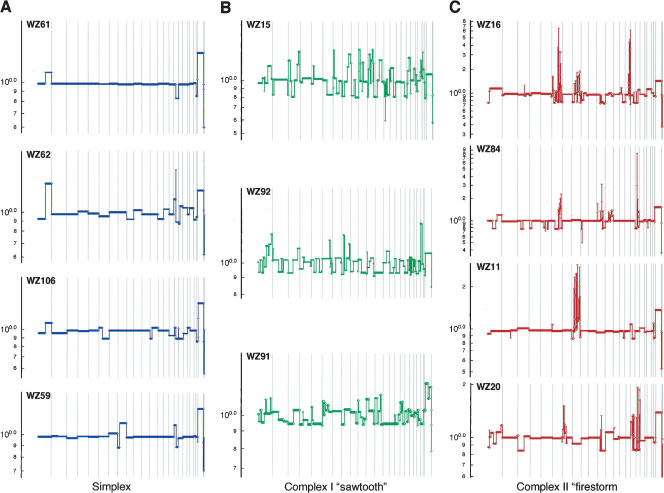
\includegraphics[width = 1\textwidth]{../figures/Chapter_2/Hicks_2006.jpg}
\caption[Distinct patterns of genomic rearrangements in breast cancer, taken from \cite{pmid17142309}.]{Distinct patterns of genomic rearrangements in breast cancer, taken from \cite{pmid17142309}. Segmentation profiles for individual tumours representing each category: (A) “Simplex” pattern (B) “Complex I”/“sawtooth” pattern (C) “Complex II”/“firestorm” pattern. The x-axis denotes chromosomes 1-22, X and Y, ordered from left to right, and the y-axis displays the geometric mean value of two experiments on a log scale.}
\label{fig:fig.hicks}
\end{figure}

Tumours displaying the “simplex” pattern have large segments of duplication and deletion that usually span entire chromosome arms or even chromosomes (Figure \ref{fig:fig.hicks}A). Frequent copy number changes observed within tumours displaying the “simplex” pattern include gain of chromosomes 1q, 8q and/or 16p and loss of chromosomes 16q, 8p and/or 22. These tumours are usually ER+ and of the Luminal subtype. Tumours displaying the “complex I” pattern, also termed the “sawtooth” pattern, have complex patterns of narrow, low-amplitude gains and losses. These gains and losses usually span short chromosome regions and are often alternating, resulting in regions with many copy number transitions (Figure \ref{fig:fig.hicks}B). These events commonly affect all chromosomes and lead to the majority of the genome undergoing copy number changes. Recurring copy number changes observed within tumours displaying the “complex I” pattern include regions of gain on chromosome 10p, and regions of loss on chromosomes 3p, 4p, 4q, 5q, 14q, 15q, and 17q. These tumours are usually triple-negative (ER-/PR-/HER-) and correspond to the Basal subtype. Tumours displaying the “complex II” pattern, also known as the “firestorm” pattern, resemble the “simplex” pattern except that the tumours contain at least one localised region of clustered narrow peaks of amplification, i.e. each amplification cluster is restricted to an individual chromosome or chromosome arm. These regions of amplification are referred to as amplicons and are usually separated by regions displaying normal copy number or deletions (Figure \ref{fig:fig.hicks}C). Recurrently amplified sites include FGFR1, MYC, CCND1, MDM2, ERBB2 (HER2), and ZNF217. These tumours are usually of the Luminal B and HER2 subtype. Tumours displaying the “flat” pattern have no clear amplifications or deletions except copy number polymorphisms \citep{pmid17142309, pmid28733194}. 

To relate these patterns to clinical outcome, \cite{pmid17142309} developed the Firestorm Index. Using this metric, it was observed that the “complex I” and “complex II” patterns were associated with more aggressive disease and worse survival outcomes. 

\cite{pmid27136393} provides a classification based on rearrangement signatures derived from 560 breast cancer whole genome sequences. Six rearrangement signatures (RS1-RS6) were created, based on whether the rearrangement was a deletion, tandem duplication, inversion, or translocation, the size of the rearrangement and also whether the rearrangements occurred in close proximity to each other. Interestingly, \cite{pmid28733194} noted that these signatures relate back to the classification described in \cite{pmid17142309}. RS1 and RS3 are characterised by tandem duplications similar to the “complex I” or “sawtooth” pattern, RS4 and RS6 by clustered rearrangements similar to the “complex II” or “firestorm” pattern, RS5 by deletions, and RS2 by translocations, similar to the “simplex” pattern. For most tumours, the genomic landscape of rearrangements is composed of combinations of these signatures \citep{pmid27136393, pmid28733194}.

\cite{pmid22522925} used gene expression data along with CNA data, of 1,992 breast cancer samples from the METABRIC cohort, to identify ten distinct subtypes of breast cancer. Initially, using Analysis of Variance (ANOVA) and the Kruskal-Wallis test, they identified genes where the presence of a CNA influenced the expression of that gene, i.e. where overexpression is associated with copy number gain or amplification and underexpression with copy number loss. This method, by definition, captures genomic drivers, oncogenes and tumour suppressor genes whose expression is associated with copy number changes. The 1,000 most significant cis-driven genes, in terms of Bonferroni corrected p-values, were inputted as explanatory variables in a joint latent variable framework for integrative clustering. The most parsimonious solution, with reference to copy number profiles, risk patterns, and prognosis, classified tumours into ten distinct groups (IntClust 1-10, Figure \ref{fig:fig.IC}). %Table \ref{tbl:IC}, produced by \cite{pmid23395906}, documents the features of the integrative clusters.

\begin{figure}[h]
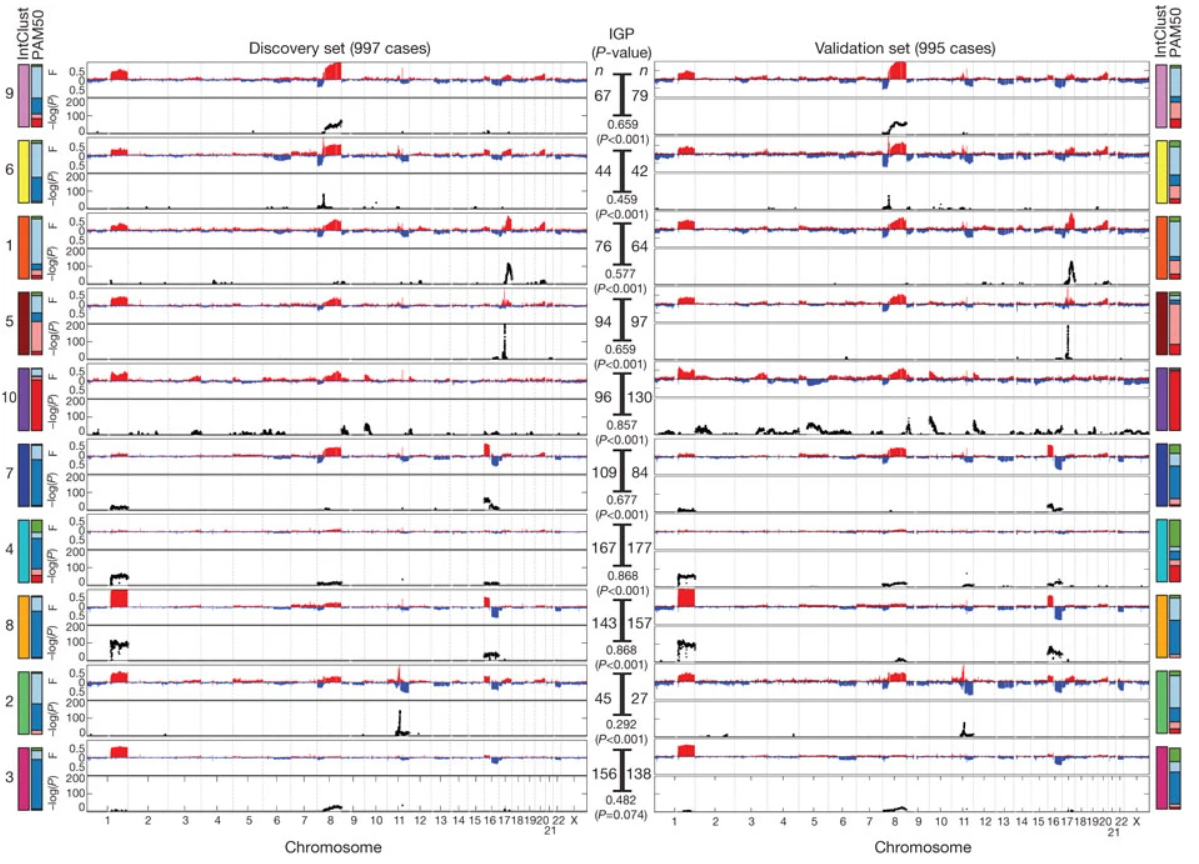
\includegraphics[width = 1\textwidth]{../figures/Chapter_2/IntClust_Profiles_Curtis.png}
\caption[Distinct copy number profiles of the Integrative Clusters, taken from \cite{pmid22522925}.]{Distinct copy number profiles of the Integrative Clusters, taken from \cite{pmid22522925}. Frequencies of CNAs are displayed on the upper y-axis of each section and the subtype-specific association (-log10 p-value) of aberrations is displayed on the bottom y-axis. Regions of copy number gain are indicated in red and regions of loss in blue. The distribution of PAM50 subtypes within each cluster is also shown.}
\label{fig:fig.IC}
\end{figure}

\subsection{Measures of Genomic Instability}
\label{MeasureGI} 
To explore the impact of GI in cancer, a number of genomic and transcriptomic signatures have been created to quantify levels of GI in tumours, and their prognostic and predictive power assessed. These metrics, summarised in Table \ref{tab:GI}, are described below.

% Please add the following required packages to your document preamble:
% \usepackage{graphicx}
\begin{table}[!htb]
\caption{Summary of existing measures of Genomic Instability.}
\resizebox{\textwidth}{!}{%
\begin{tabular}{|l|l|l|l|l|}
\hline
\textbf{GI Measure}                                                                                         & \textbf{Cancer Type(s)}                                                                                                                                                                   & \textbf{Input Data}  & \textbf{Platform(s) Used in Study}                                                                                                        & \textbf{Author}                                                                        \\ \hline
CIN25 and CIN75                                                                                             & \begin{tabular}[c]{@{}l@{}}Breast cancer, lung adenocarcinoma, \\ small-cell lung cancer, mesothelioma, \\ prostate cancer, B-cell lymphoma, \\ ovarian cancer, glioma, medulloblastoma\end{tabular} & Gene expression data & \begin{tabular}[c]{@{}l@{}}Affymetrix Human Genome \\ U133A microarray \\ Affymetrix Human Genome \\ U133+2 microarray \\ Rosetta 25k microarray\end{tabular} & \cite{pmid16921376} \\ \hline
Chromosomal Instability Score                                                                               & Breast cancer                                                                                                                                                                                        & Copy number data     & \begin{tabular}[c]{@{}l@{}}Affymetrix GeneChip Mapping \\ 100K microarray                                                                                           \end{tabular} & \cite{pmid20632083} \\ \hline
\begin{tabular}[c]{@{}l@{}} Centromere and Kinetochore \\ Gene Expression Score\end{tabular}
& \begin{tabular}[c]{@{}l@{}}Breast, lung, ovarian, liver, pancreatic, \\ colon, nasopharyngeal, gastric, cervical, \\ head and neck, prostate, brain.\end{tabular}                                     & Gene expression data & \begin{tabular}[c]{@{}l@{}}Affymetrix Human Genome \\ U133+2 microarray\end{tabular}                                                                                                         & \cite{pmid27577169}                                                                     \\ \hline
Chromosomal Instability Index                                                                               & Colorectal cancer                                                                                                                                                                                    & Copy number data     & \begin{tabular}[c]{@{}l@{}}Affymetrix Genome-wide Human \\ SNP array 6.0                                                                                            \end{tabular}  & \cite{pmid29343938} \\ \hline
\begin{tabular}[c]{@{}l@{}}Whole Arm Aberration Index and \\ Complex Arm‐Wise Aberration Index\end{tabular} & Breast cancer                                                                                                                                                                                        & Copy number data     & \begin{tabular}[c]{@{}l@{}}
Custom ROMA 85k microarray \\
Agilent Human Genome CGH \\ 244K microarray \\
Custom Human 30K 60-mer \\ oligo microarray
\end{tabular}                                                        & \cite{pmid20592421}                                                                   \\ \hline
Firestorm Index                                                                                             & Breast cancer                                                                                                                                                                                        & Copy number data & Custom ROMA 85k microarray & \cite{pmid17142309} \\ \hline
Copy Number Alteration Burden                                                                               & Prostate cancer, breast cancer                                                                                                                                                                       & Copy number data     & \begin{tabular}[c]{@{}l@{}}Agilent Human CGH Whole \\ Genome microarray \\ Affymetrix Genome-wide Human \\ SNP array 6.0 \end{tabular}                                                                                             & \begin{tabular}[c]{@{}l@{}}\cite{pmid25024180} \\ \cite{pmid30178746} \\ \cite{pmid30337938}\end{tabular} \\ \hline
\begin{tabular}[c]{@{}l@{}}Copy Aberration Regional Mapping \\ Analysis Scores \end{tabular}                                                            & Breast cancer                                                                                                                                                                                        & Copy number data     & \begin{tabular}[c]{@{}l@{}}Affymetrix Genome-wide Human \\ SNP array 6.0                                                                                            \end{tabular} & \cite{pmid32242091} \\ \hline
Genomic Instability Index                                                                                   & Breast cancer                                                                                                                                                                                        & Copy number data     & \begin{tabular}[c]{@{}l@{}}Custom Human 30K 60-mer \\ oligo microarray\end{tabular} & \cite{pmid17925008} \\ \hline
\begin{tabular}[c]{@{}l@{}}Genomic Identification of Significant \\ Targets in Cancer \end{tabular} & Glioma                                                                                                                                                                                               & Copy number data     & \begin{tabular}[c]{@{}l@{}}Affymetrix Human Mapping 50K \\ Xba240 SNP array\\ Affymetrix Human Mapping 50k \\ Hind240 SNP array\end{tabular} & \cite{pmid18077431}                                                                  \\ \hline
\end{tabular}%
}
\label{tab:GI}
\end{table}

\subsubsection{Expression Based Signature CIN25 and CIN70}
It has been well documented that correspondence exists between gene expression changes and CNAs in regions relevant to those genes \citep{pmid12297621, pmid17289997,  pmid22522925, pmid32024838}. \cite{pmid16921376} derived two expression-based signatures, reflecting CIN in tumours, termed CIN25 and CIN70, using 25 and 70 genes, respectively. These signatures were developed using integrated gene expression data from 18 studies, across nine cancer types, totalling 1,944 samples. These signatures are based on a functional aneuploidy measure (FA) calculated across cytobands, i.e. genomic regions corresponding to the approximate location of bands seen on Giemsa-stained chromosomes. For a given dataset, a cytoband specific \textit{t}-statistic compares normalised gene expression measurements mapped to a specific cytoband, group B, to the normalised gene expression measurements for the genes mapped to all other cytobands, group G: 

\begin{equation}
t = \frac{\mu_B - \mu_G}{\sqrt{(\frac{\sigma^2_B}{N_B}) + \frac{\sigma^2_G}{N_G})}}
\end{equation}

where $\mu_B$, $\mu_G$ are the observed means, $\sigma^2_B$,  $\sigma^2_G$, are the observed variances, and $N_B$, $N_G$, the number of genes, for groups B and G.

The total FA (tFA) for each sample, within each of the 18 datasets, was defined as the sum of all FA magnitudes (the absolute \textit{t} statistics), across each cytoband with more than 10 genes recorded, in that sample. For all genes within each dataset, the correlation coefficient across all samples between each gene's expression vector (the vector containing that genes expression for all samples in that dataset) and the tFA vector (the vector containing the tFA for each sample in that dataset) was computed. Genes in each dataset were then ranked based on the value of the correlation coefficient. Following normalisation of ranks within each dataset, the total of the ranks of a gene within three selected datasets was used as the final integrated ranking for the gene. The top 25 and 70 genes from this ranking formed the CIN25 and CIN70 signature, respectively.

tFA was found to be significantly correlated with aneuploidy assessed using CNA profiles and structural chromosomal aberrations from spectral karyotyping on NCI-60 cell lines. Furthermore, the CIN25 and CIN70 genes showed significant deviation in their expression relative to the remainder of the transcriptome and were enriched for regulators of mitotic spindle assembly, the mitotic checkpoint, and the DNA damage checkpoint.

To explore the prognostic power of CIN25 and CIN70, patients were split into two groups, patients with total expression, i.e. sum of the log-ratio measures, above the mean signature expression, and patients below the mean signature expression, in all samples from that dataset. This indicated that the CIN25 signature was a significant predictor of clinical outcome in 12 out of 18 cancer datasets and the CIN70 signature was a significant predictor of clinical outcome in 13 out of 18 datasets. Comparing the CIN25 and CIN70 signatures between primary and metastatic tumours also indicated metastatic samples display higher levels of the CIN signatures compared to primary tumours.

\subsubsection{Chromosomal Instability Score}
\cite{pmid20632083} used SNP copy number data from 313 primary lymph-node negative breast cancers to study the prognostic relevance of CIN within breast cancer subtypes. In this study, by measuring the loss, gain, or diploid status of SNPs within 100-kilobase (kb) genomic windows, a measure for CIN was defined as the total number of chromosomal segments showing a gain or loss. Hierarchical clustering of patients using this CIN metric identified four main groups showing varying degrees of chromosomal abnormalities. In addition, it was found that high CIN score was significantly associated with worse prognosis in ER+, Luminal B, and HER2 subtypes, but not in ER- patients. 

\subsubsection{Centromere and Kinetochore Gene Expression Score}
Centromeres and kinetochores play essential roles in cell division and their protein level is usually tightly regulated \citep{pmid19002142}. Their dysfunction can result in a number of misregulation effects, including missegregation and mislocalisation to non-centromeric chromatin, generating neo-centromeres, dicentric behaviour and chromosome bridges, that drive aneuploidy and CIN (gains and losses) \citep{pmid19002142, pmid27577169}. To capture this misregulation, \cite{pmid27577169} developed the centromere and kinetochore gene expression score (CES) that quantifies the misexpression of 14 centromere and kinetochore genes in cancers. To arrive at this scoring mechanism, expression profiles of 31 candidate centromere and kinetochore genes were analysed, 15 of these genes were observed to be significantly misregulated and of these, 14 were found to be associated with poor patient survival and correlated with cancer progression, in an analysis of 18 different cancer datasets from The Cancer Genome Atlas (TCGA). CES is calculated as the sum of the log$_2$ mRNA expression level of the 14 centromere and kinetochore genes. It was shown that high CES significantly correlated with increased CIN and accurately predicts patient outcome in terms of OS, distant metastasis-free survival and relapse-free survival. This study also reported that high CES cell lines were sensitive to genotoxic drugs, such as campthothecin, topotecan and irinotecan.

\subsubsection{Chromosomal Instability Index}
The CIN index is a measurement that quantitatively characterises genome-wide CNAs. The CINdex algorithm uses segmented copy number data to calculate global measures of GI across chromosomes and at a higher resolution across cytobands. The first step in calculating CIN index involves calling segments as either gain or loss. A segment with mean signal intensity greater than an assigned threshold, $t_{gain}$, is called as a gain, whereas a segment with mean signal intensity smaller than an assigned threshold, $t_{loss}$, is called as a loss. In \cite{pmid29343938} the biologically experimental values of $t_{gain}$ and $t_{loss}$ are 2.5 and 1.5, respectively. Subsequently, the amplitude of change is scaled to make maximal losses and maximal gains comparable in magnitude. To do this, the amplitude of each loss segment, $a$, is converted to the new value, $a'$, based on the relationship given by: 

\begin{equation}
(t_{loss} - a)/a = (a'-t_{gain})/(A - t_{gain})
\end{equation}

where $A$ is maximum gain amplitude across all samples and segments and $t_{loss}$ and $t_{gain}$ are the assigned thresholds for calling losses and gains, respectively. 

The chromosome-specific instability index for each sample is calculated using:

\begin{equation}
CIN_i = (\sum_ka_k + \sum_ja'_j)/N
\end{equation}

where \textit{N} is the number of SNP probes on chromosome $i$, $a$ is the amplitude of gain segments and $a’$ is the amplitude of loss segments. 

Applying the same calculation at the cytoband level provides the cytoband-specific instability index. The CINdex Bioconductor package \citep{CINdex} implements this algorithm and generates a chromosome and cytoband CIN value for each sample. The package also enables comparison of CIN index values between groups of patients to identify differentially altered chromosomes or cytobands. Genes within these differentially altered regions can then be identified and pathway enrichment performed. 

\subsubsection{Whole Arm Aberration Index and Complex Arm‐Wise Aberration Index}
\cite{pmid20592421} developed two algorithms to characterise levels of genomic distortion using array comparative genomic hybridisation (aCGH) data. These algorithms are termed the Whole Arm Aberration Index (WAAI) and the Complex Arm Aberration Index (CAAI), where WAAI aims to capture whole-arm deviations from normal copy number, i.e. whole-arm gains/losses, and CAAI aims to capture the degree of local distortion i.e complex rearrangements. 

WAAI is calculated across each chromosome arm for each sample. The first step in generating the WAAI values is to use the Piecewise Constant Fitting (PCF) algorithm to fit a piecewise constant regression function to the log-transformed aCGH data for each sample. As a result, a fitted value, termed “PCF-value”, is obtained for each probe. The centred PCF-values were then divided by the residual standard deviation to produce normalised PCF (NPCF)-values and a new variable $s$ was obtained by averaging the NPCF-values over all probes. If $s > 0$, WAAI was the 5\% quantile of NPCF and if $s \leq 0$, WAAI was the 95\% quantile of NPCF. Chromosome arms with WAAI $\ge 0.8$ were called as whole-arm gains, and chromosome arms with WAAI $\leq -0.8$ were called as whole arm losses. 

CAAI is also calculated across each chromosome arm for each sample. In the original paper a threshold of 0.5 was applied to create a two-category CAAI variable, whereas it is possible to use the CAAI as a continuous variable \citep{pmid32242091}. The first step in generating the CAAI variable is to use the PCF algorithm to fit a piecewise constant regression function to the log-transformed aCGH data for each sample. Then for each breakpoint (chromosomal position affected by rearrangements) identified by PCF, three scores, P, Q and W, were calculated. To produce the CAAI variable from the original paper, P, Q and W are defined as follows: 

\begin{equation}
P = tanh \left( \frac{\alpha}{L1 + L2} \right)
\end{equation}
\begin{equation}
Q = tanh(|H2 - H1|)
\end{equation}
\begin{equation}
W = 0.5 \left[1 + \frac{tanh(10(P-0.5))}{tanh(5)} \right]
\end{equation}

where $\alpha$ is a constant. For any given breakpoint, $L1$ and $L2$ denote the number of nucleotides in each segment and $H1$ and $H2$ denote their scaled PCF-values.  

\cite{pmid32242091}, proposed a refined version of the CAAI variable, where P, Q and W are defined as: 

\begin{equation}
P = tanh \left(\frac{\alpha}{L1 + L2} \right)
\end{equation}
\begin{equation}
Q = tanh(\beta \cdot |H1 - H2|)
\end{equation}
\begin{equation}
W = 0.5 \left[1 + \frac{tanh(10P - 5)}{tanh(5)} \right]
\end{equation}

where $\alpha$ and $\beta$ are constants $2 \cdot 10^6$ and $\frac{1}{1.2}$, respectively. For any given breakpoint, $L1$ and $L2$ denote the size of the segments joined and $H1$ and $H2$ denote their height, i.e. total copy number. 

These three scores P, Q and W, reflect the proximity to neighbouring breakpoints, the magnitude of change and a weight of importance. Subsequently, CAAI is defined as the maximal value of $\sum W \cdot min(P, Q)$ across all breakpoints within a region of predefined size, i.e. 20 megabases (Mb).

Applying CAAI and WAAI to data from 595 breast cancer patients from four clinical cohorts (MicMa cohort, WZ cohort, Chin-UCAM cohort and Ull cohort), patients were split into eight subgroups each with distinct patterns of genomic alterations. CAAI was observed to be highly prognostic for DSS and OS in breast cancer. In addition, CAAI also correlates with expression-based prognostic signatures including MammaPrint and OncotypeDX. Subsequently, \cite{pmid25169931} validated CAAI as an independent prognostic indicator in breast cancer and also showed that CAAI could act as a prognostic indicator in high-grade serous ovarian cancer.

\subsubsection{Firestorm Index}
\label{MeasureGIFI}
\cite{pmid17142309} noted that the “complex I”/“sawtooth” and “complex II”/“firestorm” patterns often correlated with aggressive disease and worse survival in diploid tumours. To confirm this, the authors created a metric which separates the highly rearranged “complex I”/“sawtooth” and “complex II”/“firestorm” from the “flat” and “simplex” patterns. To distinguish the “complex II”/“firestorm” pattern from the “simplex” pattern this metric considered both the tightly packed spacing of the firestorm events and the total number of events. This metric, termed the Firestorm index (F), is obtained by summation across the reciprocals of the mean of lengths of all adjacent segment pairs: 

\begin{equation}
F = \sum_i{\frac{2}{l_i^L + l_i^R}}
\end{equation}

where $i$ corresponds to the set of all discontinuities or breaks with a magnitude above the threshold of 0.1, $l_i^L$ and $l_i^R$ correspond to the number of probes in the nearest discontinuity to the left or right, respectively, or to a chromosome boundary, whichever is closer.

This metric can distinguish the “complex II”/“firestorm” pattern from the “simplex” pattern and assigns high F values to the complex patterns. The “complex I”/“sawtooth” pattern will have a high F value as a result of the high number of events across a large number of chromosomes, while the “complex II”/“firestorm” pattern will have a high F value due to the sparse events occurring in close proximity. \cite{pmid17142309} also reported a strong association between F and survival outcomes.

\subsubsection{Copy Number Alteration Burden}
\label{CNABurden}
CNA Burden is defined as a measure of the percentage of the genome affected by CNAs, calculated as the summation of the lengths of all CNA (gain and loss) segments as a percentage of the total length of the autosomal genome. 

A number of studies have reported an association between CNA burden and recurrence, metastasis, OS and DSS \citep{pmid25024180, pmid30178746, pmid30337938}. \cite{pmid25024180} showed that CNA burden is prognostic for prostate cancer recurrence and metastasis, \cite{pmid30178746} observed that CNA burden is associated with both OS and DSS in a range of cancers including breast, endometrial, renal, thyroid, and colorectal cancer and \cite{pmid30337938} showed that there is a significant association between CNA burden and OS and DSS in breast cancer cohorts.

\subsubsection{Copy Aberration Regional Mapping Analysis Scores}
\label{CARMA}
\cite{pmid32242091} developed the Copy Aberration Regional Mapping Analysis (CARMA) algorithm which identifies multiple local copy number features, or “motifs”, across a pre-defined region and combines these to create regional metrics. CARMA takes allele-specific copy number profiles as inputs and produces six metrics that aim to capture the degree of amplification (AMP), deletion (DEL), complexity, i.e. chromothripsis and chromoplexy (STP and CRV), loss of heterozygosity (LOH) and allelic imbalance or asymmetry (ASM). Together, these metrics consider copy number magnitude, the spatial distribution of copy number breakpoints, allelic imbalance and regional fluctuations in copy number.  

These scores are defined using continuous functions on genomic loci, i.e. positions on a chromosome, $t_1, …, t_i$, over a region R. Here, $f(t)$ is the median centred total copy number in locus $t$ and is calculated by $f(t) = f_A(t) + f_B(t) - m$, where $f_A(t)$ and $f_B(t)$ are piecewise constant functions representing the allele-specific copy number profiles of the major allele and minor allele, respectively, and $m$ is chosen as the median observed copy number.   

The degree of amplification AMP is defined as:

\begin{equation}
AMP = \int_{R}{\{f(t)_+\}^2} 
\end{equation}

where $f(t)_+$ corresponds to the regions where the median centred total copy number is greater than 0. Alternatively, one can think of this metric as $AMP = \sum L_+ \times H_+^2$, where $L_+$ is a vector containing the scaled lengths of segments where an amplification is present, relative to the median copy number, and $H_+$ is a vector containing the corresponding copy number magnitudes. AMP will take value 0 where the total copy number is equal to the median copy number and greater than 0 when there are some gains and no losses relative to the median. 

Similarly, the degree of deletion is defined as: 

\begin{equation}
DEL = \int_{R}{\{f(t)_-\}^2}
\end{equation}

where $f(t)_-$ corresponds to the regions where the median centred total copy number is less than 0. DEL will take value 0 where the total copy number is equal to the median and greater than 0, where there are some losses and no gains relative to the median.   

The complexity scores are defined as: 

\begin{equation}
STP = \int_{R}{\{Df(t)\}^2} dt
\end{equation}
\begin{equation}
CRV = \int_{R}{\{D^2f(t)\}^2} dt
\end{equation} 

where $Df(t)$ is the first derivative and $D^2f(t)$ is the second derivative, reflecting the change in total copy number and the oscillation in total copy number, respectively. STP will take value 0 where there is constant total copy number and greater than 0 where there is gradually increasing or decreasing copy number, or where there are fluctuations between smaller and larger copy numbers. CRV will take value 0 where the copy number is constant, be close to 0 where there is gradually increasing or decreasing copy number and greater than 0 where there are fluctuations between smaller and larger copy numbers. 

Loss of heterozygosity is defined as: 

\begin{equation}
LOH =  \int_{R}{\{1_0(f_B(t))\}} dt
\end{equation}

where $f_B(t)$ is the piecewise constant function representing the copy number profile of the minor allele, $1_0$ is an indicator variable informing whether or not the minor allele is lost. If the copy number of the minor allele is 0 at locus $t$ then $1_0 = 1$, otherwise $1_0 =0$. Alternatively, one can think of this metric as $LOH = \sum L[minor = 0]$, where $L$ is a vector containing the scaled lengths of segments where the minor allele has been lost, i.e. copy number is 0. LOH takes a value greater than 0 where the minor allele has been lost, with the magnitude of the metric reflecting the proportion of the region with LOH. 

Allelic imbalance or asymmetry is defined as:  

\begin{equation}
ASM = \int_{R}{\{(f_A(t) - f_B(t))^2\}} dt
\end{equation}

where $f_A(t)$ and $f_B(t)$ are the piecewise constant functions representing the copy number profile of the major allele and the minor allele, respectively, so that ASM $> 0$ in regions of allelic imbalance. 

The authors applied CARMA to four breast cancer cohorts, METABRIC (n = 1,943), Oslo2 (n = 276), OsloVal (n = 165), and ICGC (n = 553). To standardise the scores, all six scores were log$_2$-transformed and normalised by dividing by the 99th percentile in the METABRIC discovery set. The authors showed that the CARMA metrics correlated with the CAAI and CINdex metrics and provided significantly more detail about the copy number profile, enabling identification of alterations that may not be captured by the other methods. For example, in a region where there is loss of one allele and gain of the other, the CINdex would indicate that no alteration has occurred, whereas the LOH and ASM metrics would capture this event. The authors also considered the distribution of CARMA scores within breast cancer subtype classifications (PAM50 and IntClust) and noted that the CARMA scores captured differences in the genomic landscapes of the distinct subtypes. 

Examining whether the CARMA metrics were significantly associated with survival outcome, univariate Cox proportional hazards regression models were fitted for each metric, and these models indicated that all CARMA metrics were associated with DSS. To assess if the presence or absence of the copy number motifs was significantly associated with survival outcome, the information provided by all six CARMA metrics was combined into two prognostic indices, the CARMA Prognostic Index (CPI) and the weighted CPI ($\text{CPI}_\text{weighted}$). Briefly, using a discovery set and test set from the observed cohort, the CPI index was produced by fitting multivariate Cox regression models for DSS outcome and progression-free survival outcome, using the unweighted mean of the six CARMA metrics as predictors. The fitted model was then applied to the test set, producing a single unweighted prognostic value for each patient in the test set. 

Patients were stratified into low, intermediate, and high-risk groups, of equal cohort size, based on their CPI value. These tertile groups are defined as having CPI score, 1, 2, and 3, respectively. The $\text{CPI}_\text{weighted}$ score was produced using the 252 arm-wise CARMA scores directly as predictors and fitting a Cox regression model with LASSO penalty to the discovery set. Coefficients derived from the model were then used as weights to calculate the $\text{CPI}_\text{weighted}$. Both CPI and $\text{CPI}_\text{weighted}$ were shown to be significantly associated with DSS and progression-free survival before and after adjusting for other relevant clinical variables. Patients in the high-risk CPI group displayed significantly worse DSS and progression-free survival.

\subsubsection{Genomic Instability Index}
The Genomic Instability Index (GII) is defined as the fraction of the genome with CNAs. \cite{pmid17925008} proposed two GII metrics, calculated based on the fraction of the genome that was altered using common regions of alteration (CRA), regions that were altered in at least 5\% of tumours, and on the fraction of altered probes. As expected, a very strong correlation was observed between the two GII metrics (Spearman rank correlation 0.96). Using hierarchical clustering, on the CRA from 171 primary breast tumours, the authors identified a novel subtype of high-grade ER- breast cancer, characterised by a low GII. With this index the authors documented regions across the breast cancer genome that frequently contain CNAs and have corresponding dysregulated expression. Furthermore, they identified regions of the genome that were frequently amplified and correlated with poor prognosis, with some of these regions not previously identified. 

\subsubsection{Genomic Identification of Significant Targets in Cancer} 
\cite{pmid18077431} introduced the Genomic Identification of Significant Targets in Cancer (GISTIC) algorithm which differs from the previously mentioned GI measures/algorithms in that it identifies regions within the genome that are significantly altered across multiple samples. GISTIC produces multiple outputs, including a categorical value (0, 1 or 2) of aberration for each region and each sample. The GISTIC algorithm first assigns a score (G score) to each aberration, which reflects the aberration amplitude and the frequency with which the aberration occurs across samples, the significance of each aberration is assessed using permutation tests based on the overall pattern of aberrations observed across the genome. Regions with false discovery rates below a given threshold are declared to be significant aberration regions. For each significant aberration region, GISTIC defines a “peak region”, containing the highest frequency and amplitude of aberration, and determines whether the signal is due to broad events, focal events, or both.    
GISTIC has been applied to multiple cancer types and has identified a number of new targets of deletions and amplifications such as EHMT1 in medulloblastoma and CDK8 in colorectal carcinoma \citep{pmid21527027}. 
 
In subsequent years, the GISTIC algorithm underwent a number of methodological improvements resulting in GISTIC2.0 \citep{pmid21527027}. These improvements address challenges relating to modelling of complex cancer genomes that contain a mixture of CNA types occurring at distinct background rates and the ability of copy-number algorithms to provide a priori statistical confidence. 

\subsubsection{Summary}
As discussed, a large number of measures to quantify GI in tumours exist in the literature. All these measures, except for CES, use regions of altered copy number as a measure of CIN and should, in theory, be comparable when dealing with simple copy number deviations. For more complex copy number patterns, such as copy-neutral loss of heterozygosity, certain measures perform better, i.e. CARMA LOH and ASM metrics capture the event, while CINdex does not. These measures derived and evaluated using array-based data, aCGH and SNP arrays, or whole genome sequencing data, are limited in their accessibility and use as access to raw or segmented array/whole genome sequencing data is required. In addition, they can often be hard to interpret. As a result, we aim to create easily interpretable GI measures that can be calculated using publicly available summary CNA data. These CNA metrics aim to capture the main aspects of CNAs, including magnitude, type and genomic location.

\subsection{Proposed Copy Number Alteration Metrics}
\label{PCNA} 
The following CNA metrics, termed CNA Score and Burden metrics, aim to quantify levels of GI from summary CNA data and consider the magnitude of the CNA and if the CNA is an amplification or deletion. The CNA calls range from -2 to +2 indicating homozygous deletion (-2), hemizygous deletion (-1), diploidy (0), single copy gain (+1) and high-level amplification (+2).

\subsubsection{Copy Number Alteration Score Metrics}
Absolute CNA Score (Equation \ref{eq:CNA1}) for a sample or patient is the summation across all genes, $g \in 1:G$, of the absolute magnitudes of all calls, irrespective of type, while CNA Amp Score and CNA Del Score, capture the total magnitudes of amplifications only (Equation \ref{eq:CNA2}) and the total magnitudes of deletions only (Equation \ref{eq:CNA3}). The Difference Score (Equation \ref{eq:CNA4}) measures the difference between the magnitudes of CNA Amp Score and CNA Del Score. The last two proposed CNA Score metrics measure the percentage of a patient's total CNA Score that is classified as amplifications (Equation \ref{eq:CNA5}) and the percentage classified as deletions (Equation \ref{eq:CNA6}). Notably, the percentage CNA metrics are correlated with each other, i.e. if for a patient the percentage amplified is $80\%$, then the percentage deleted will be $20\%$.

\begin{equation}
\text{Absolute CNA Score}\: = \frac{}{}\sum_{g = 1}^{G}\left | \:CNA\:\:call_g\: \right |
\label{eq:CNA1}
\end{equation}

\begin{equation}
\text{CNA Amp Score}\: = \frac{}{}\sum_{g = 1}^{G}\left | \:CNA\:\:Amp\:\:call_g\: \right |
\label{eq:CNA2}
\end{equation}

\begin{equation}
\text{CNA Del Score}\: = \frac{}{}\sum_{g = 1}^{G}\left | \:CNA\:\:Del\:\:call_g\: \right |
\label{eq:CNA3}
\end{equation}

\begin{equation}
\text{Difference Score}\: =  \:CNA\:\:Amp\:\:Score\: - \:CNA\:\:Del\:\:Score\:
\label{eq:CNA4}
\end{equation}

\begin{equation}
\text{Percentage Amp Score}\: = \frac{\:CNA\:\:Amp\:\:Score\:}{\:Absolute\:\:CNA\:\:Score\:}\times100
\label{eq:CNA5}
\end{equation}

\begin{equation}
\text{Percentage Del Score}\: = \frac{\:CNA\:\:Del\:\:Score\:}{\:Absolute\:\:CNA\:\:Score\:}\times100
\label{eq:CNA6}
\end{equation}

\subsubsection{Copy Number Alteration Burden Metrics}
Further, we propose calculation of several CNA Burden metrics, measured for each patient. It is important to note that our CNA Burden metrics (Equations \ref{eq:CNAB1}-\ref{eq:CNAB6}) differ from the CNA Burden metric \citep{pmid25024180} mentioned in Section \ref{CNABurden}. While both metrics aim to measure the percentage of the genome affected by CNAs, our CNA Burden metric uses publicly available gene level summary CNA data to calculate the percentage of genes containing an alteration, whereas the pre-existing metric uses the CNA segment lengths obtained from segmented CNA data to calculate the percentage of the genome affected by CNAs. Therefore, the focus here is on the presence of a CNA for each gene, while the CNA Burden metric utilised by \cite{pmid25024180} focuses on the lengths of these altered segments in relation to the total length of the autosomal genome. The proposed CNA Burden metric here also differs from the proposed CNA Score metric in several ways, including considering the presence or absence of a CNA rather than the magnitudes, and the scale and range of measurement, i.e. summation versus percentage.   

Absolute CNA Burden (Equation \ref{eq:CNAB1}) reflects the percentage of genes recorded containing an alteration. Similarly, the CNA Amp Burden metric (Equation \ref{eq:CNAB2}) and CNA Del Burden metric (Equation \ref{eq:CNAB3}) capture the percentage of genes containing an amplification and deletion, respectively. The Difference Score (Equation \ref{eq:CNAB4}) measures the difference between the CNA Amp Burden and CNA Del Burden. The last two proposed CNA Burden metrics measure the percentage of a patient's total CNA Burden that is classified as amplifications (Equation \ref{eq:CNAB5}) and the percentage classified as deletions (Equation \ref{eq:CNAB6}).

\begin{equation}
\text{CNA Burden}\: = \frac{\sum_{g = 1}^{G}  Alt_g}{G}\times100
\label{eq:CNAB1}
\end{equation}

\begin{equation}
\text{CNA Amp Burden}\: = \frac{\sum_{g = 1}^{G} {AltAmp}_g}{G}\times100
\label{eq:CNAB2}
\end{equation}

\begin{equation}
\text{CNA Del Burden}\: = \frac{\sum_{g = 1}^{G} {AltDel}_g}{G}\times100
\label{eq:CNAB3}
\end{equation}

\begin{equation}
\text{Difference Burden}\: = \:CNA\:\:Amp\:\:Burden\: - \:CNA\:\:Del\:\:Burden\:
\label{eq:CNAB4}
\end{equation}

\begin{equation}
\text{Percentage Amp Burden}\: = \frac{CNA\:\:Amp\:\:Burden\:}{CNA\:\:Burden\:}\times100
\label{eq:CNAB5}
\end{equation}

\begin{equation}
\text{Percentage Del Burden}\: = \frac{CNA\:\:Del\:\:Burden\:}{CNA\:\:Burden\:}\times100
\label{eq:CNAB6}
\end{equation}

$Alt$ corresponds to the alteration status (0 or 1) for each gene $g$, $AltAmp$ corresponds to the amplification status (0 or 1) for each gene $g$, and $AltDel$ corresponds to the deletion status (0 or 1) for each gene $g$.

\subsection{Application of CNA Metrics to the METABRIC Cohort}
These CNA Score and Burden metrics are calculated for all breast cancer patients in the METABRIC cohort for which CNA data were available (n = 2,173). The metrics are calculated globally, i.e. over all 22,544 genes recorded, and, more locally, for each of the 42 chromosome arms, to account for the genomic location of the CNA. It should be noted that chromosomes differ in length and number of genes, with chromosome 1 being the longest autosomal chromosome and chromosome 22 being the shortest autosomal chromosome, meaning the CNA Score metrics are not comparable across chromosomes. 

\subsubsection{Observed Distributions for Global CNA Metrics}
The observed distributions of the global CNA Score and Burden metrics are explored and summarised in Tables \ref{tab:Score_All}-\ref{tab:Burden_CCA}, along with density plots and histograms (Figure \ref{fig:Score_Comp_Dense} and Figure \ref{fig:Burden_Comp_Dense}).   

A large proportion of patients display some level of GI, 99.95\% with Absolute CNA Score $>0$ and 95\% with Absolute CNA Score $>100$. The distribution of the CNA Del Score is broader than the distribution of the CNA Amp Score, standard deviation 3,150.91 compared to 2,252.74, with a higher maximum score value of 14,530, indicating that a patient's genome may undergo higher levels of deletion than amplification (Table \ref{tab:Score_All}). This feature is also indicated in the Difference Score distribution, where there is a higher density of patients displaying negative difference values, mean -378.86 and median -8, indicating higher levels of deletion than amplification. Similar trends are observed in the CNA Burden distributions, where the standard deviations of the CNA Amp and Del distributions are 8.54 and 13.89, respectively, with a higher maximum burden value of 64.17 for the CNA Del distribution (Table \ref{tab:Burden_All}). 

To determine the impact of missingness on the CNA metrics, an assessment using only complete-case (CC) data, i.e. including only patients that have CNA information for all 22,544 genes recorded, versus using all available data to produce the CNA metrics is carried out. When using all available data, CNA metrics for all $2,173$ patients are produced, while CNA metrics calculated using only CC data discard patients displaying an NA value in any of the genes, leaving $2,091$ patients for which CNA metrics are calculated. It should be noted for the CNA Burden calculation, $G$ refers to the number of genes recorded for each patient and ranges from $22,466$ to $22,544$, when using all available data, and is $22,544$ when using the CC data. The main advantage of using CC data is simplicity, as statistical analysis is more straightforward with CC data. Disadvantages of using CC data stem from the potential loss of information in discarding incomplete cases. 

The effect of any missingness is assessed by comparing the features of the observed distributions for CC data and all data, using comparative density plots and estimating the overlapping area of the two kernel densities, using the R \texttt{overlap()} function \citep{Overlap}. This function is used to estimate the proportion of overlapping area between two densities, i.e. where the integral of the minimum between two densities is divided by the integral of the maximum of the two densities. This proportion is then multiplied by 100 to calculate the percentage overlap. 

Figure \ref{fig:Score_Comp_Dense} and Table \ref{table:CNAScoreT1} indicate that the two density plots for each global CNA Score metric are similar and have a high percentage overlap. The lowest percentage overlap, observed within Absolute CNA Score and CNA Del Score were 96.55\% and 97.15\%, respectively. High concordance is also observed in the comparison between the CNA Burden metrics (Figure \ref{fig:Burden_Comp_Dense} and Table \ref{table:CNABurdenT1}). The CNA Burden metrics displaying the lowest percentage overlap are CNA Burden and CNA Del Burden with 96.76\% and 97.18\%, respectively.

\vfill
\begin{figure}[!h]
\center
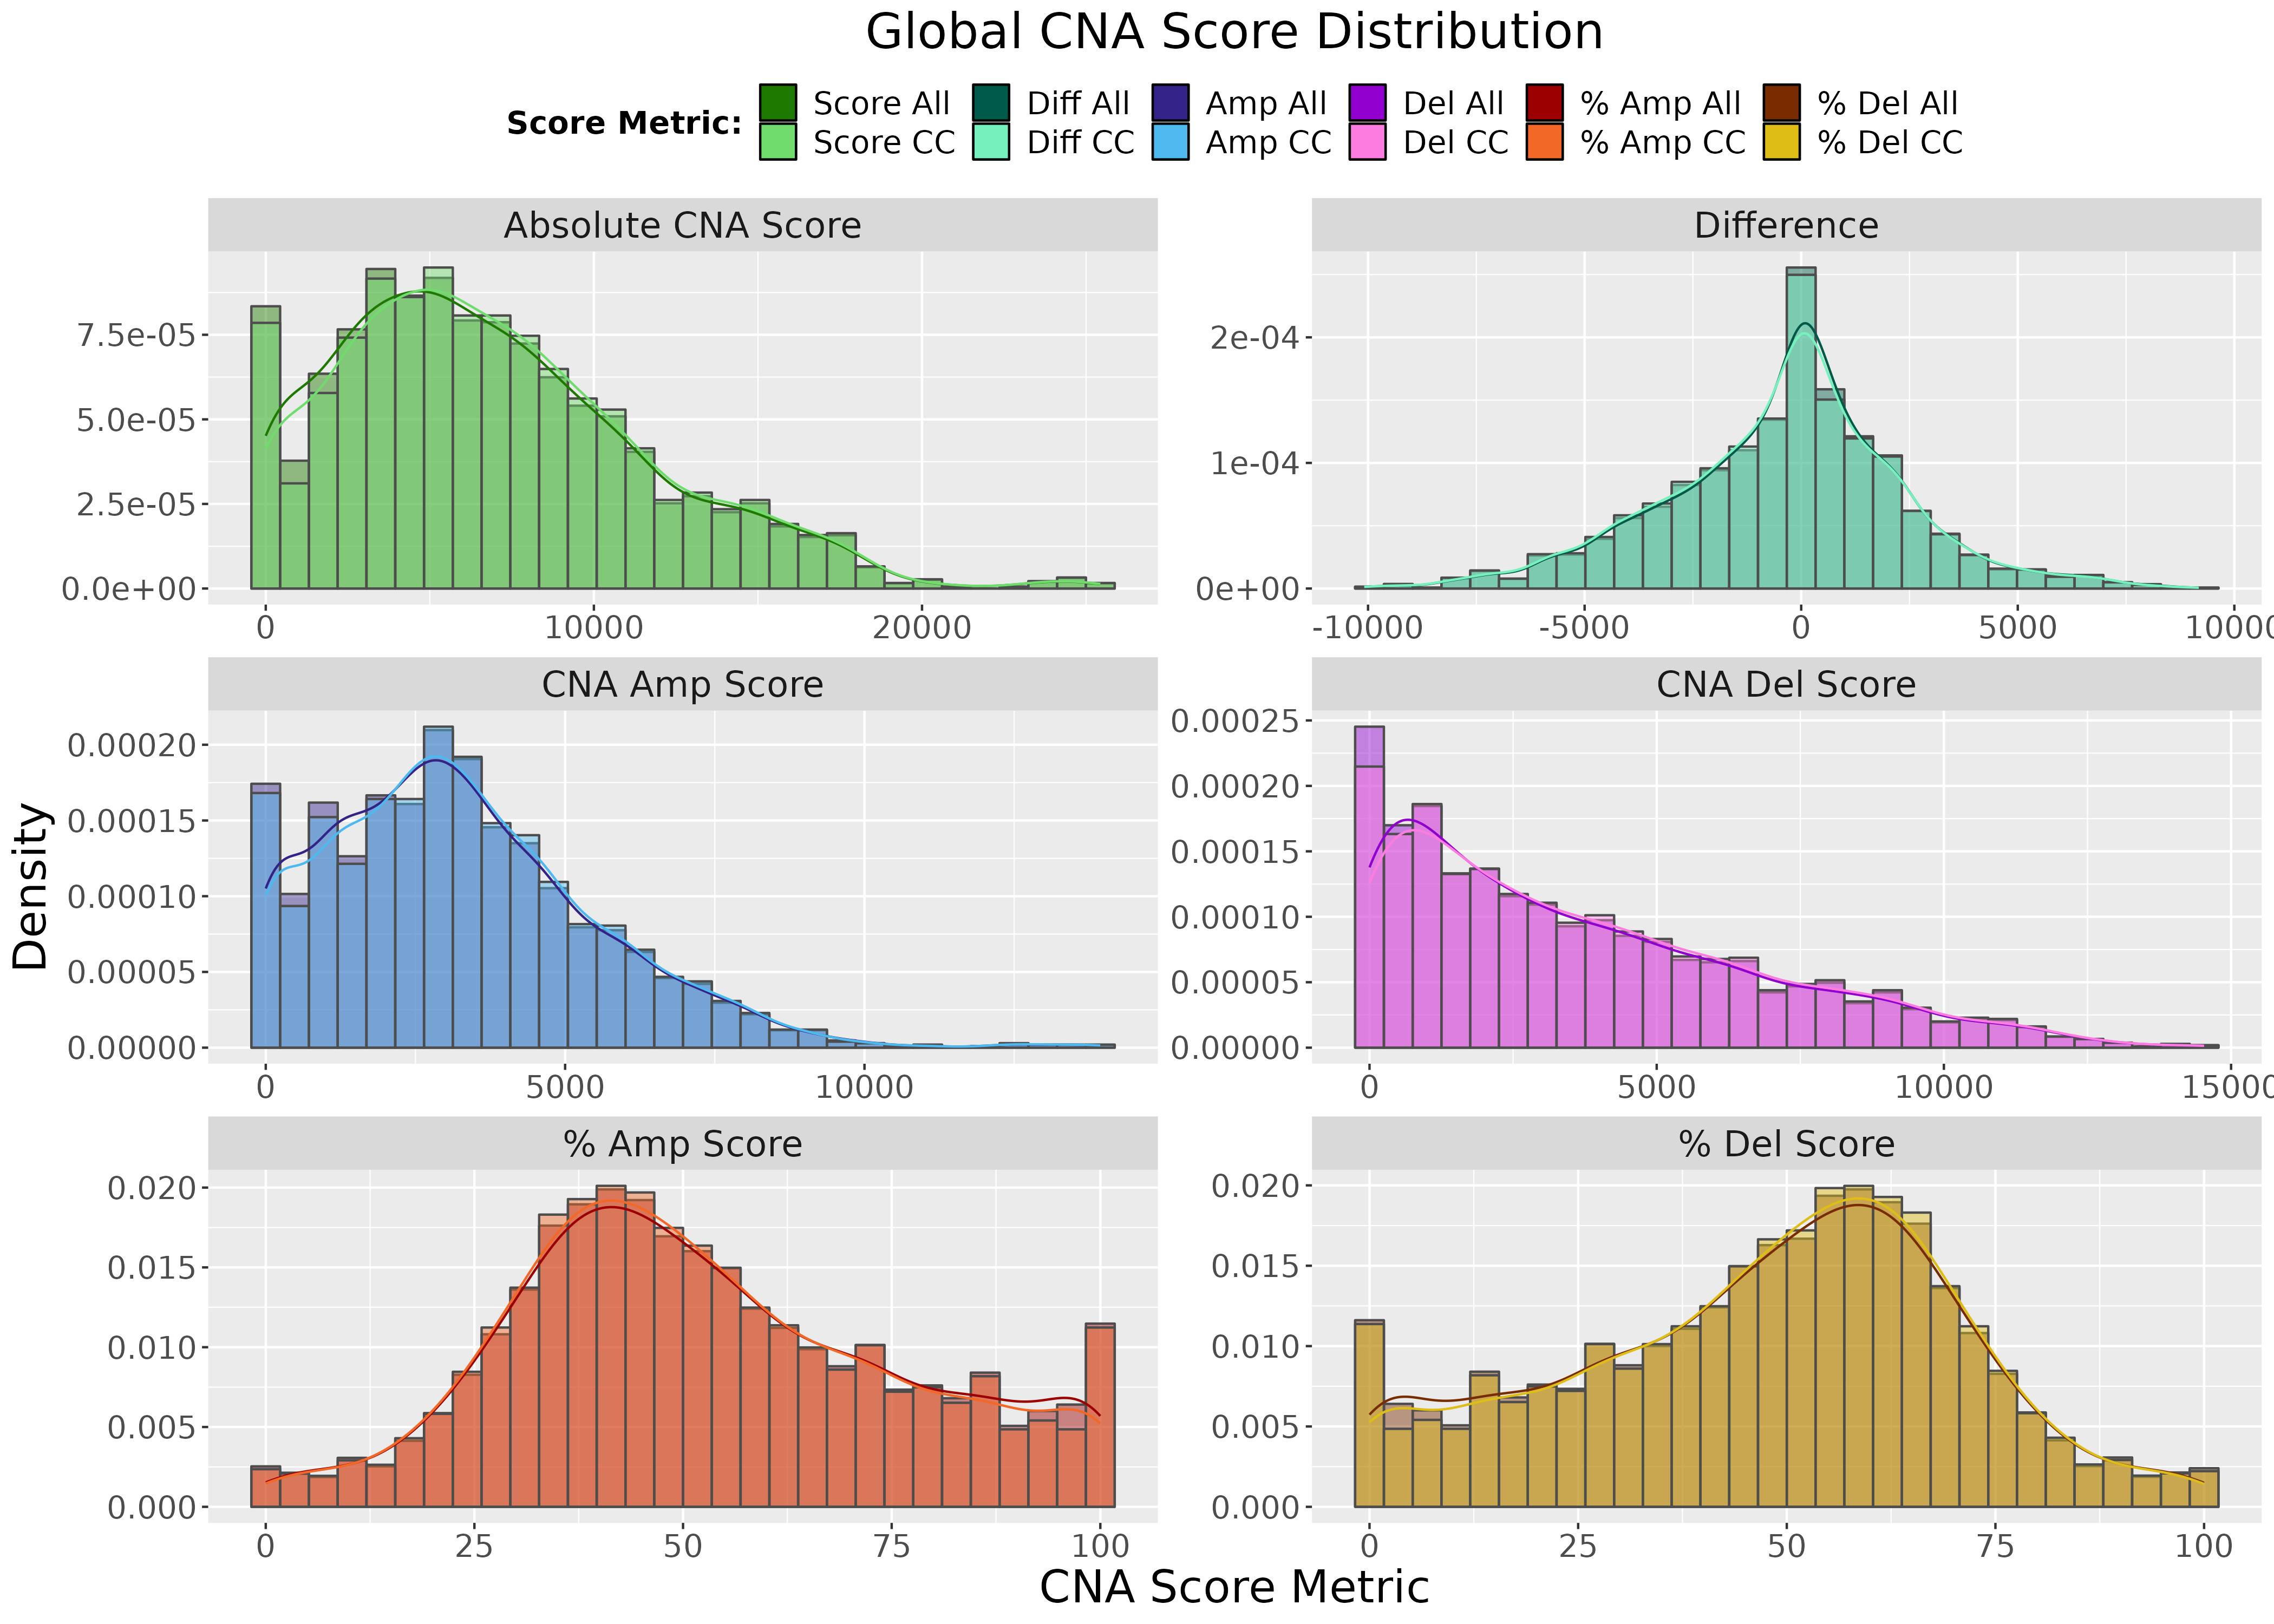
\includegraphics[width = 1\textwidth]{../figures/Chapter_2/Global_CNA_Score_Comparative_Density.png}
\caption[Density plots for each global CNA Score metric.]{Density plots for each global CNA Score metric. Each facet contains density plots for both the complete-case CNA Score metric and the CNA Score metric calculated using all available data.}
\label{fig:Score_Comp_Dense}
\end{figure}
\vfill 

\begin{figure}[!htb]
\center
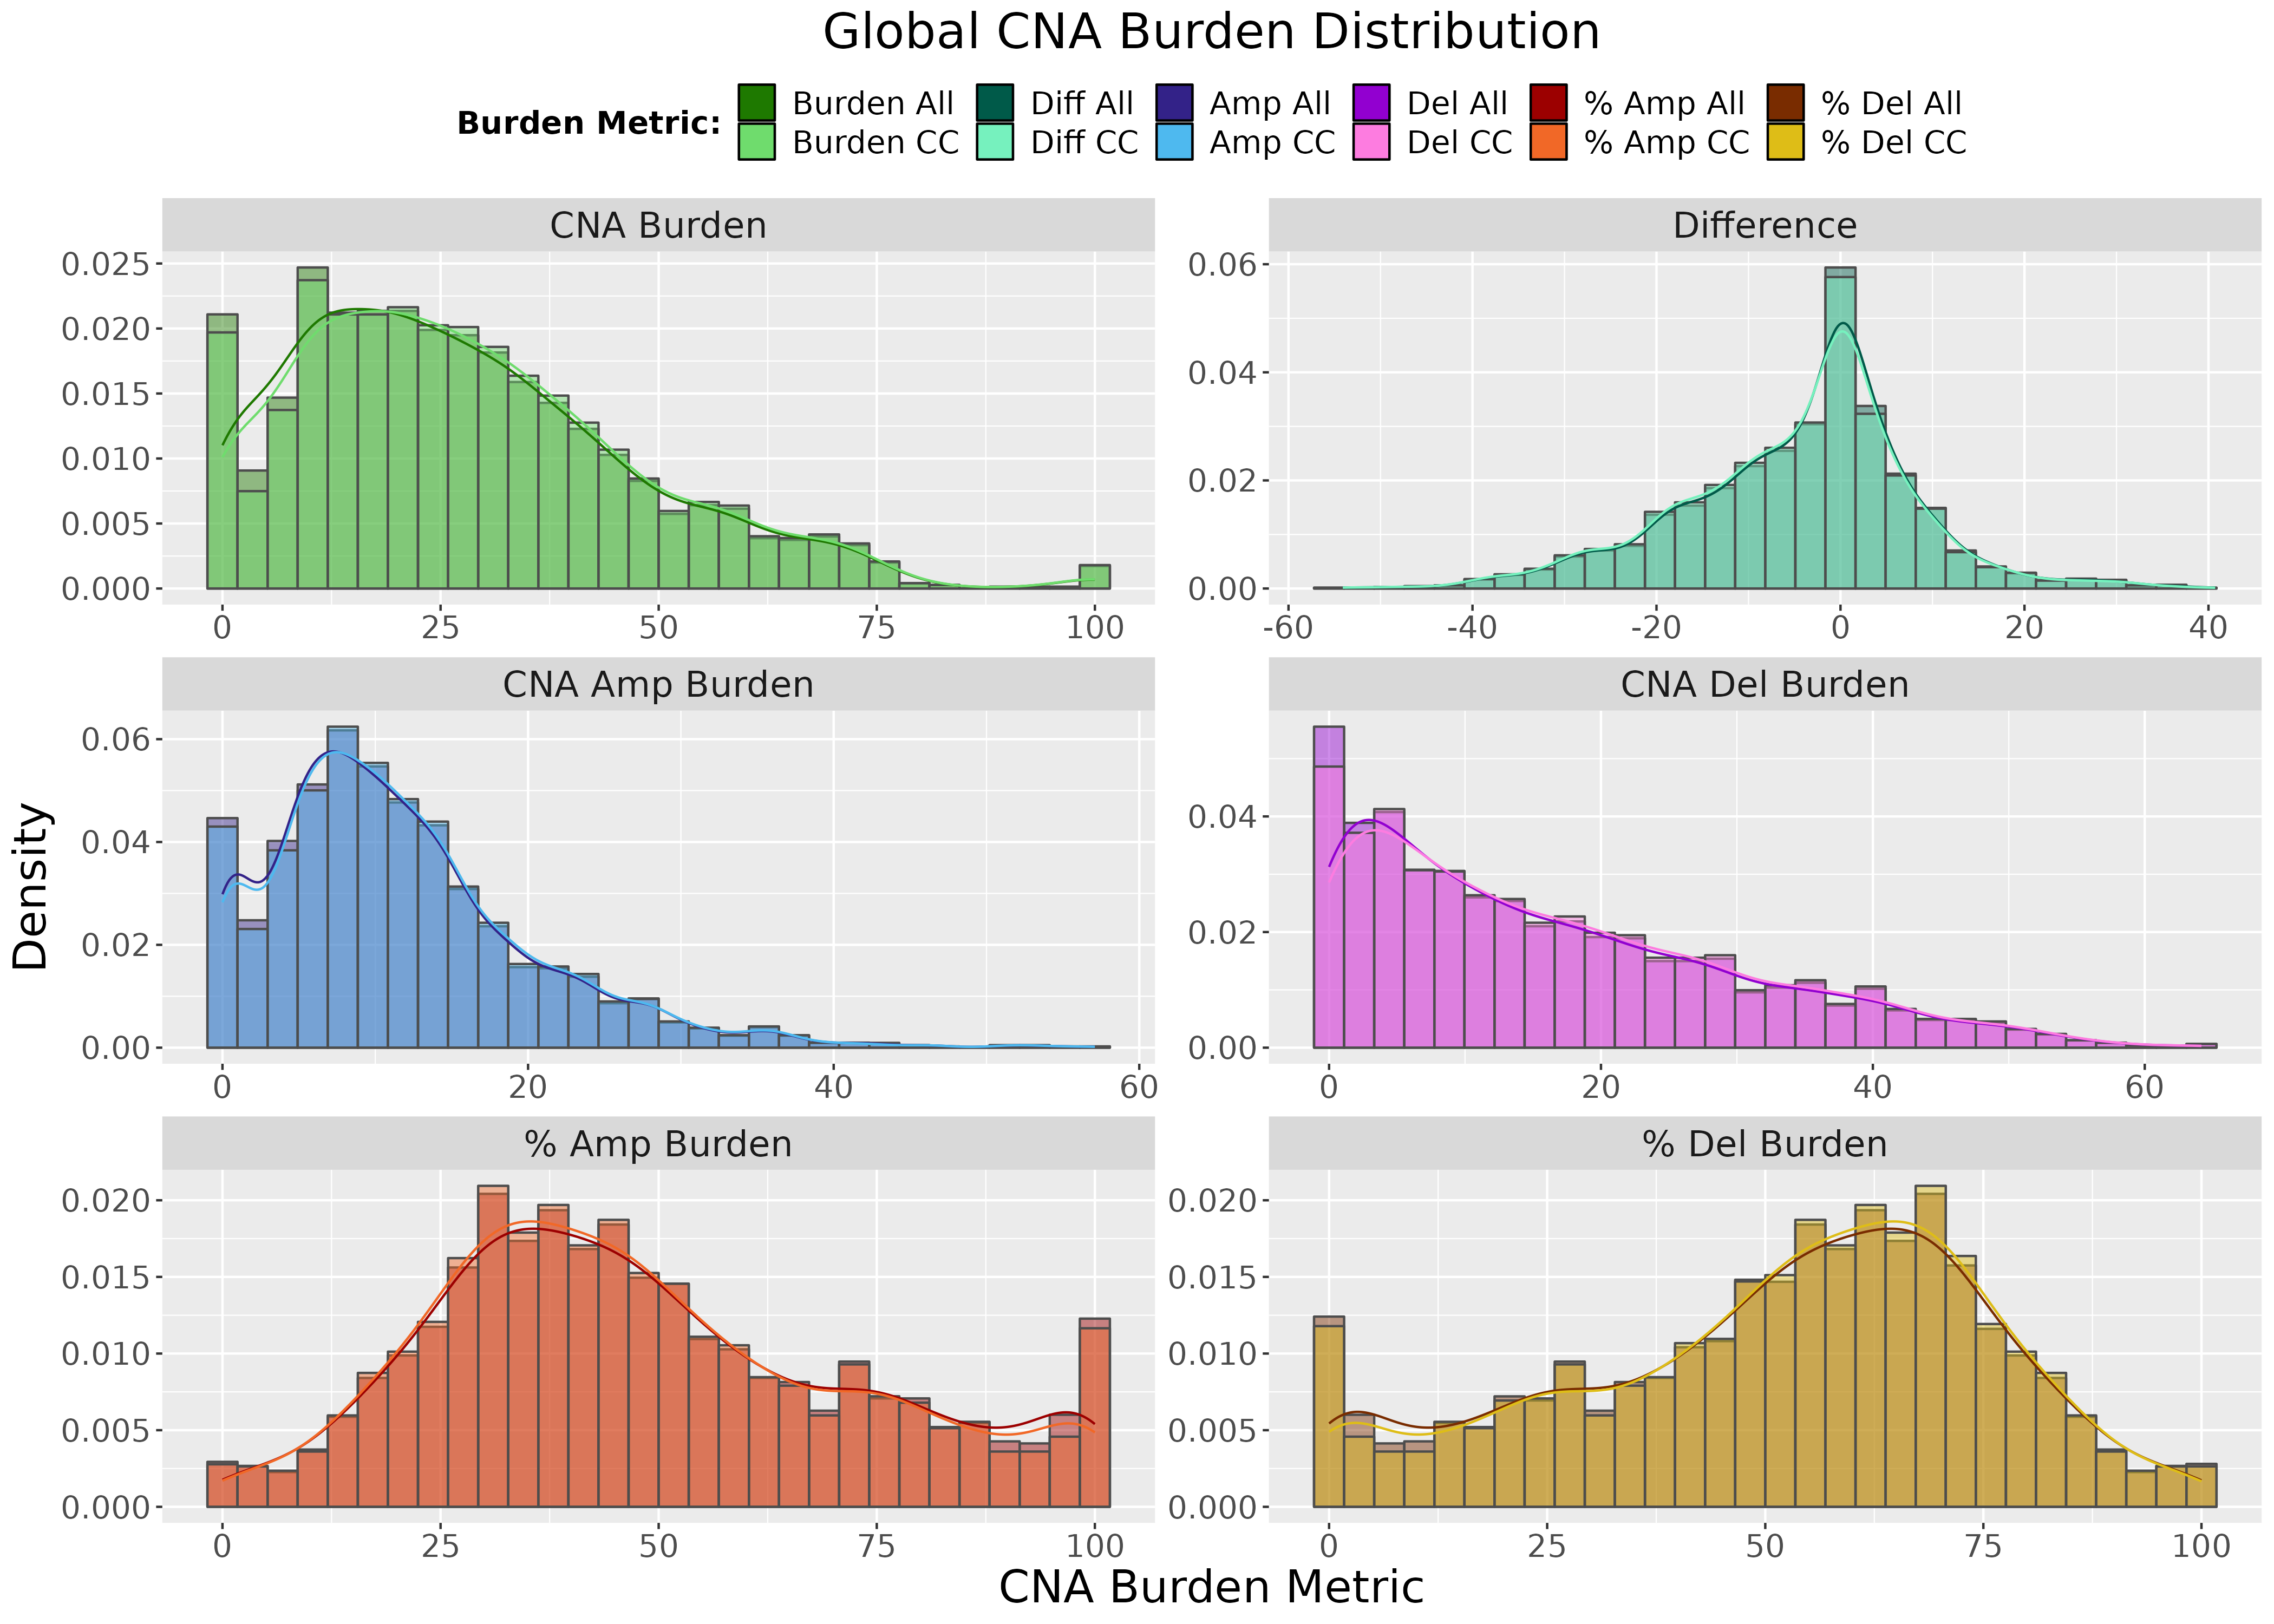
\includegraphics[width = 1\textwidth]{../figures/Chapter_2/Global_CNA_Burden_Comparative_Density.png}
\caption[Density plots for each global CNA Burden metric.]{Density plots for each global CNA Burden metric. Each facet contains density plots for both the complete-case CNA Burden metric and the CNA Burden metric calculated using all available data.}
\label{fig:Burden_Comp_Dense}
\end{figure}

\begin{table}[!htb]
\center
\caption[Summary statistics of the CNA Score metrics where all available data are used.]{Summary statistics of the CNA Score metrics where all available data are used.}
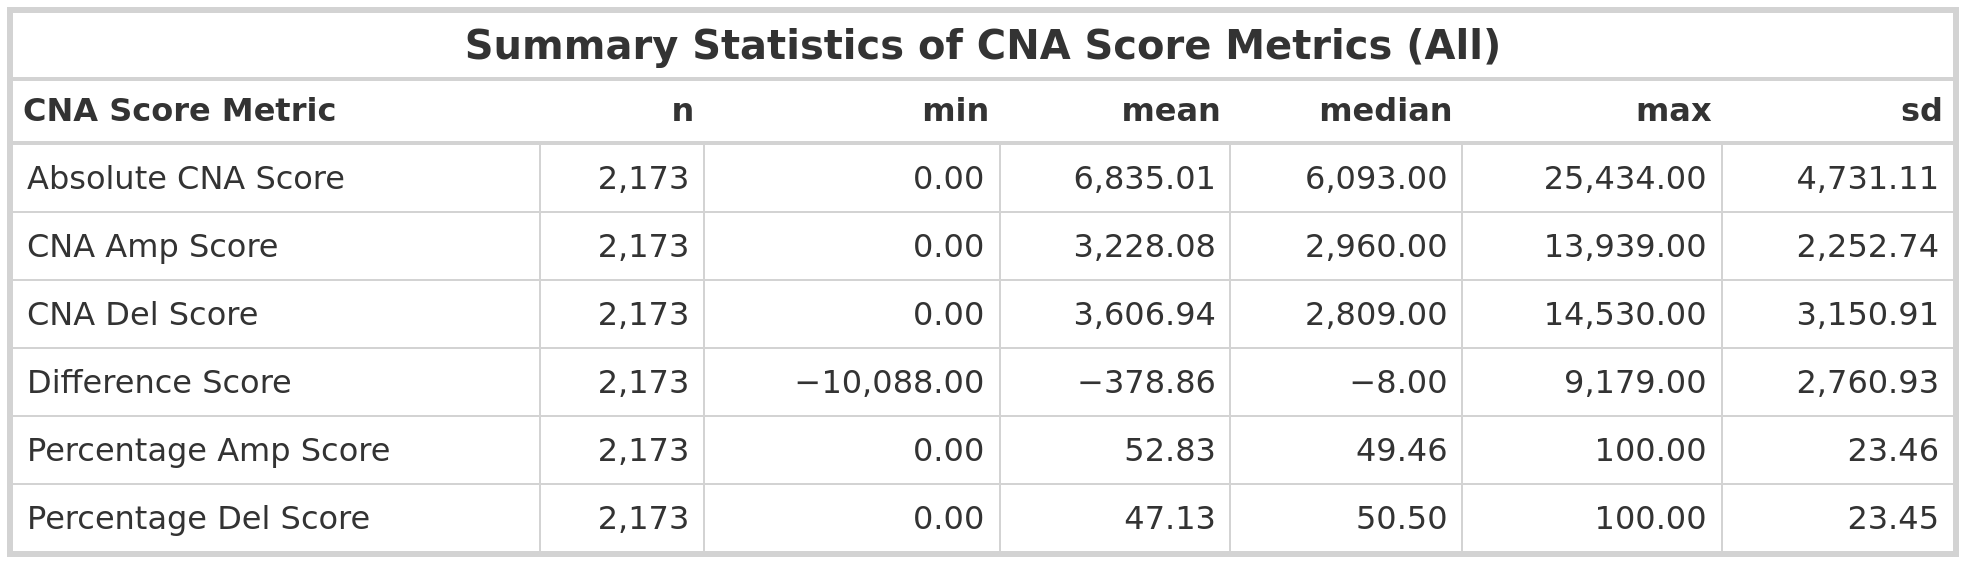
\includegraphics[width = 0.98\textwidth]{../tables/Chapter_2/Global_CNA_Score_Metric_All_Summary.png}
\label{tab:Score_All}
\end{table}

\begin{table}[!htb]
\center
\caption[Summary statistics of the CNA Score metrics where only complete cases are used.]{Summary statistics of the CNA Score metrics where only complete cases are used.}
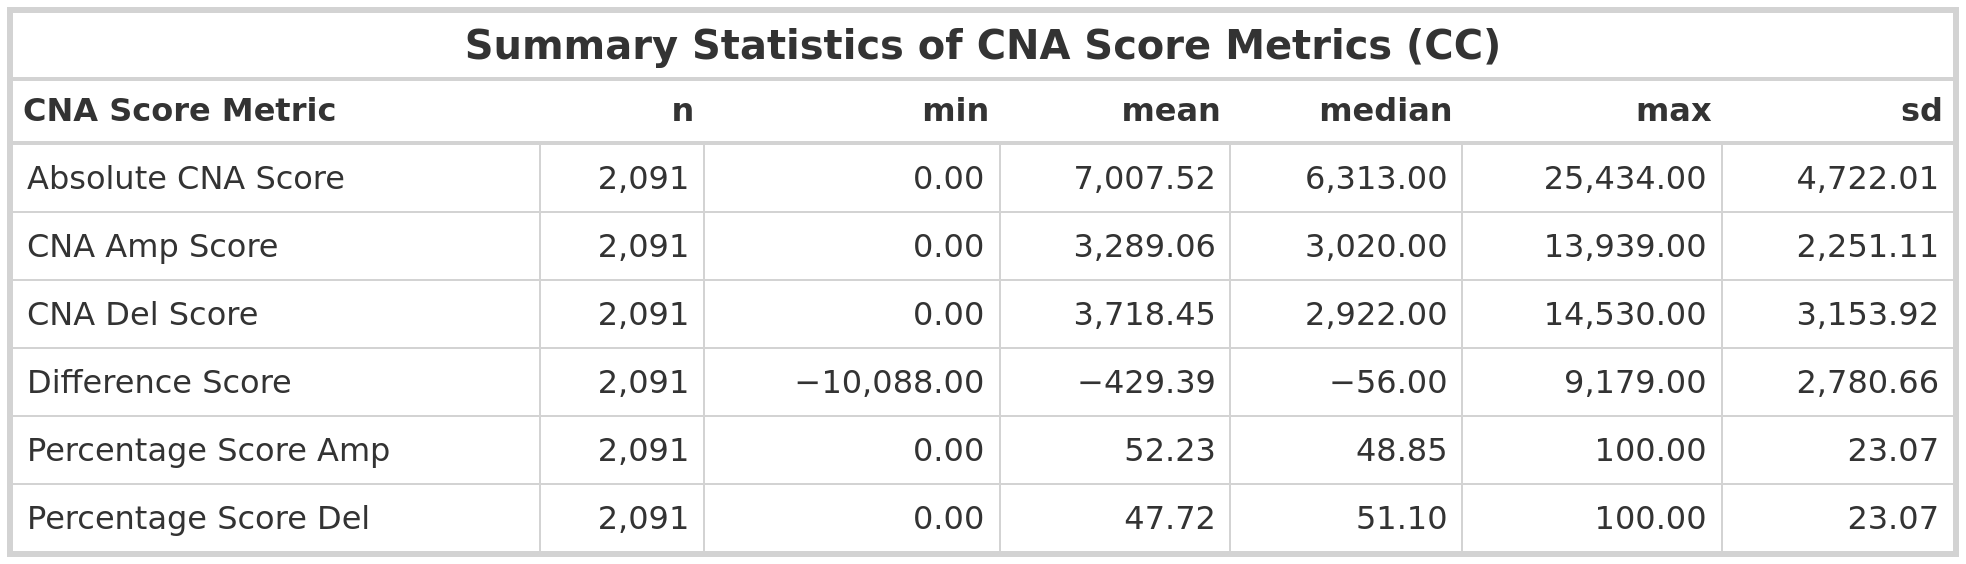
\includegraphics[width = 0.98\textwidth]{../tables/Chapter_2/Global_CNA_Score_Metric_CCA_Summary.png}
\label{tab:Score_CCA}
\end{table}

\begin{table}[!htb]
\center
\caption[Summary statistics of the CNA Burden metrics where all available data are used.]{Summary statistics of the CNA Burden metrics where all available data are used.}
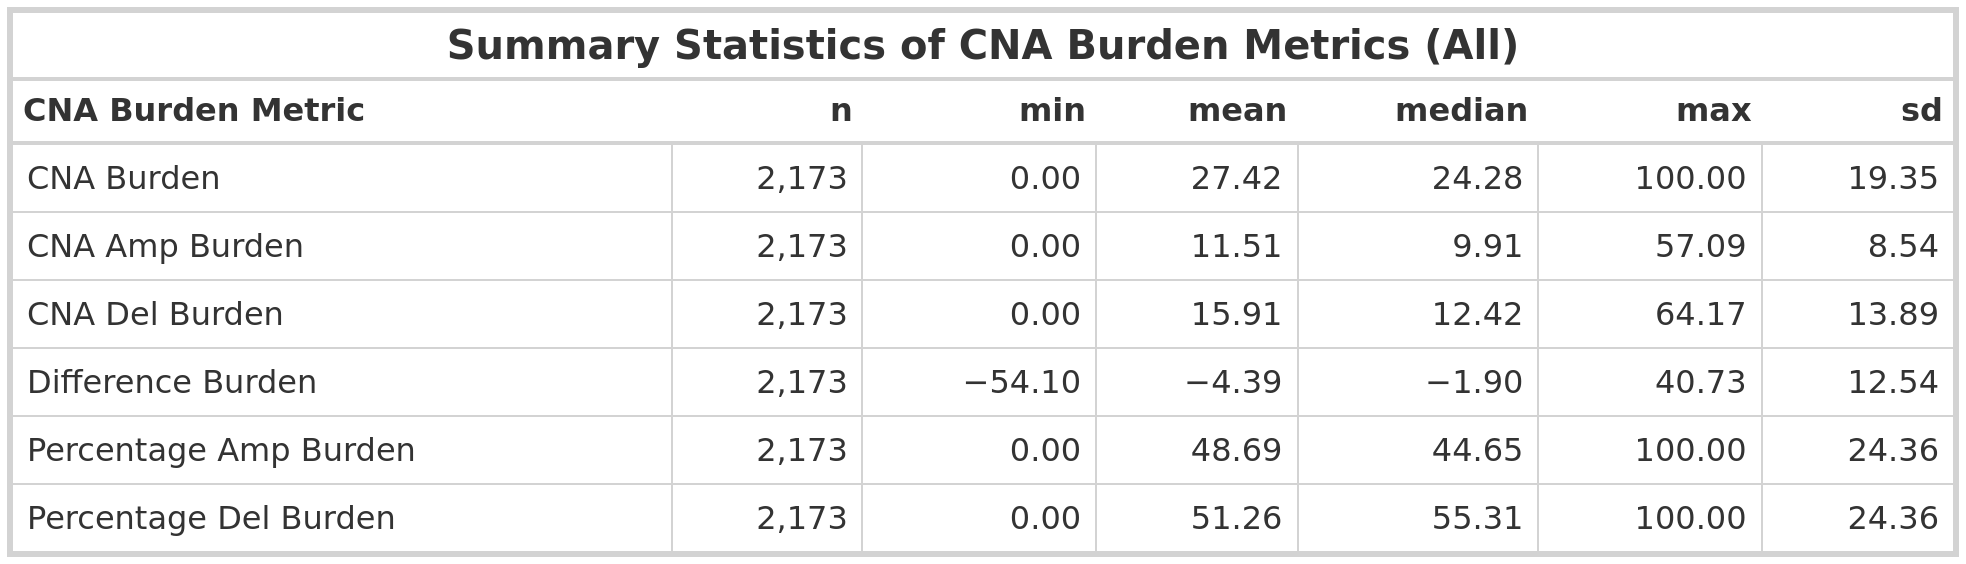
\includegraphics[width = 0.98\textwidth]{../tables/Chapter_2/Global_CNA_Burden_Metric_All_Summary.png}
\label{tab:Burden_All}
\end{table}

\begin{table}[!htb]
\center
\caption[Summary statistics of the CNA Burden metrics where only complete cases are used.]{Summary statistics of the CNA Burden metrics where only complete cases are used.}
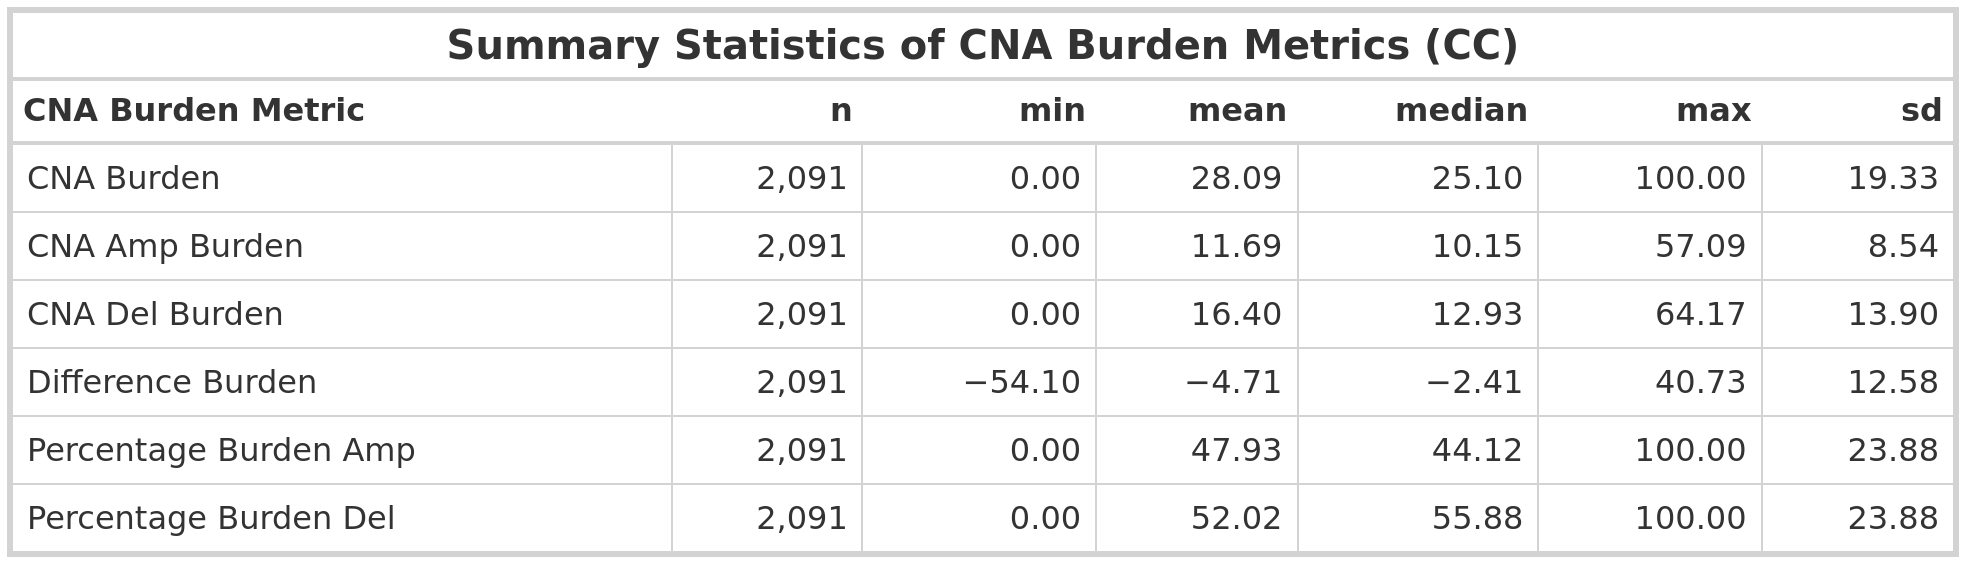
\includegraphics[width = 0.98\textwidth]{../tables/Chapter_2/Global_CNA_Burden_Metric_CCA_Summary.png}
\label{tab:Burden_CCA}
\end{table}

\begin{table}[h]
    \begin{minipage}{.49\linewidth}
    \caption[The percentage overlap between the global complete-case and all-case CNA Score metric densities.]{
    The percentage overlap between the global complete-case and all-case CNA Score metric densities.
    Metrics are ordered and coloured by percentage overlap.}
      \centering 
\begin{tabular}[t]{l>{}r}
\toprule
CNA Score Metric & \% Overlap\\
\midrule
Absolute CNA Score & \cellcolor[HTML]{414487}{\textcolor{white}{96.55}}\\
 
CNA Del Score & \cellcolor[HTML]{482374}{\textcolor{white}{97.15}}\\
 
CNA Amp Score & \cellcolor[HTML]{481769}{\textcolor{white}{97.35}}\\
 
\% CNA Score Amp & \cellcolor[HTML]{46085B}{\textcolor{white}{97.58}}\\
 
\% CNA Score Del & \cellcolor[HTML]{440154}{\textcolor{white}{97.69}}\\
 
Difference Score & \cellcolor[HTML]{440154}{\textcolor{white}{97.69}}\\
\bottomrule
\end{tabular} \label{table:CNAScoreT1}
    \end{minipage}%
    \hspace{0.4cm}
    \begin{minipage}{.49\linewidth}
      \centering
    \caption[The percentage overlap between the global complete-case and all-case CNA Burden metric densities.]{
    The percentage overlap between the global complete-case and all-case CNA Burden metric densities.
    Metrics are ordered and coloured by percentage overlap.} 
\begin{tabular}[t]{l>{}r}
\toprule
CNA Burden Metric & \% Overlap\\
\midrule
CNA Burden & \cellcolor[HTML]{414487}{\textcolor{white}{96.76}}\\
 
CNA Del Burden & \cellcolor[HTML]{472D7B}{\textcolor{white}{97.18}}\\
 
CNA Amp Burden & \cellcolor[HTML]{482979}{\textcolor{white}{97.24}}\\
 
\% CNA Burden Amp & \cellcolor[HTML]{481C6E}{\textcolor{white}{97.45}}\\
 
\% CNA Burden Del & \cellcolor[HTML]{481C6E}{\textcolor{white}{97.45}}\\
 
Difference Burden & \cellcolor[HTML]{440154}{\textcolor{white}{97.87}}\\
\bottomrule
\end{tabular} \label{table:CNABurdenT1}
    \end{minipage}
\end{table}
\clearpage

\subsubsection{Observed Distributions for Chromosome Arm CNA Metrics}  
Similarly, the observed distributions for the chromosome arm CNA metrics are inspected and an assessment of the effects of missingness is carried out. Figures \ref{SurvTrees_Score_HM_CCA} and \ref{SurvTrees_Score_HM} display the heatmaps of the chromosome arm CNA Amp and Del Score metrics calculated using compete cases only and all available data, the grey indicates missing data. Figures \ref{SurvTrees_Burden_HM_CCA} and \ref{SurvTrees_Burden_HM} display the heatmaps of the chromosome arm CNA Amp and Del Burden metrics calculated using compete cases only and all available data. Comparing A and B in each of these figures, it is observed that similar clusters of patients are generated based on both the all-case and CC chromosome arm CNA metrics. When comparing the overlap in distributions it is observed that only 10 out of the 252 chromosome arm CNA Score and Burden metrics display percentage overlap below 80\%. The lowest overlap in the CNA Score and Burden metric distributions is in the Percentage Amp metrics on 9p, 11.00\% and 10.84\%, respectively (Table \ref{table:CNAScoreT2} and \ref{table:CNABurdenT2}). The second and third lowest overlap between the CC and all-case CNA Score and Burden metric distributions is observed for chromosome arms 9p, 16.69\% and 16.83\%, and 7p, 42.65\% and 45.26\%. Density plots, focusing on chromosome 9p and 7p, are provided in Figure \ref{fig:Plot-PerArm-DensityPlots} and indicate that high density regions, such as those located around 0, display high levels of mismatch.  

Figures \ref{SurvTrees_Score_HM_CCA}-\ref{SurvTrees_Burden_HM} also highlight previously documented patterns of CNAs in breast cancer, including high levels of amplifications on chromosome 1q, 8q and 16p and high levels of deletions on 8p, 16q and 17p \citep{pmid20576095, pmid22522925}. Similar to the global CNA Score and Burden metrics, it appears that deletions are more widespread across the genome, affecting greater numbers of chromosomes, than amplifications. 

Rather than extensively presenting details of distributions for each of the 42 chromosome arms, we select chromosome arm 1q for more detailed illustration and discussion (see online Supplementary Information for remaining chromosome arms). Chromosome arm 1q is frequently altered in breast cancer and shows interesting features in this analysis. The summary statistics (Tables \ref{tab:Score_All_Chr1q}-\ref{tab:Burden_CCA_Chr1q}) and distributions (Figures \ref{fig:Score_Comp_Dense_Chr1q} and \ref{fig:Burden_Comp_Dense_Chr1q}) indicate that the copy number landscape of chromosome 1q is dominated by amplifications, median CNA Score values 0 and 954 and median CNA Burden values 0 and 78.71\%, for deletions and amplifications, respectively. The maximum values of the CNA Burden and CNA Amp, 100\% and 99.91\%, and the Difference Score distribution being nearly entirely positive also suggests that almost all of the alterations observed are amplifications. Figure \ref{fig:Score_Comp_Dense_Chr1q} indicates that three of the CNA Score metrics on chromosome 1q, Absolute CNA Score, CNA Amp Score and Difference Score, have trimodal distributions. Three peaks correspond to cases where patients have low, moderate and high levels of GI. For the CNA Burden metrics the majority of the metric distributions are bimodal, with peaks corresponding to patients with low and high GI. 

Overall, assessing distributions of the global CNA metrics comparing CC patient data to all-patient data, i.e. including those with some missingness prevalent, shows that missing values have only a minor impact on these distributions. The impact of missingness is greater in the chromosome arm CNA metric distributions, however, as the majority of distributions displayed greater than 80\% overlap, it is determined that including all cases, across the global and chromosome arm-specific metrics, is unlikely to invoke bias in the form of underestimating the CNA metrics. Furthermore, imputation of missing CNA values was considered but not performed as the impact of the missing values on the CNA metric distributions was shown to be minor across the majority of CNA metrics.

\vfill
\begin{figure}[!h]
  \centering
   \vspace{0.4cm}
  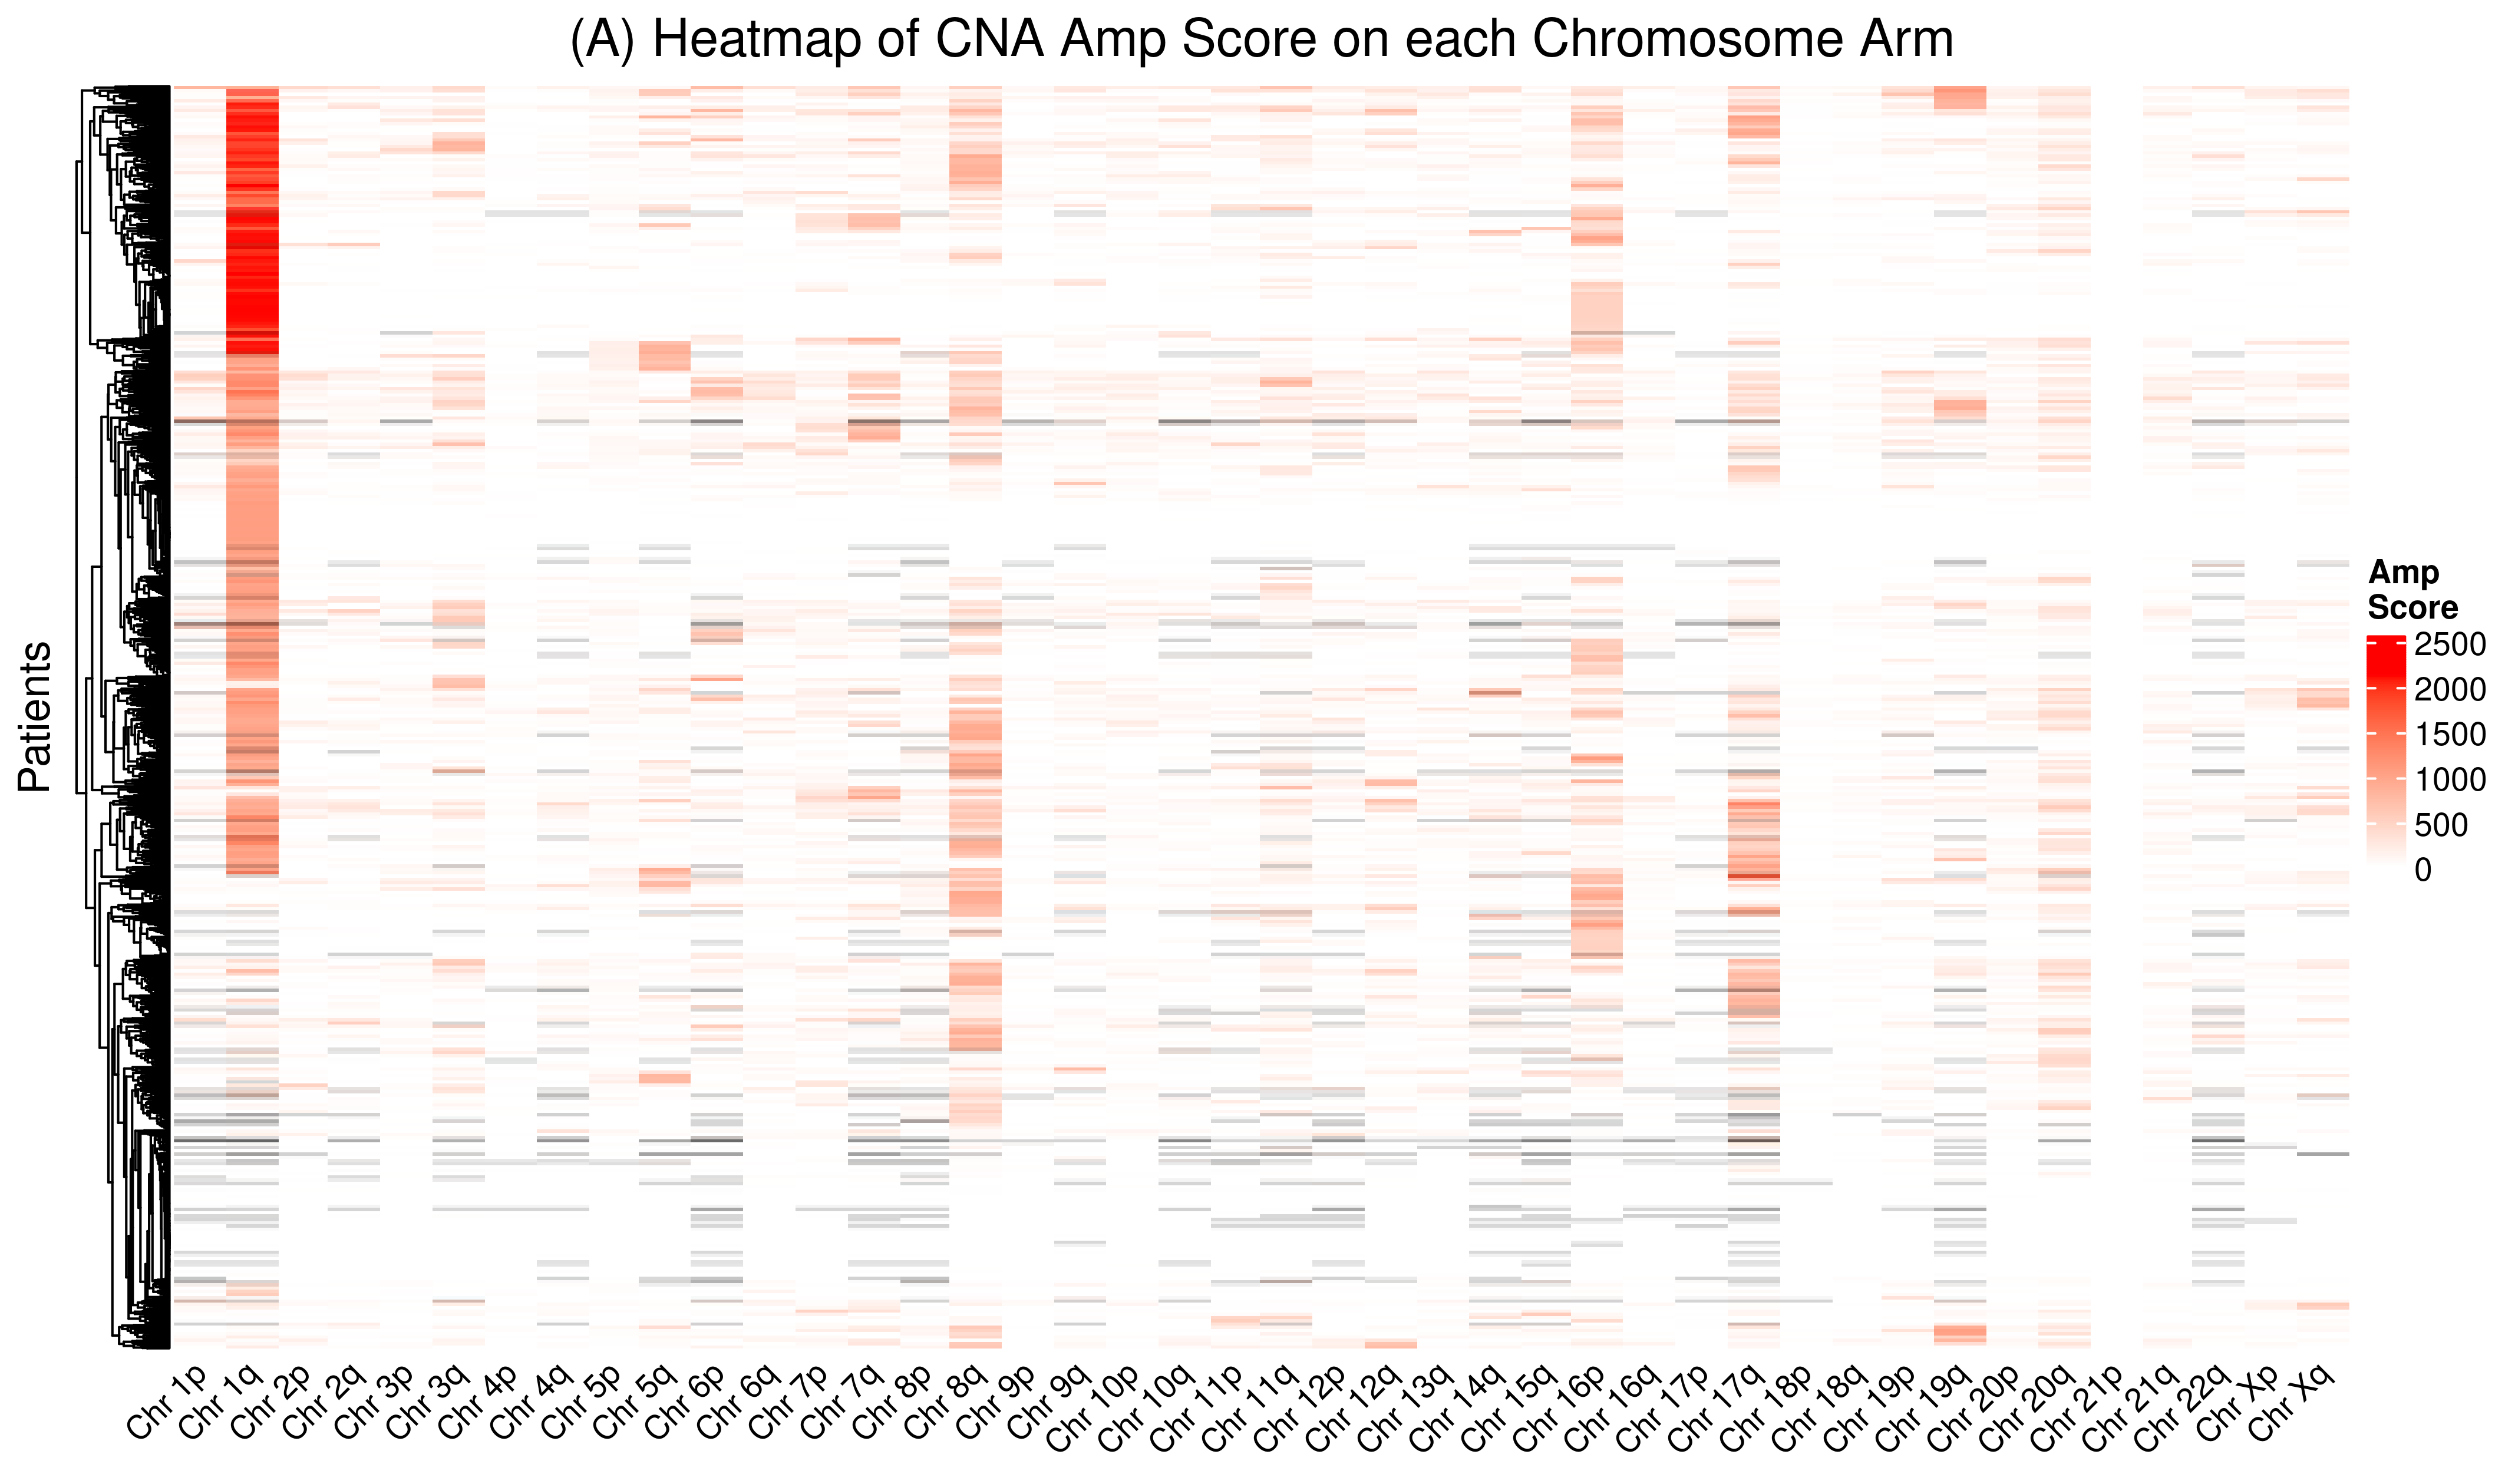
\includegraphics[width = 1.05\textwidth]{../figures/Chapter_2/CNA_Amp_Score_Heatmap_CCA.png}
  
  \vspace{1.3cm}
  
    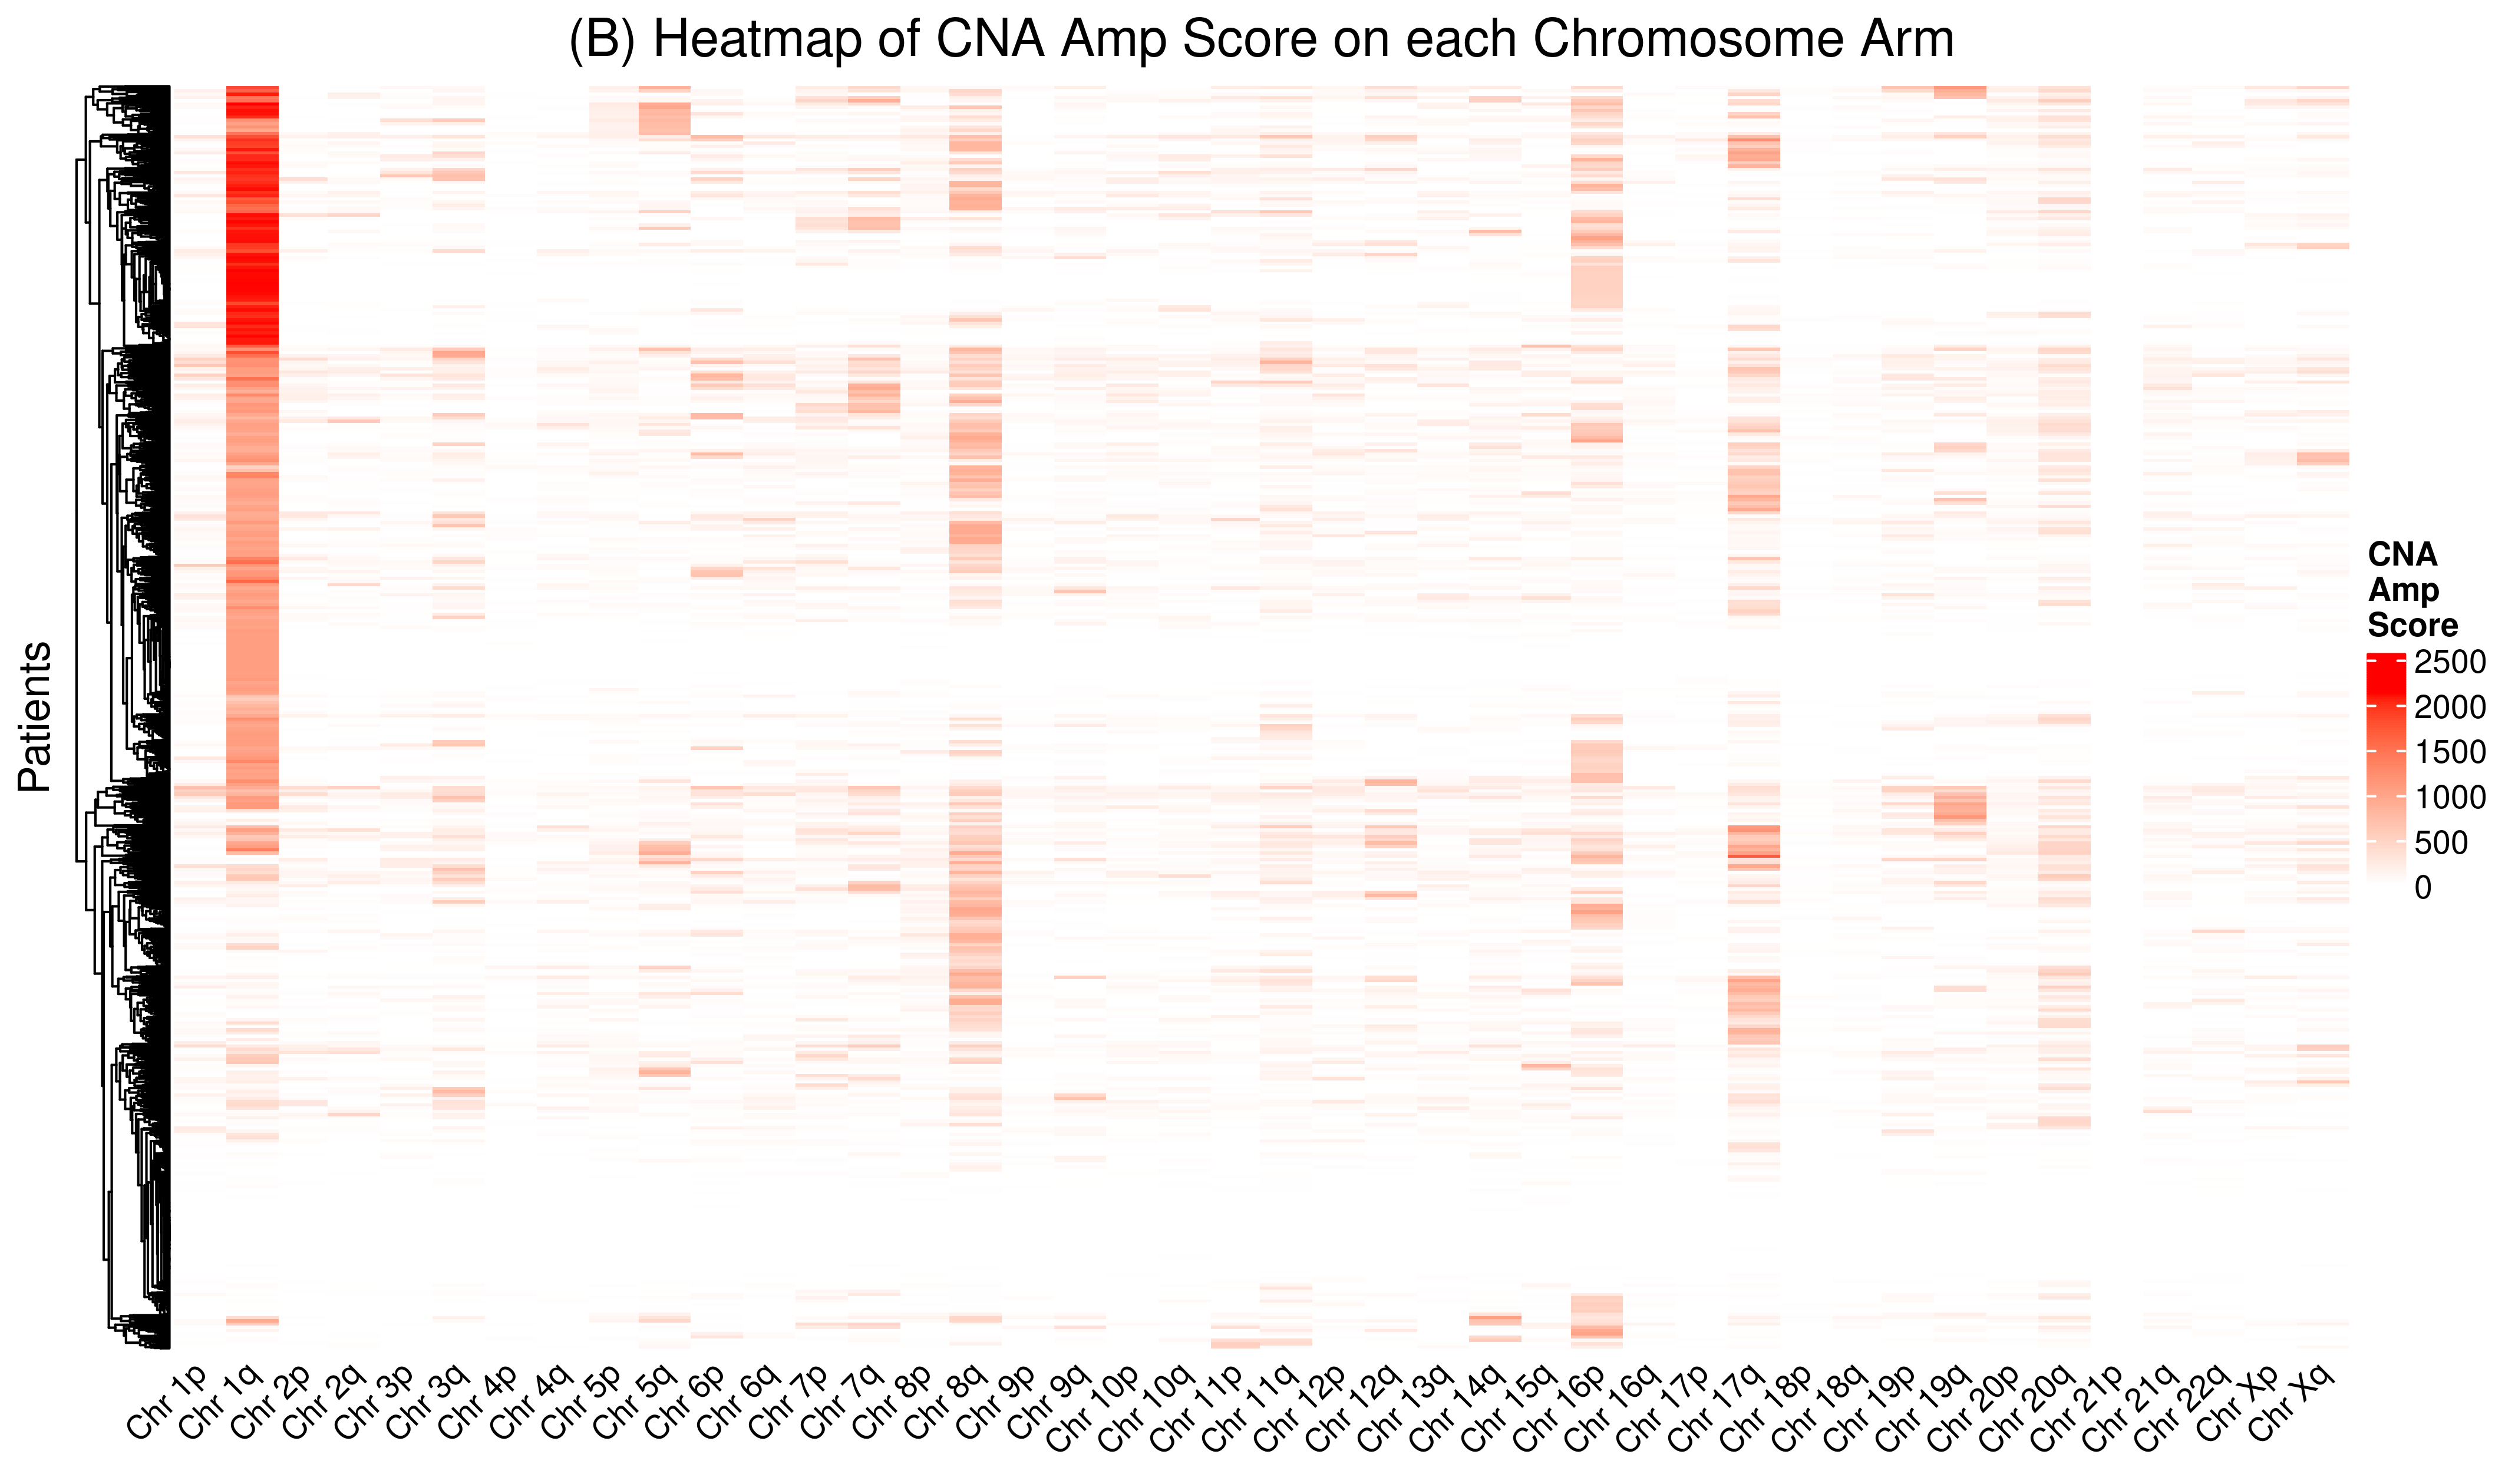
\includegraphics[width = 1.05\textwidth]{../figures/Chapter_2/CNA_Amp_Score_Heatmap_All.png}
  
   \vspace{0.4cm}
 
  \caption[Heatmap of CNA Amp Score across chromosome arms.]{Heatmap of CNA Amp Score across chromosome arms with (A) consideration to complete-case METABRIC patients only (n = 2,091) and (B) consideration to all METABRIC patients including those presenting with some missing data (n = 2,173). Grey indicates missing values.}
  \label{SurvTrees_Score_HM_CCA}
\end{figure}
\vfill 
\clearpage

\begin{figure}[!ht]
  \centering
  
  \vspace{0.8cm}
  
   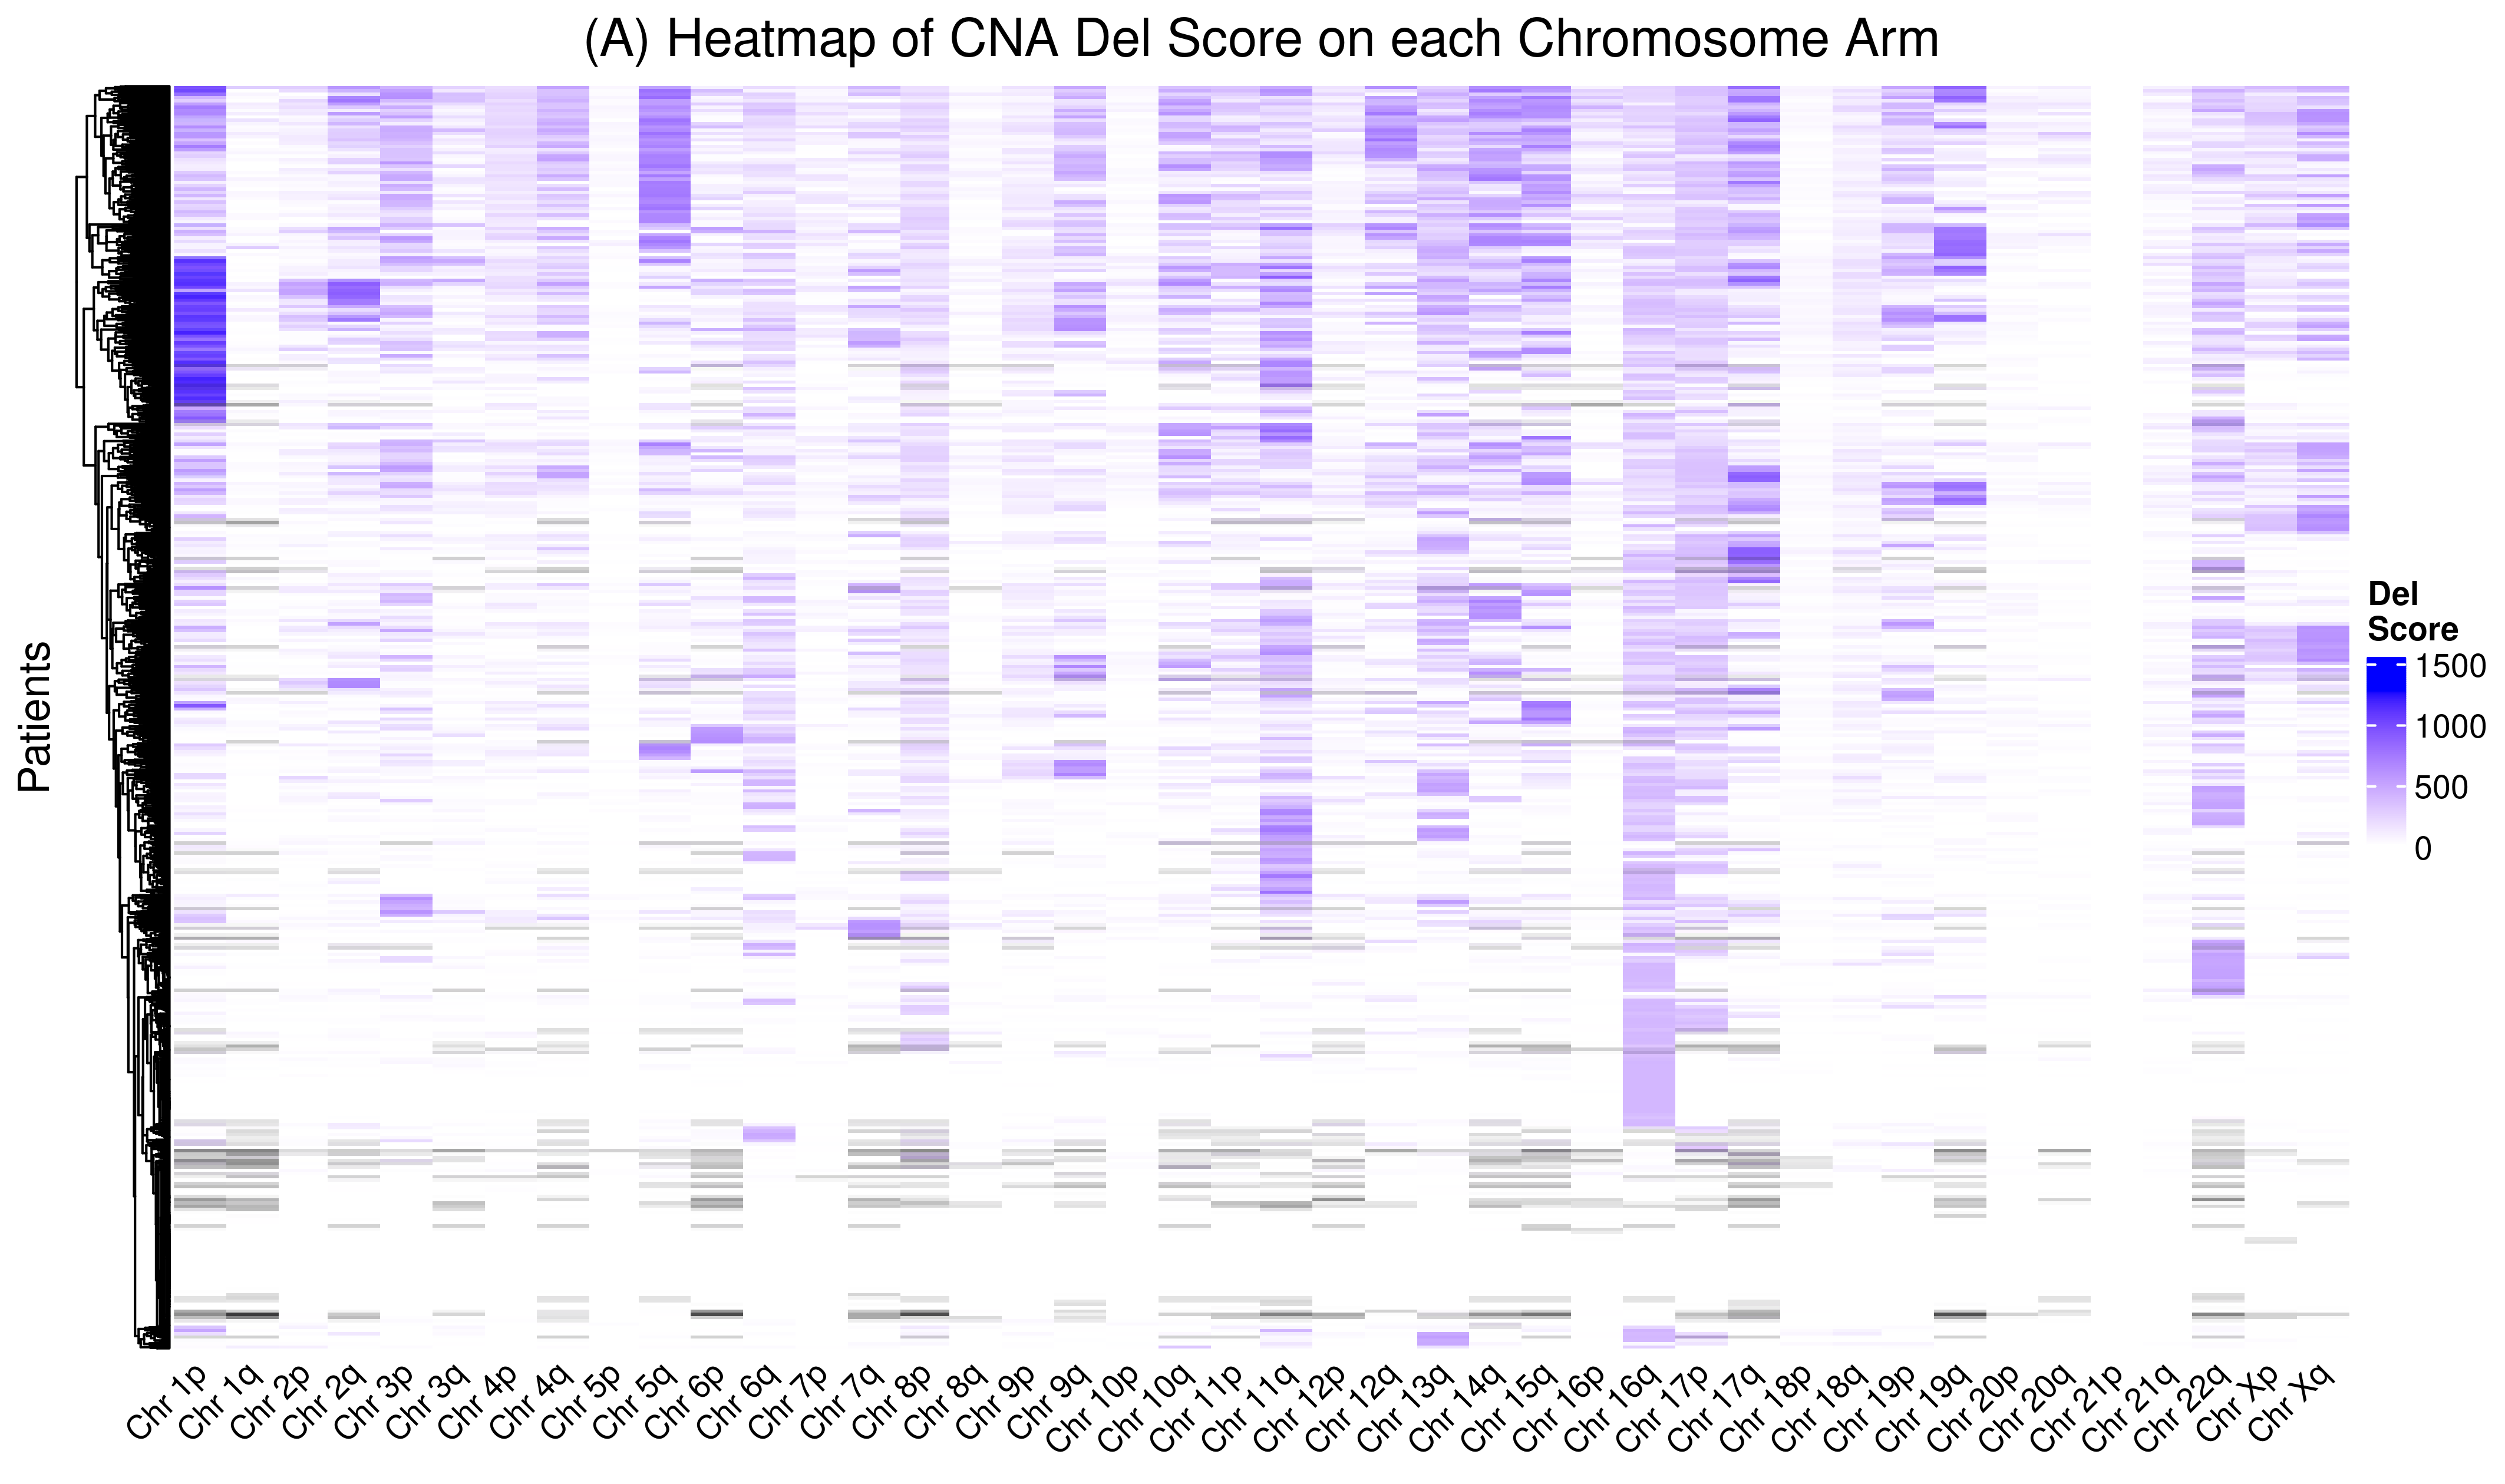
\includegraphics[width = 1.05\textwidth]{../figures/Chapter_2/CNA_Del_Score_Heatmap_CCA.png}

  \vspace{1.5cm}
   
  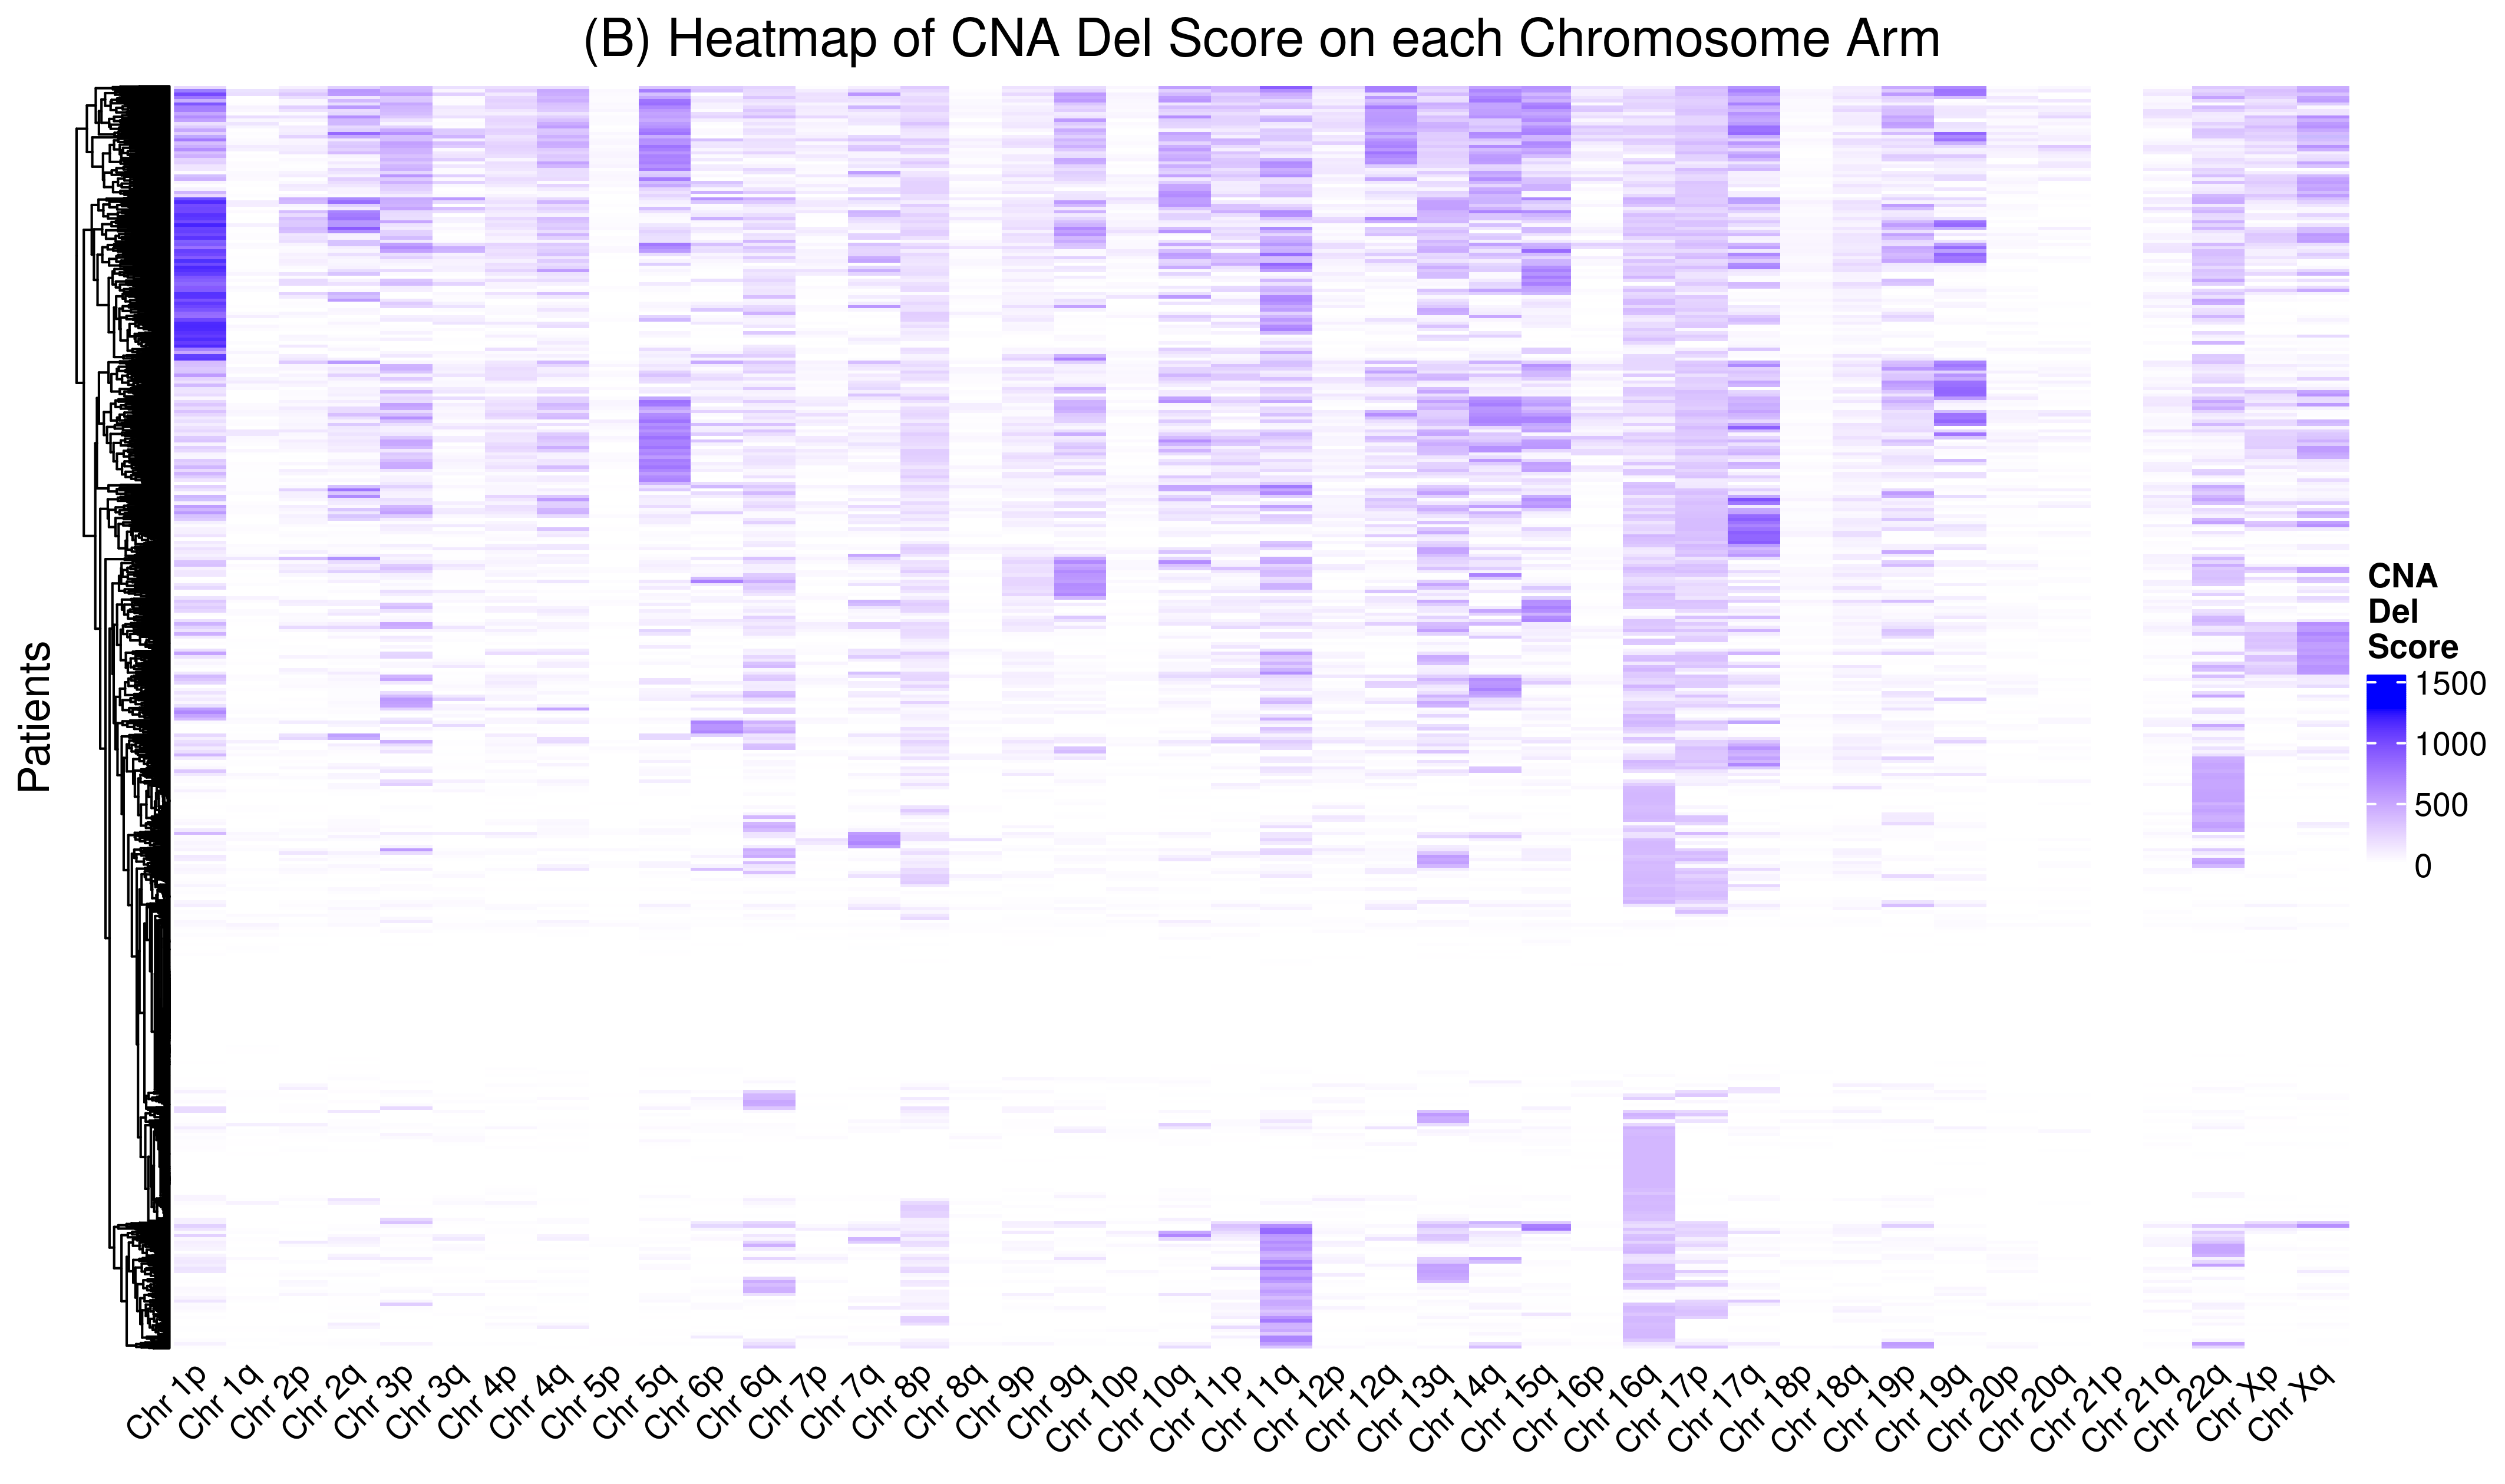
\includegraphics[width = 1.05\textwidth]{../figures/Chapter_2/CNA_Del_Score_Heatmap_All.png}
  
  \vspace{0.8cm}
  
  \caption[Heatmap of CNA Del Score across chromosome arms.]{Heatmap of CNA Del Score across chromosome arms with (A) consideration to complete-case METABRIC patients only (n = 2,091) and (B) consideration to all METABRIC patients including those presenting with some missing data (n = 2,173). Grey indicates missing values.}
  \label{SurvTrees_Score_HM}
\end{figure}
\clearpage

\begin{figure}[!ht]
  \centering
  
  \vspace{0.8cm}
  
  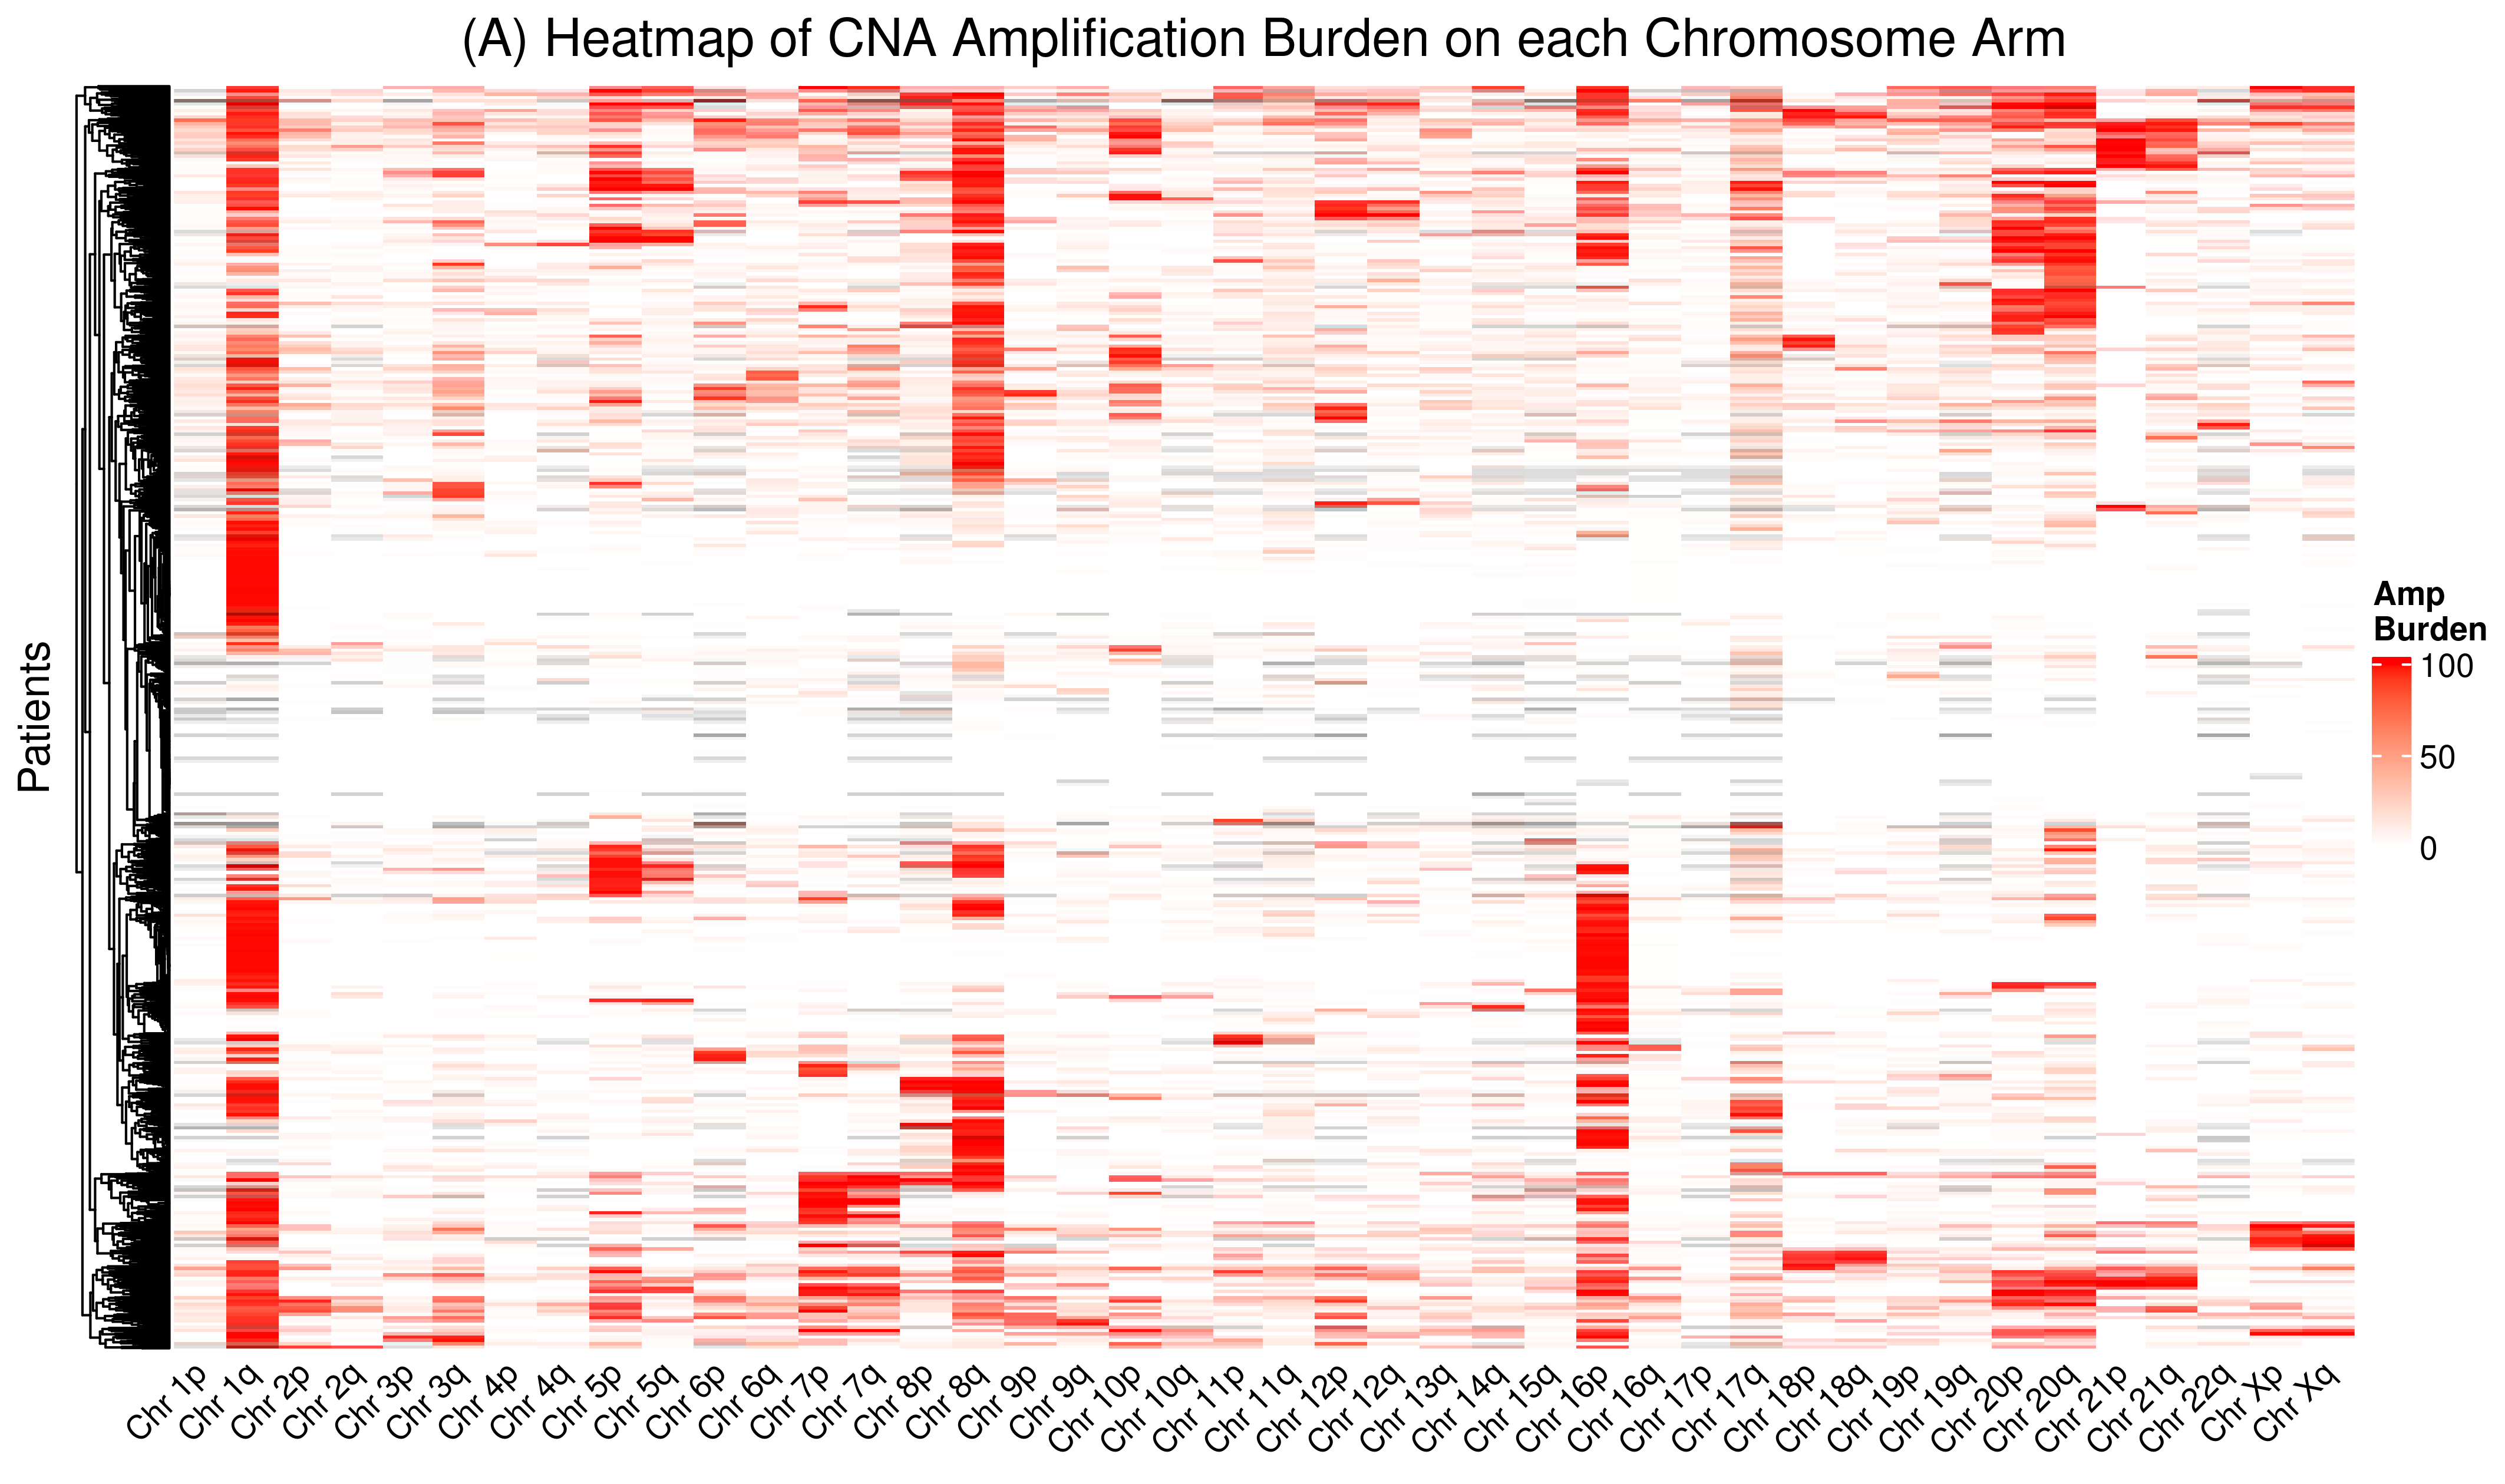
\includegraphics[width = 1.05\textwidth]{../figures/Chapter_2/CNA_Amp_Burden_Heatmap_CCA.png}
  
  \vspace{1.5cm}
  
     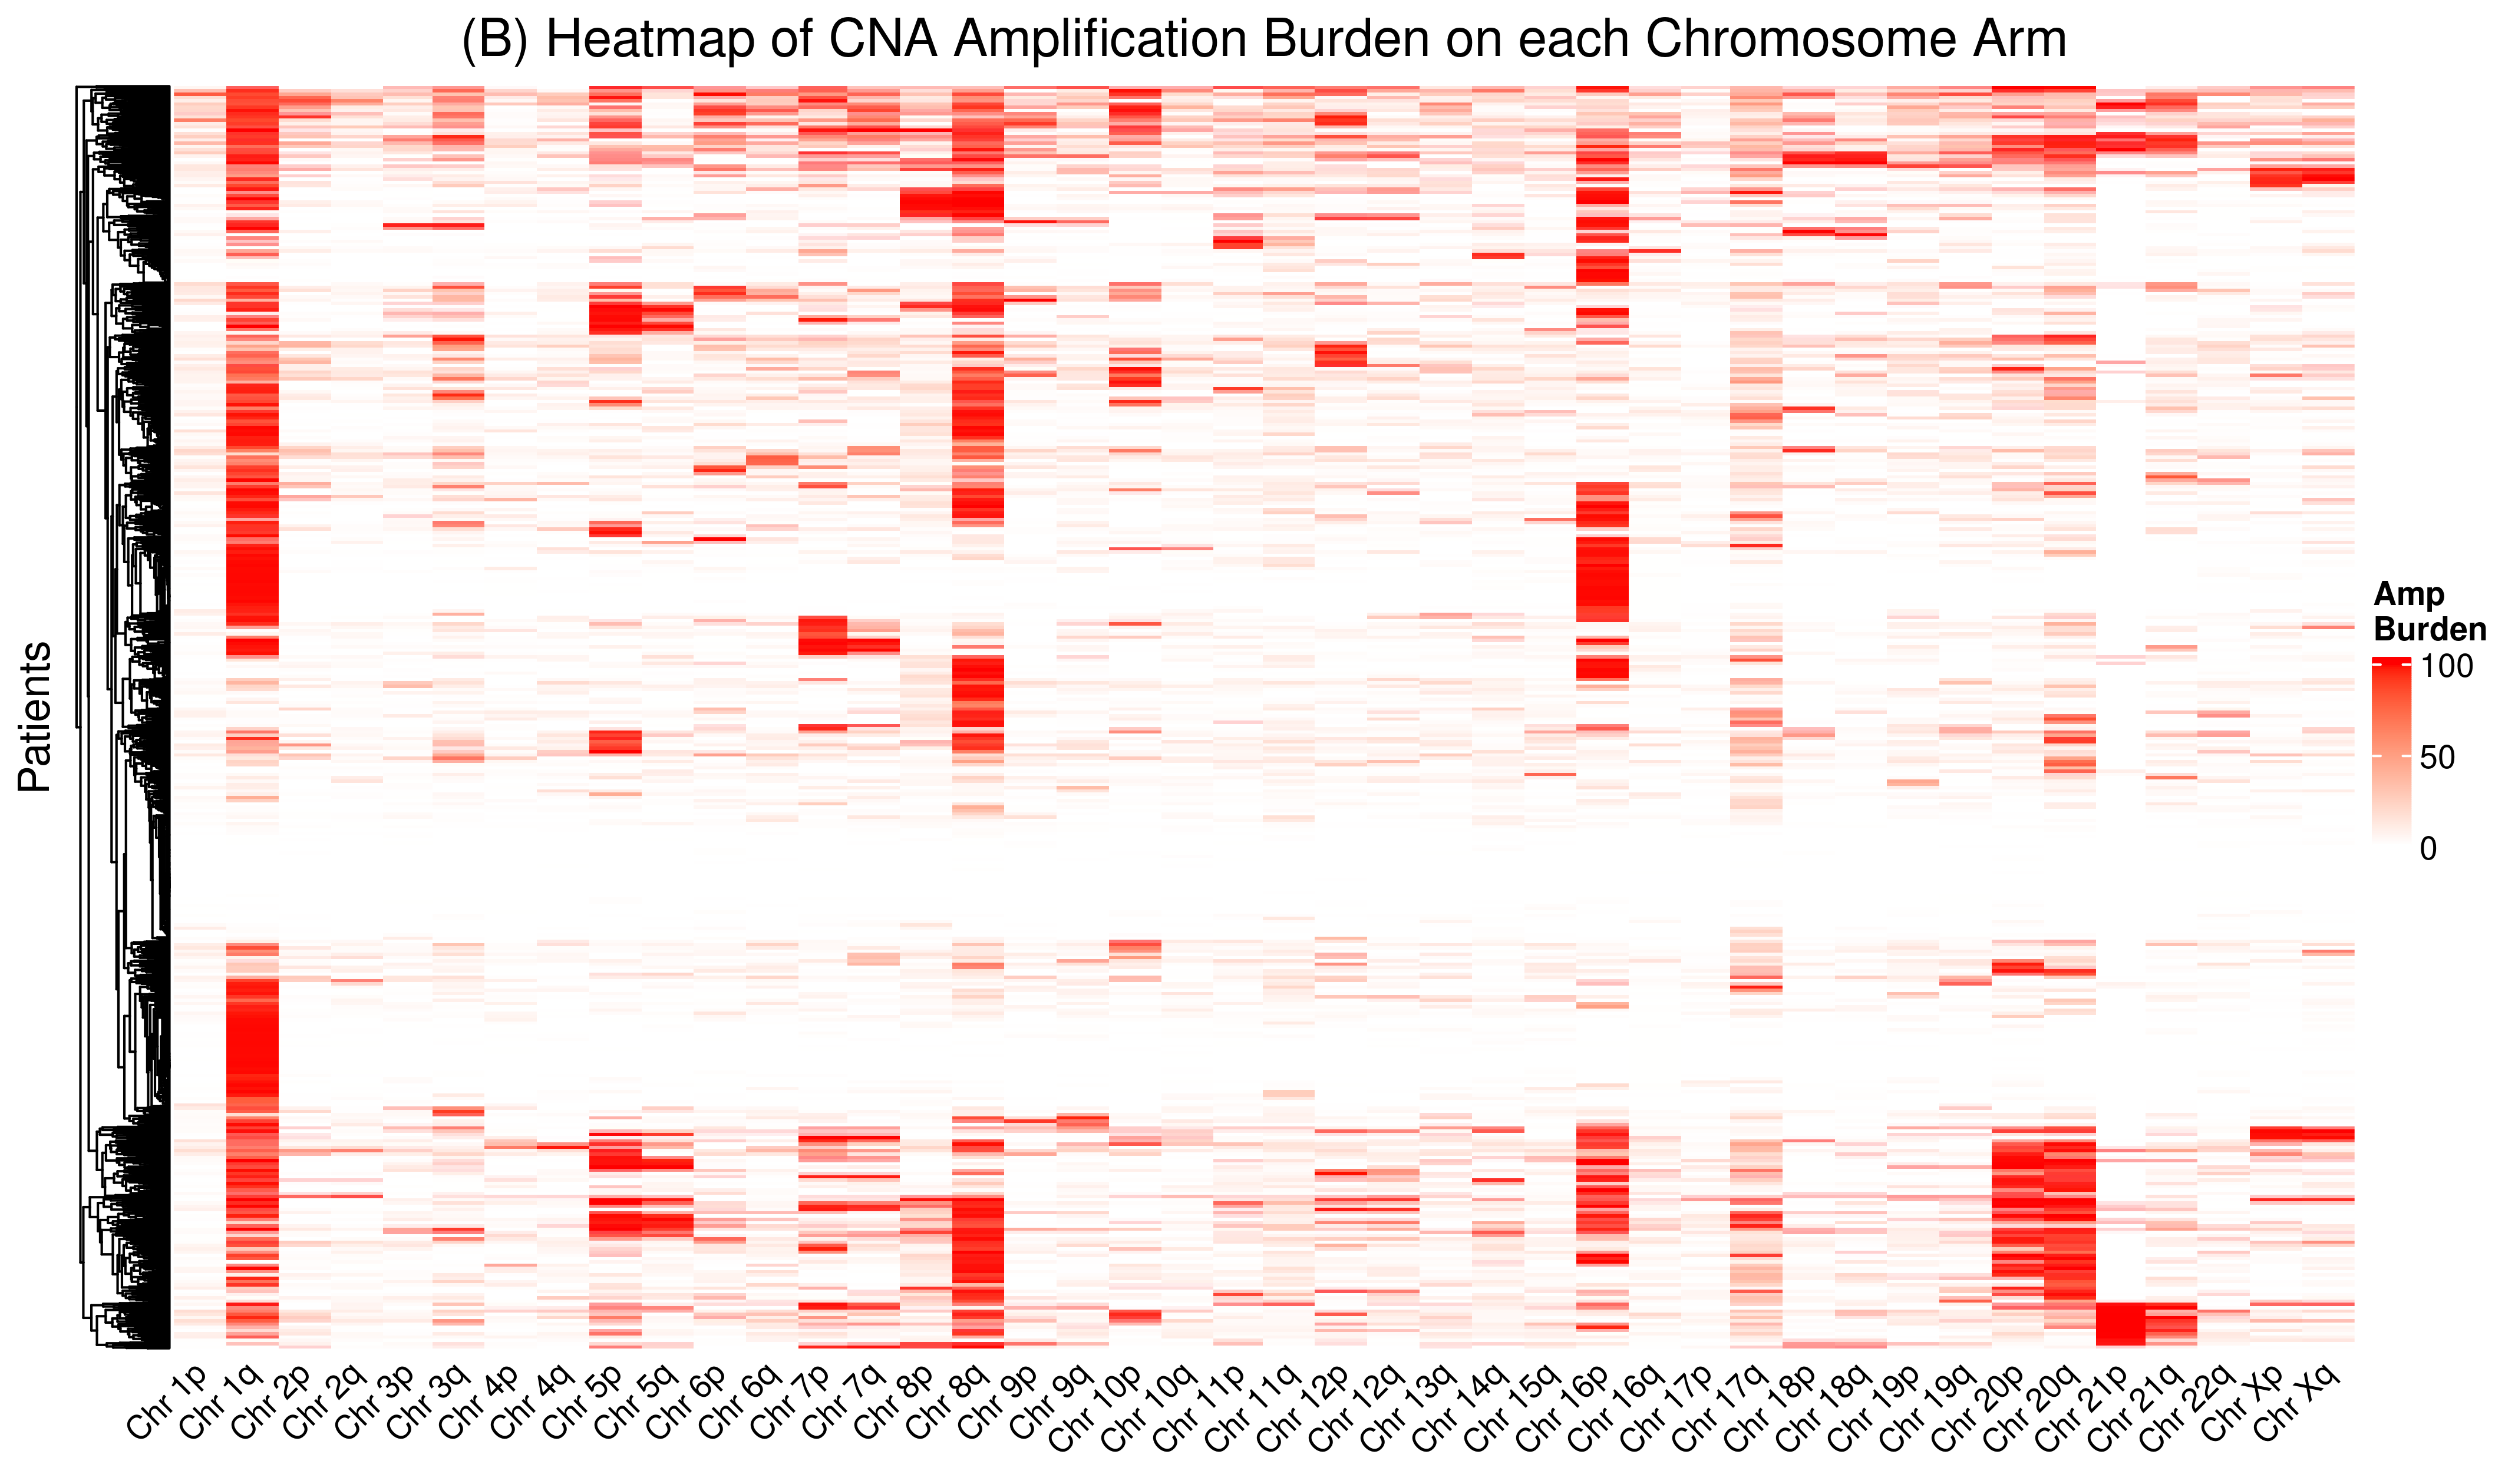
\includegraphics[width = 1.05\textwidth]{../figures/Chapter_2/CNA_Amp_Burden_Heatmap_All.png} 

\vspace{0.8cm}

  \caption[Heatmap of CNA Amp Burden across chromosome arms.]{Heatmap of CNA Amp Burden across chromosome arms with (A) consideration to complete-case METABRIC patients only (n = 2,091) and (B) consideration to all METABRIC patients including those presenting with some missing data (n = 2,173). Grey indicates missing values.}
  \label{SurvTrees_Burden_HM_CCA}
\end{figure}
\clearpage

\begin{figure}[!ht]
  \centering
  
  \vspace{0.8cm}
  
    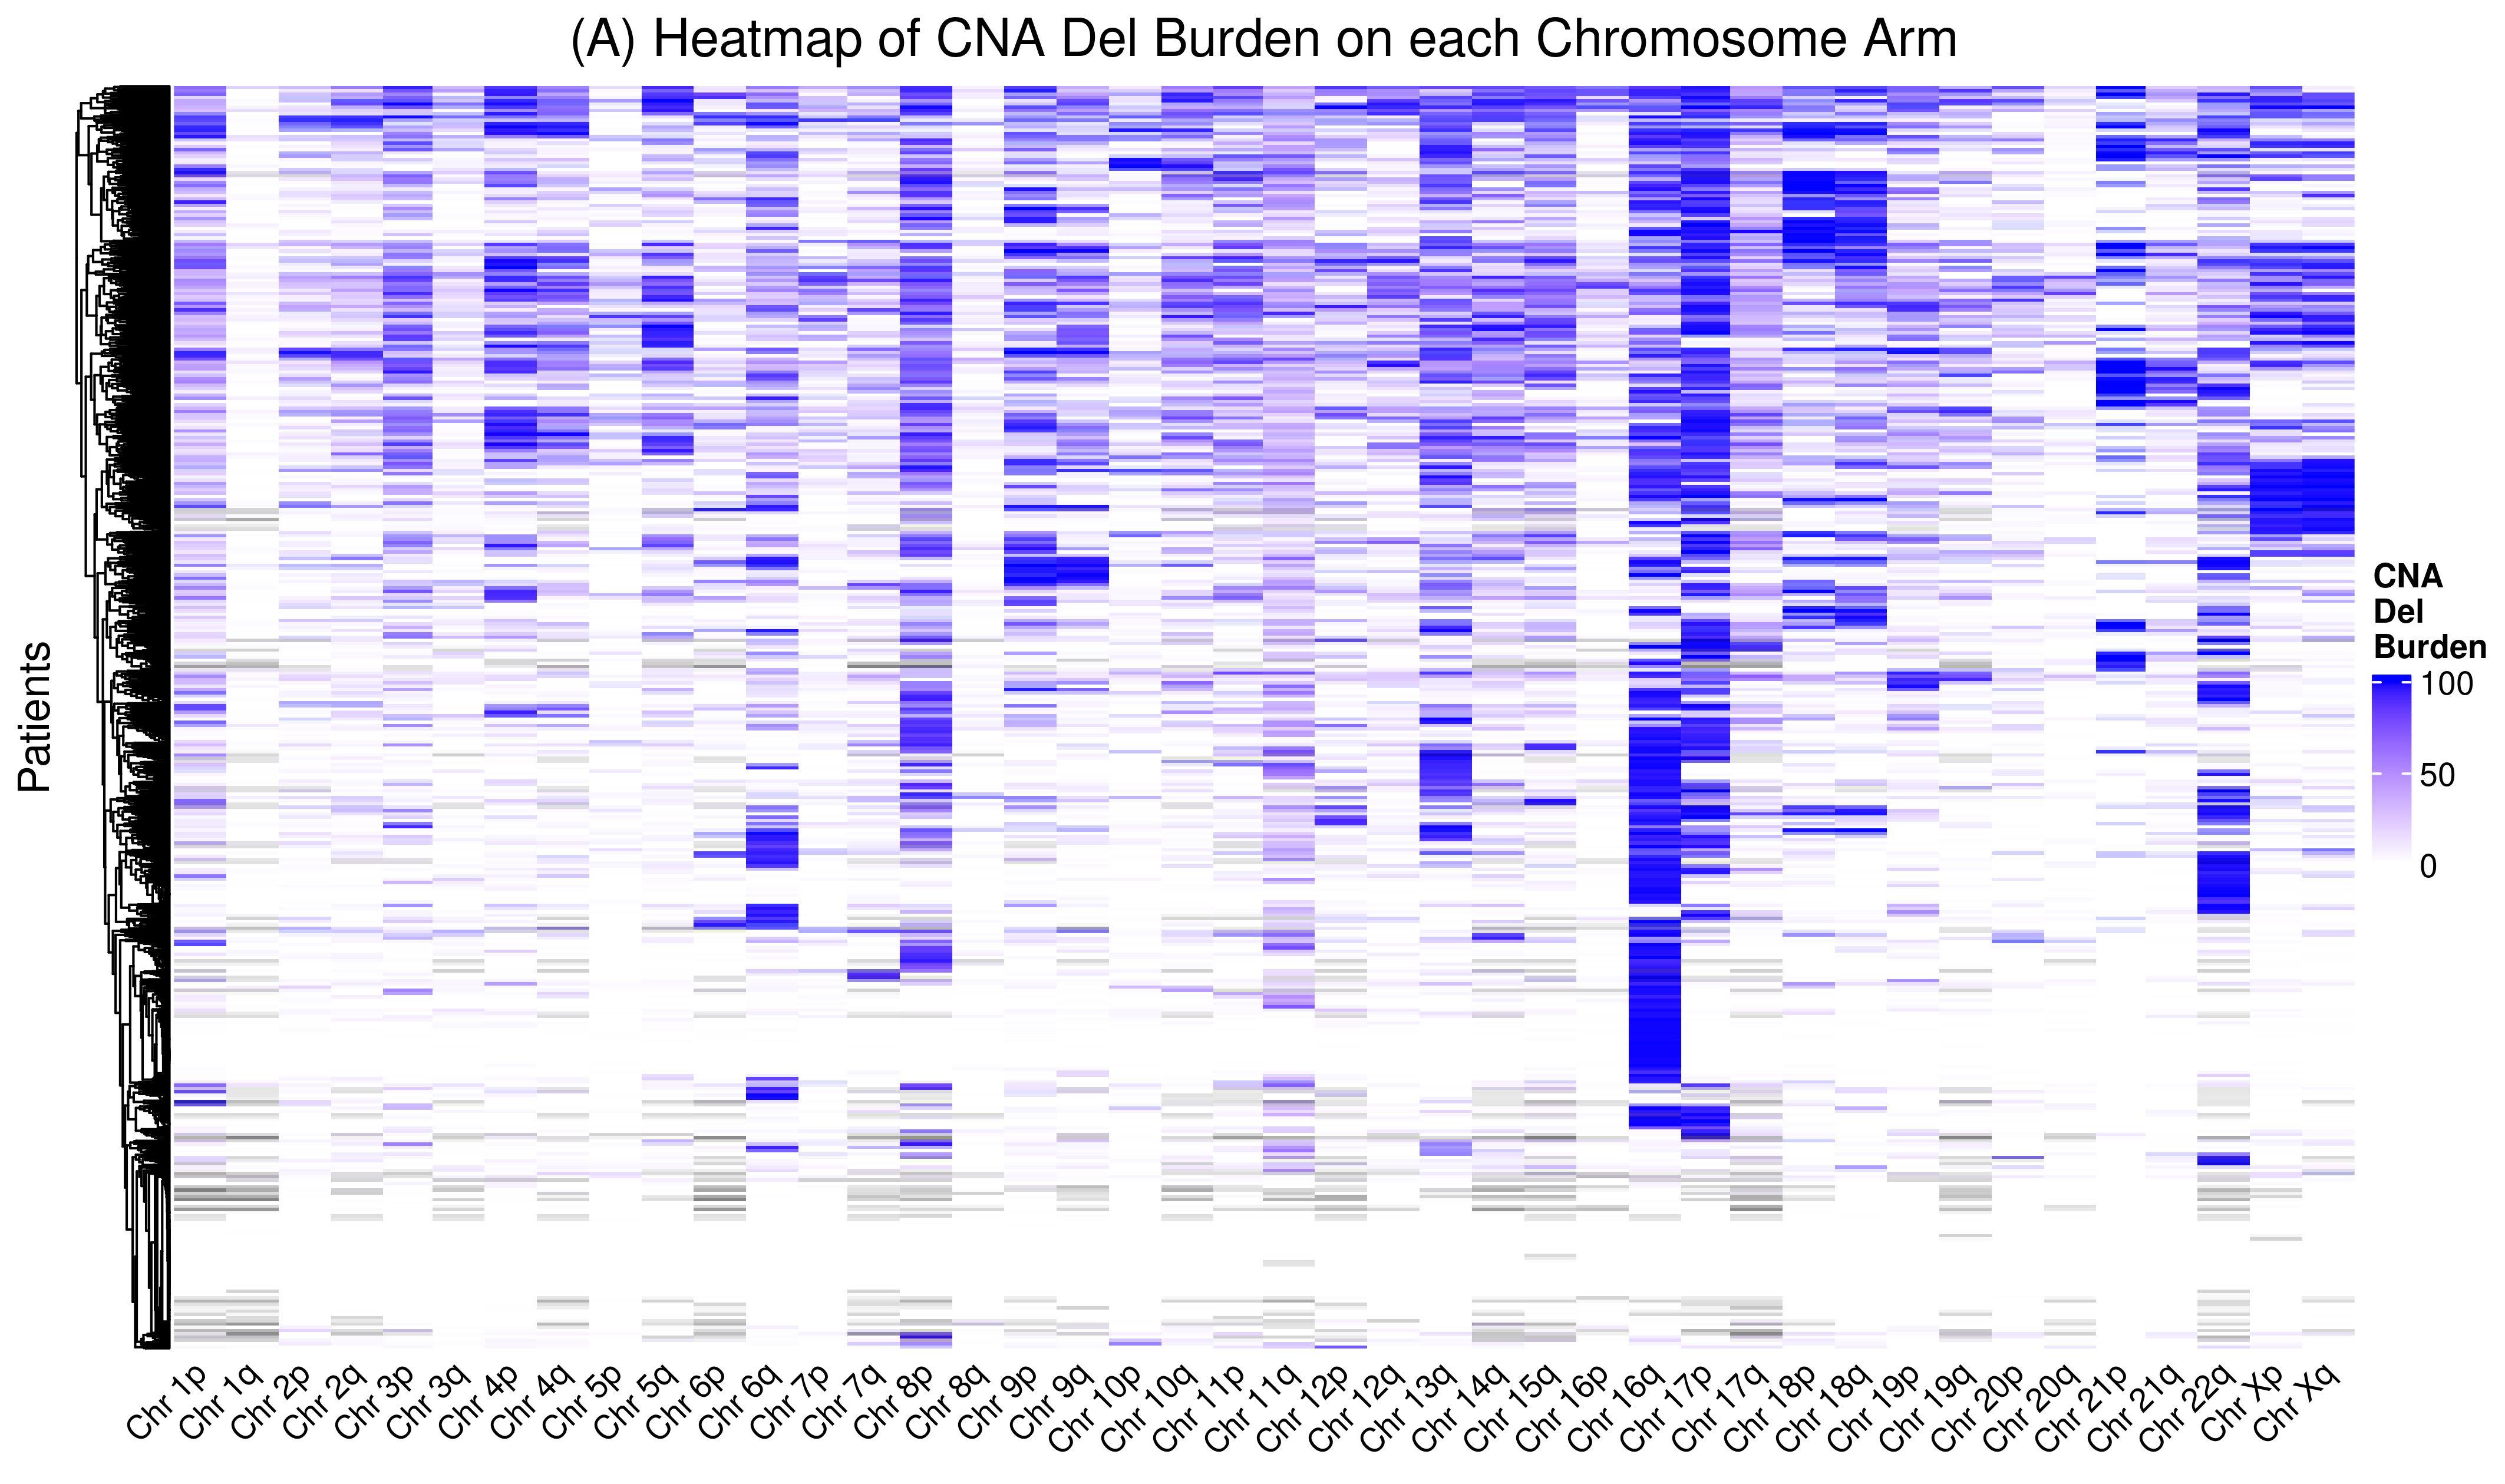
\includegraphics[width = 1.05\textwidth]{../figures/Chapter_2/CNA_Del_Burden_Heatmap_CCA.png}
    
  \vspace{1.5cm}
   
  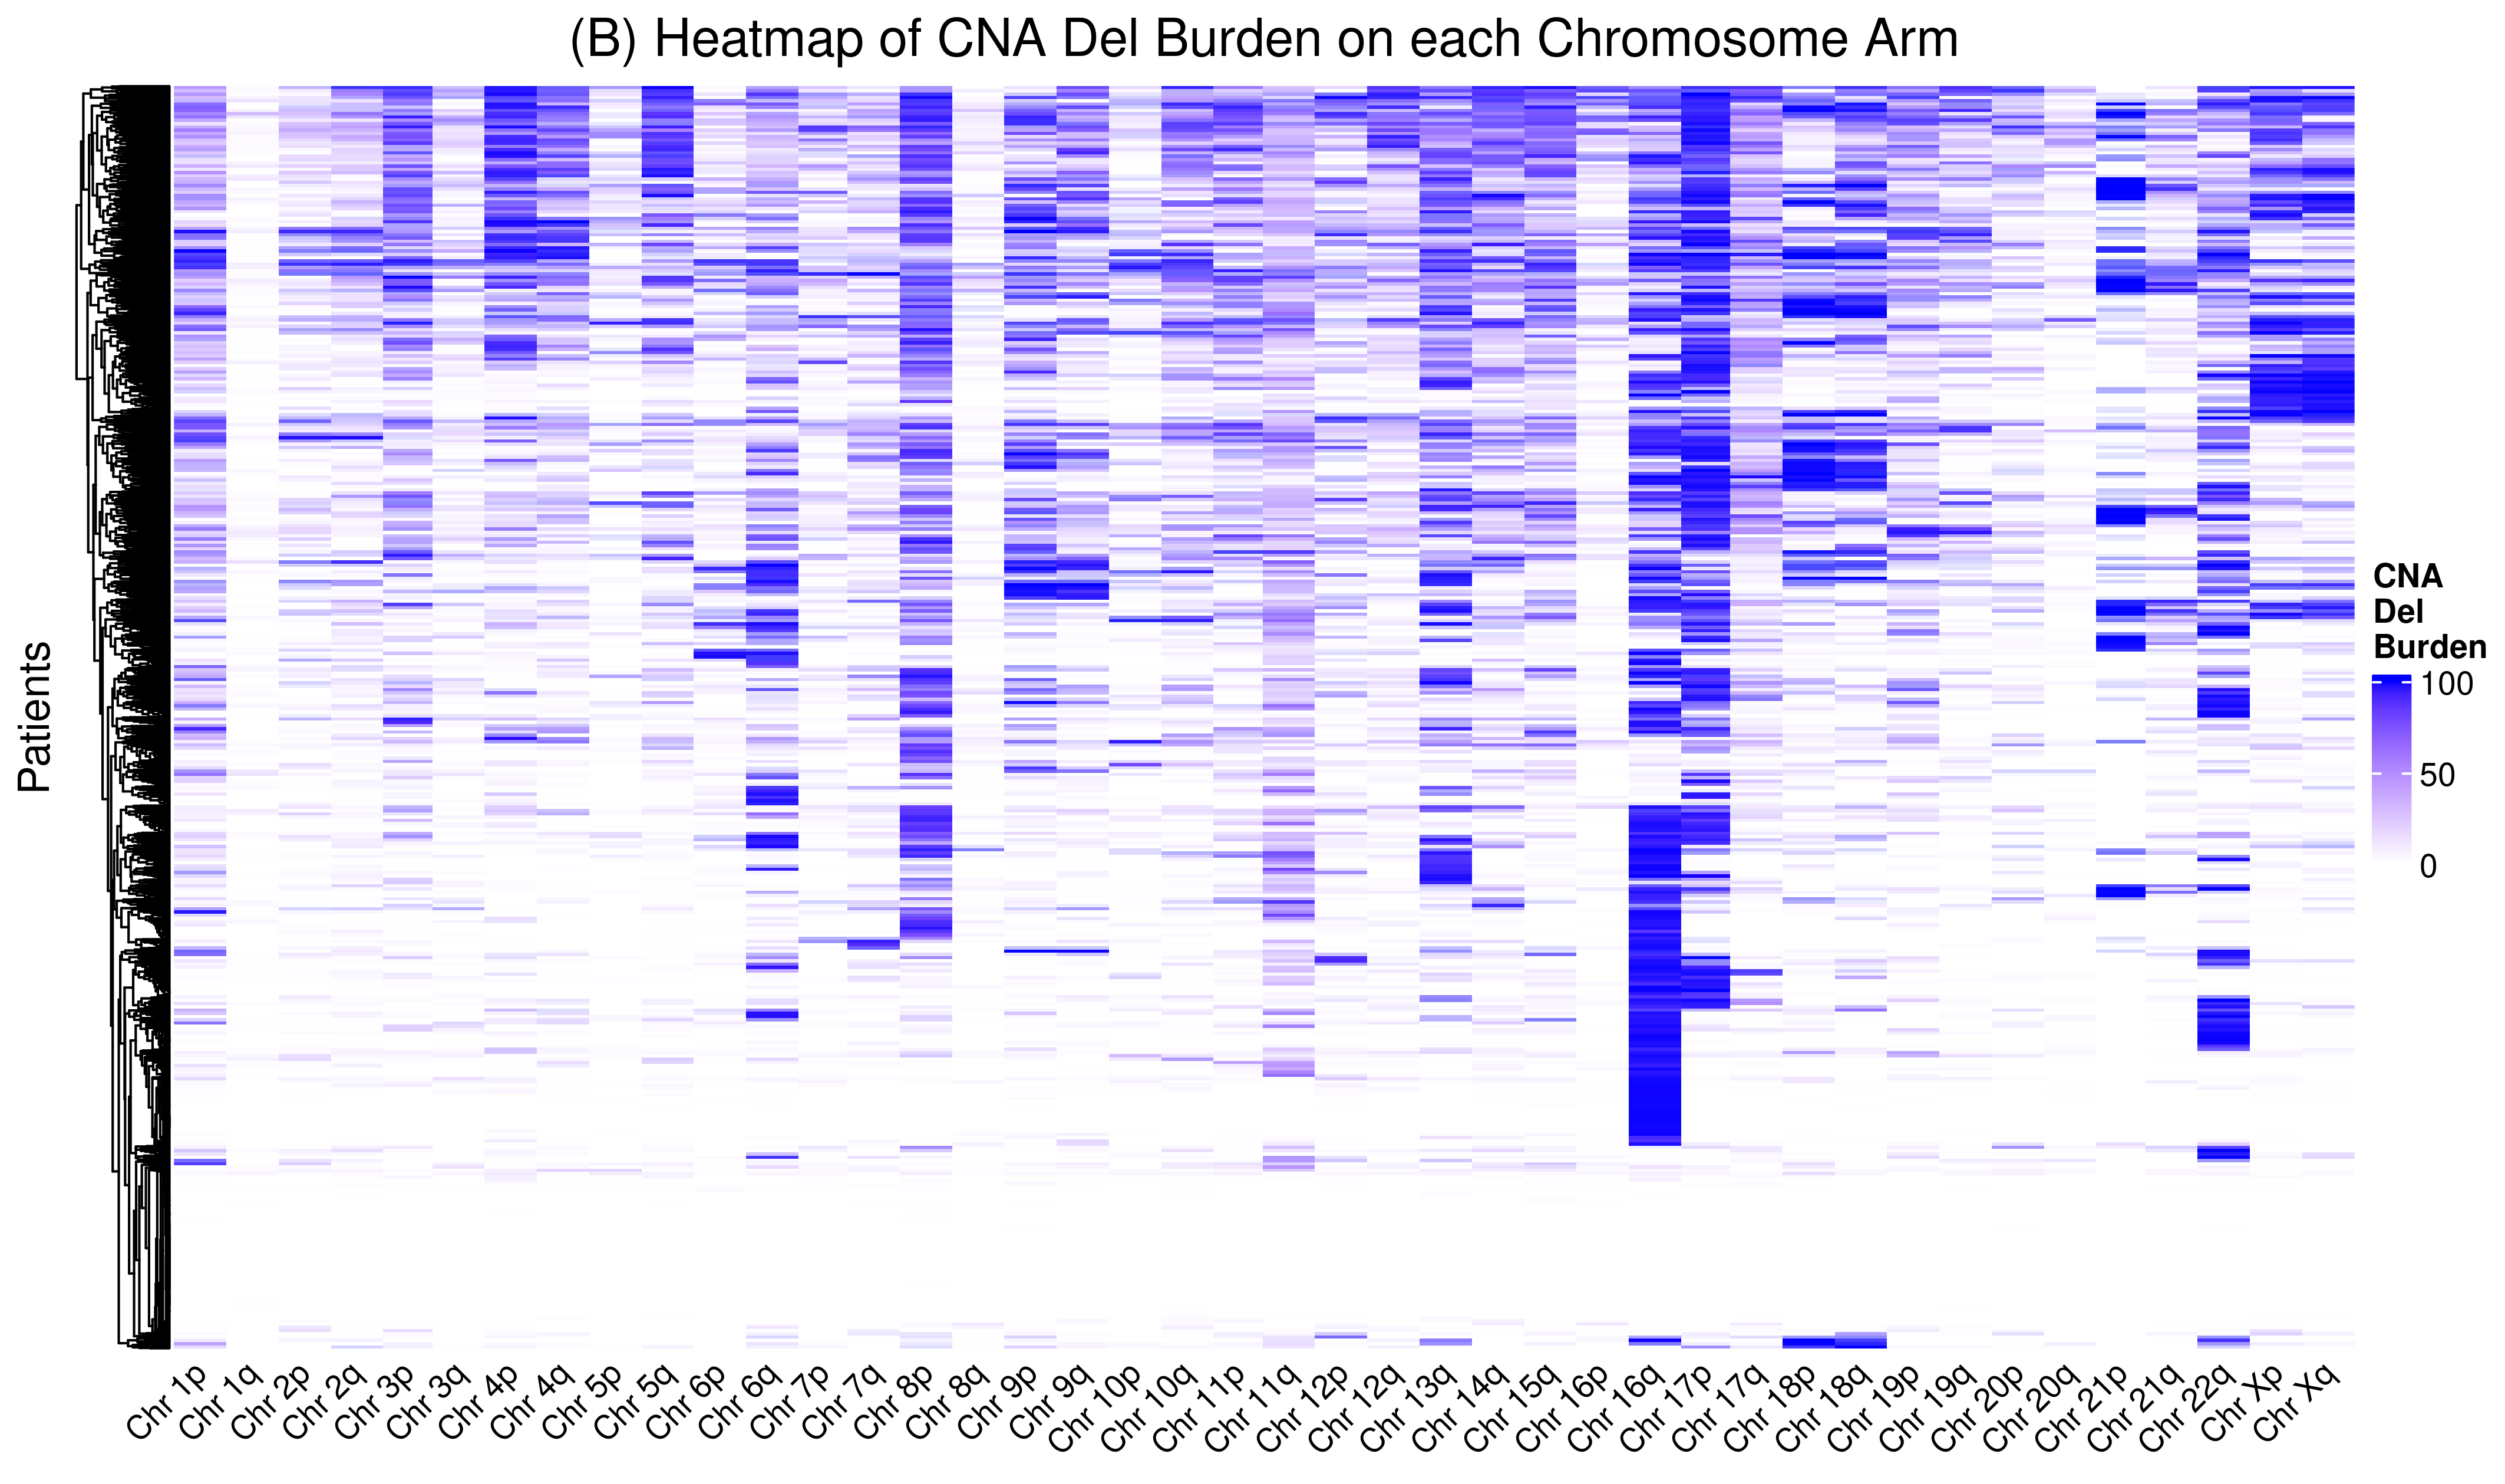
\includegraphics[width = 1.05\textwidth]{../figures/Chapter_2/CNA_Del_Burden_Heatmap_All.png}
  
  \vspace{0.8cm}
  
   \caption[Heatmap of CNA Del Burden across chromosome arms.]{Heatmap of CNA Del Burden across chromosome arms with (A) consideration to complete-case METABRIC patients only (n = 2,091) and (B) consideration to all METABRIC patients including those presenting with some missing data (n = 2,173). Grey indicates missing values.}
  \label{SurvTrees_Burden_HM}
\end{figure}

\begin{table}[!ht]
    \begin{minipage}{.49\linewidth}
      \caption[Chromosomes arms with poor overlap between complete-case patient and all-patient CNA Score metrics.]{Chromosomes arms with poor overlap between complete-case patient and all-patient CNA Score metrics. Metrics are ordered and coloured by percentage overlap.}
      \centering 
\begin{tabular}[t]{l>{}r}
\toprule
CNA Score Metric & \% Overlap\\
\midrule
\% CNA Score Amp 9p & \cellcolor[HTML]{414487}{\textcolor{white}{11.00}}\\
 
CNA Amp Score 9p & \cellcolor[HTML]{443C84}{\textcolor{white}{16.69}}\\
 
\% CNA Score Del 7p & \cellcolor[HTML]{481F70}{\textcolor{white}{42.65}}\\
 
\% CNA Score Amp 18q & \cellcolor[HTML]{481466}{\textcolor{white}{55.59}}\\
 
Difference 18p & \cellcolor[HTML]{450458}{\textcolor{white}{74.15}}\\
 
\% CNA Score Del 8q & \cellcolor[HTML]{450457}{\textcolor{white}{75.14}}\\
 
\% CNA Score Amp 22q & \cellcolor[HTML]{440256}{\textcolor{white}{76.71}}\\
 
Difference Xq & \cellcolor[HTML]{440155}{\textcolor{white}{77.85}}\\
 
Difference 18q & \cellcolor[HTML]{440155}{\textcolor{white}{78.80}}\\
 
Difference 19p & \cellcolor[HTML]{440154}{\textcolor{white}{79.10}}\\
\bottomrule
\end{tabular} \label{table:CNAScoreT2}
    \end{minipage}%
    \hspace{0.3cm}
    \begin{minipage}{.49\linewidth}
      \centering
      \caption[Chromosomes arms with poor overlap between complete-case patient and all-patient CNA Burden metrics.]{Chromosomes arms with poor overlap between complete-case patient and all-patient CNA Burden metrics. Metrics are ordered and coloured by percentage overlap.}
\begin{tabular}[t]{l>{}r}
\toprule
CNA Burden Metric & \% Overlap\\
\midrule
\% CNA Burden Amp 9p & \cellcolor[HTML]{414487}{\textcolor{white}{10.84}}\\
 
CNA Amp Burden 9p & \cellcolor[HTML]{443B84}{\textcolor{white}{16.83}}\\
 
\% CNA Burden Del 7p & \cellcolor[HTML]{481C6E}{\textcolor{white}{45.26}}\\
 
\% CNA Burden Amp 18q & \cellcolor[HTML]{460B5E}{\textcolor{white}{65.25}}\\
 
CNA Amp Burden Xq & \cellcolor[HTML]{46075B}{\textcolor{white}{67.35}}\\
 
Difference 19p & \cellcolor[HTML]{46065A}{\textcolor{white}{70.39}}\\
 
\% CNA Burden Amp 22q & \cellcolor[HTML]{450457}{\textcolor{white}{72.01}}\\
 
Difference 18p & \cellcolor[HTML]{450357}{\textcolor{white}{76.29}}\\
 
Difference Xq & \cellcolor[HTML]{440154}{\textcolor{white}{77.29}}\\
 
Difference 18q & \cellcolor[HTML]{440154}{\textcolor{white}{79.68}}\\
\bottomrule
\end{tabular} \label{table:CNABurdenT2}
    \end{minipage}
\end{table}

\vfill
\begin{figure}[H]
\vspace{0.1cm}
\begin{minipage}{.49\textwidth}
    \subfloat[]{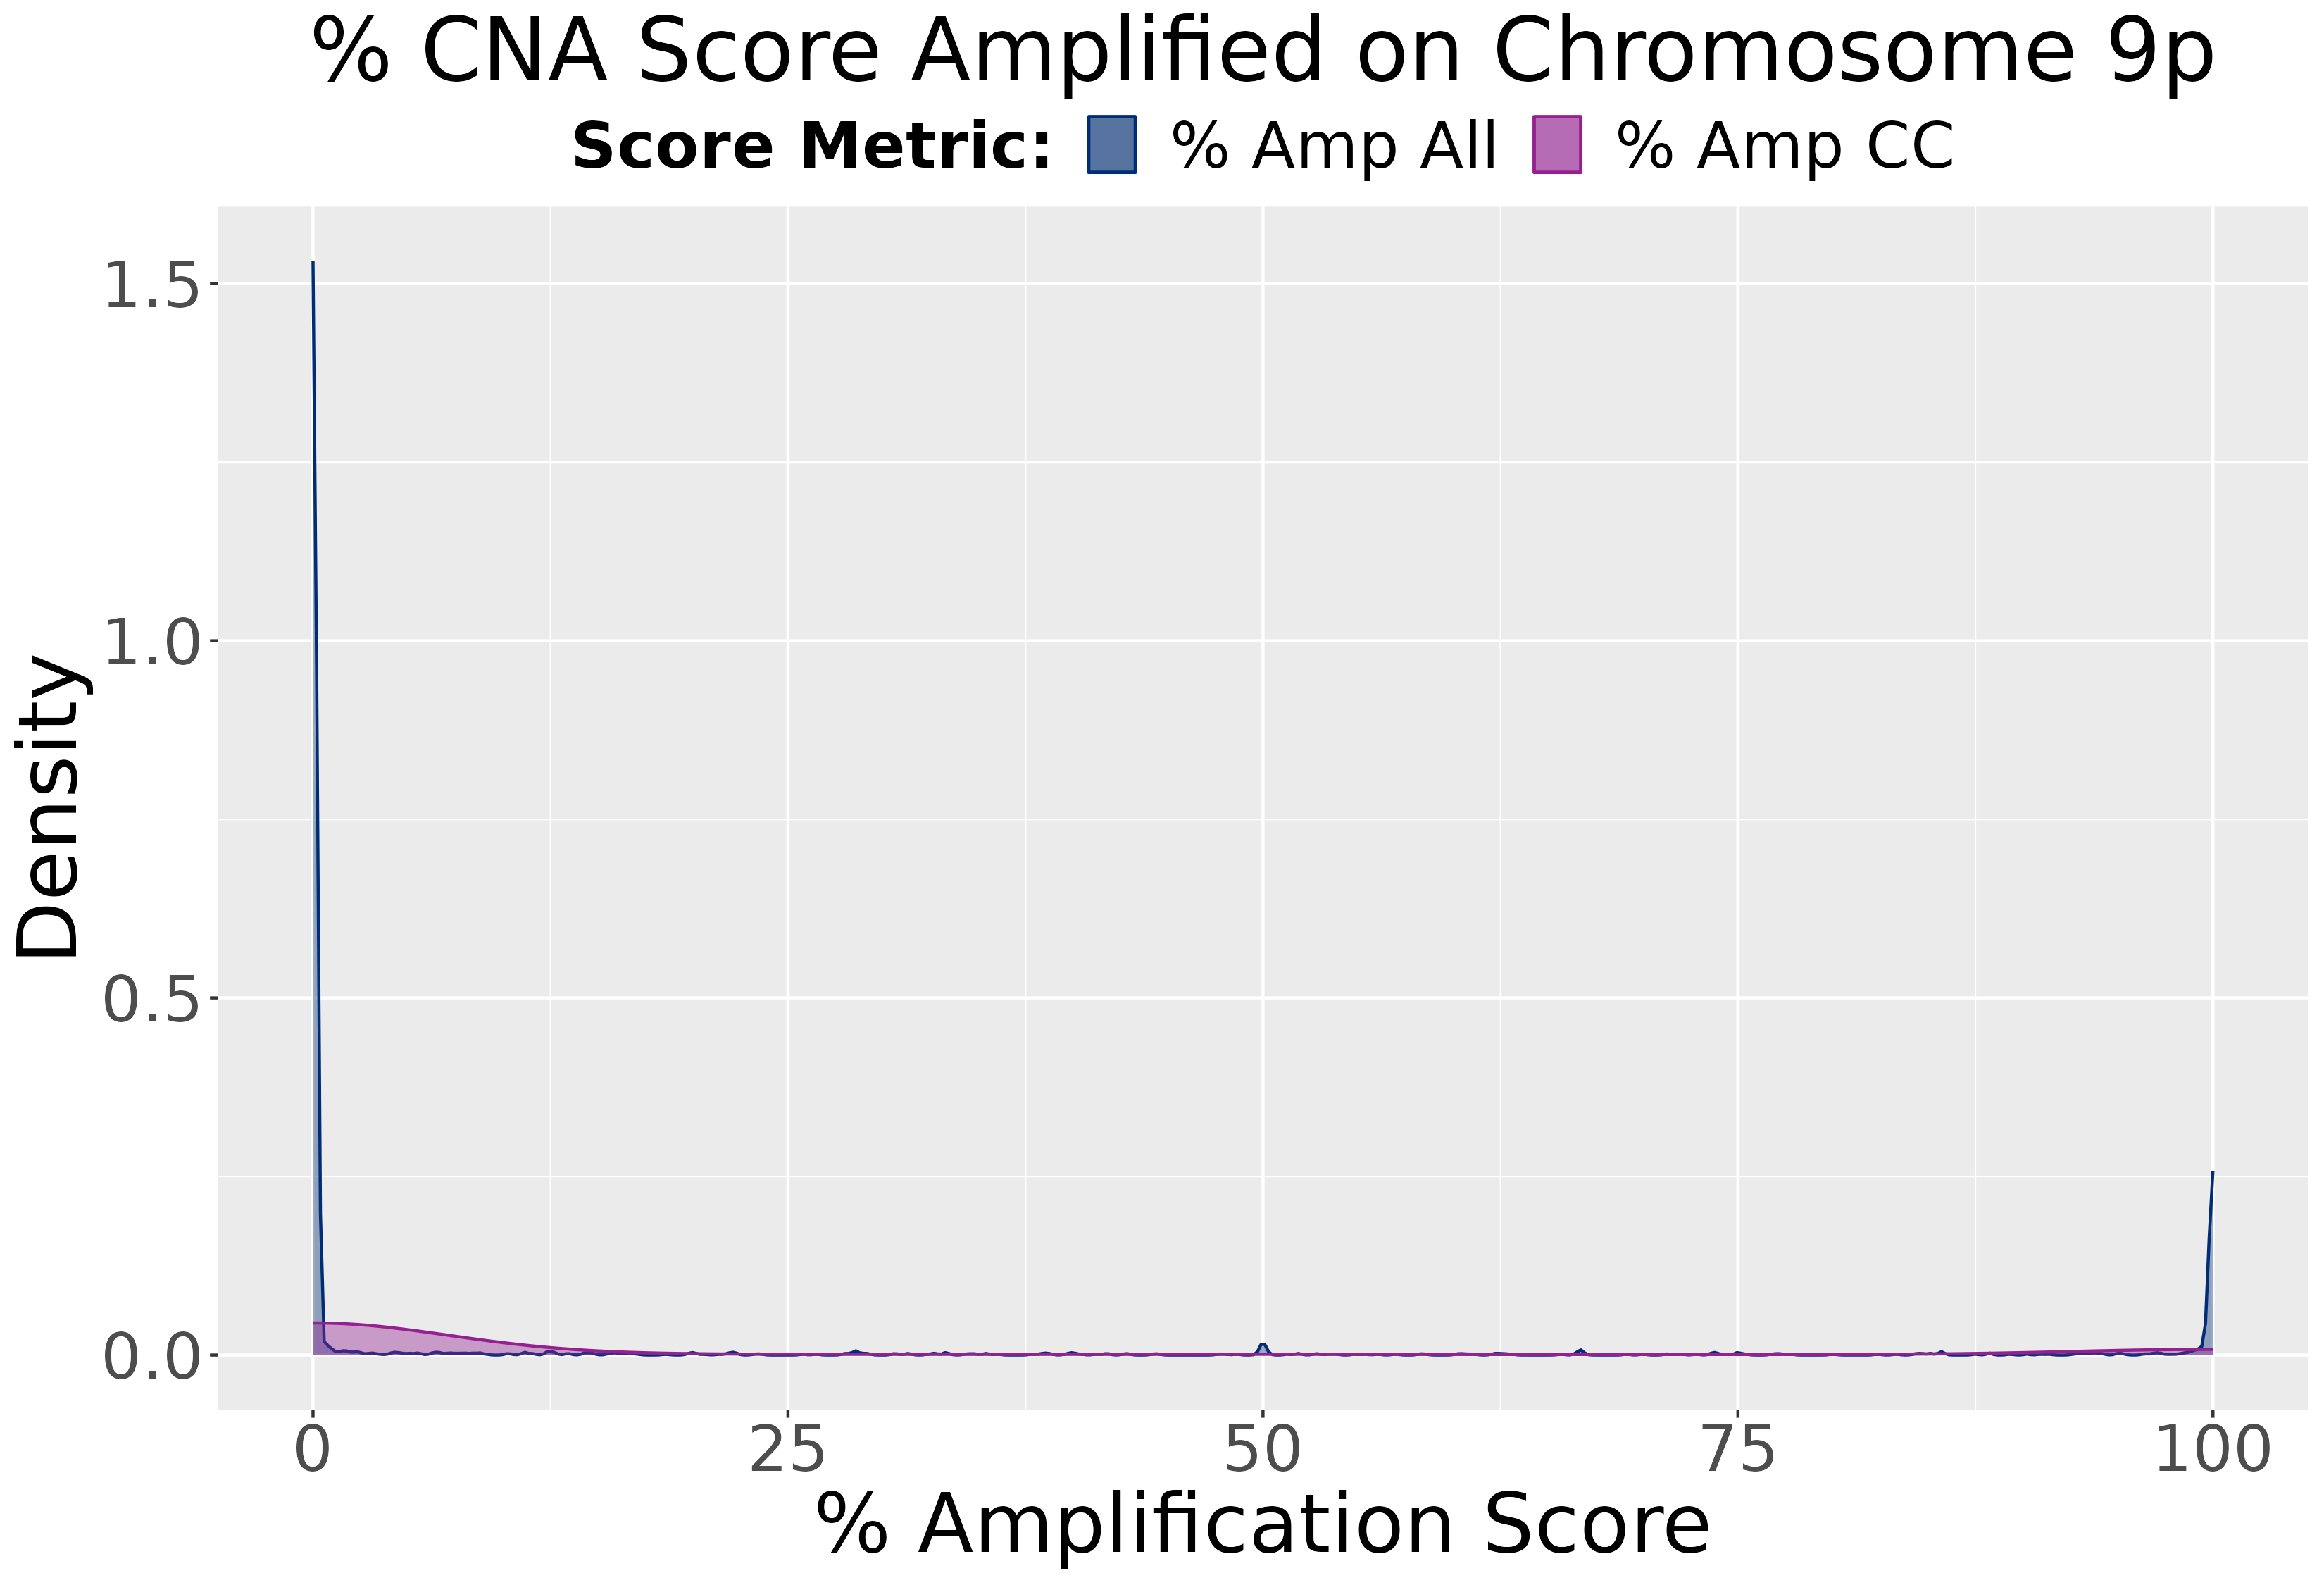
\includegraphics[width=\textwidth]{../figures/Chapter_2/CNA_Score_9p.png}}
\end{minipage}
\hfill   
\begin{minipage}{.49\textwidth}
    \subfloat[]{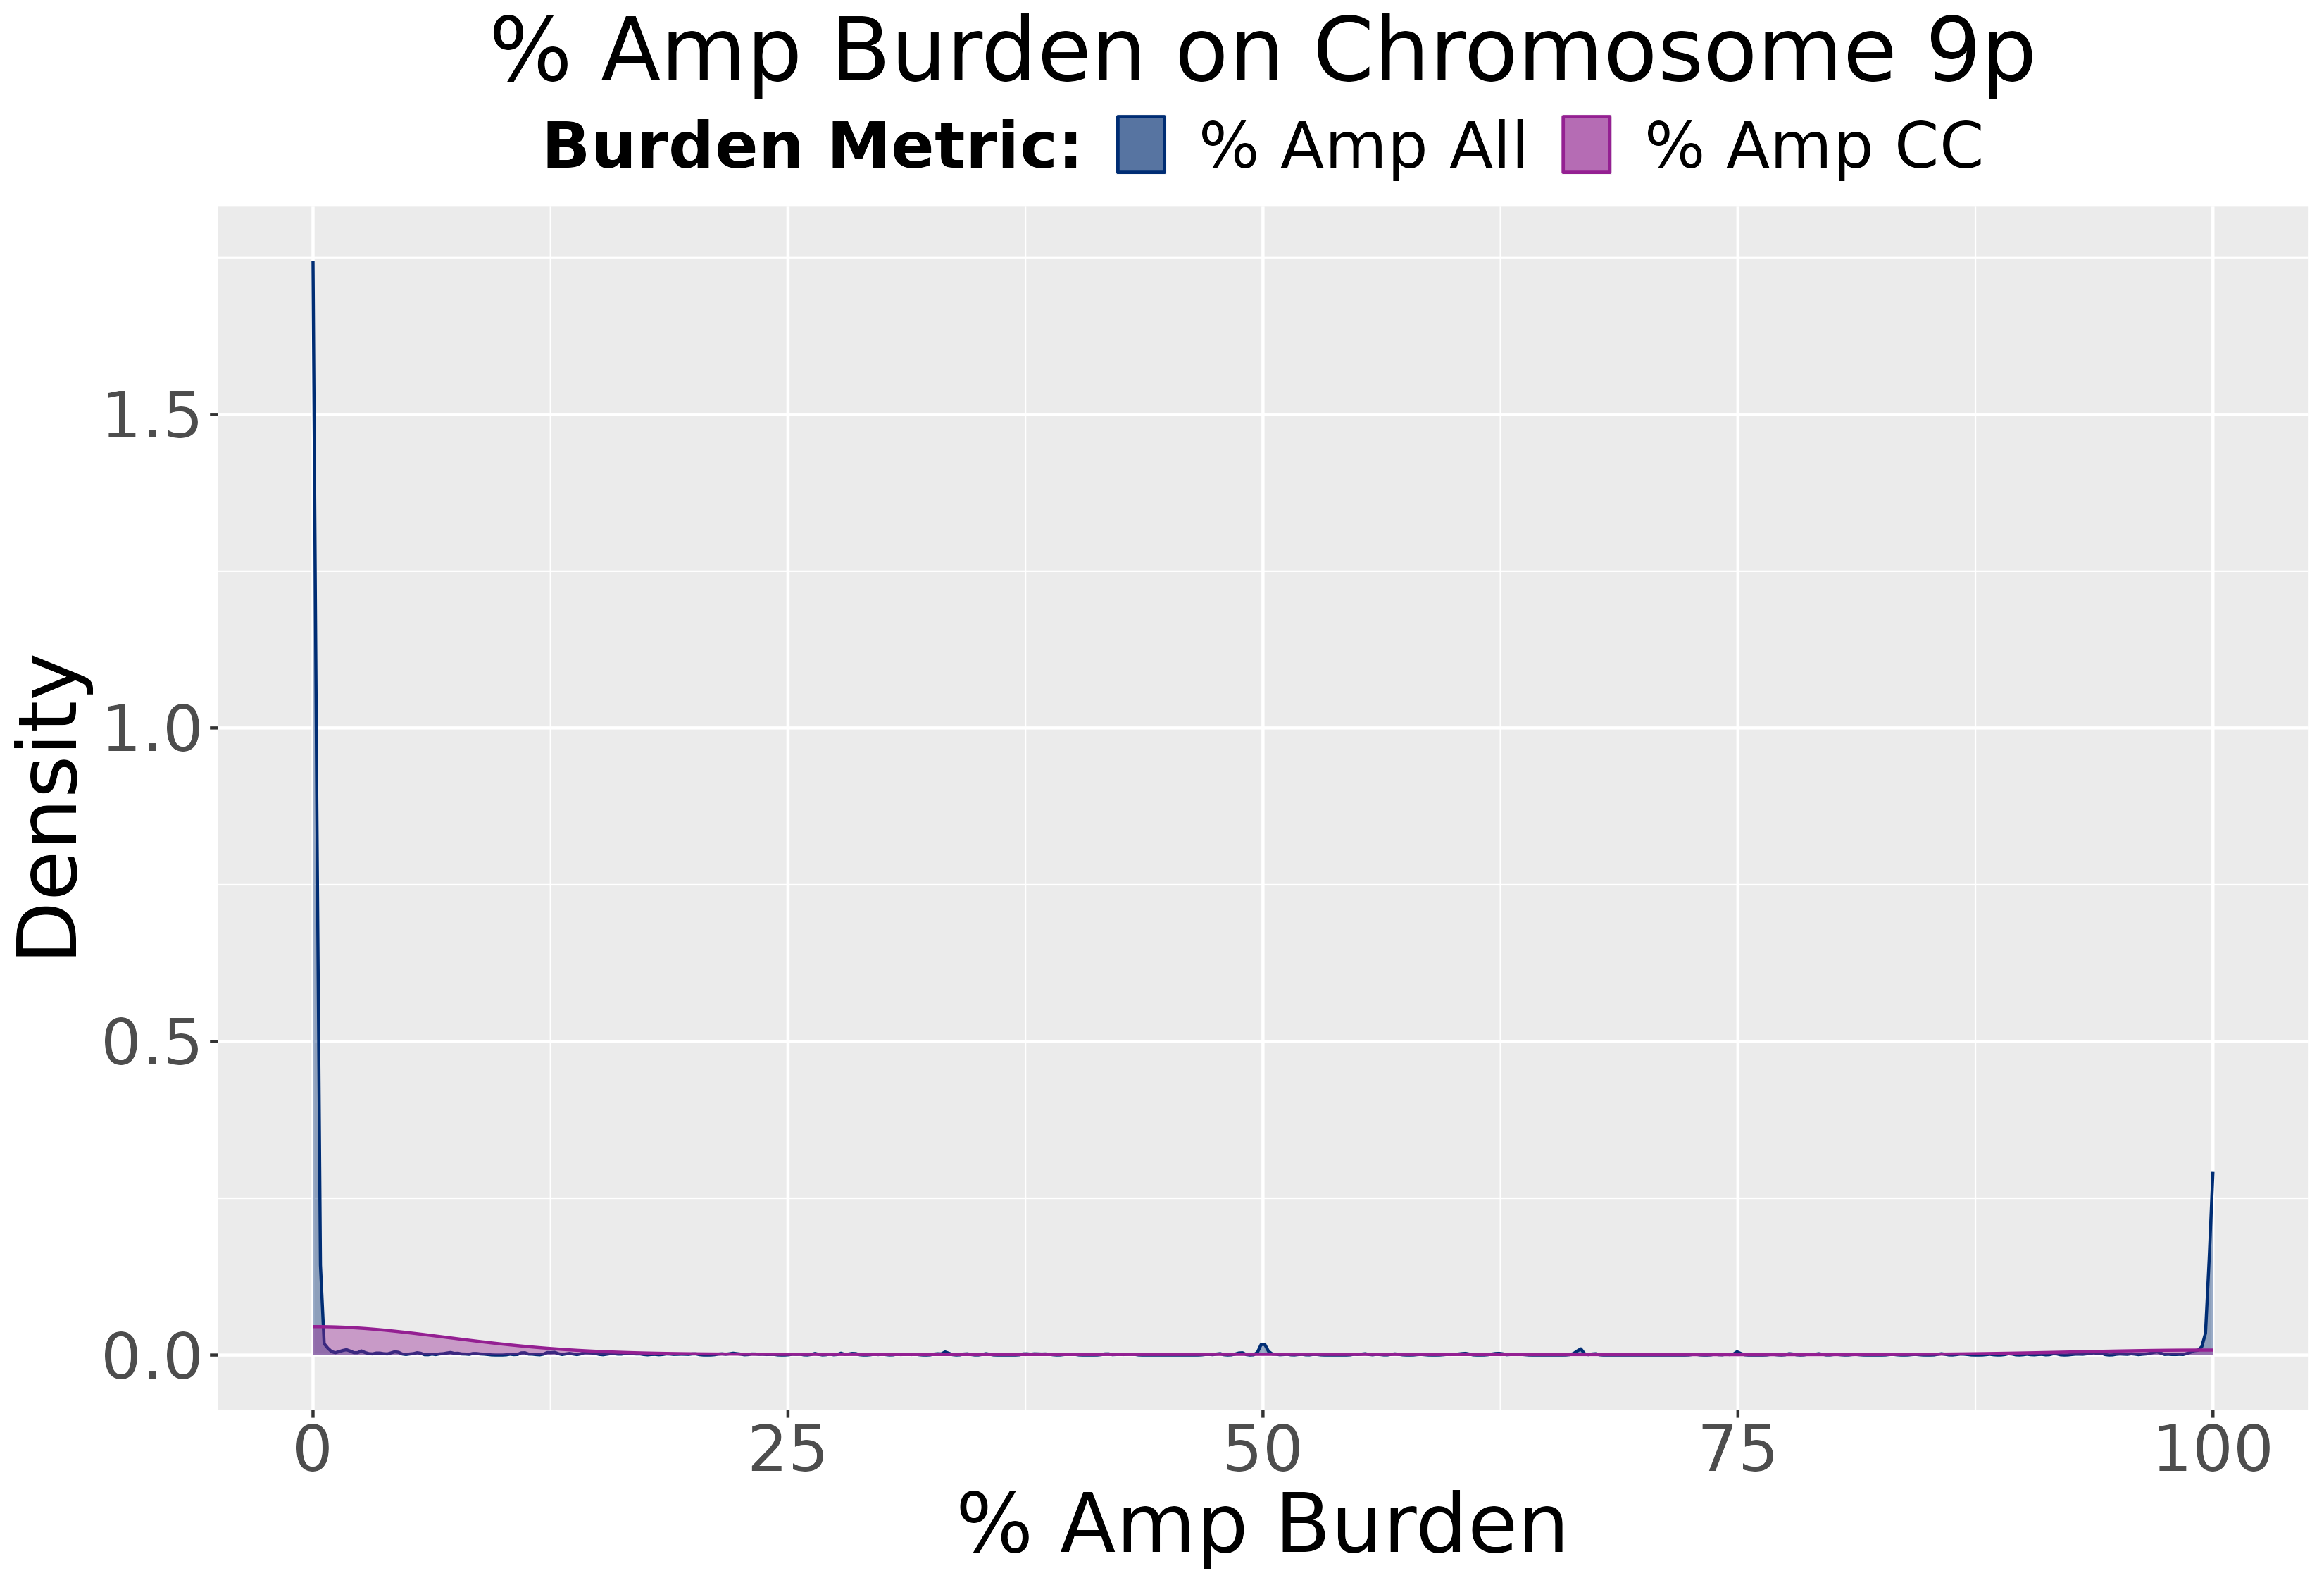
\includegraphics[width=\textwidth]{../figures/Chapter_2/CNA_Burden_9p.png}}
\end{minipage}
\hfill
\begin{minipage}{.49\textwidth}
    \subfloat[]{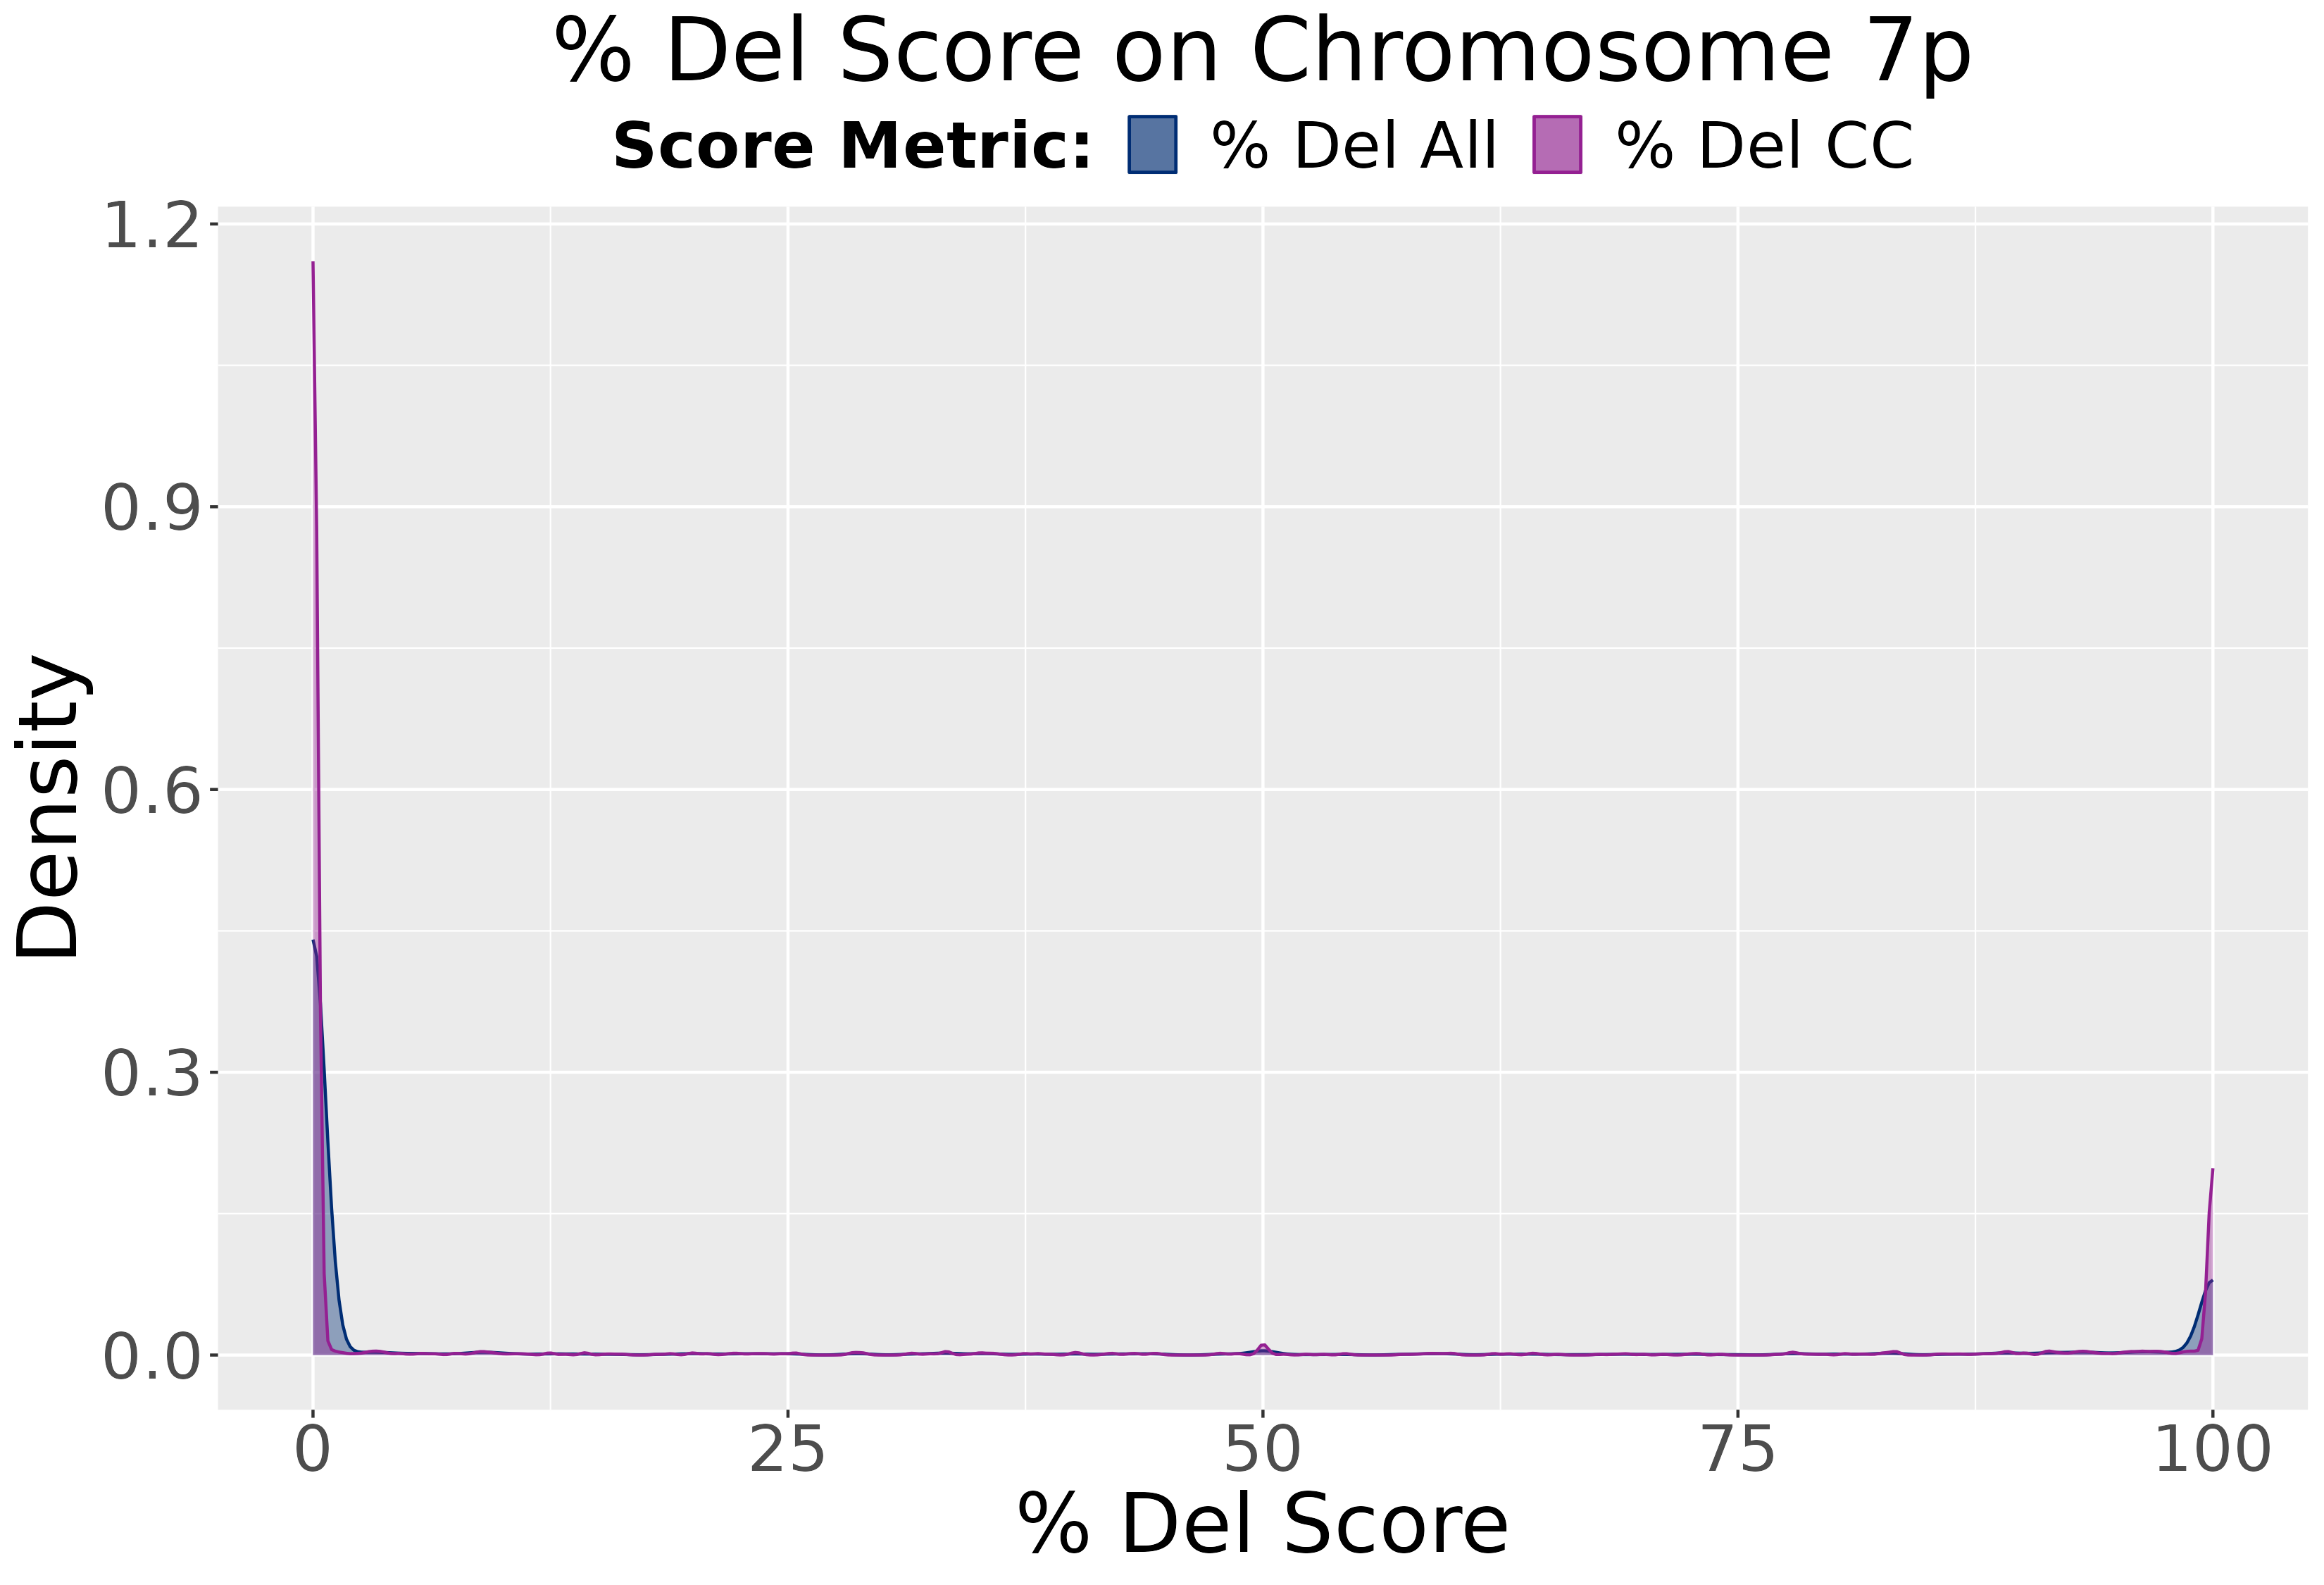
\includegraphics[width=\textwidth]{../figures/Chapter_2/CNA_Score_7p.png}}
\end{minipage}
\hfill    
\begin{minipage}{.49\textwidth}
    \subfloat[]{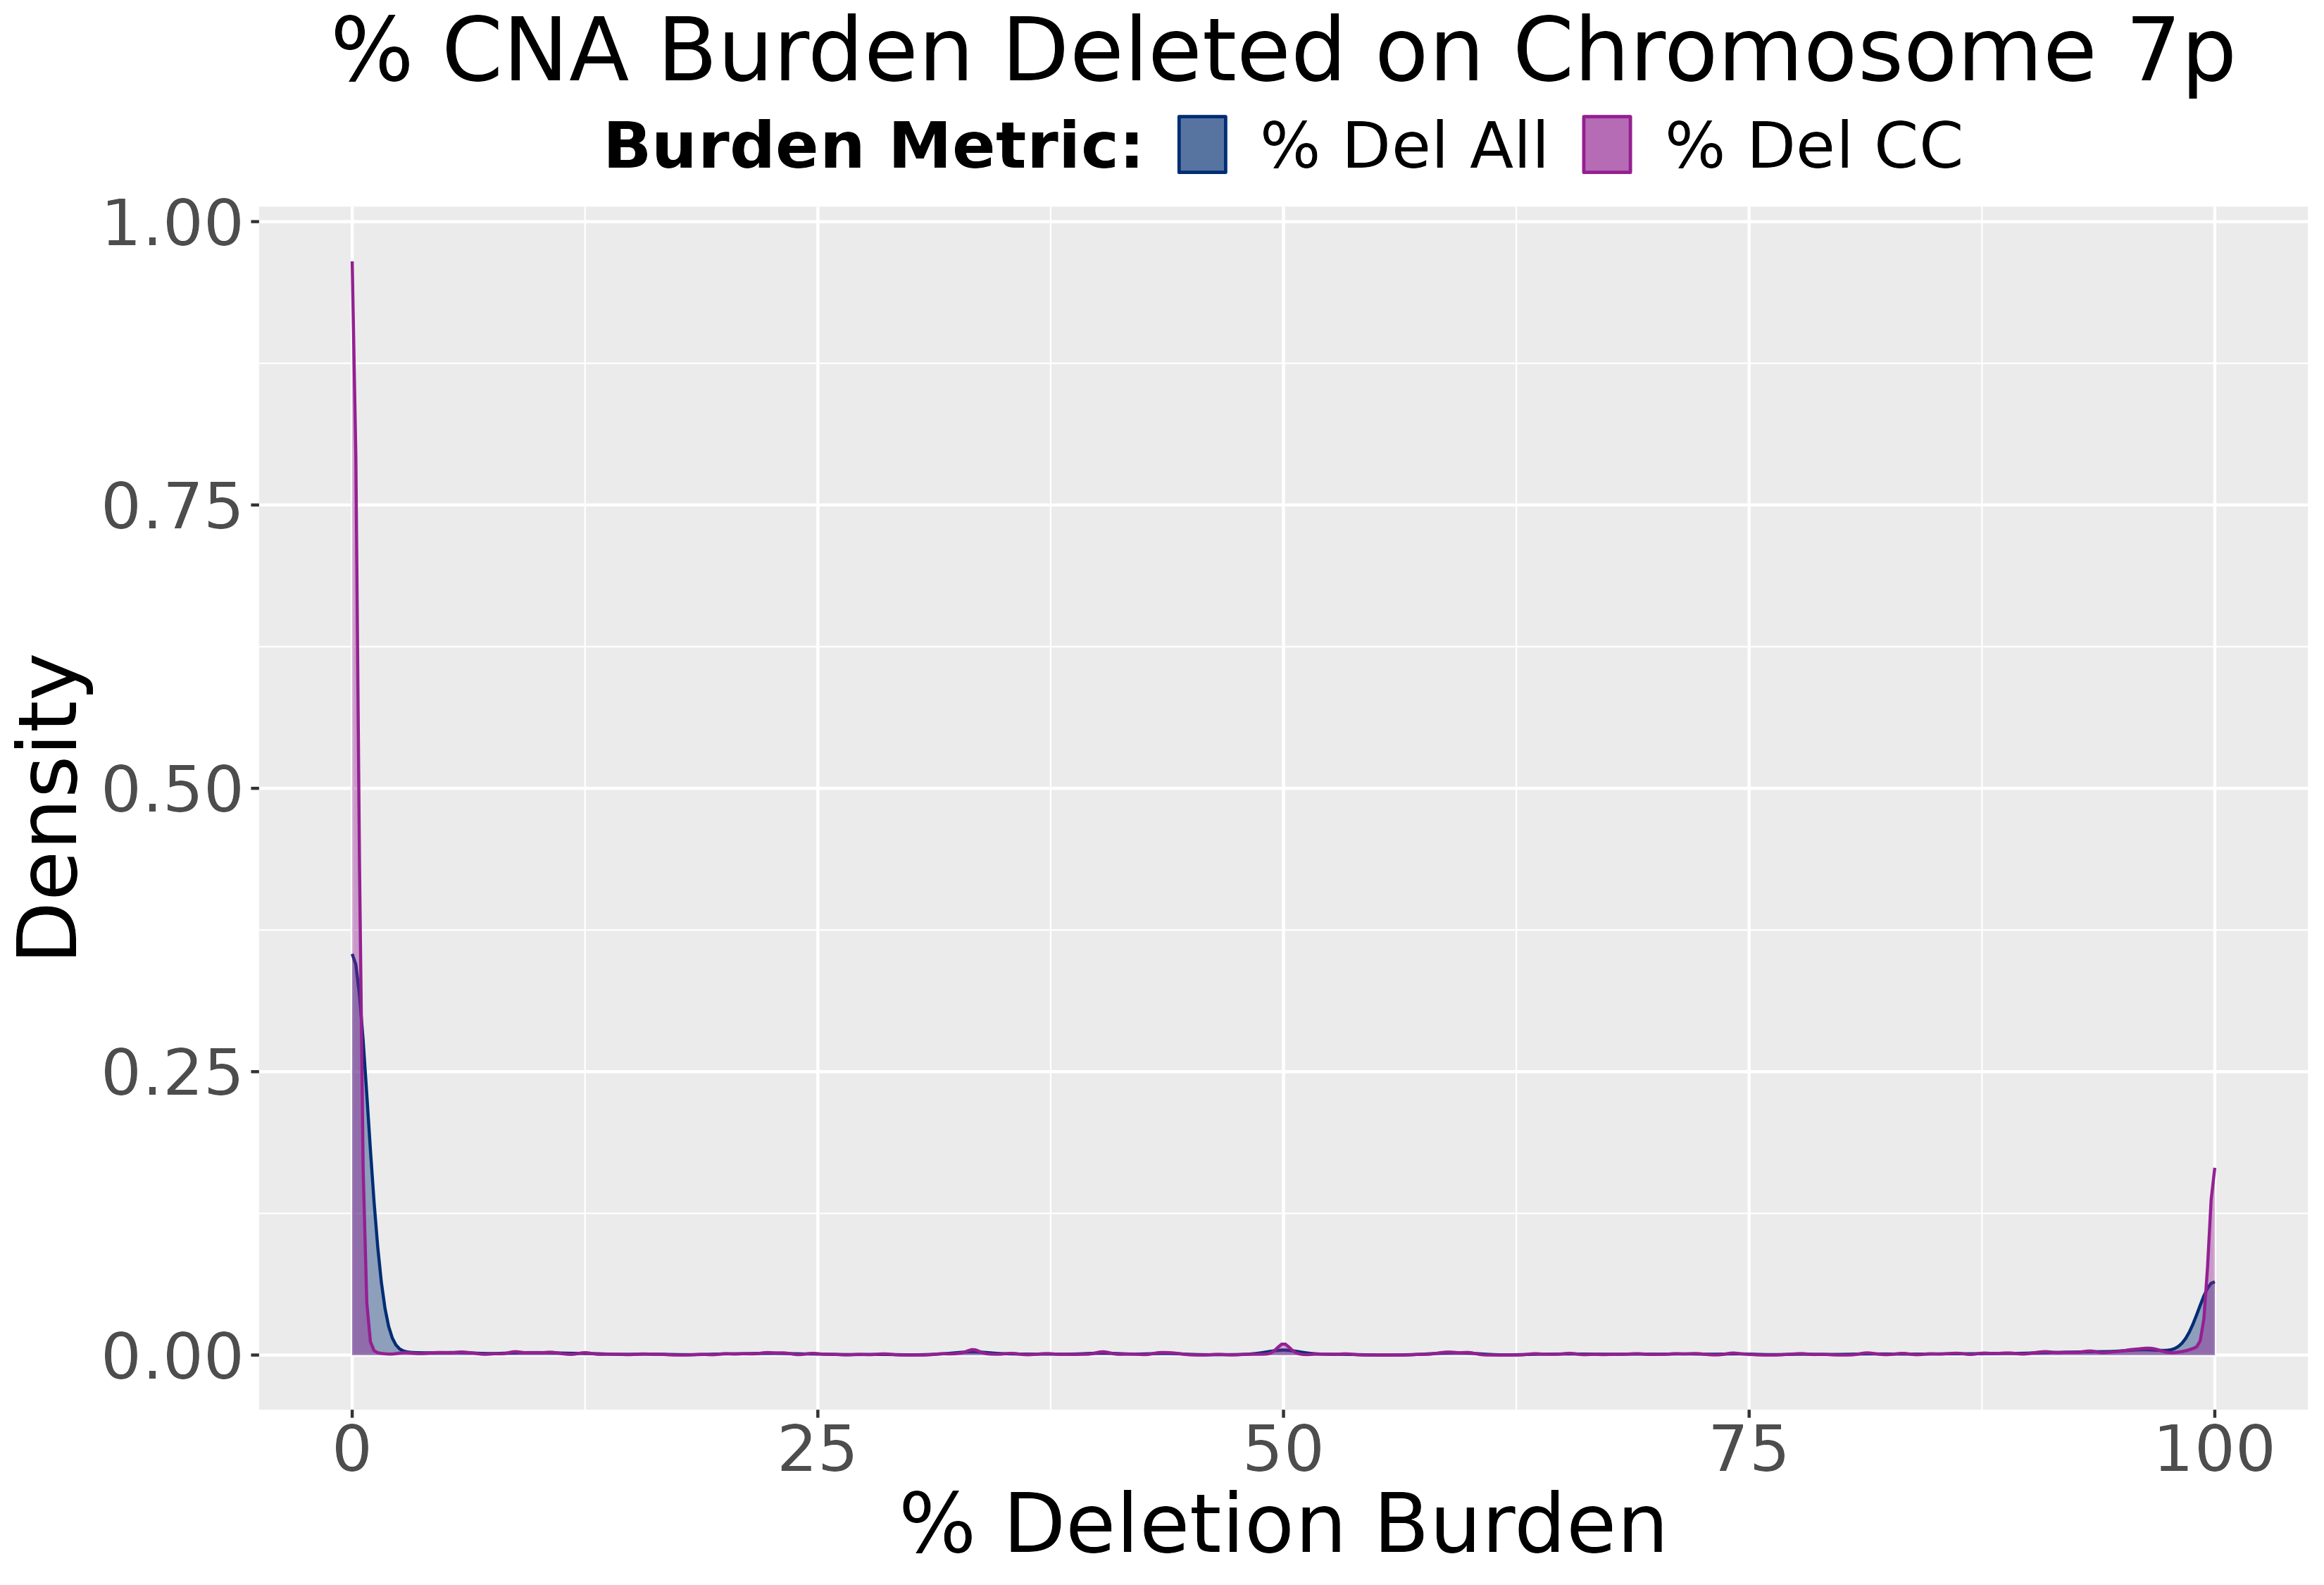
\includegraphics[width=\textwidth]{../figures/Chapter_2/CNA_Burden_7p.png}}
\end{minipage}
    \caption[Density plots for selected chromosome arm CNA metrics.]{Density plots for selected chromosome arm CNA metrics. (A) Percentage CNA Score Amp on chromosome 9p, (B) Percentage CNA Burden Amp on chromosome 9p, (C) Percentage CNA Score Del on chromosome 7p and (D) Percentage CNA Burden Del on chromosome 7p. Each plot contains density plots for both the complete-case metric and the metric calculated using all available data.}\label{fig:Plot-PerArm-DensityPlots}
\end{figure} 
\vfill 

\begin{table}[!ht]
\center
\caption[Summary statistics of the CNA Score metrics on chromosome 1q where all available data are used.]{Summary statistics of the CNA Score metrics on chromosome 1q  where all available data are used.}
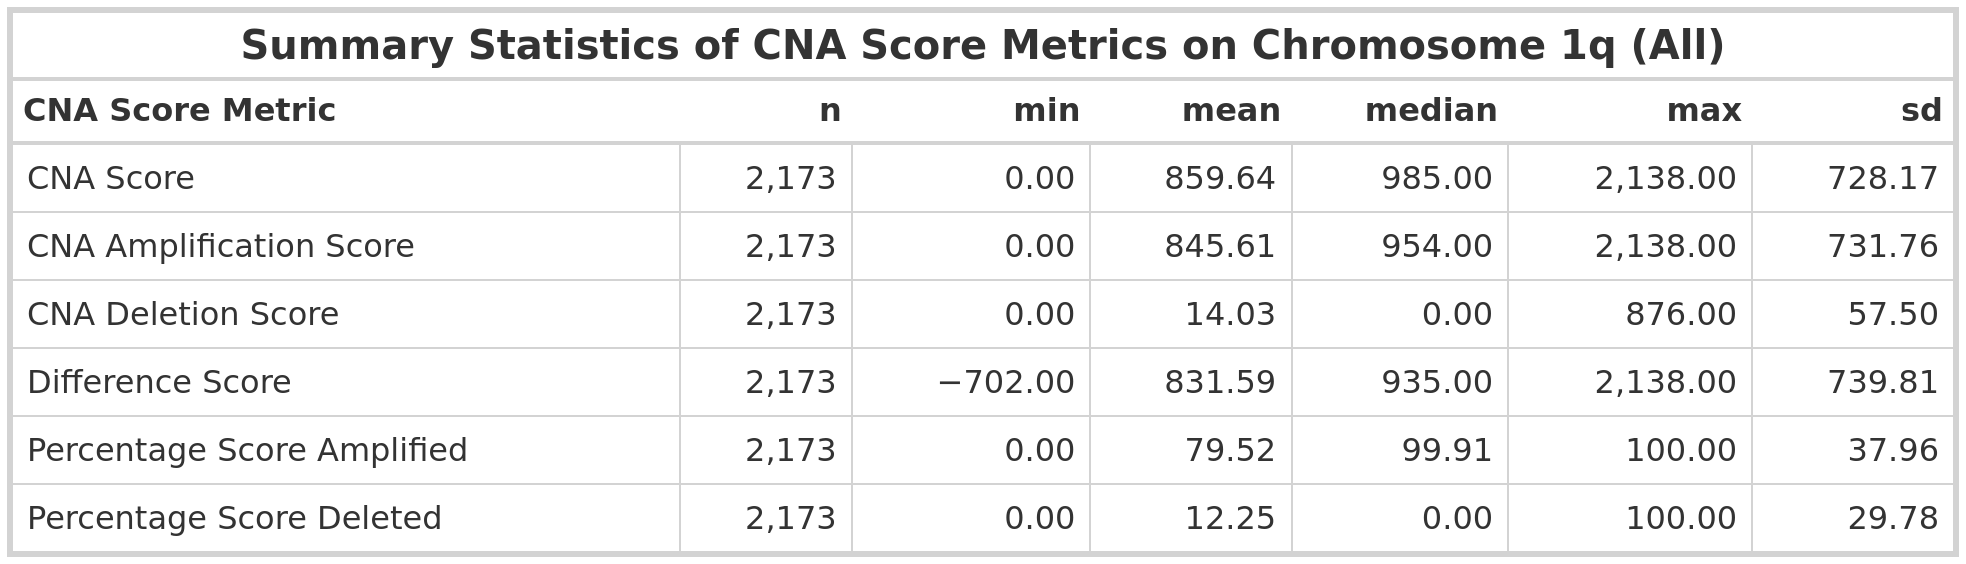
\includegraphics[width = 0.98\textwidth]{../tables/Chapter_2/CNA_Score_Metric_All_Chr1q_Summary.png}
\label{tab:Score_All_Chr1q}
\end{table}

\begin{table}[!ht]
\center
\caption[Summary statistics of the CNA Score metrics on chromosome 1q where only complete cases are used.]{Summary statistics of the CNA Score metrics on chromosome 1q where only complete cases are used.}
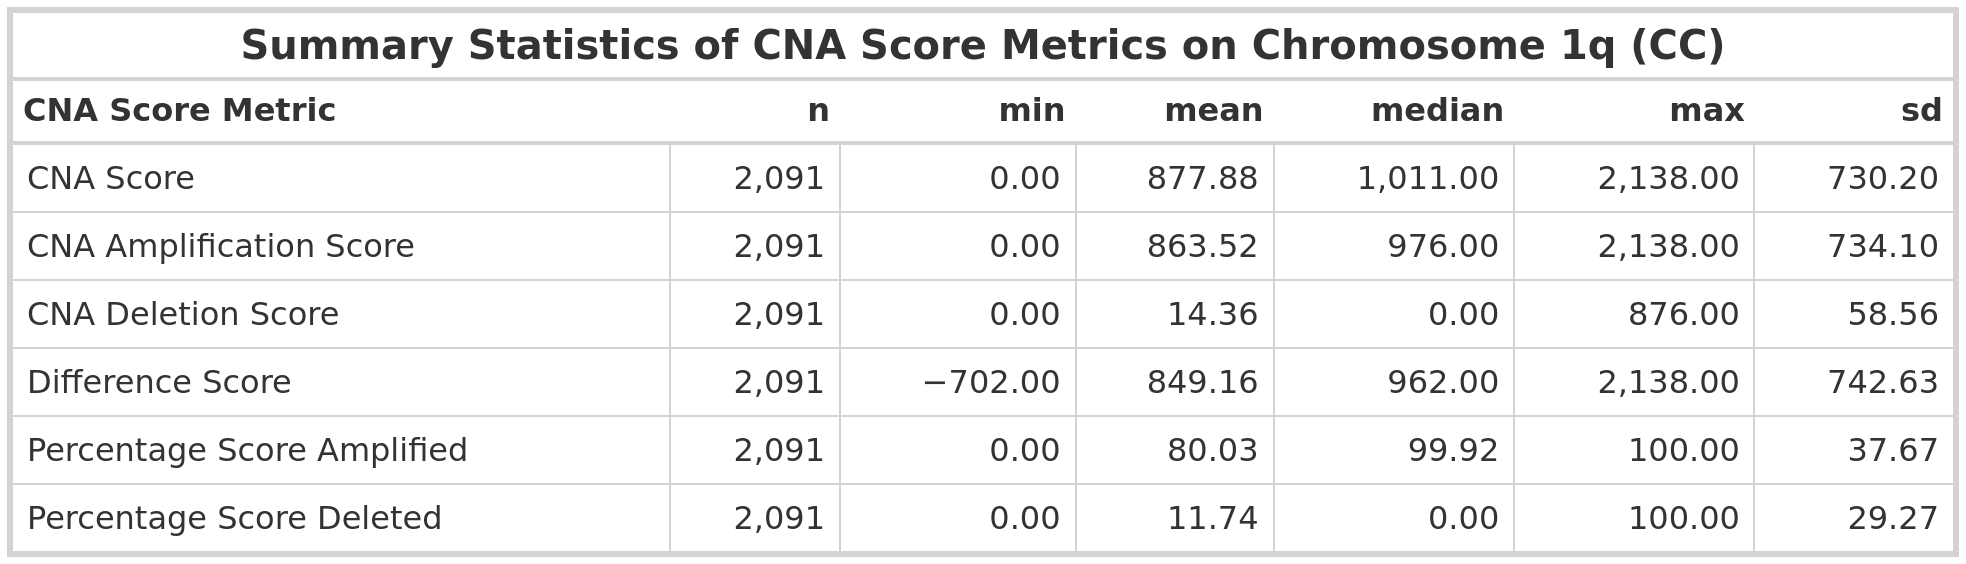
\includegraphics[width = 0.98\textwidth]{../tables/Chapter_2/CNA_Score_Metric_CCA_Chr1q_Summary.png}
\label{tab:Score_CCA_Chr1q}
\end{table}

\begin{table}[!ht]
\center
\caption[Summary statistics of the CNA Burden metrics on chromosome 1q where all available data are used.]{Summary statistics of the CNA Burden metrics on chromosome 1q where all available data are used.}
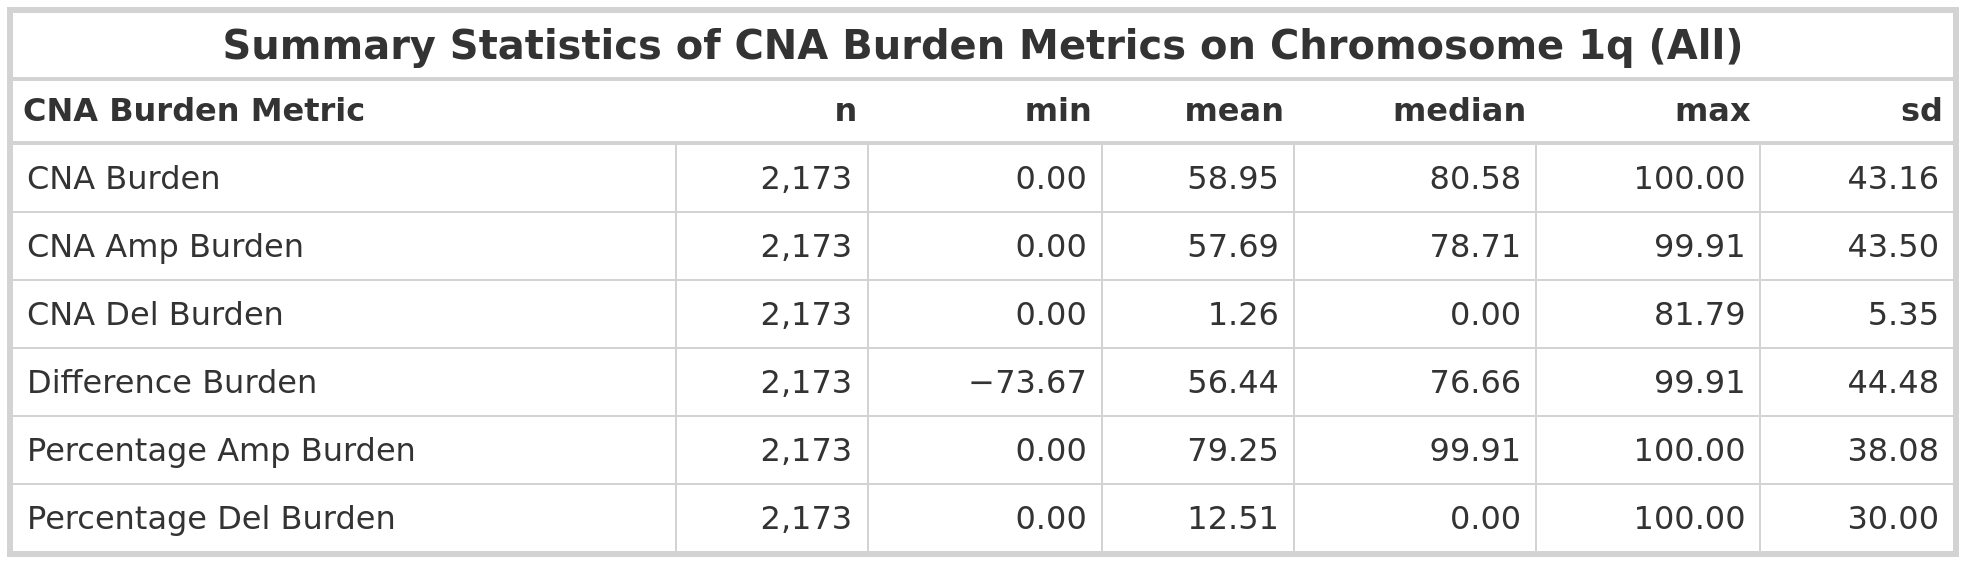
\includegraphics[width = 0.98\textwidth]{../tables/Chapter_2/CNA_Burden_Metric_All_Chr1q_Summary.png}
\label{tab:Burden_All_Chr1q}
\end{table}

\begin{table}[!ht]
\center
\caption[Summary statistics of the CNA Burden metrics on chromosome 1q where only complete cases are used.]{Summary statistics of the CNA Burden metrics on chromosome 1q where only complete cases are used.}
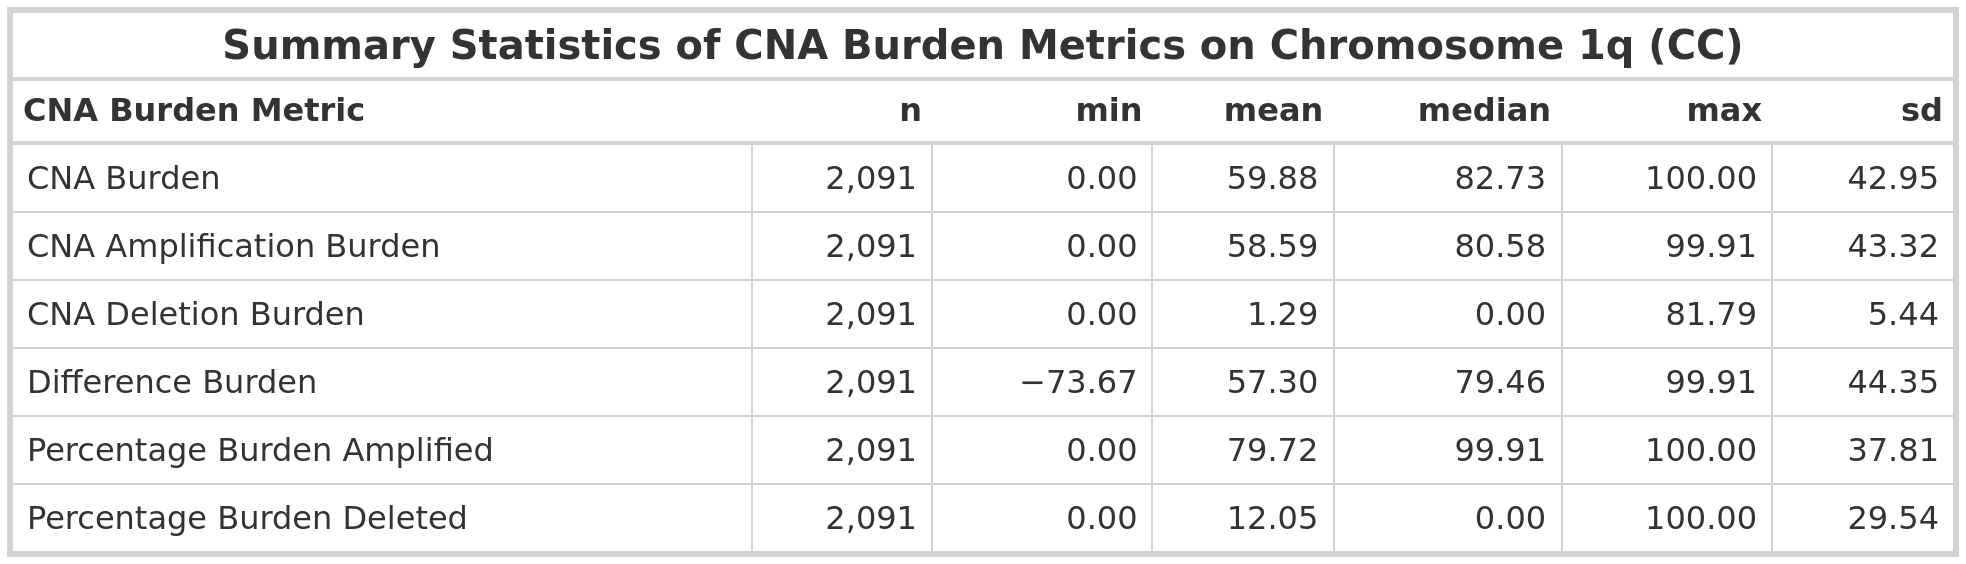
\includegraphics[width = 0.98\textwidth]{../tables/Chapter_2/CNA_Burden_Metric_CCA_Chr1q_Summary.png}
\label{tab:Burden_CCA_Chr1q}
\end{table}

\begin{figure}[!ht]
\center
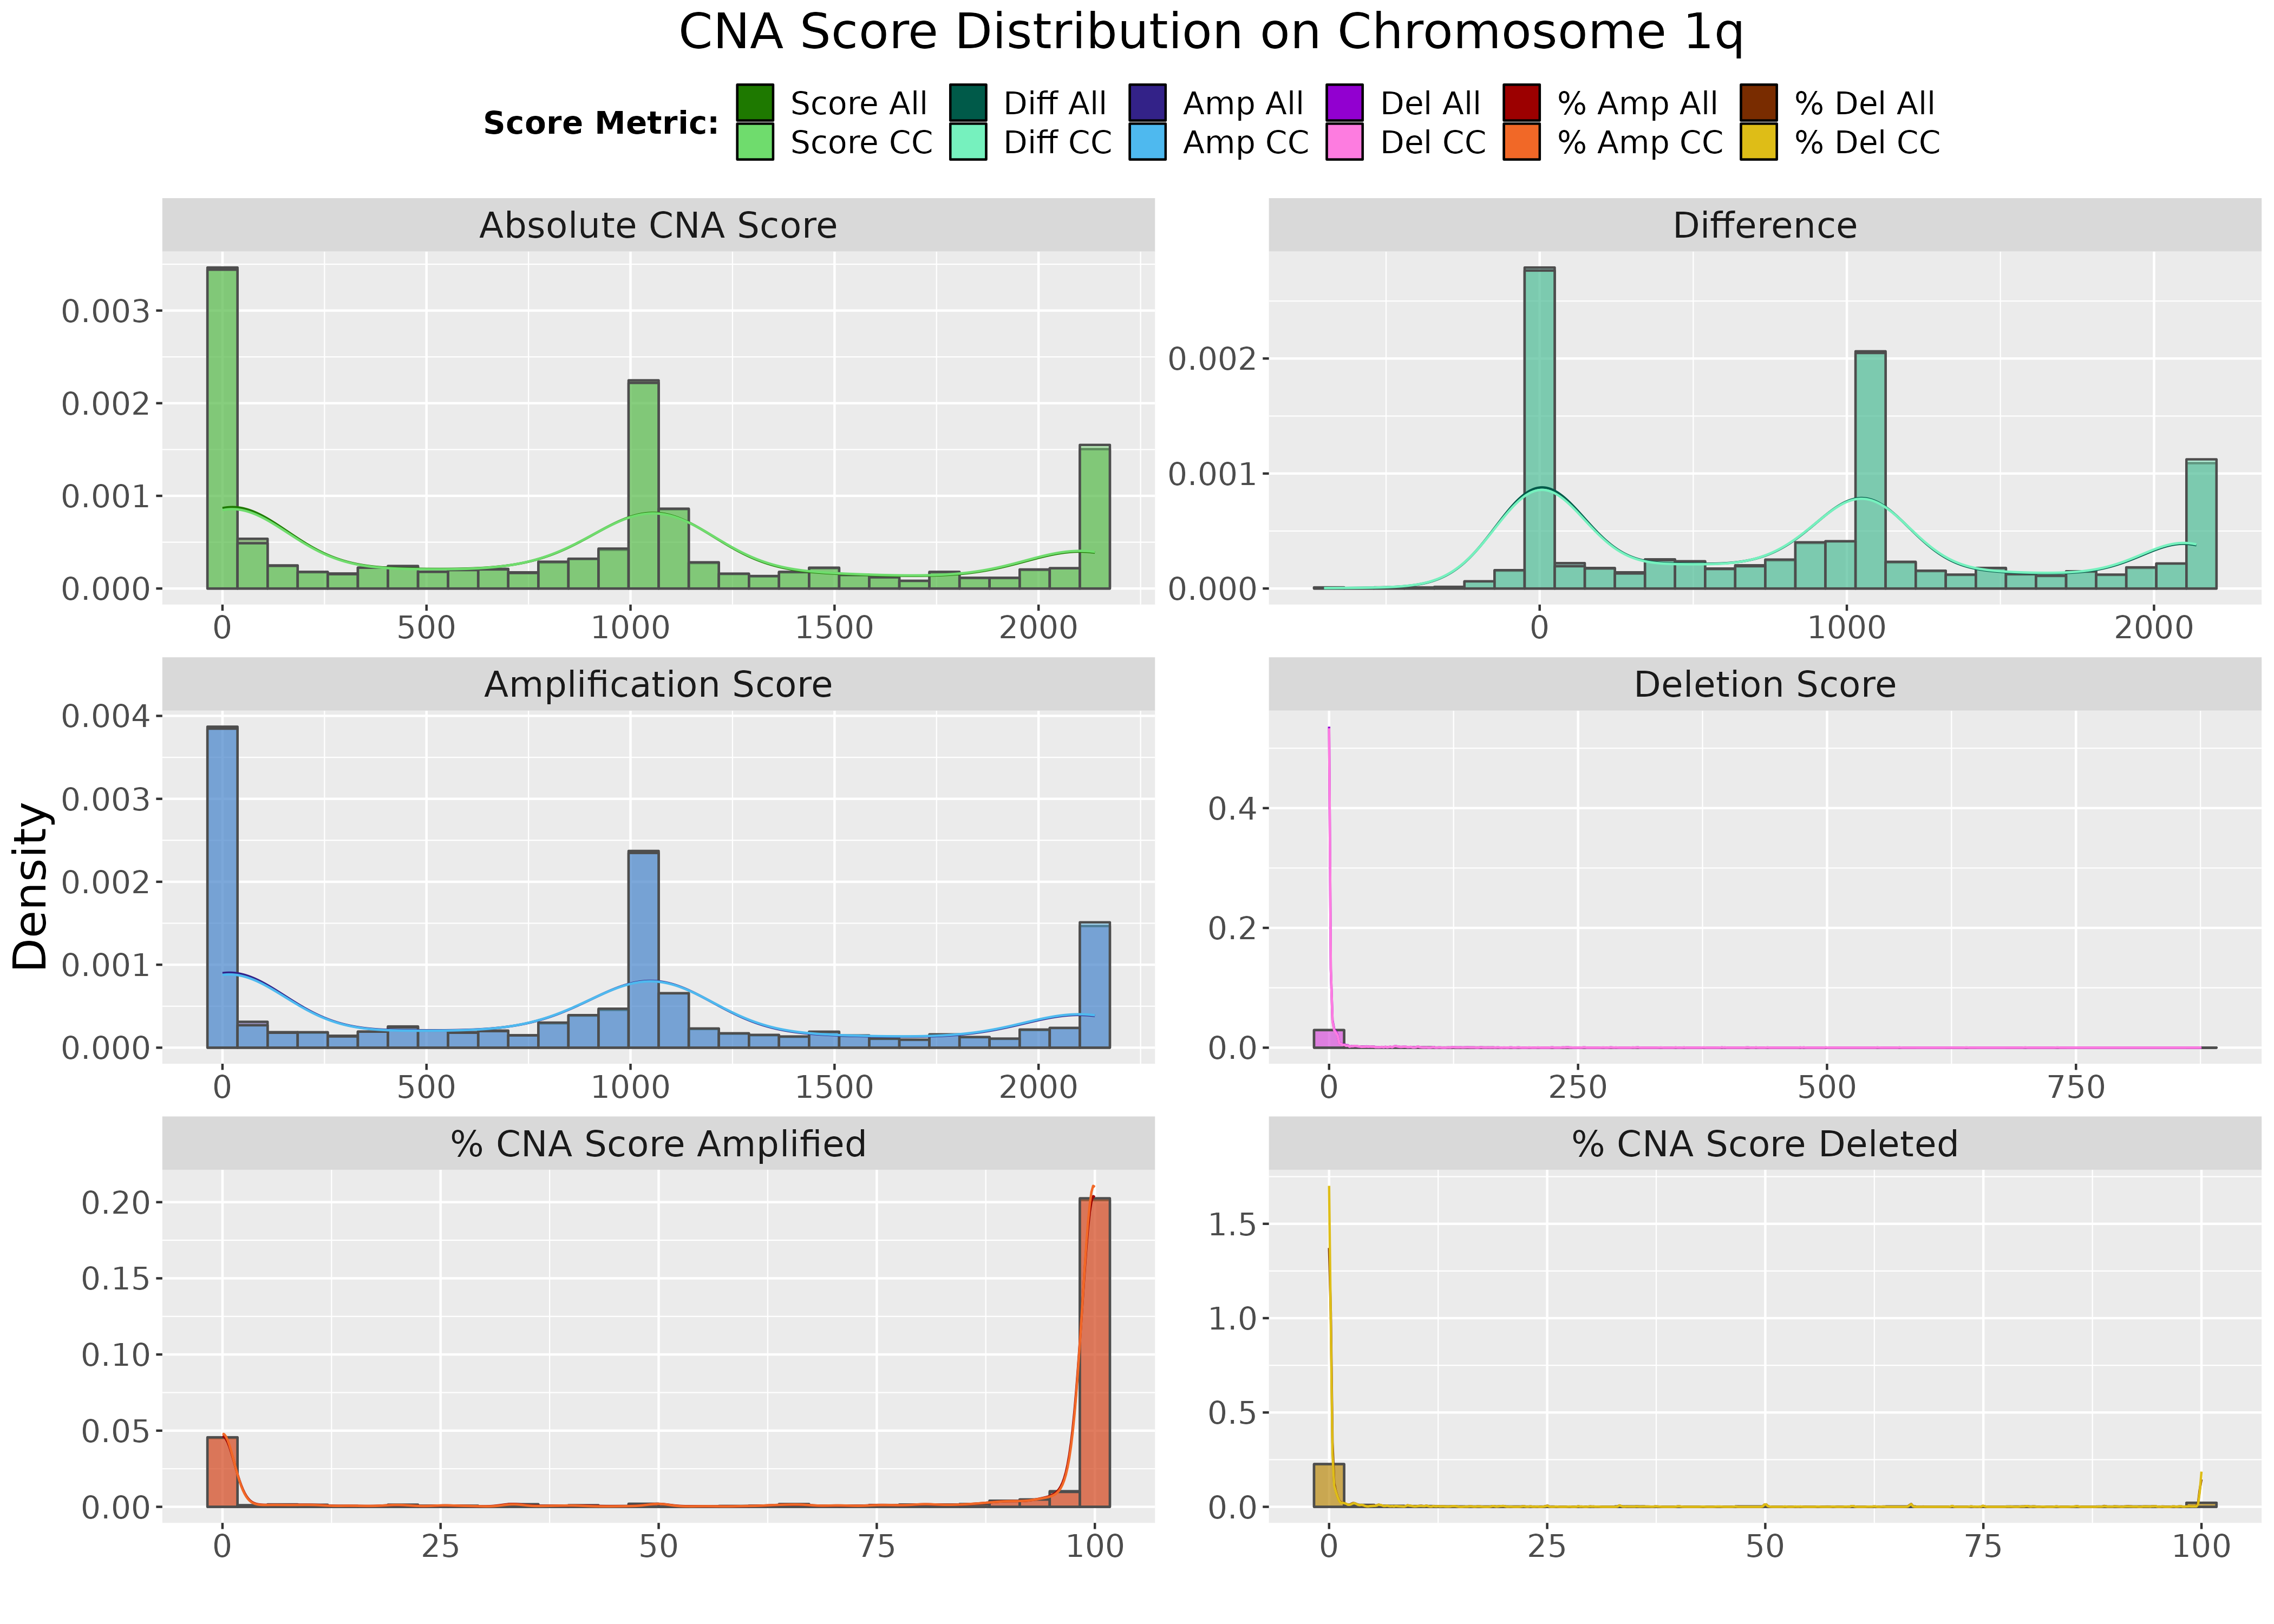
\includegraphics[width = 0.96\textwidth]{../figures/Chapter_2/CNA_Score_Comparative_Density_Chr1q.png}
\caption[Density plots for each CNA Score metric on chromosome 1q.]{Density plots for each CNA Score metric on chromosome 1q. Each facet contains density plots for both the complete-case CNA Score metric and the CNA Score metric calculated using all available data.}
\label{fig:Score_Comp_Dense_Chr1q}
\end{figure}

\begin{figure}[!ht]
\center
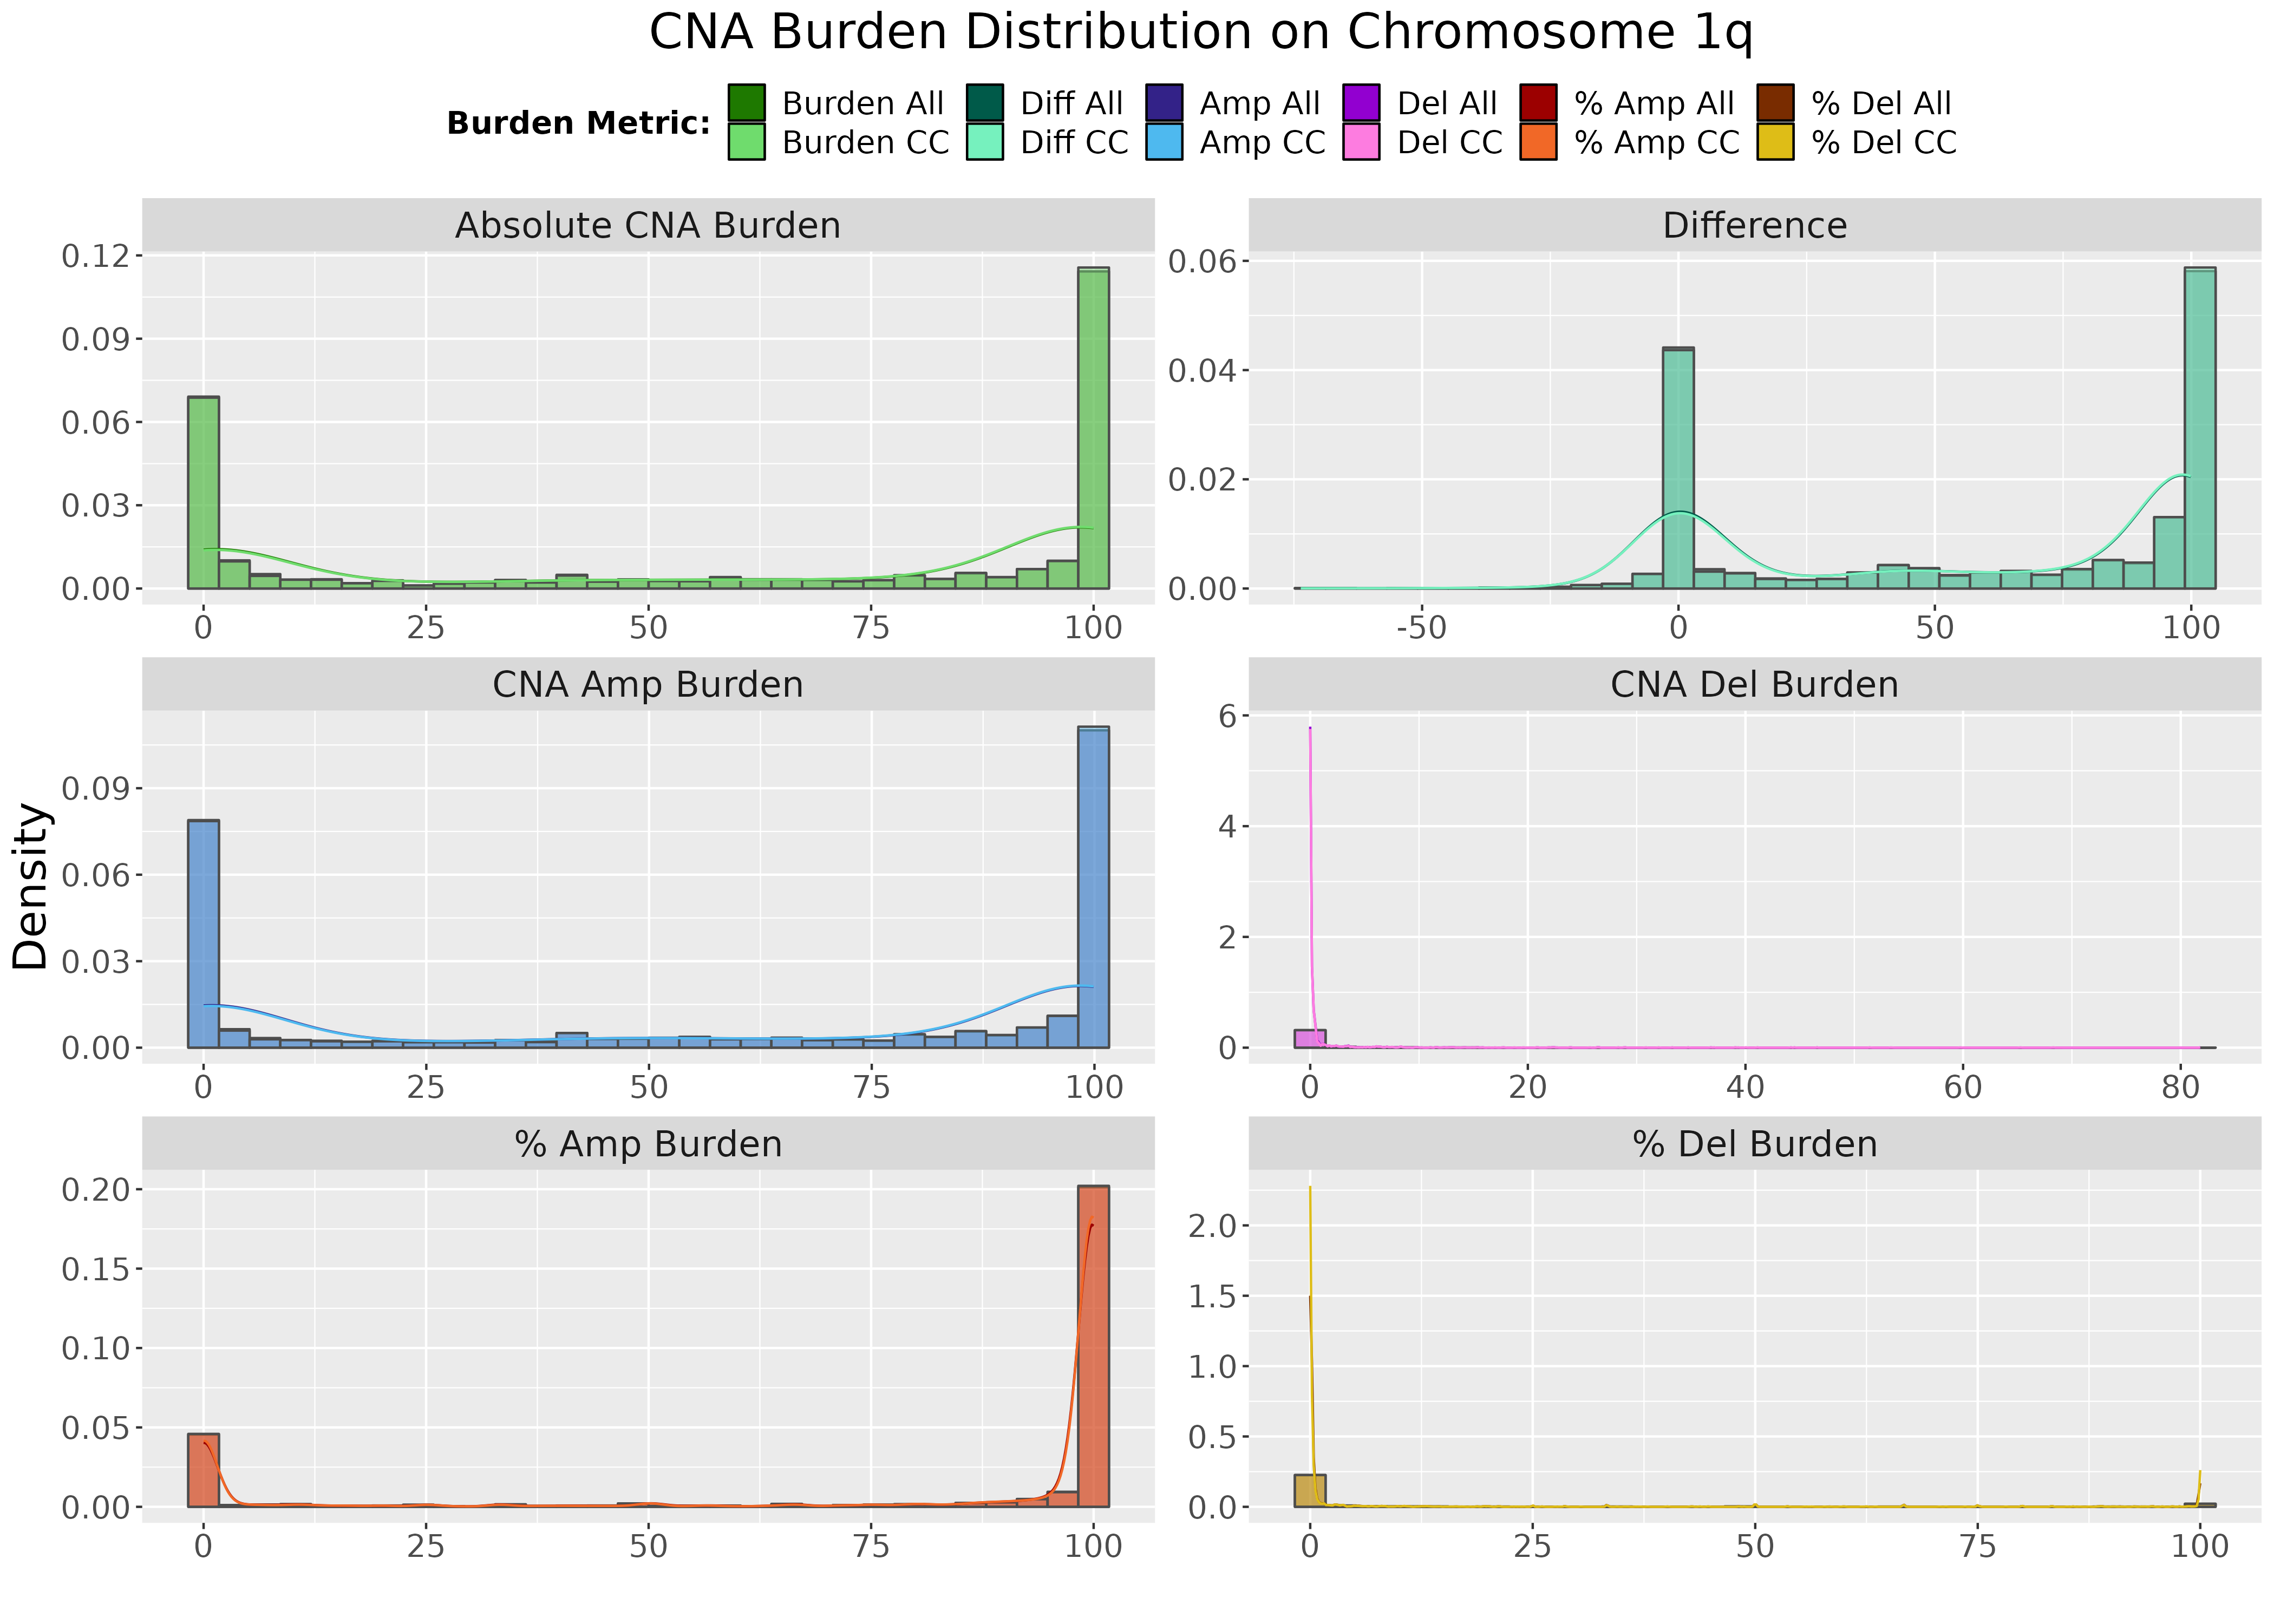
\includegraphics[width = 0.96\textwidth]{../figures/Chapter_2/CNA_Burden_Comparative_Density_Chr1q.png}
\caption[Density plots for each CNA Burden metric on chromosome 1q.]{Density plots for each CNA Burden metric on chromosome 1q. Each facet contains density plots for both the complete-case CNA Burden metric and the CNA Burden metric calculated using all available data.}
\label{fig:Burden_Comp_Dense_Chr1q}
\end{figure}
\clearpage 

\subsection{CNA Metric Distributions within Molecular Subtype Classifications}
\label{LGI}
The calculated CNA Score and Burden metrics are cross-referenced against breast cancer subtype classifications, PAM50 subtype and IntClust, to determine if observed distributions of metrics differed comparing these stratified cohorts of patients. Within the METABRIC cohort there are 1,974 patients for which CNA data and PAM50 subtype information are available and 1,980 patients for which CNA data and IntClust information are available (Table \ref{Clinchar}). The 529 patients missing both PAM50 and IntClust information did not have any gene expression data available meaning they could not be allocated PAM50 or IntClust, while six patients had IntClust information but were categorised as PAM50 “NC” and subsequently recoded as NA. We present distributions of the global CNA metrics across molecular classifications in Section \ref{ObsDis} and distributions of the chromosome arm CNA metrics across molecular classifications in Section \ref{ObsDis1}.

\subsubsection{Observed Distributions for Global CNA Metrics across Molecular Subtype Classifications}
\label{ObsDis}
The observed distribution of the six CNA Score metrics, for patients stratified by PAM50 subtype, is displayed in Figure \ref{fig:CNA-Score-Metric-Boxplots-P50}, and Figure \ref{fig:CNA-Burden-Metric-Boxplots-P50} displays the six CNA Burden metrics. Also provided with Figures \ref{fig:CNA-Score-Metric-Boxplots-P50} and \ref{fig:CNA-Burden-Metric-Boxplots-P50} are the Benjamini-Hochberg (BH) adjusted p-values for the Kruskal-Wallis test for any difference in the distribution of a metric comparing the groups of patients stratified by PAM50 subtype. 

These visualisations and accompanying statistical tests (Figure \ref{fig:CNA-Score-Metric-Boxplots-P50} and Figure \ref{fig:CNA-Burden-Metric-Boxplots-P50}) indicate that some significant difference exists comparing each of the CNA metric distributions across PAM50 subtype (Kruskal-Wallis adjusted $p<0.0001$). Dunn's Test, a post-hoc test for Kruskal-Wallis, is then applied to each CNA metric performing pairwise comparisons to determine which groups are significantly different in mean rank scores (Tables \ref{tab:DT_Score_1} and \ref{tab:DT_Burden_1}). The distribution of CNA Score and Burden metrics in Basal patients is significantly different from all other subtypes (Tables \ref{tab:DT_Score_1} and \ref{tab:DT_Burden_1}). Basal patients display the highest Absolute CNA Scores and CNA Burden across all subtypes ($p<0.0001$) indicating higher levels of GI when compared to other subtypes. In line with this, the Basal patients display the highest CNA Amp and Del Score and Burden across all subtypes ($p<0.001$ for each comparison).

The HER2 and Luminal B subtypes have the 2nd and 3rd highest Absolute CNA Score and Burden, CNA Amp Score and Burden and CNA Del Score and Burden, respectively. While the shape and spread of these metric distributions appear quite similar, the HER2 subtype displays slightly higher levels of Absolute CNA Score and Burden ($p = 0.01$). This is also observed for the CNA Del metrics, where HER2 patients have higher levels of deletions than Luminal B patients ($p = 0.01$), but not the CNA Amp metrics ($p = 0.41$ and $p = 0.47$). When comparing the Luminal A and Luminal B patients, it is observed that Luminal B patients have significantly higher levels of instability across all metrics ($p<0.0001$). The Luminal A, Normal and Claudin-low patients display the lowest CNA Score and Burden metrics. The Normal and Claudin-low subtypes display no significant difference for the total, amplification and deletion CNA Score and Burden metrics ($p>0.05$). All Luminal A and Claudin-low densities, apart from the CNA Amp metric distributions, are not significantly different from each other in these subtypes ($p>0.05$). Luminal A patients display significantly higher levels of amplifications when compared with Normal and Claudin-low subtypes ($p < 0.0001$, Tables \ref{tab:DT_Score_1} and \ref{tab:DT_Burden_1}). 

Focusing on the direct comparison of levels of amplification to deletion within each PAM50 subtype, Figures \ref{fig:CNA-Score-Metric-Boxplots-P50-AmpDel} and \ref{fig:CNA-Burden-Metric-Boxplots-P50-AmpDel}, the subtypes known to be associated with poorer survival outcome, i.e. Basal, HER2 and Luminal B, have significantly higher levels of deletion burden than amplification burden ($p<0.0001$). Conversely PAM50 subtypes with better survival prognosis either display significantly more amplifications, Luminal A ($p < 0.01$), or no significant difference in the levels of amplifications and deletions, Normal and Claudin-low ($p > 0.05$).

\vfill
\begin{figure}[!h]
\center
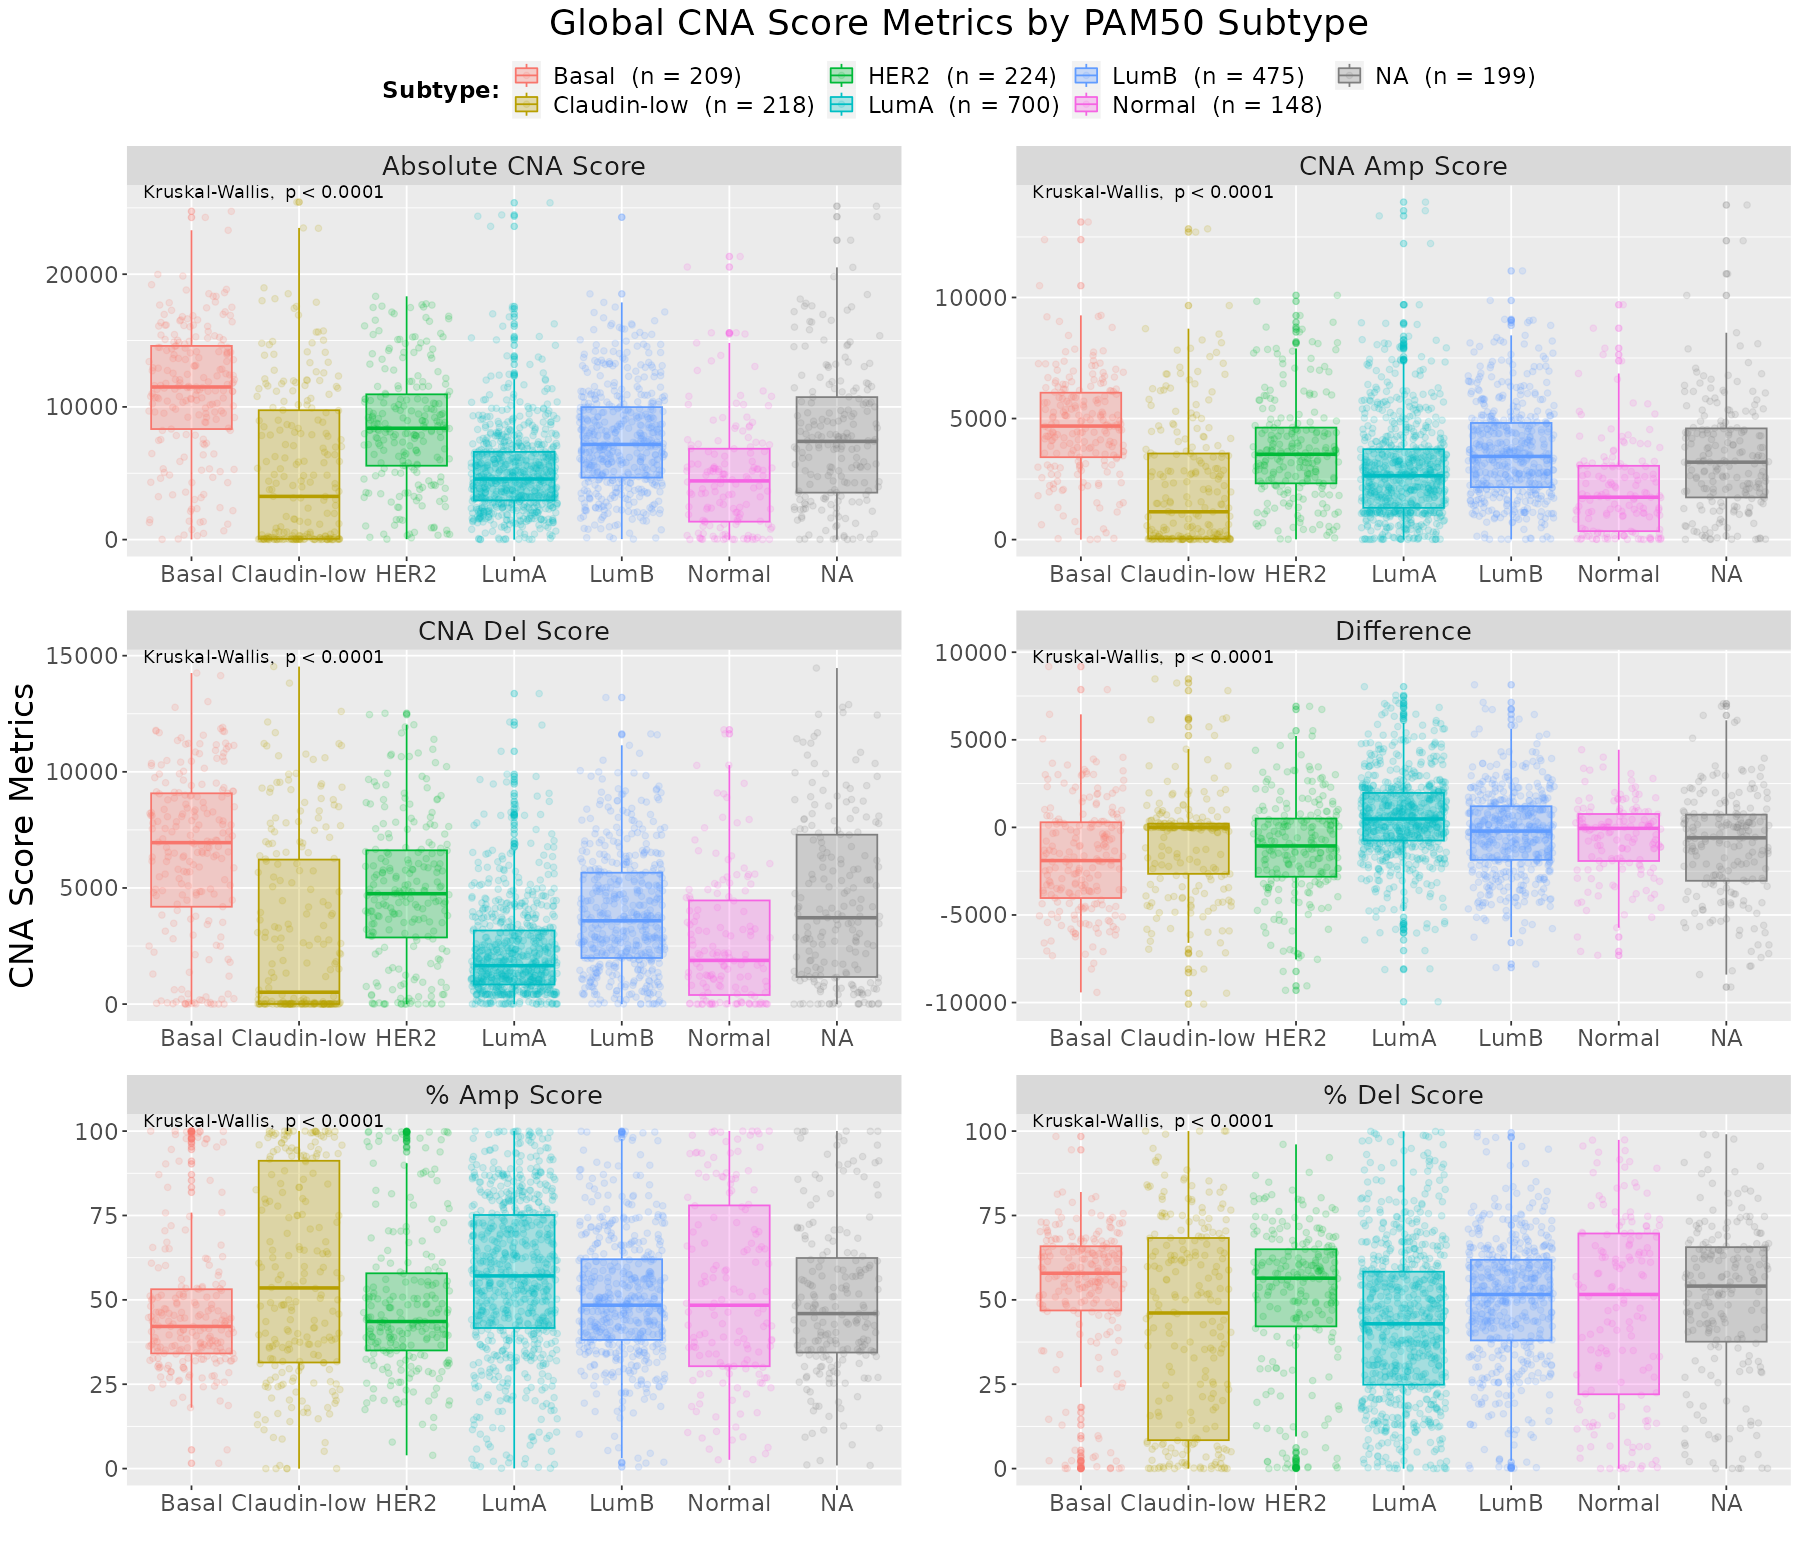
\includegraphics[width=1\textwidth]{../figures/Chapter_2/Global_CNA_Score_Metrics_Across_PAM50.png}
\caption[Boxplots for each CNA Score metric by PAM50 subtype.]{Boxplots for each CNA Score metric by PAM50 subtype. Each facet contains boxplots for the CNA Score metrics calculated using all available data accompanied by Benjamini-Hochberg adjusted Kruskal-Wallis p-values. NA denotes METABRIC patients missing PAM50 information.}
\label{fig:CNA-Score-Metric-Boxplots-P50}
\end{figure}
\vfill

\begin{figure}[!ht]
\center
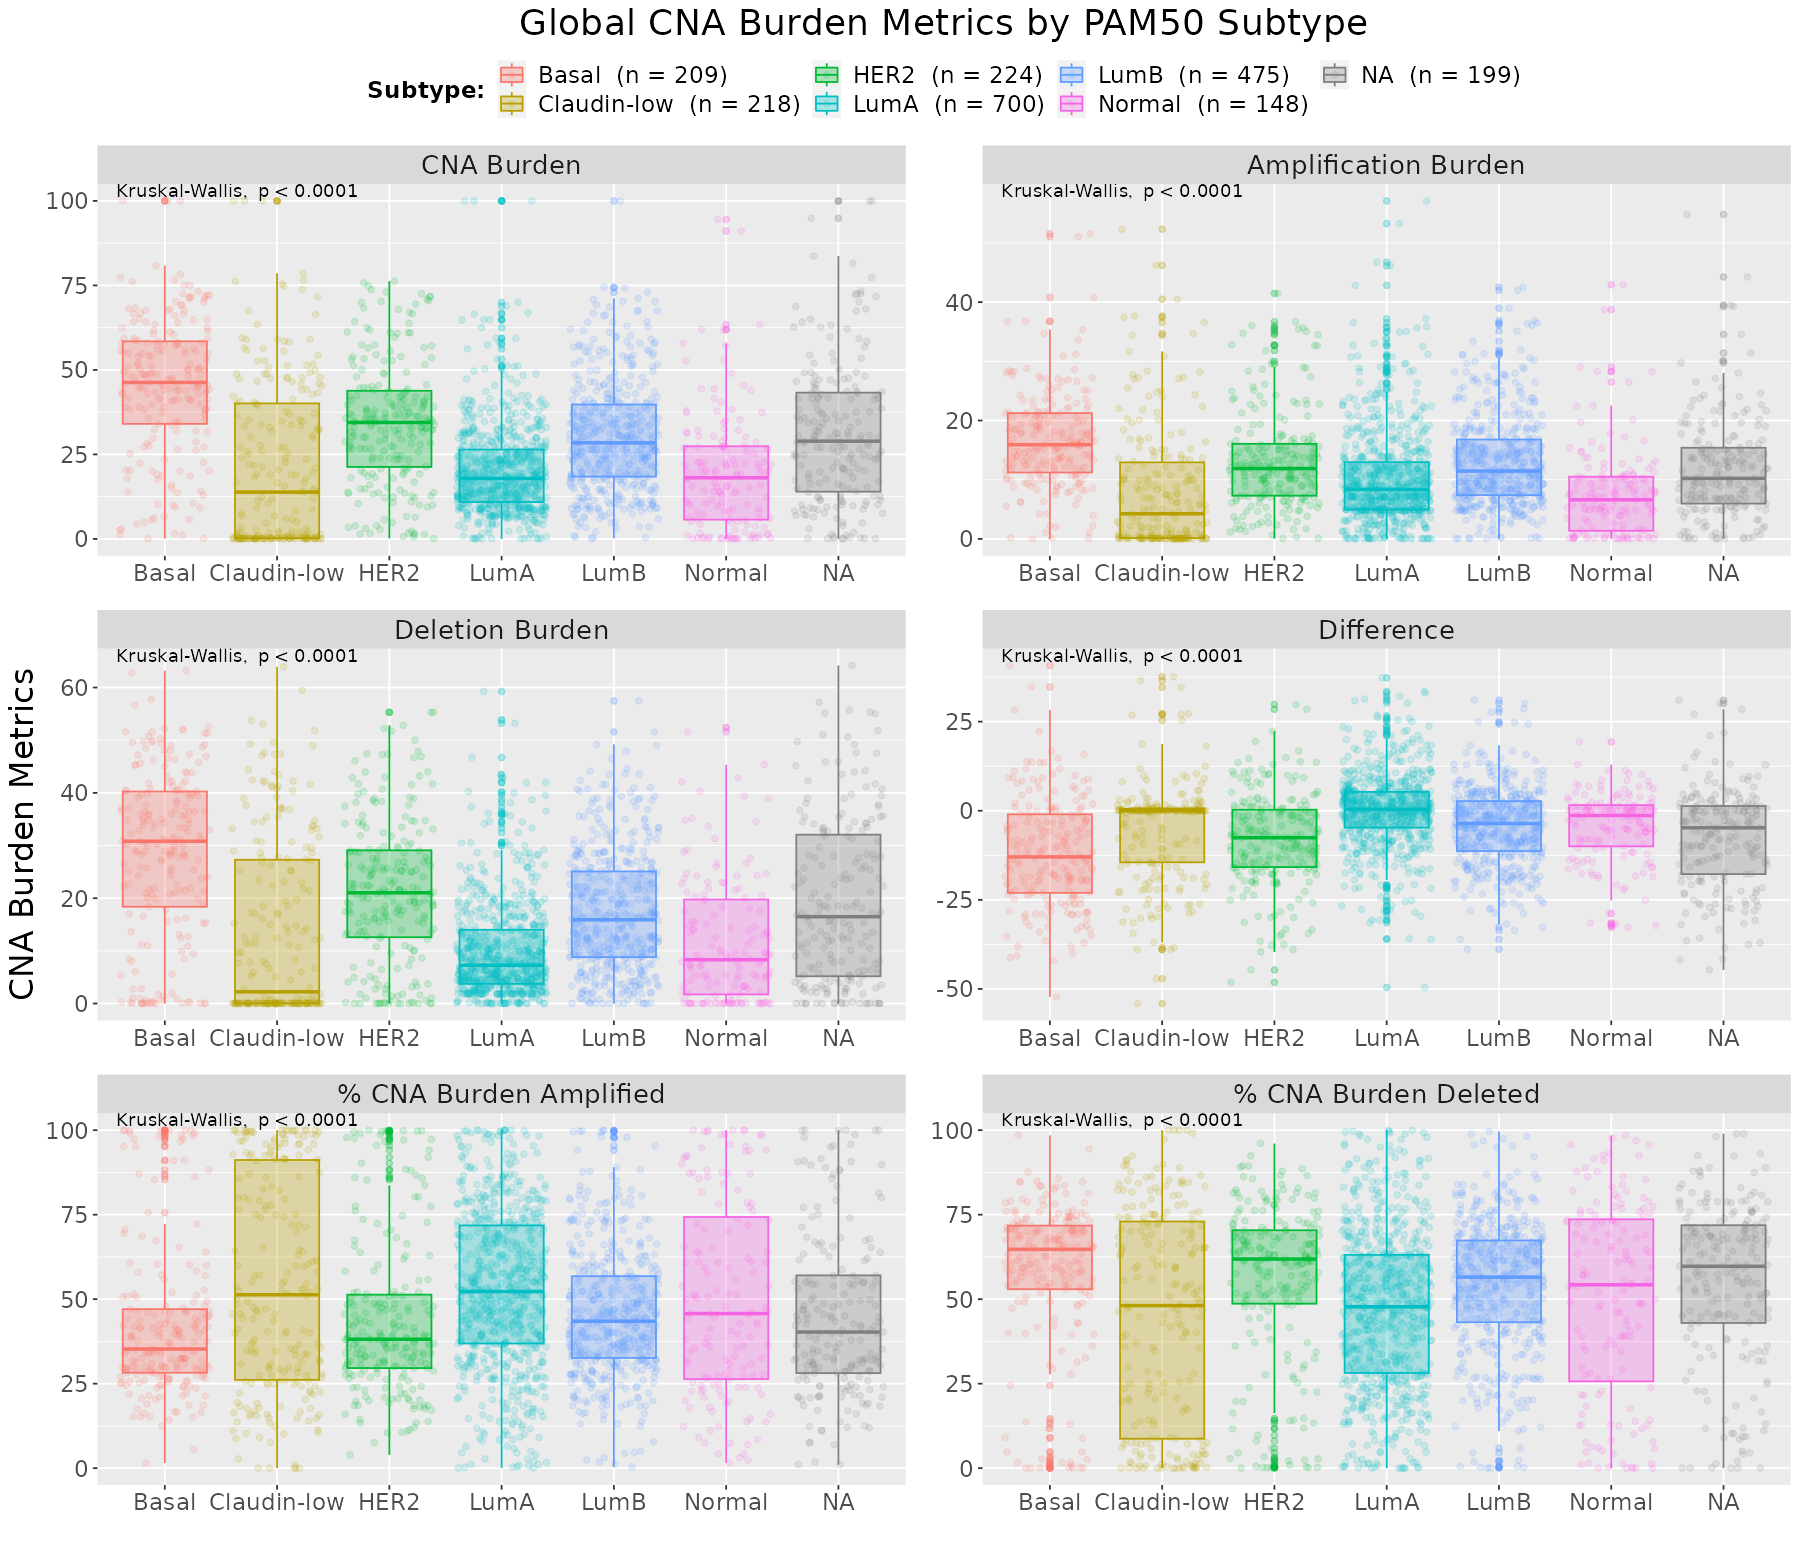
\includegraphics[width=1\textwidth]{../figures/Chapter_2/Global_CNA_Burden_Metrics_Across_PAM50.png}
\caption[Boxplots for each CNA Burden metric by PAM50 subtype.]{Boxplots for each CNA Burden metric by PAM50 subtype. Each facet contains boxplots for the CNA Burden metrics calculated using all available data accompanied by Benjamini-Hochberg adjusted Kruskal-Wallis p-values. NA denotes METABRIC patients missing PAM50 information.}
\label{fig:CNA-Burden-Metric-Boxplots-P50}
\end{figure}

\begin{table}[!ht]
\center
\caption[Comparisons of CNA Score metric distributions by PAM50 subtype.]{Comparisons of CNA Score metric distributions by PAM50 subtype. Z statistic and Benjamini-Hochberg adjusted p-value for each Dunn's test are shown.}
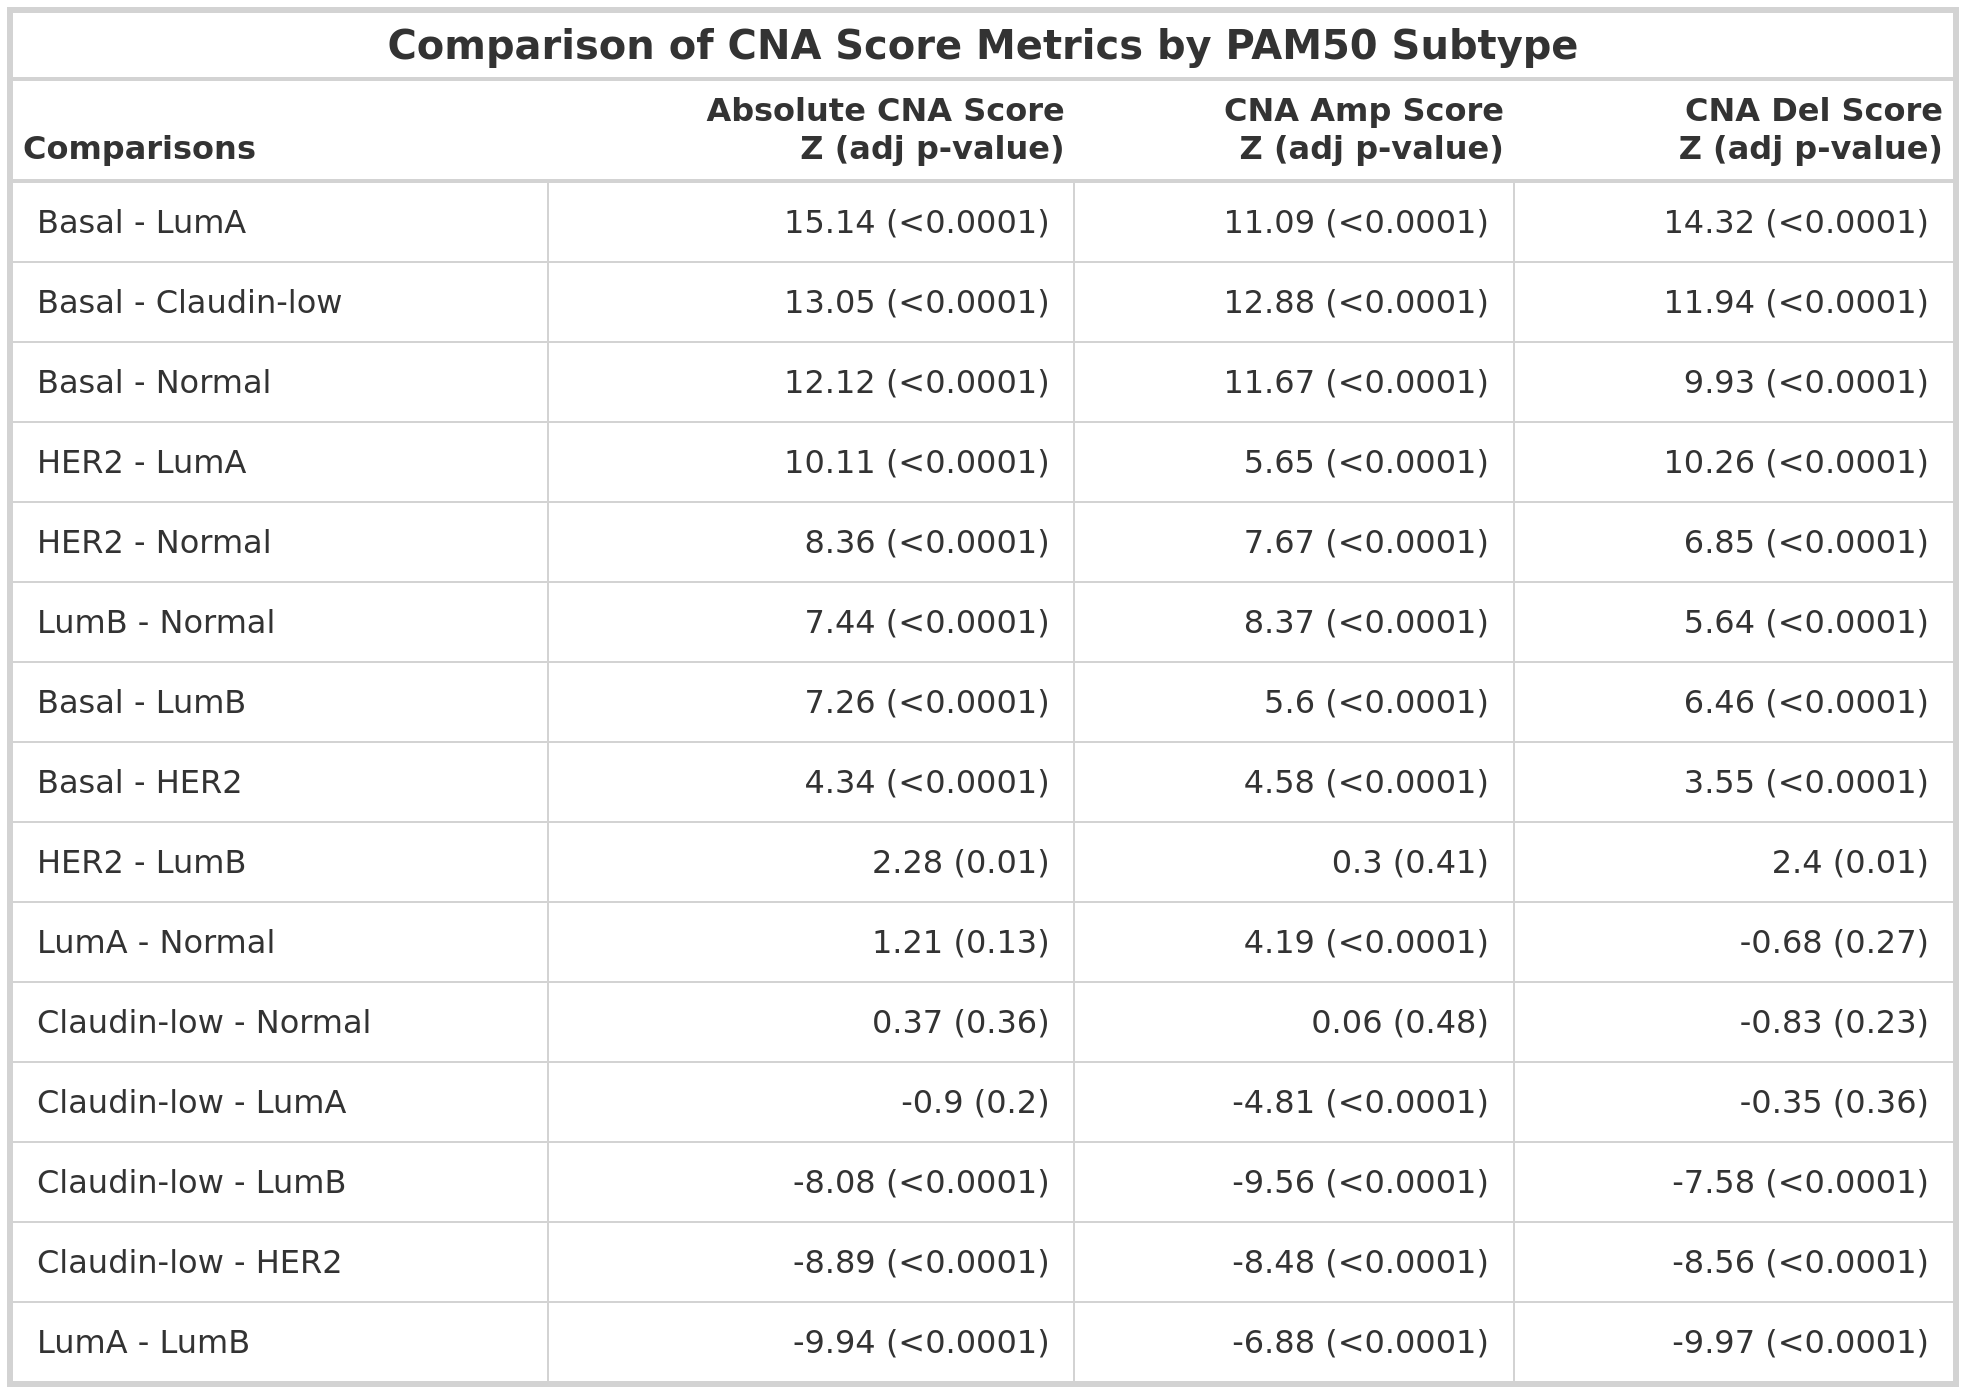
\includegraphics[width=0.98\textwidth]{../tables/Chapter_2/Global_CNA_Score_Metric_Comparisons.png}
\label{tab:DT_Score_1}
\end{table}

\begin{table}[!ht]
\center
\caption[Comparisons of CNA Burden metric distributions by PAM50 subtype.]{Comparisons of CNA Burden metric distributions by PAM50 subtype. Z statistic and Benjamini-Hochberg adjusted p-value for each Dunn's test are shown.}
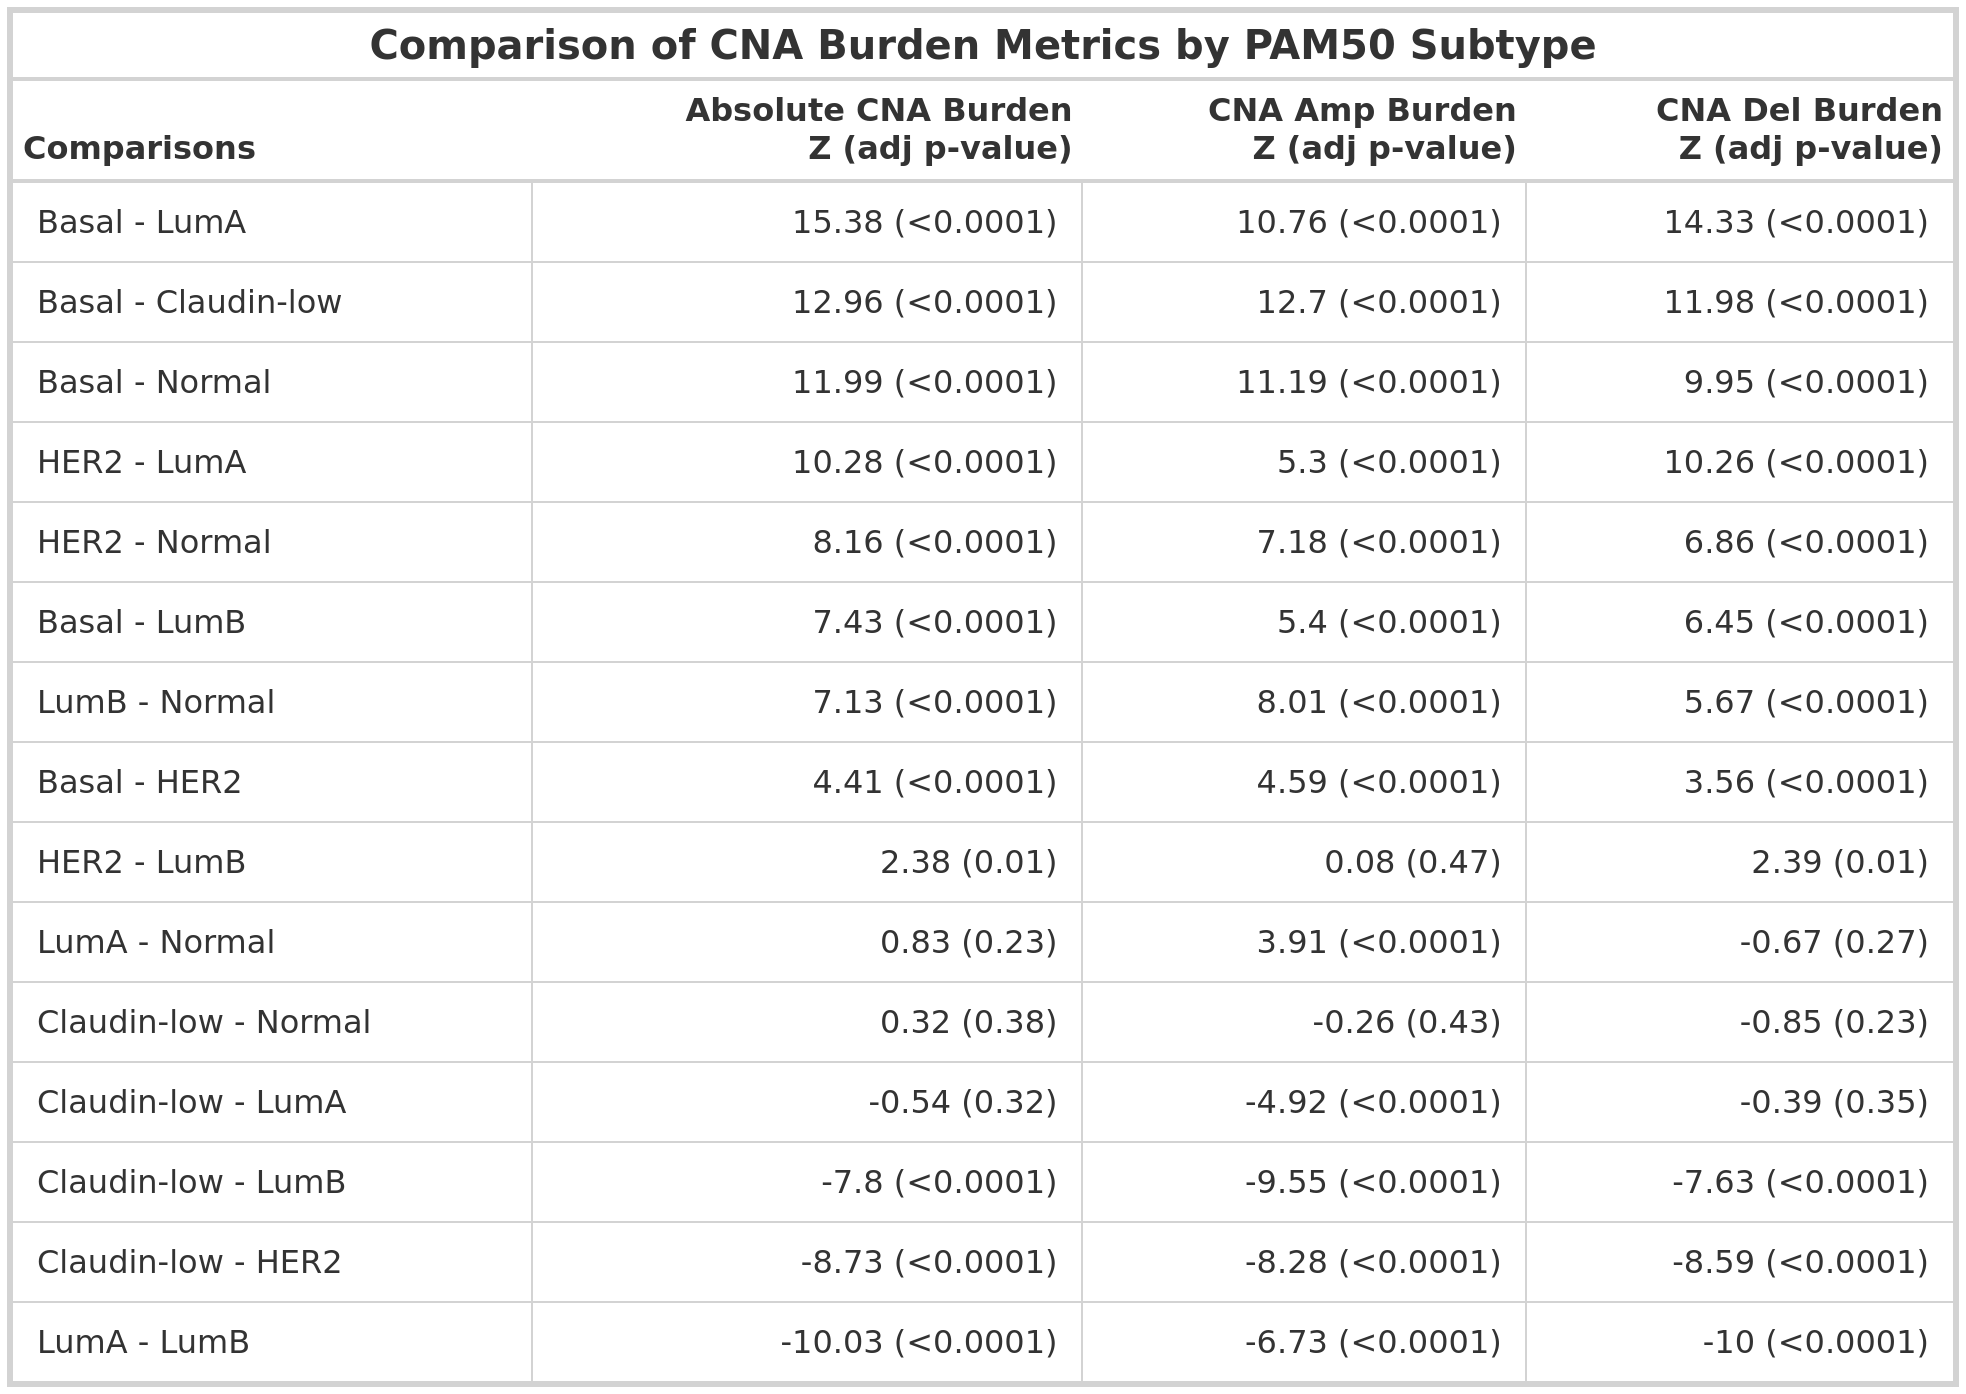
\includegraphics[width=0.98\textwidth]{../tables/Chapter_2/Global_CNA_Burden_Metric_Comparisons.png}
\label{tab:DT_Burden_1}
\end{table}

\begin{figure}[!ht]
\center
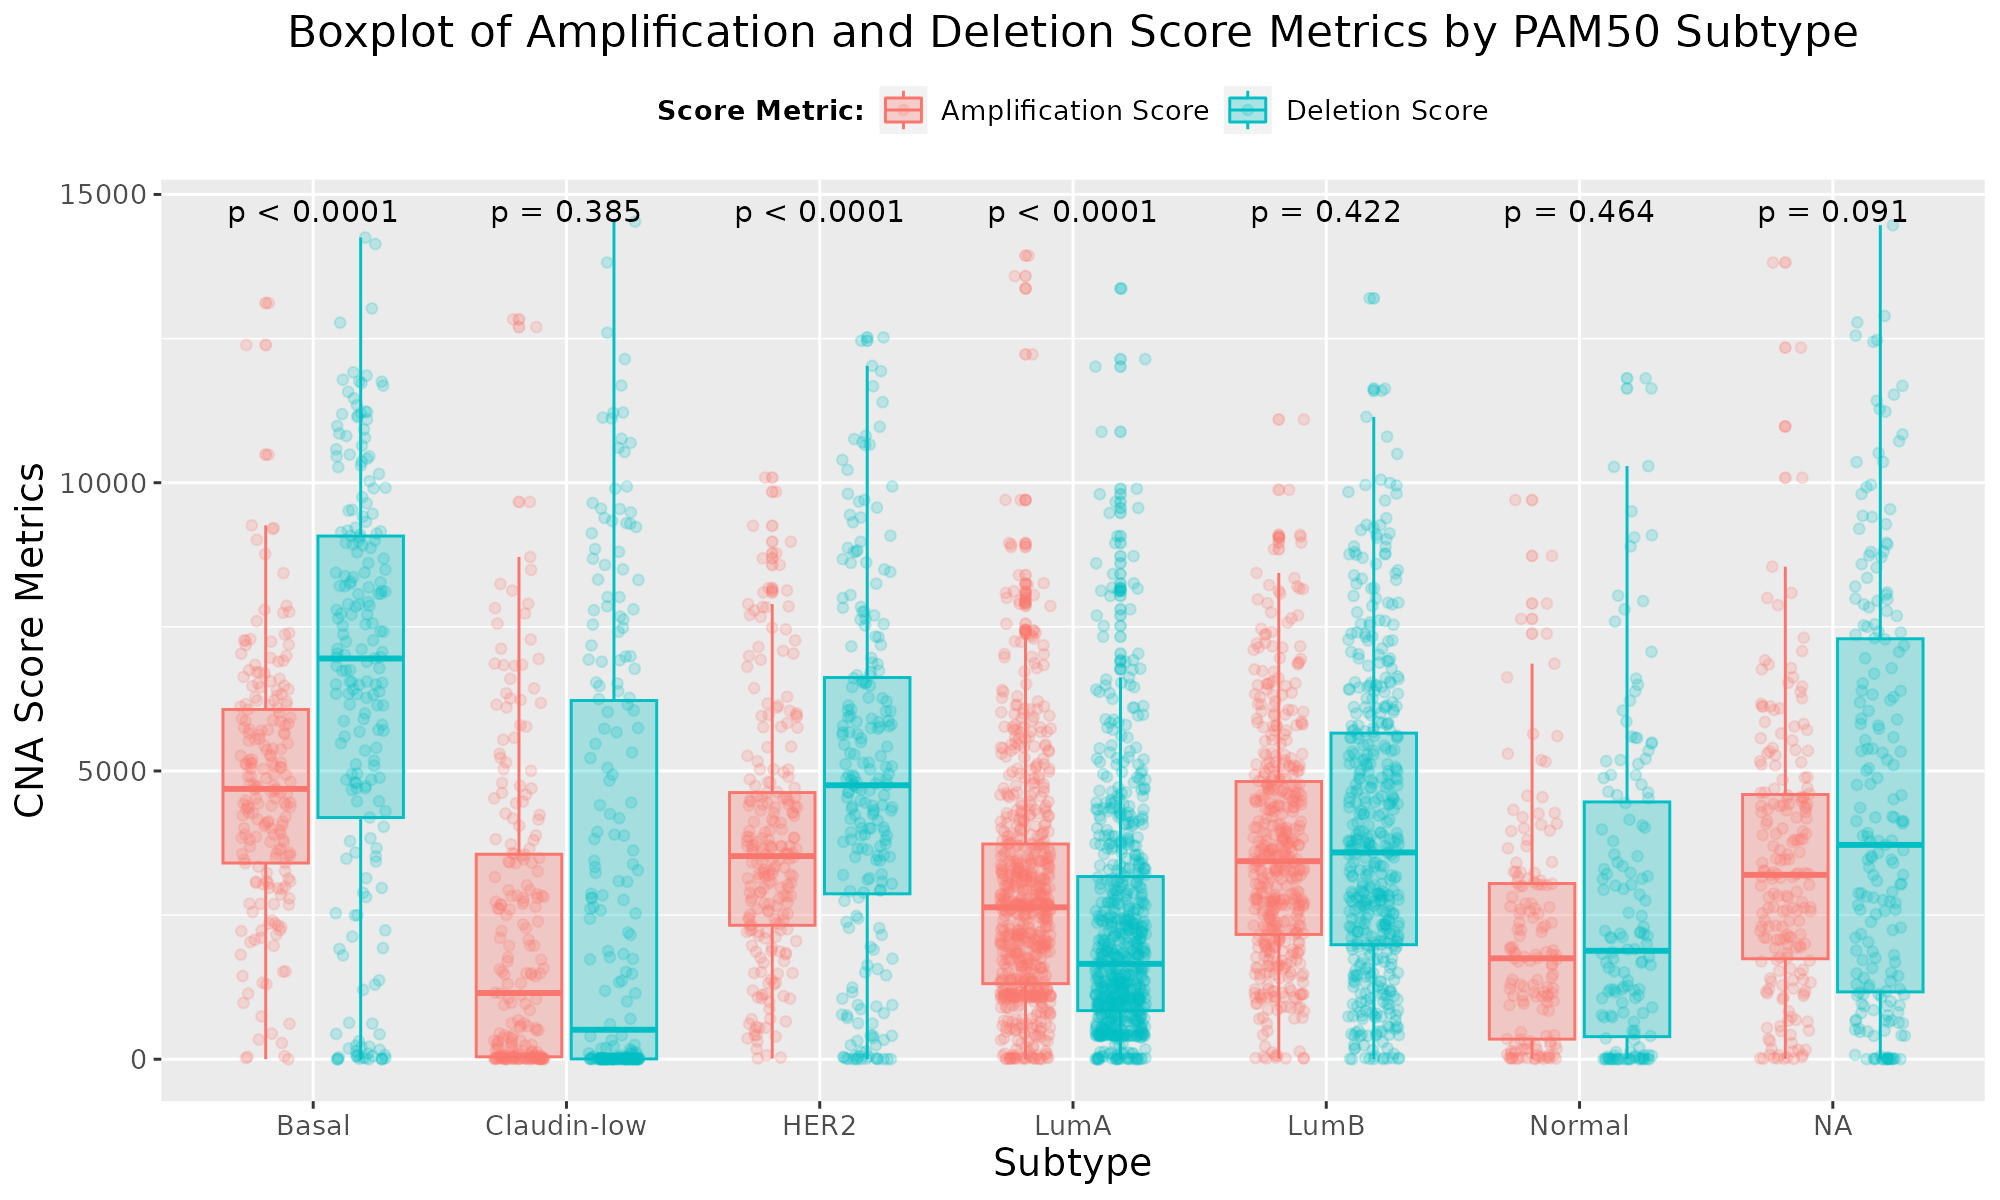
\includegraphics[width=1\textwidth]{../figures/Chapter_2/Global_CNA_Score_AmpDel_Across_PAM50.png}
\caption[Boxplots for each CNA Amp and CNA Del Score metric by PAM50 subtype.]{Boxplots for each CNA Amp and CNA Del Score metric by PAM50 subtype. Includes Benjamini-Hochberg adjusted Kruskal-Wallis p-values.}
\label{fig:CNA-Score-Metric-Boxplots-P50-AmpDel}
\end{figure}

\begin{figure}[!ht]
\center
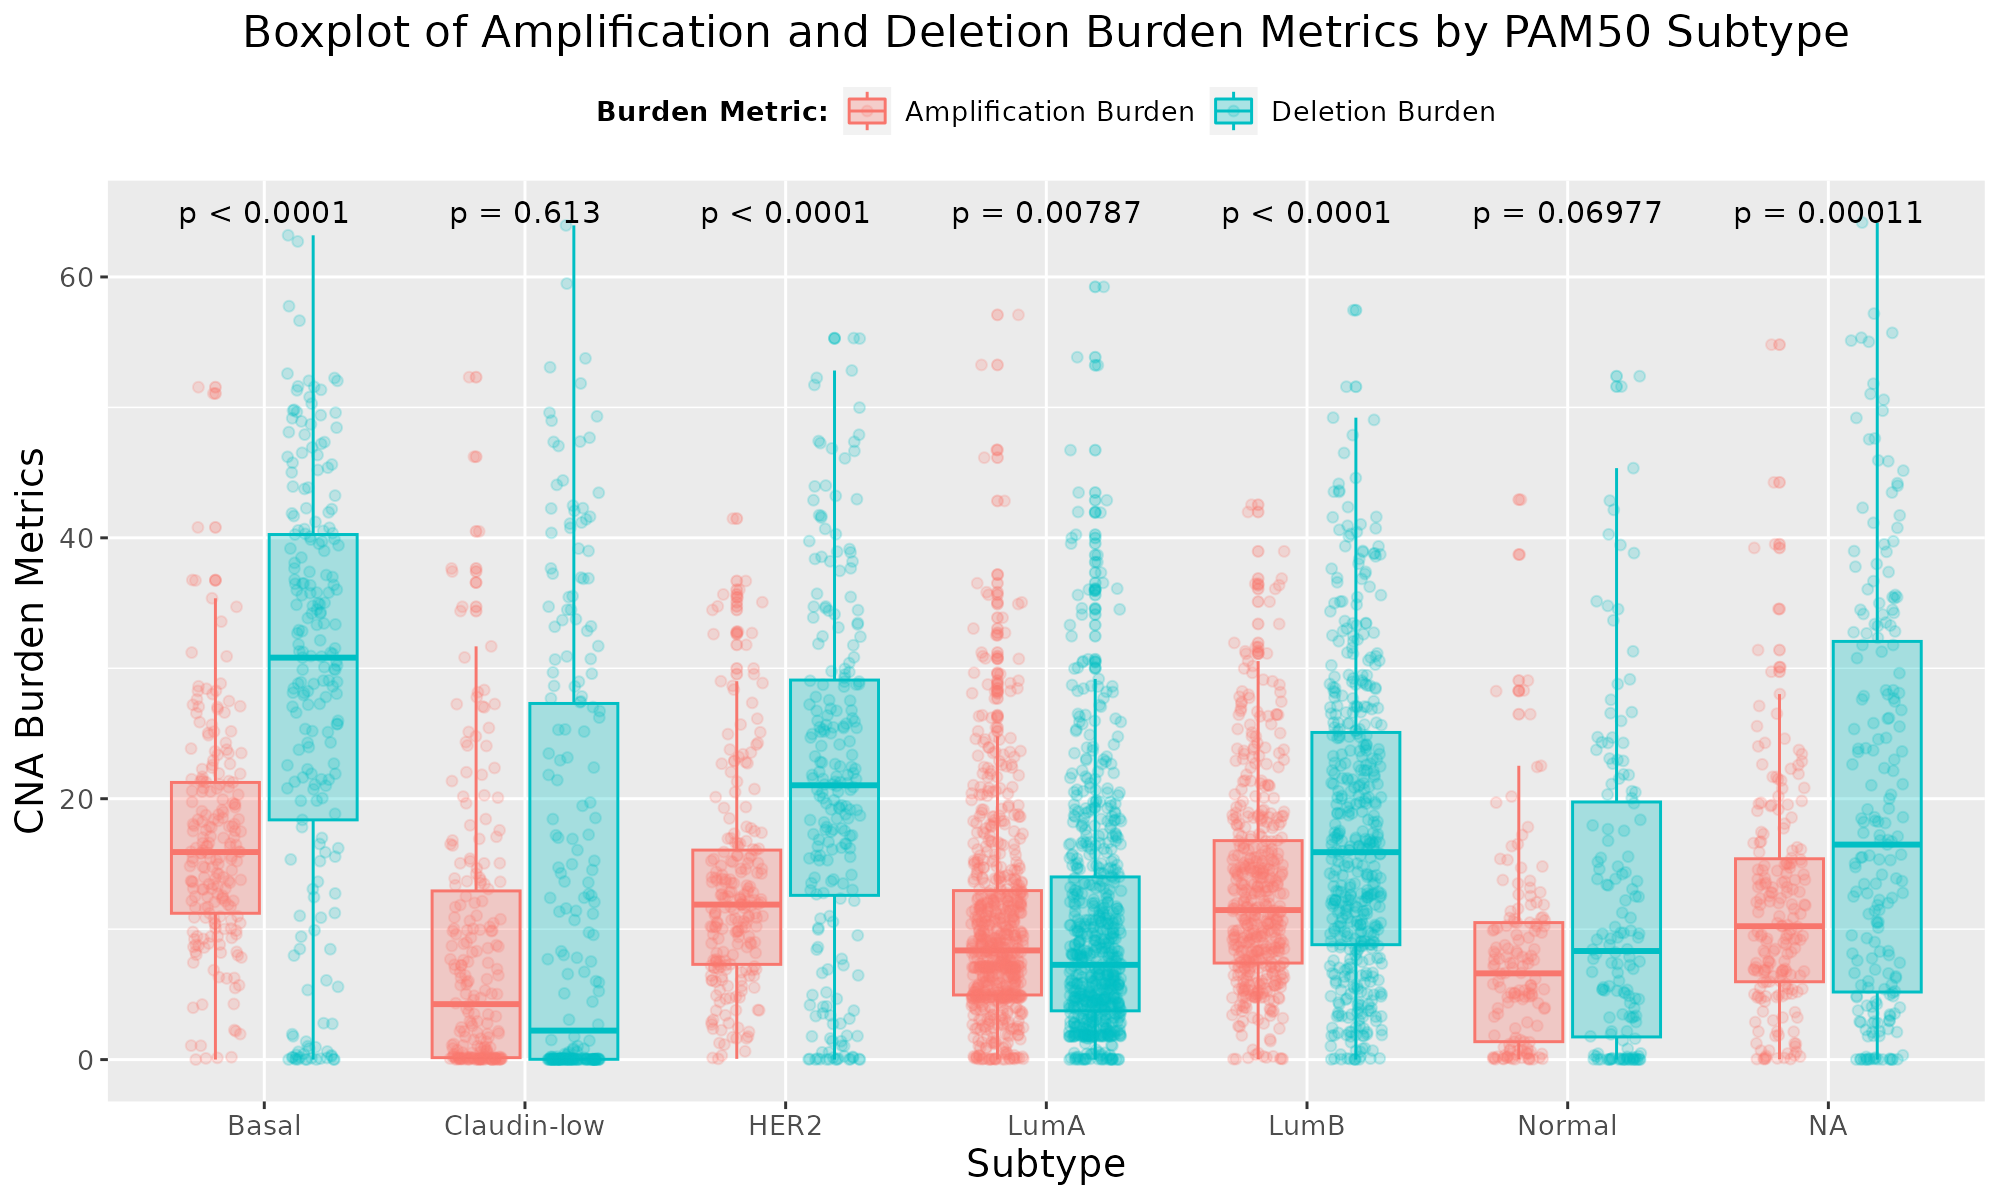
\includegraphics[width=1\textwidth]{../figures/Chapter_2/Global_CNA_Burden_AmpDel_Across_PAM50.png}
\caption[Boxplots for each CNA Amp and CNA Del Burden metric by PAM50 subtype.]{Boxplots for each CNA Amp and CNA Del Burden metric by PAM50 subtype. Includes Benjamini-Hochberg adjusted Kruskal-Wallis p-values.}
\label{fig:CNA-Burden-Metric-Boxplots-P50-AmpDel}
\end{figure}
\clearpage 

The observed distribution of the six CNA metrics, for patients stratified by IntClust is provided (Figures \ref{fig:CNA-Score-Metric-Boxplots-IC} and \ref{fig:CNA-Burden-Metric-Boxplots-IC}), accompanied by BH adjusted Kruskal-Wallis p-values. These figures indicate some significant difference exists comparing each of the CNA metric distributions across IntClusts (Kruskall-Wallis adjusted $p<0.0001$ for all CNA metrics).

\begin{figure}[!ht]
\center
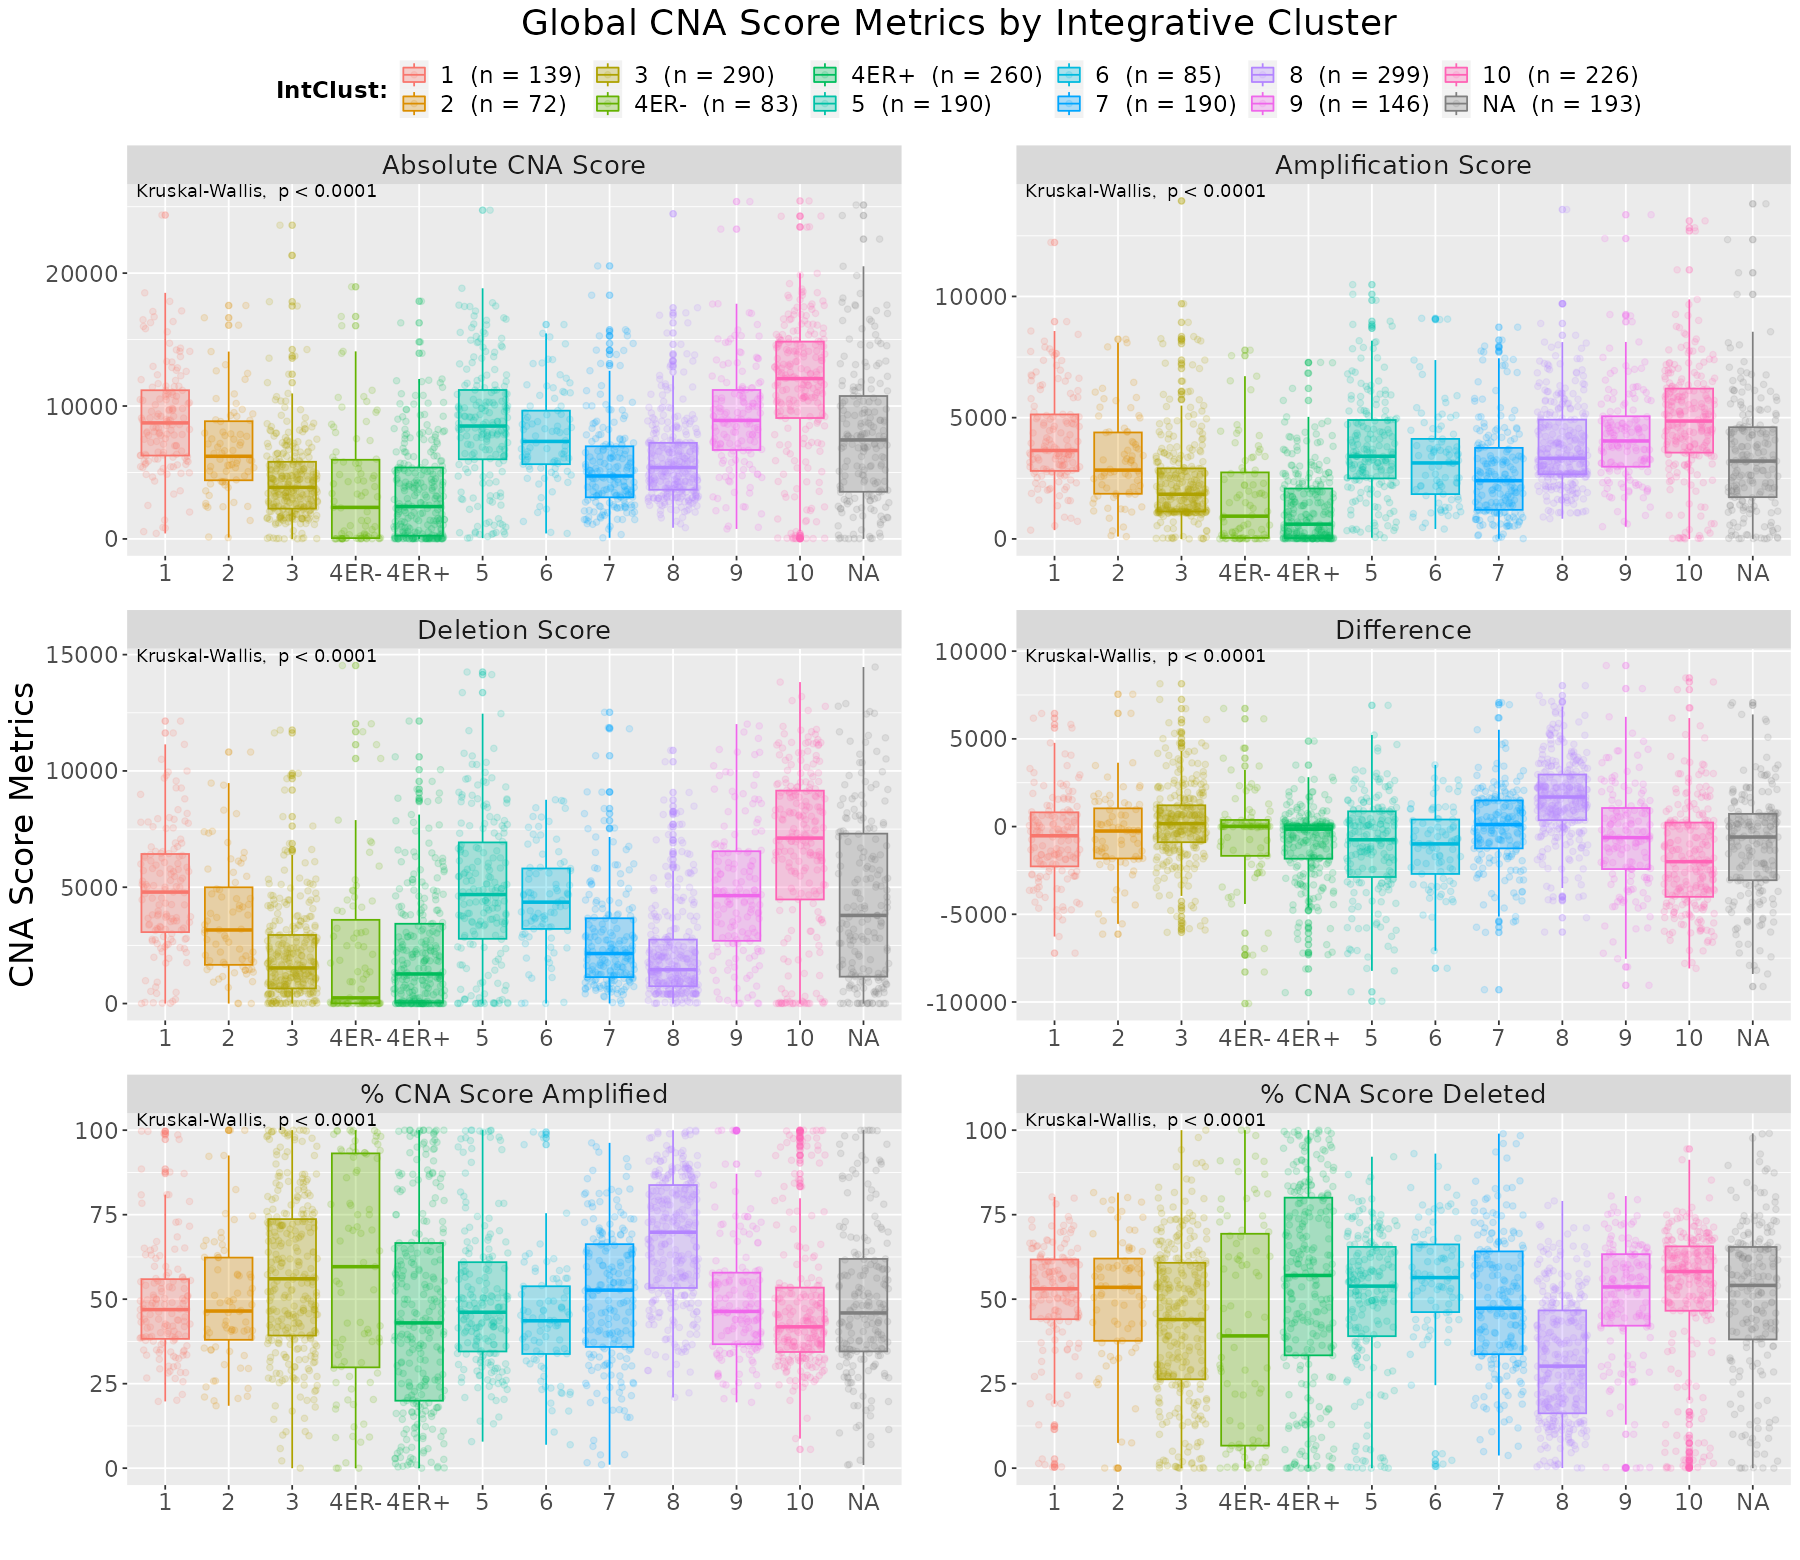
\includegraphics[width=1\textwidth]{../figures/Chapter_2/Global_CNA_Score_Metrics_Across_IntClust.png}
\caption[Boxplots for each CNA Score metric by Integrative Cluster.]{Boxplots for each CNA Score metric by Integrative Cluster. Each facet contains boxplots for the CNA Score metrics calculated using all available data and Benjamini-Hochberg adjusted Kruskal-Wallis p-values. NA denotes METABRIC patients missing Integrative Cluster information.}
\label{fig:CNA-Score-Metric-Boxplots-IC}
\end{figure}

\begin{figure}[!ht]
\center
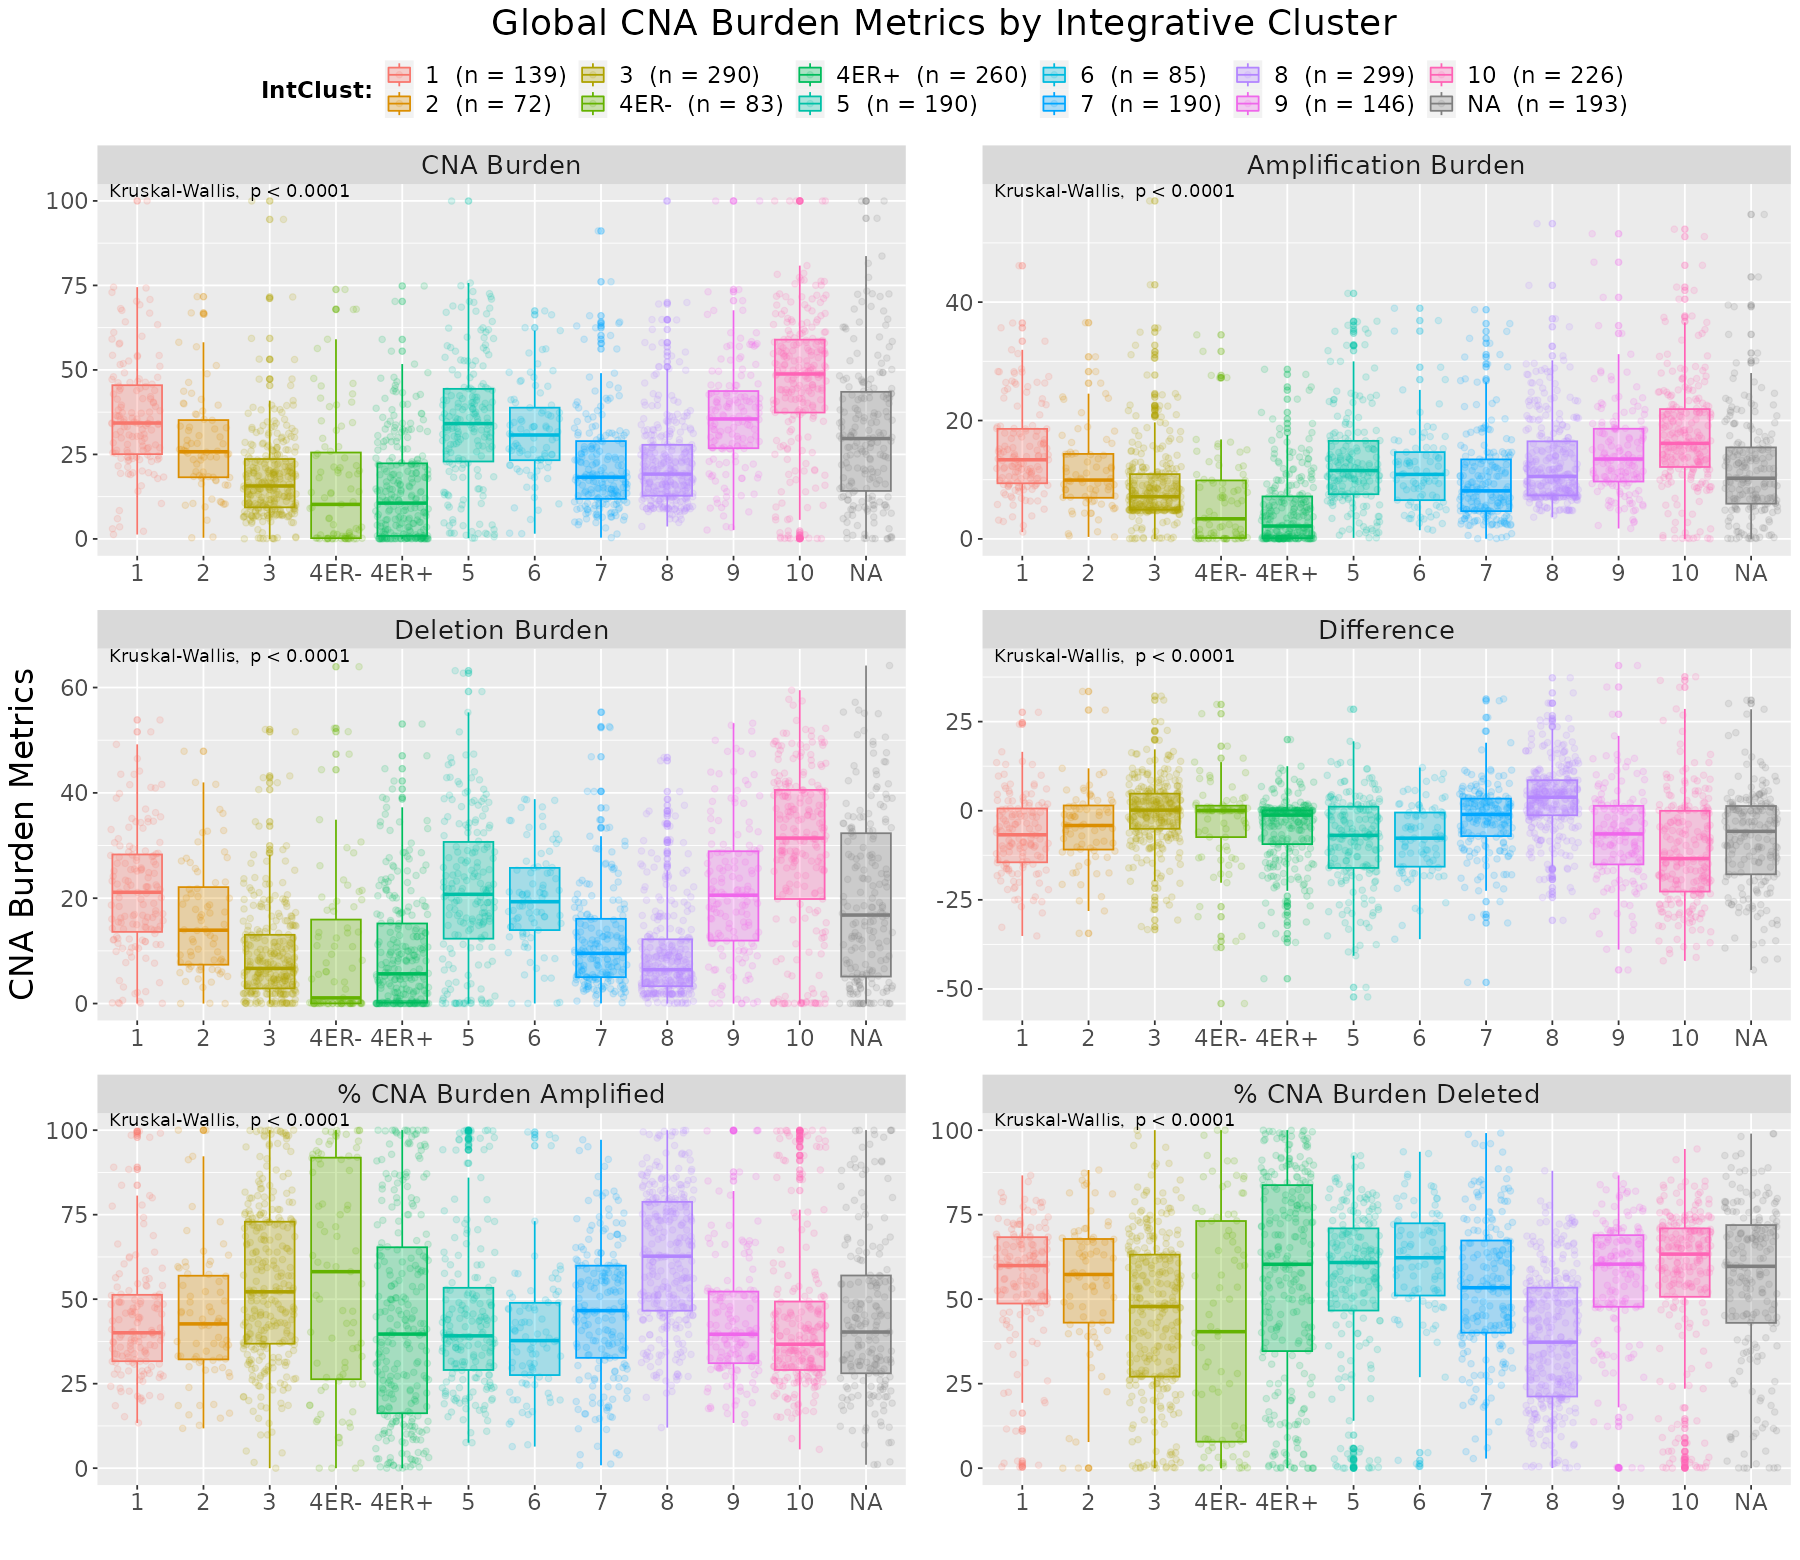
\includegraphics[width=1\textwidth]{../figures/Chapter_2/Global_CNA_Burden_Metrics_Across_IntClust.png}
\caption[Boxplots for each CNA Burden metric by Integrative Cluster.]{Boxplots for each CNA Burden metric by Integrative Cluster. Each facet contains boxplots for the CNA Burden metrics calculated using all available data and Benjamini-Hochberg adjusted Kruskal-Wallis p-values. NA denotes METABRIC patients missing Integrative Cluster information.}
\label{fig:CNA-Burden-Metric-Boxplots-IC}
\end{figure}

IntClust 10 displays the highest absolute, amplification and deletion CNA Score and Burden metrics (Dunn’s test $p < 0.0001$ for most comparisons, Tables \ref{tab:DT_Score_2} and \ref{tab:DT_Burden_2}). This is not surprising as IntClust 10 is primarily made up of Basal patients (Figure \ref{fig:Comp}). IntClust 1, 5 and 9 also display high levels of GI and are primarily composed of the PAM50 subtypes that have higher levels of GI, i.e. Basal, HER2 and Luminal B subtype. The densities of these distributions, apart from the CNA Amp metric distribution, are not significantly different from each other ($p > 0.05$). The levels of amplification burden observed in IntClust 5 are significantly lower than the levels observed in IntClust 1 and 9 ($p = 0.01$ and $p = 0.02$, respectively). IntClust 3, 4ER-, ER+, and 7 are primarily composed of Luminal A, Normal and Claudin-low subtypes (Figure \ref{fig:Comp}). These subtypes display low levels of GI and as such the boxplots display the lowest CNA Score and Burden metrics, except for CNA Del Score and Burden where IntClust 8 displays lower levels of deletions, when compared with IntClust 7. The distributions of IntClust 4ER- and 4ER+ do not significantly differ from each other, while IntClust 3 displays significantly more amplifications than IntClust 4ER+ and 4ER- ($p < 0.0001$ and $p < 0.01$, respectively), and IntClust 7 has significantly higher distributions across all metrics ($p < 0.01$, Tables \ref{tab:DT_Score_2} and \ref{tab:DT_Burden_2}).

Focusing on the direct comparison of levels of amplification to deletion within each IntClust, Figures \ref{fig:CNA-Score-Metric-Boxplots-IC-AmpDel} and \ref{fig:CNA-Burden-Metric-Boxplots-IC-AmpDel}, IntClust 2, 5 and 10, three clusters associated with poorer survival outcome, have significantly higher levels of deletions than amplifications ($p = 0.034$, $p < 0.0001$ and $p < 0.0001$, respectively). IntClust 1, 4ER+ and 6 also display significantly more deletions than amplifications but correspond to intermediate or good survival outcome ($p < 0.0001$, $p = 0.0005$ and $p < 0.0001$, respectively). The remaining IntClust classifications observed by \cite{pmid22522925} to have favourable survival outcomes, i.e. IntClust 3, 4ER-, 7 and 8, show no significant difference in the levels of amplifications and deletions, IntClust 3, 4ER-, 7 ($p > 0.05$) or significantly more amplifications than deletions, IntClust 8 ($p < 0.0001$).

\begin{table}[!ht]
\caption[Comparisons of CNA Score metric distributions by Integrative Cluster.]{Comparisons of CNA Score metric distributions by Integrative Cluster. Z statistics and Benjamini-Hochberg adjusted p-values for each Dunn's test are shown.}
\begin{minipage}[c]{0.45\textwidth}
\centering
\begin{tabular}{ccc}
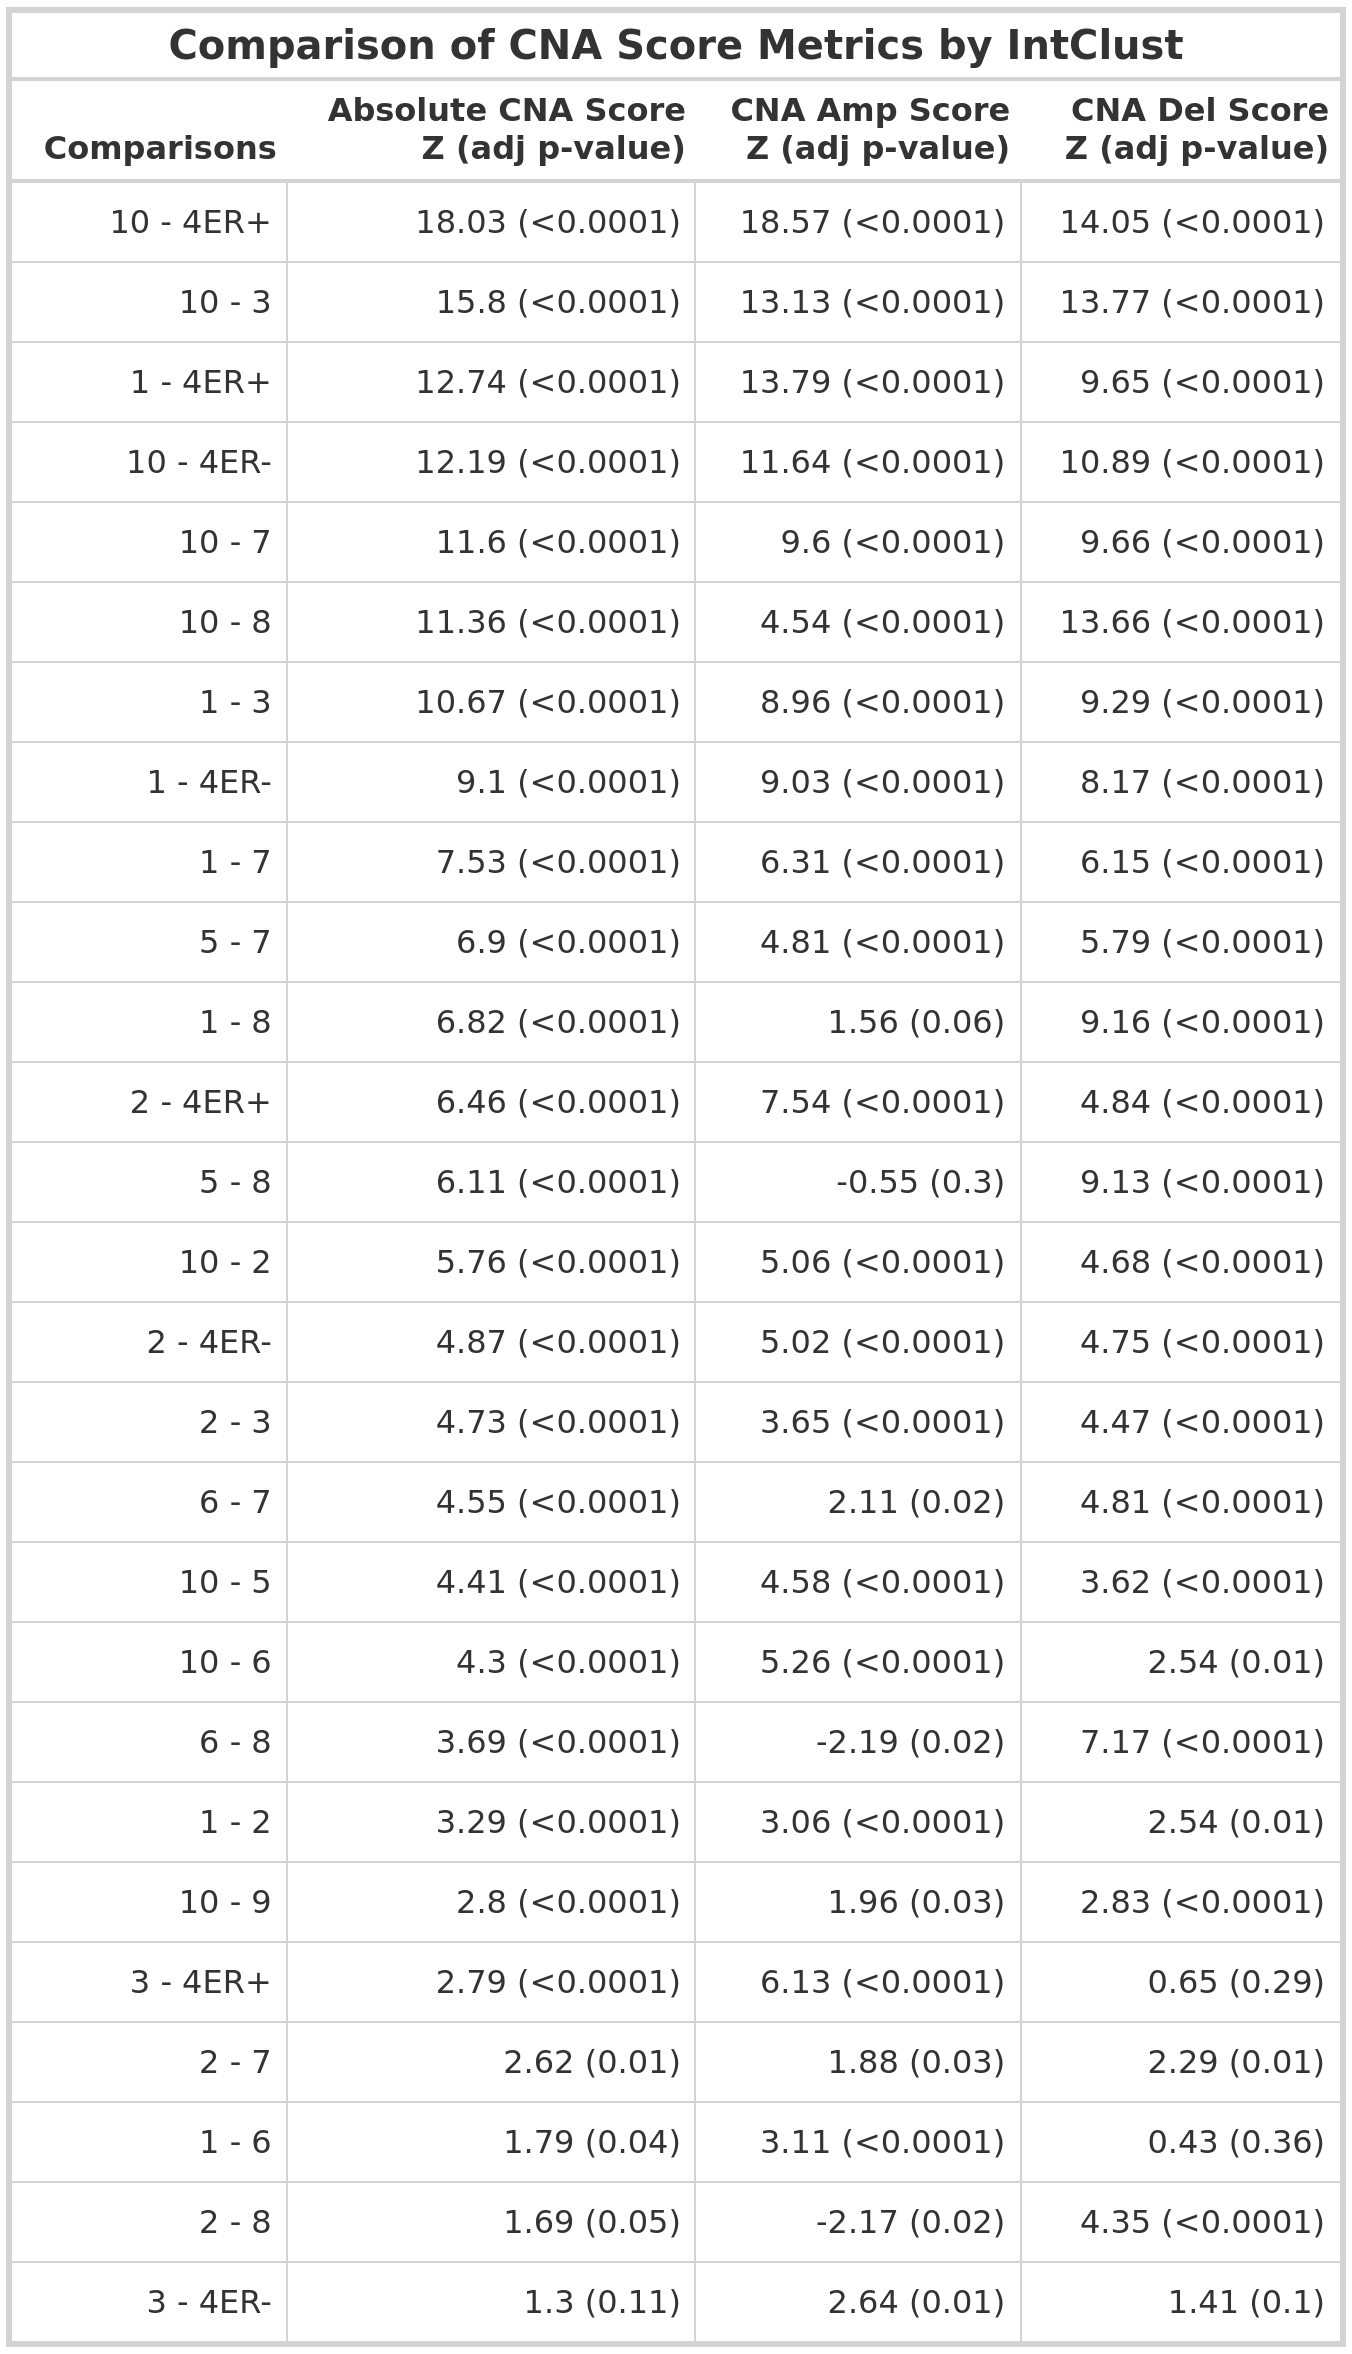
\includegraphics[width=0.98\textwidth]{../tables/Chapter_2/Global_CNA_Score_Metric_IntClust_Comparisons_1.png}
\end{tabular}
\end{minipage}
\hspace{0.8cm}
\begin{minipage}[c]{0.45\textwidth}
\centering
\begin{tabular}{ccc}
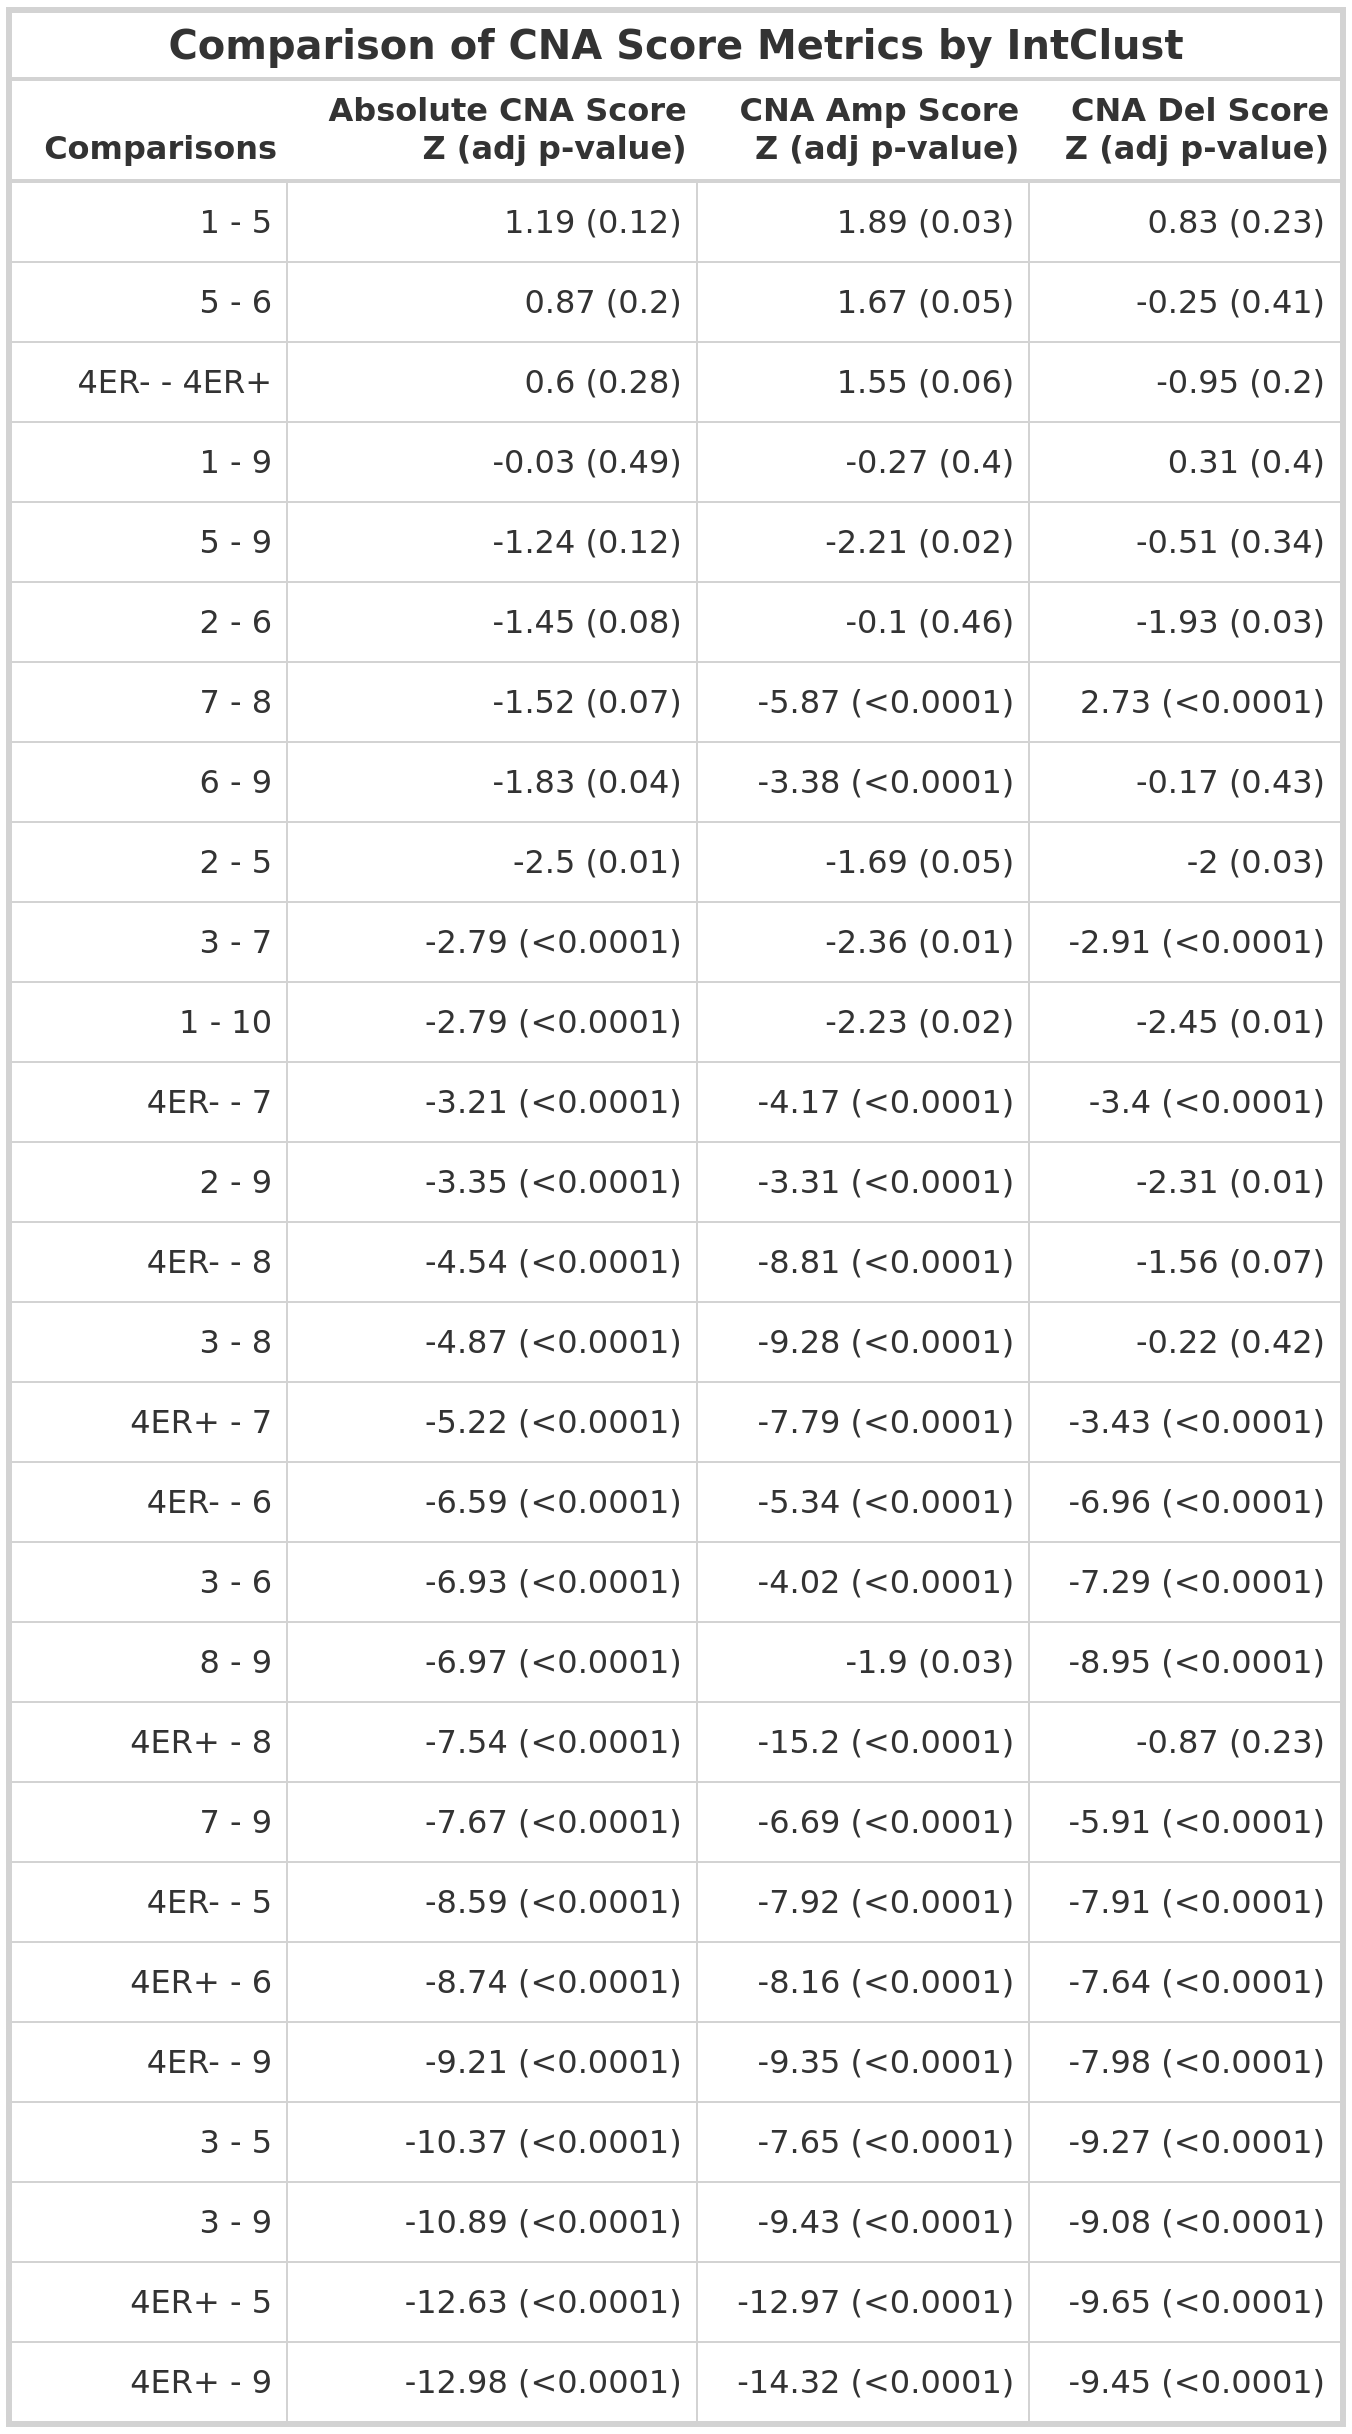
\includegraphics[width=0.96\textwidth]{../tables/Chapter_2/Global_CNA_Score_Metric_IntClust_Comparisons_2.png}
\end{tabular}
\end{minipage}
\label{tab:DT_Score_2}
\end{table}

\begin{figure}[!ht]
\center
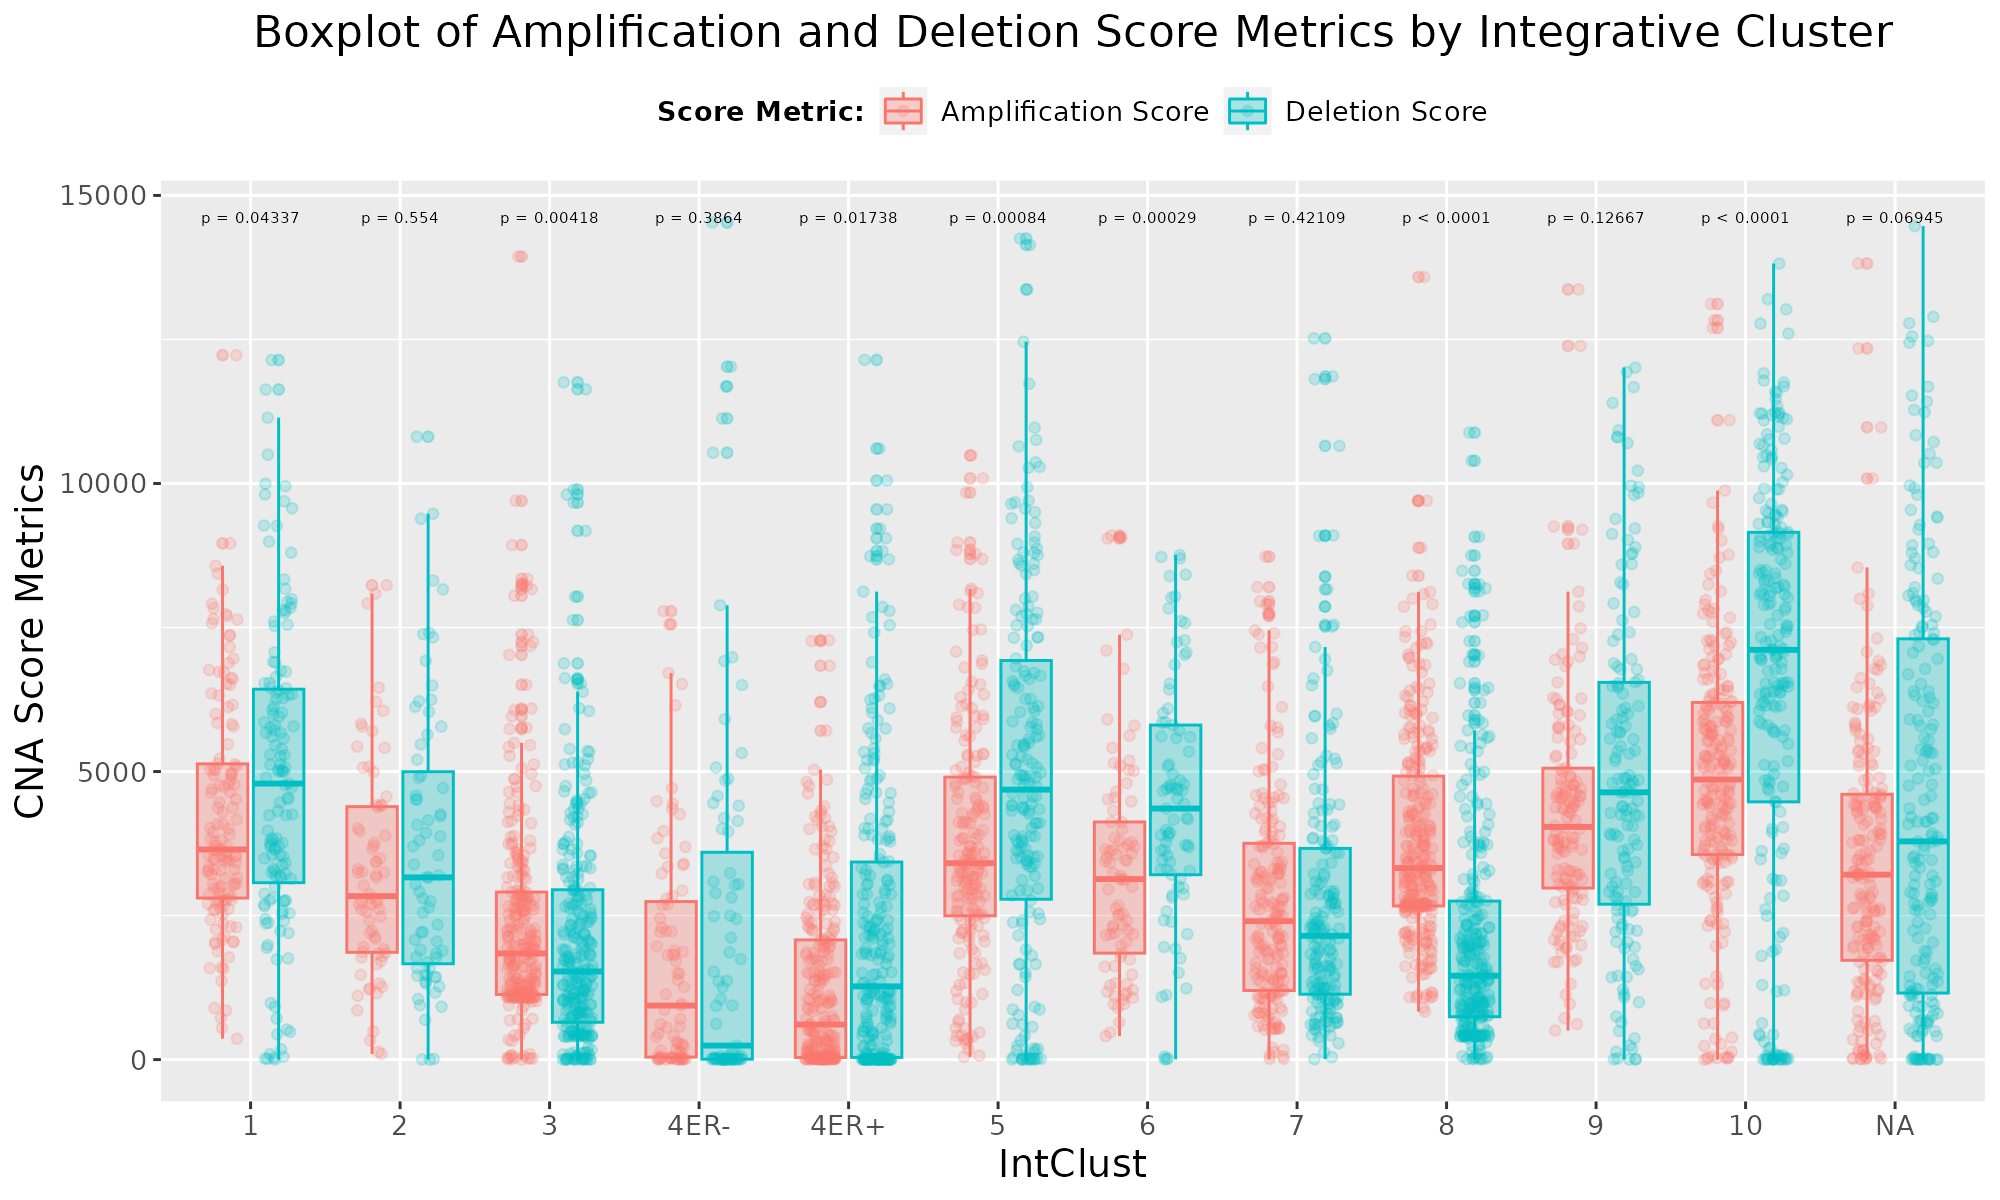
\includegraphics[width=0.97\textwidth]{../figures/Chapter_2/Global_CNA_Score_AmpDel_Across_IC.png}
\caption[Boxplots for each CNA Amp and CNA Del Score metric by Integrative Cluster.]{Boxplots for each CNA Amp and CNA Del Score metric by Integrative Cluster. Includes Benjamini-Hochberg adjusted Kruskal-Wallis p-values.}
\label{fig:CNA-Score-Metric-Boxplots-IC-AmpDel}
\end{figure}

\begin{table}[!ht]
\caption[Comparisons of CNA Burden metric distributions by Integrative Cluster.]{Comparisons of CNA Burden metric distributions by Integrative Cluster. Z statistics and Benjamini-Hochberg adjusted p-values for each Dunn's test are shown.}
\begin{minipage}[c]{0.45\textwidth}
\centering
\begin{tabular}{ccc}
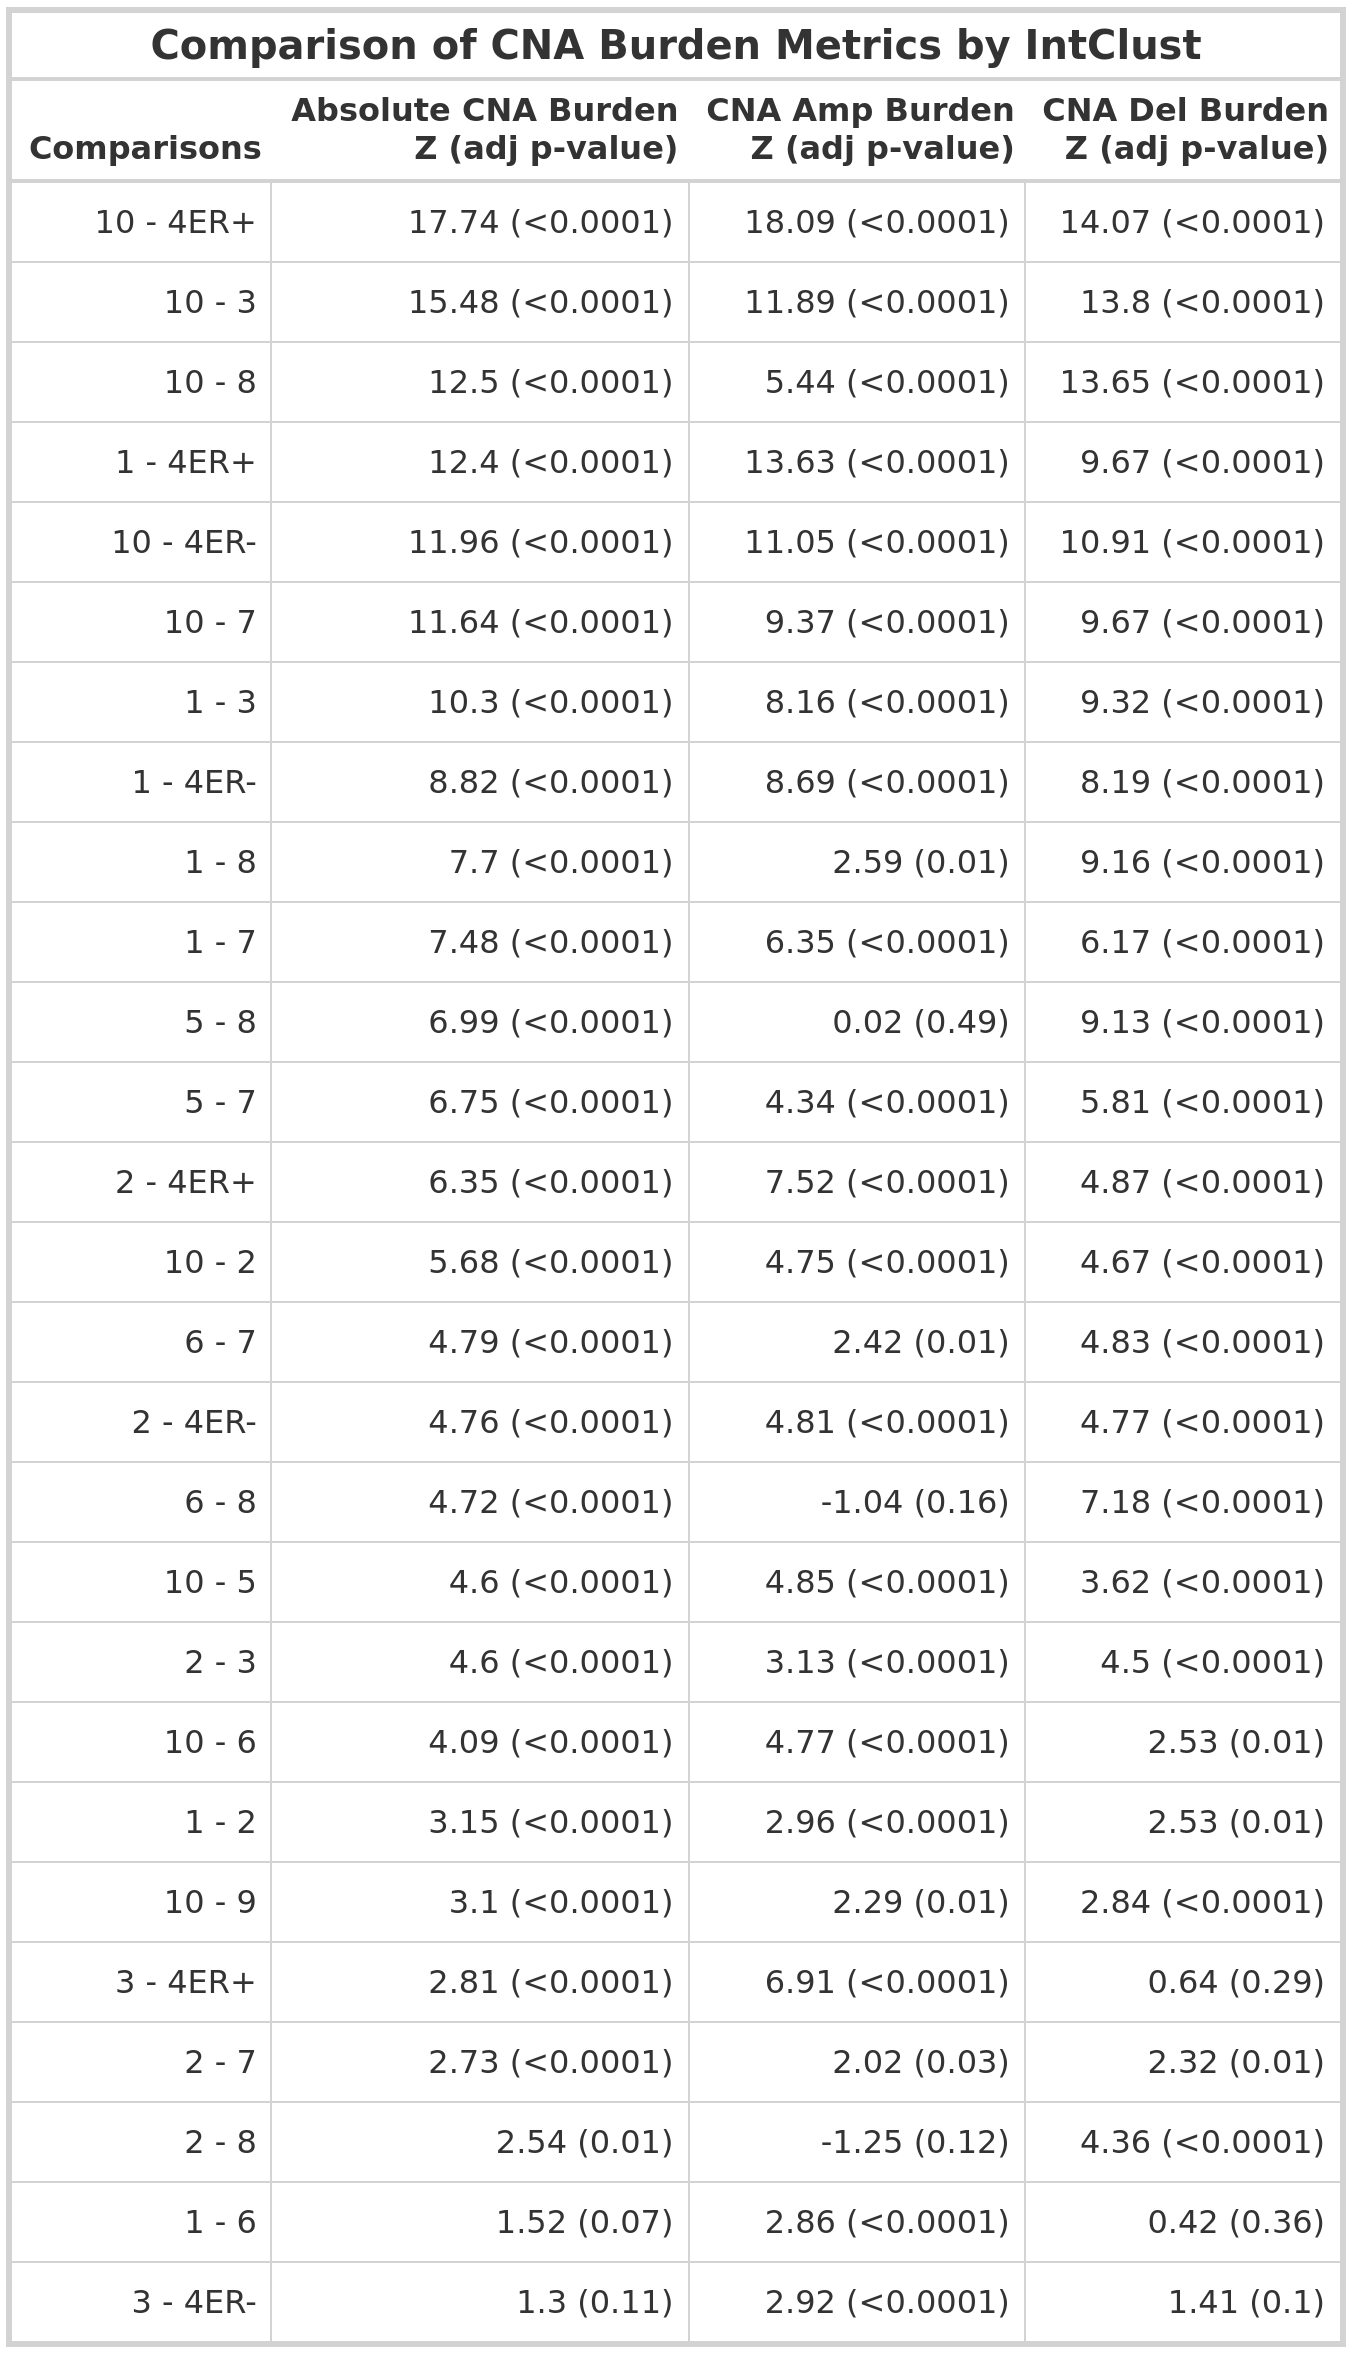
\includegraphics[width=0.98\textwidth]{../tables/Chapter_2/Global_CNA_Burden_Metric_IntClust_Comparisons_1.png}
\end{tabular}
\end{minipage}
\hspace{0.8cm}
\begin{minipage}[c]{0.45\textwidth}
\centering
\begin{tabular}{ccc}
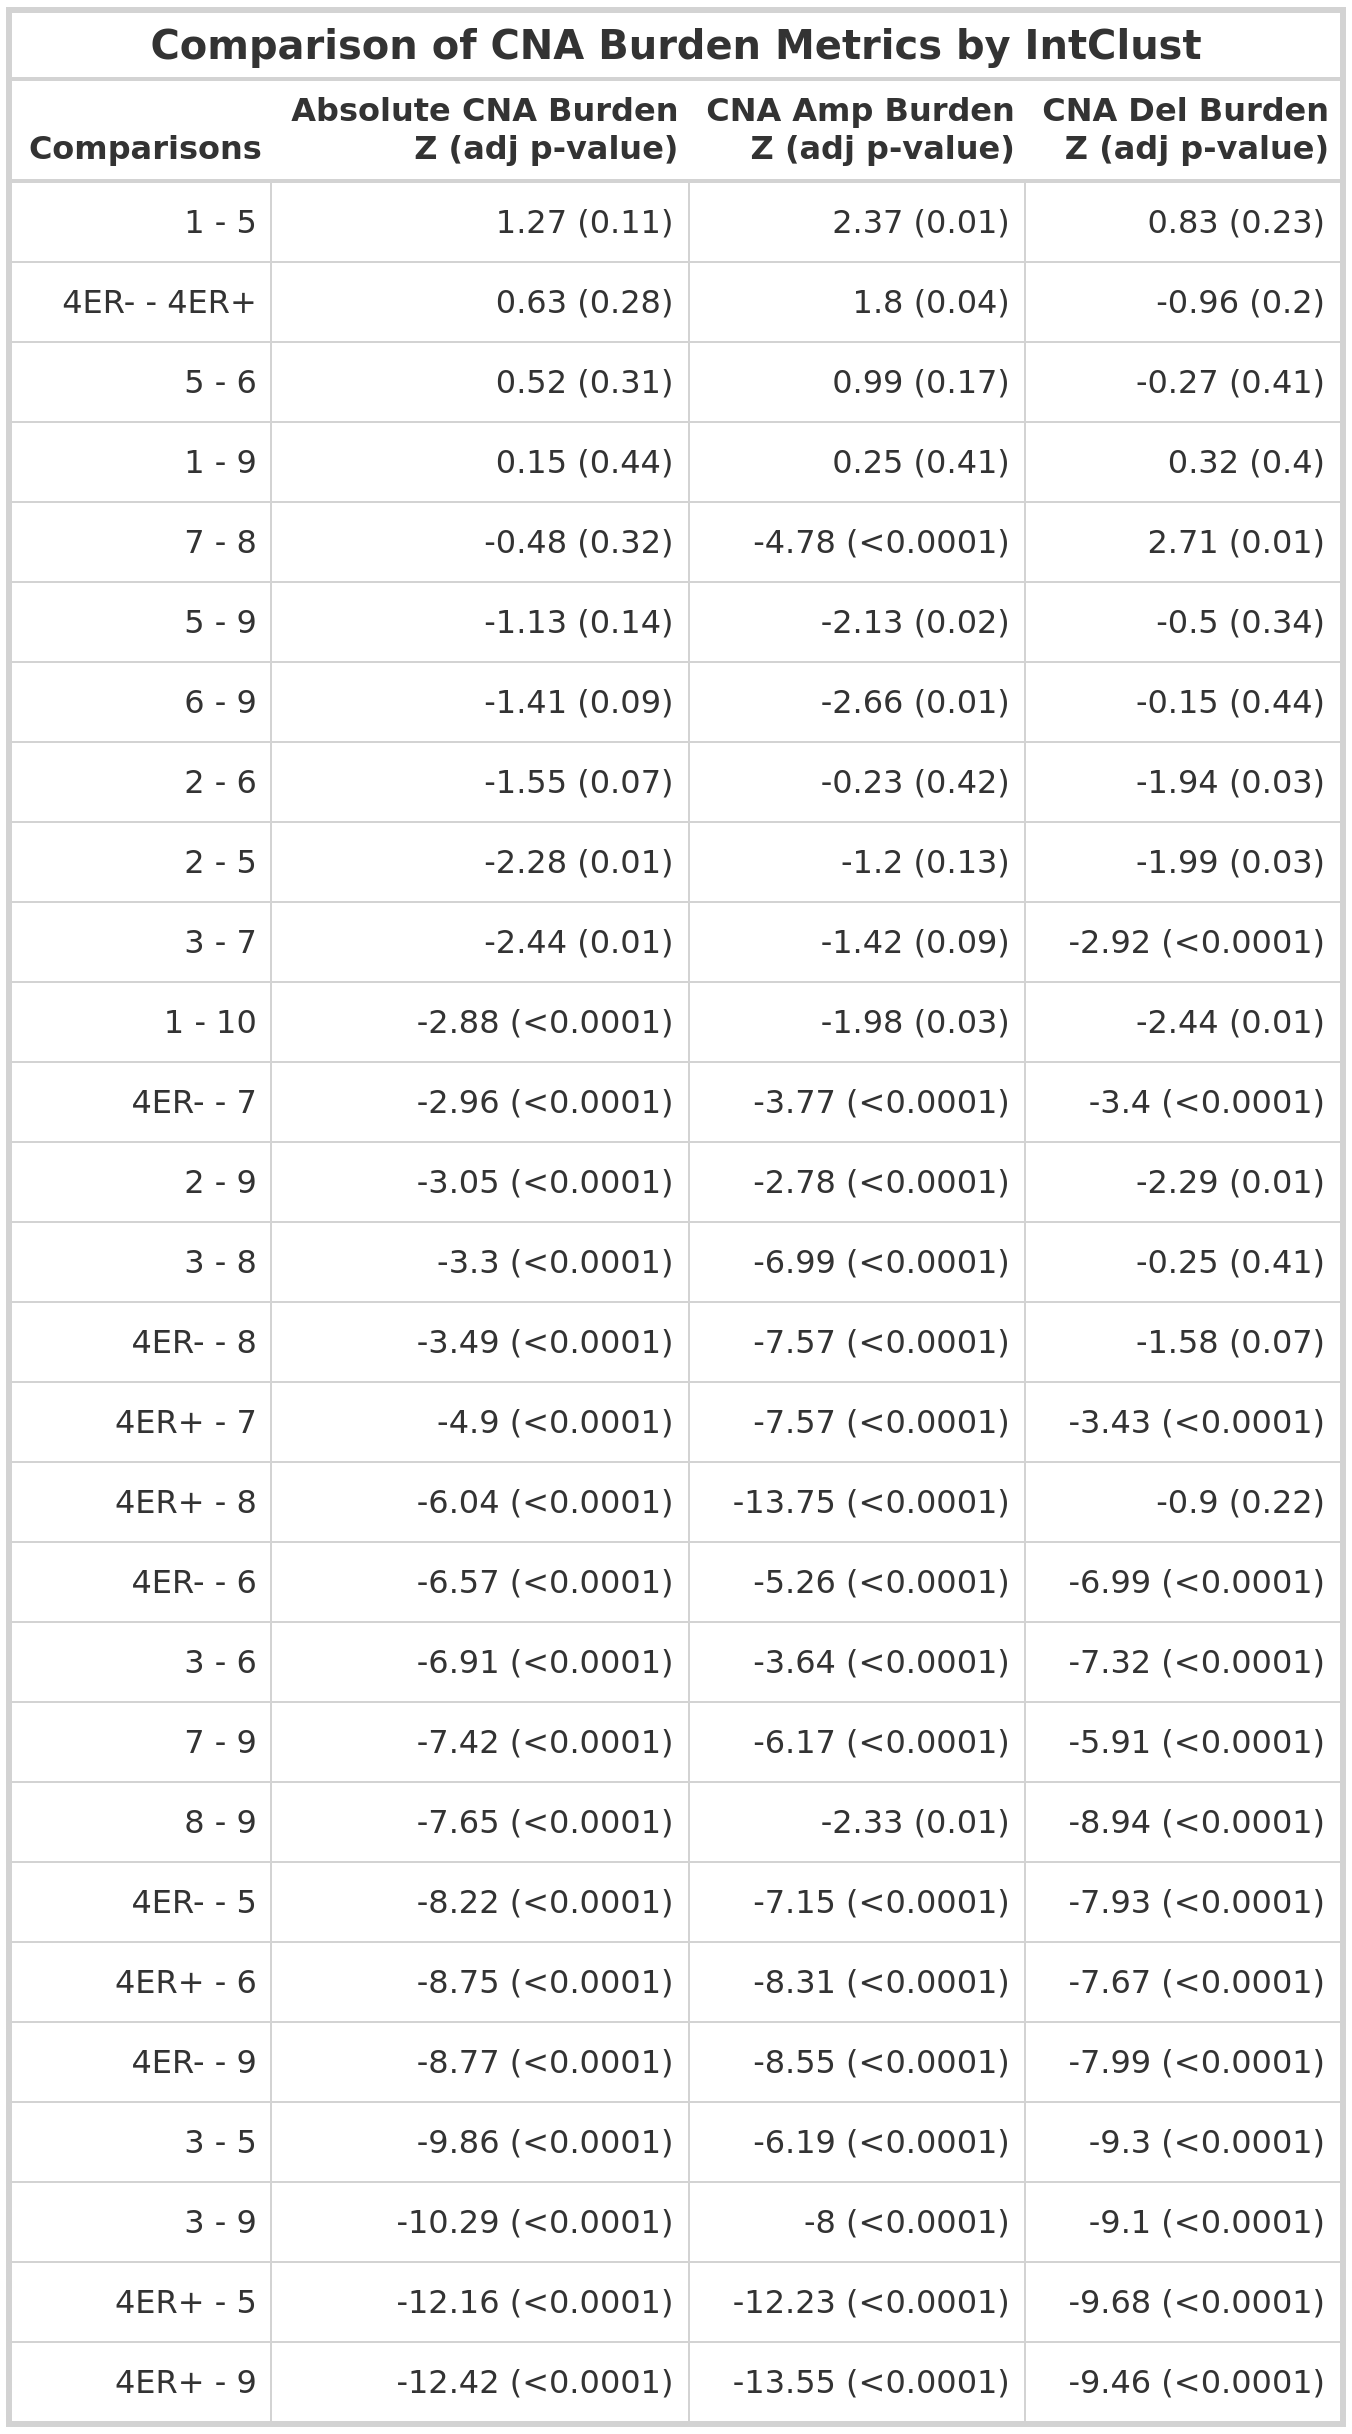
\includegraphics[width=0.96\textwidth]{../tables/Chapter_2/Global_CNA_Burden_Metric_IntClust_Comparisons_2.png}
\end{tabular}
\end{minipage}
\label{tab:DT_Burden_2}
\end{table}

\begin{figure}[!ht]
\center
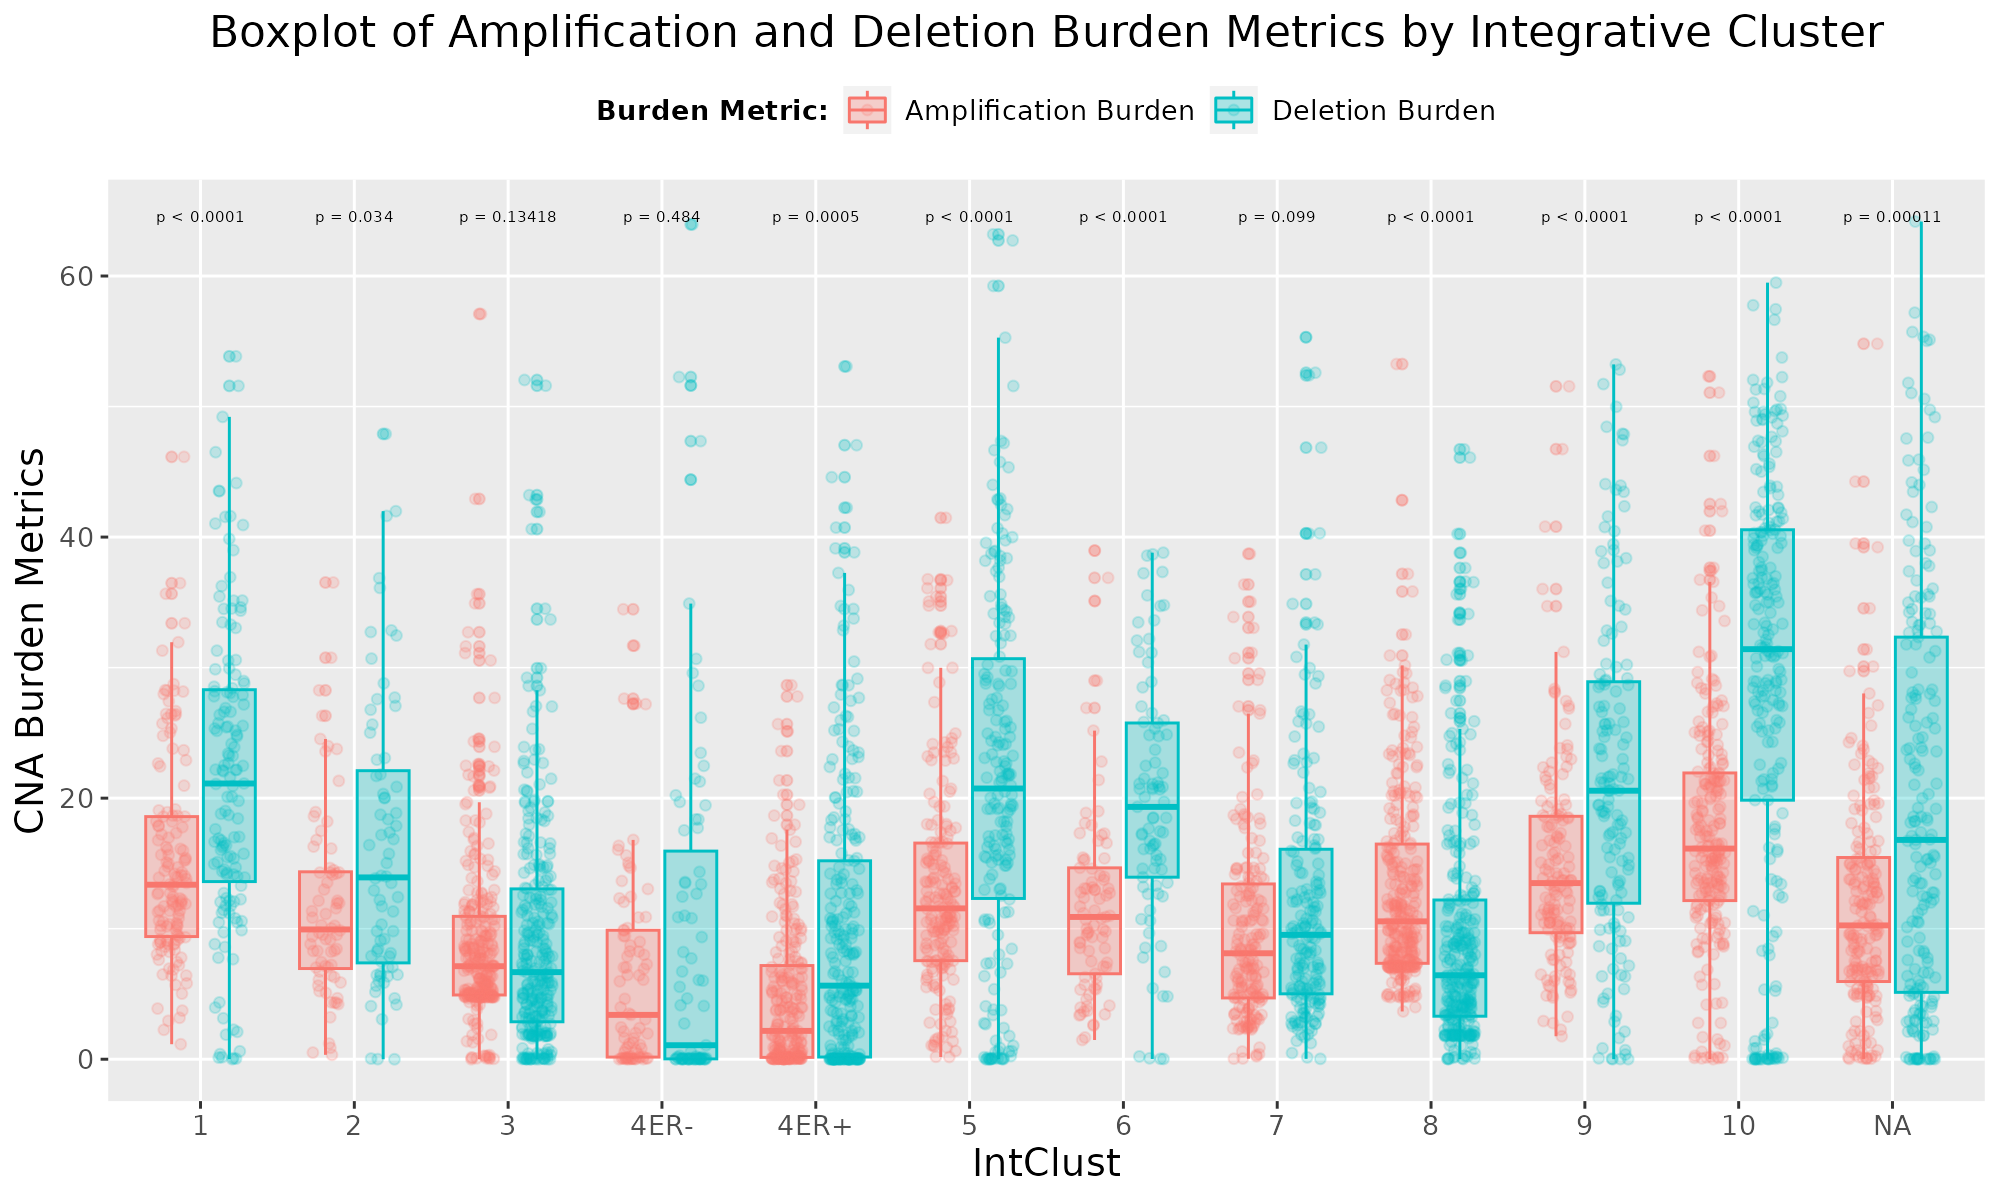
\includegraphics[width=0.97\textwidth]{../figures/Chapter_2/Global_CNA_Burden_AmpDel_Across_IC.png}
\caption[Boxplots for each CNA Amp and CNA Del Burden metric by Integrative Cluster.]{Boxplots for each CNA Amp and CNA Del Burden metric by Integrative Cluster. Includes Benjamini-Hochberg adjusted Kruskal-Wallis p-values.}
\label{fig:CNA-Burden-Metric-Boxplots-IC-AmpDel}
\end{figure}
\clearpage 

\subsubsection{Observed Distributions for Chromosome Arm CNA Metrics across Molecular Subtype Classifications}
\label{ObsDis1}
A similar association analysis is conducted for the 42 chromosome arm CNA Score and Burden metrics. In general, we observe similar effects comparing stratified subgroups of patients in the chromosome arm metrics as observed in the global metrics. 

Although Basal patients displayed widespread GI, some noteworthy alterations primarily observed in Basal patients include high levels of amplifications on chromosome 3q and 10p and deletions on chromosome 3p, 4p, 5q and 15q (Figure \ref{fig:PA-CNA-Score-Metric-Density-P50-5q}). Figure \ref{fig:PA-CNA-Score-Metric-Density-P50-5q} indicates that some significant difference exists comparing each of the selected CNA Burden metric distributions across PAM50 subtype ($p<0.0001$). Applying Dunn's Test to each CNA Burden metric indicates Basal patients display the highest CNA Burden metric across all subtypes, with $p<0.0001$ for all selected CNA metrics and comparisons, indicating higher levels of GI on the specified chromosome arms when compared to other PAM50 subtypes (Table \ref{tab:PA-CNA-Score-Metric-Density-P50-5q}). The highlighted chromosome arms correspond largely to those frequently altered in tumours displaying the “complex I” pattern, which are usually Basal tumours, observed in \cite{pmid17142309}.

Noteworthy alterations observed in HER2 patients include high levels of amplification on chromosome 1q, 8q and 17q, where the HER2 gene is located, and high levels of deletions on chromosome 8p, 17p and 17q (Figure \ref{fig:PA-CNA-Score-Metric-Density-P50-17q}). For each selected CNA Burden metric some significant difference exists comparing each of the CNA metric distributions across PAM50 subtype ($p<0.0001$). Performing pairwise comparisons indicates that HER2 patients display higher CNA Burden metric across the majority of selected CNA Burden metrics and PAM50 subtypes ($p<0.0001$) except when comparing to Basal patients (Table \ref{tab:PA-CNA-Score-Metric-Density-P50-5q} and \ref{tab:PA-CNA-Score-Metric-Density-P50-17q}). The distributions of the selected CNA Burden metrics in the HER2 and Basal subtypes do not significantly differ from each other ($p>0.05$) indicating similar levels of GI. Exceptions include CNA Amp Burden on chromosome 1q and CNA Amp Burden on chromosome 17q, where HER2 patients display lower and higher levels of amplifications, respectively, when compared with Basal patients ($p = 0.04$ and  $p<0.0001$). Interestingly high levels of deletions are also observed on chromosome 17q in HER2 patients, indicating amplification of HER2 locus may be correlated with widespread chromosome arm instability. 

For the Luminal patients, high levels of GI are documented on chromosome 1q and 16p (amplifications) and chromosome 16q (deletions) (Figures \ref{fig:PA-CNA-Score-Metric-Density-P50-17q} and \ref{fig:PA-CNA-Score-Metric-Density-P50-16q}). Luminal B patients display higher levels of whole genome instability than Luminal A patients (Tables \ref{tab:PA-CNA-Score-Metric-Density-P50-5q}-\ref{tab:PA-CNA-Score-Metric-Density-P50-16q}). In particular, Luminal B patients display significantly more amplifications on chromosome 8q and 17q (Table \ref{tab:PA-CNA-Score-Metric-Density-P50-17q}) and deletions on chromosome 11q and 13q ($p < 0.0001$, Table \ref{tab:PA-CNA-Score-Metric-Density-P50-16q}). Luminal A patients display more amplifications on chromosome 16p, and more deletions on chromosome 16q than Luminal B patients ($p<0.001$, Table \ref{tab:PA-CNA-Score-Metric-Density-P50-16q}). 

Some alterations consistently observed across the PAM50 subtypes associated with poorer survival, i.e. Basal, HER2 and Luminal B, include high levels of amplification on chromosome 8q and 17q and high levels of deletions on chromosome 8p, 13q and 17p. 

The observed patterns of instability, measured by our CNA Score and Burden metrics, within the IntClusts largely matched with what \cite{pmid22522925} documented previously. Other chromosome arms to note include, 3p and 4p, which display high levels of deletions for IntClust 10, and IntClust 5 and 10, respectively (Figure \ref{fig:PA_IC} and Table \ref{tab:PA_IC}). 

Overall, patients exhibiting the highest levels of GI across most of the chromosome arms correspond to the PAM50 and IntClusts associated with reduced survival. This is consistent with findings in the previous section, where patients with higher measures of GI generally have reduced survival.

\vfill
\begin{figure}[!h]
\center
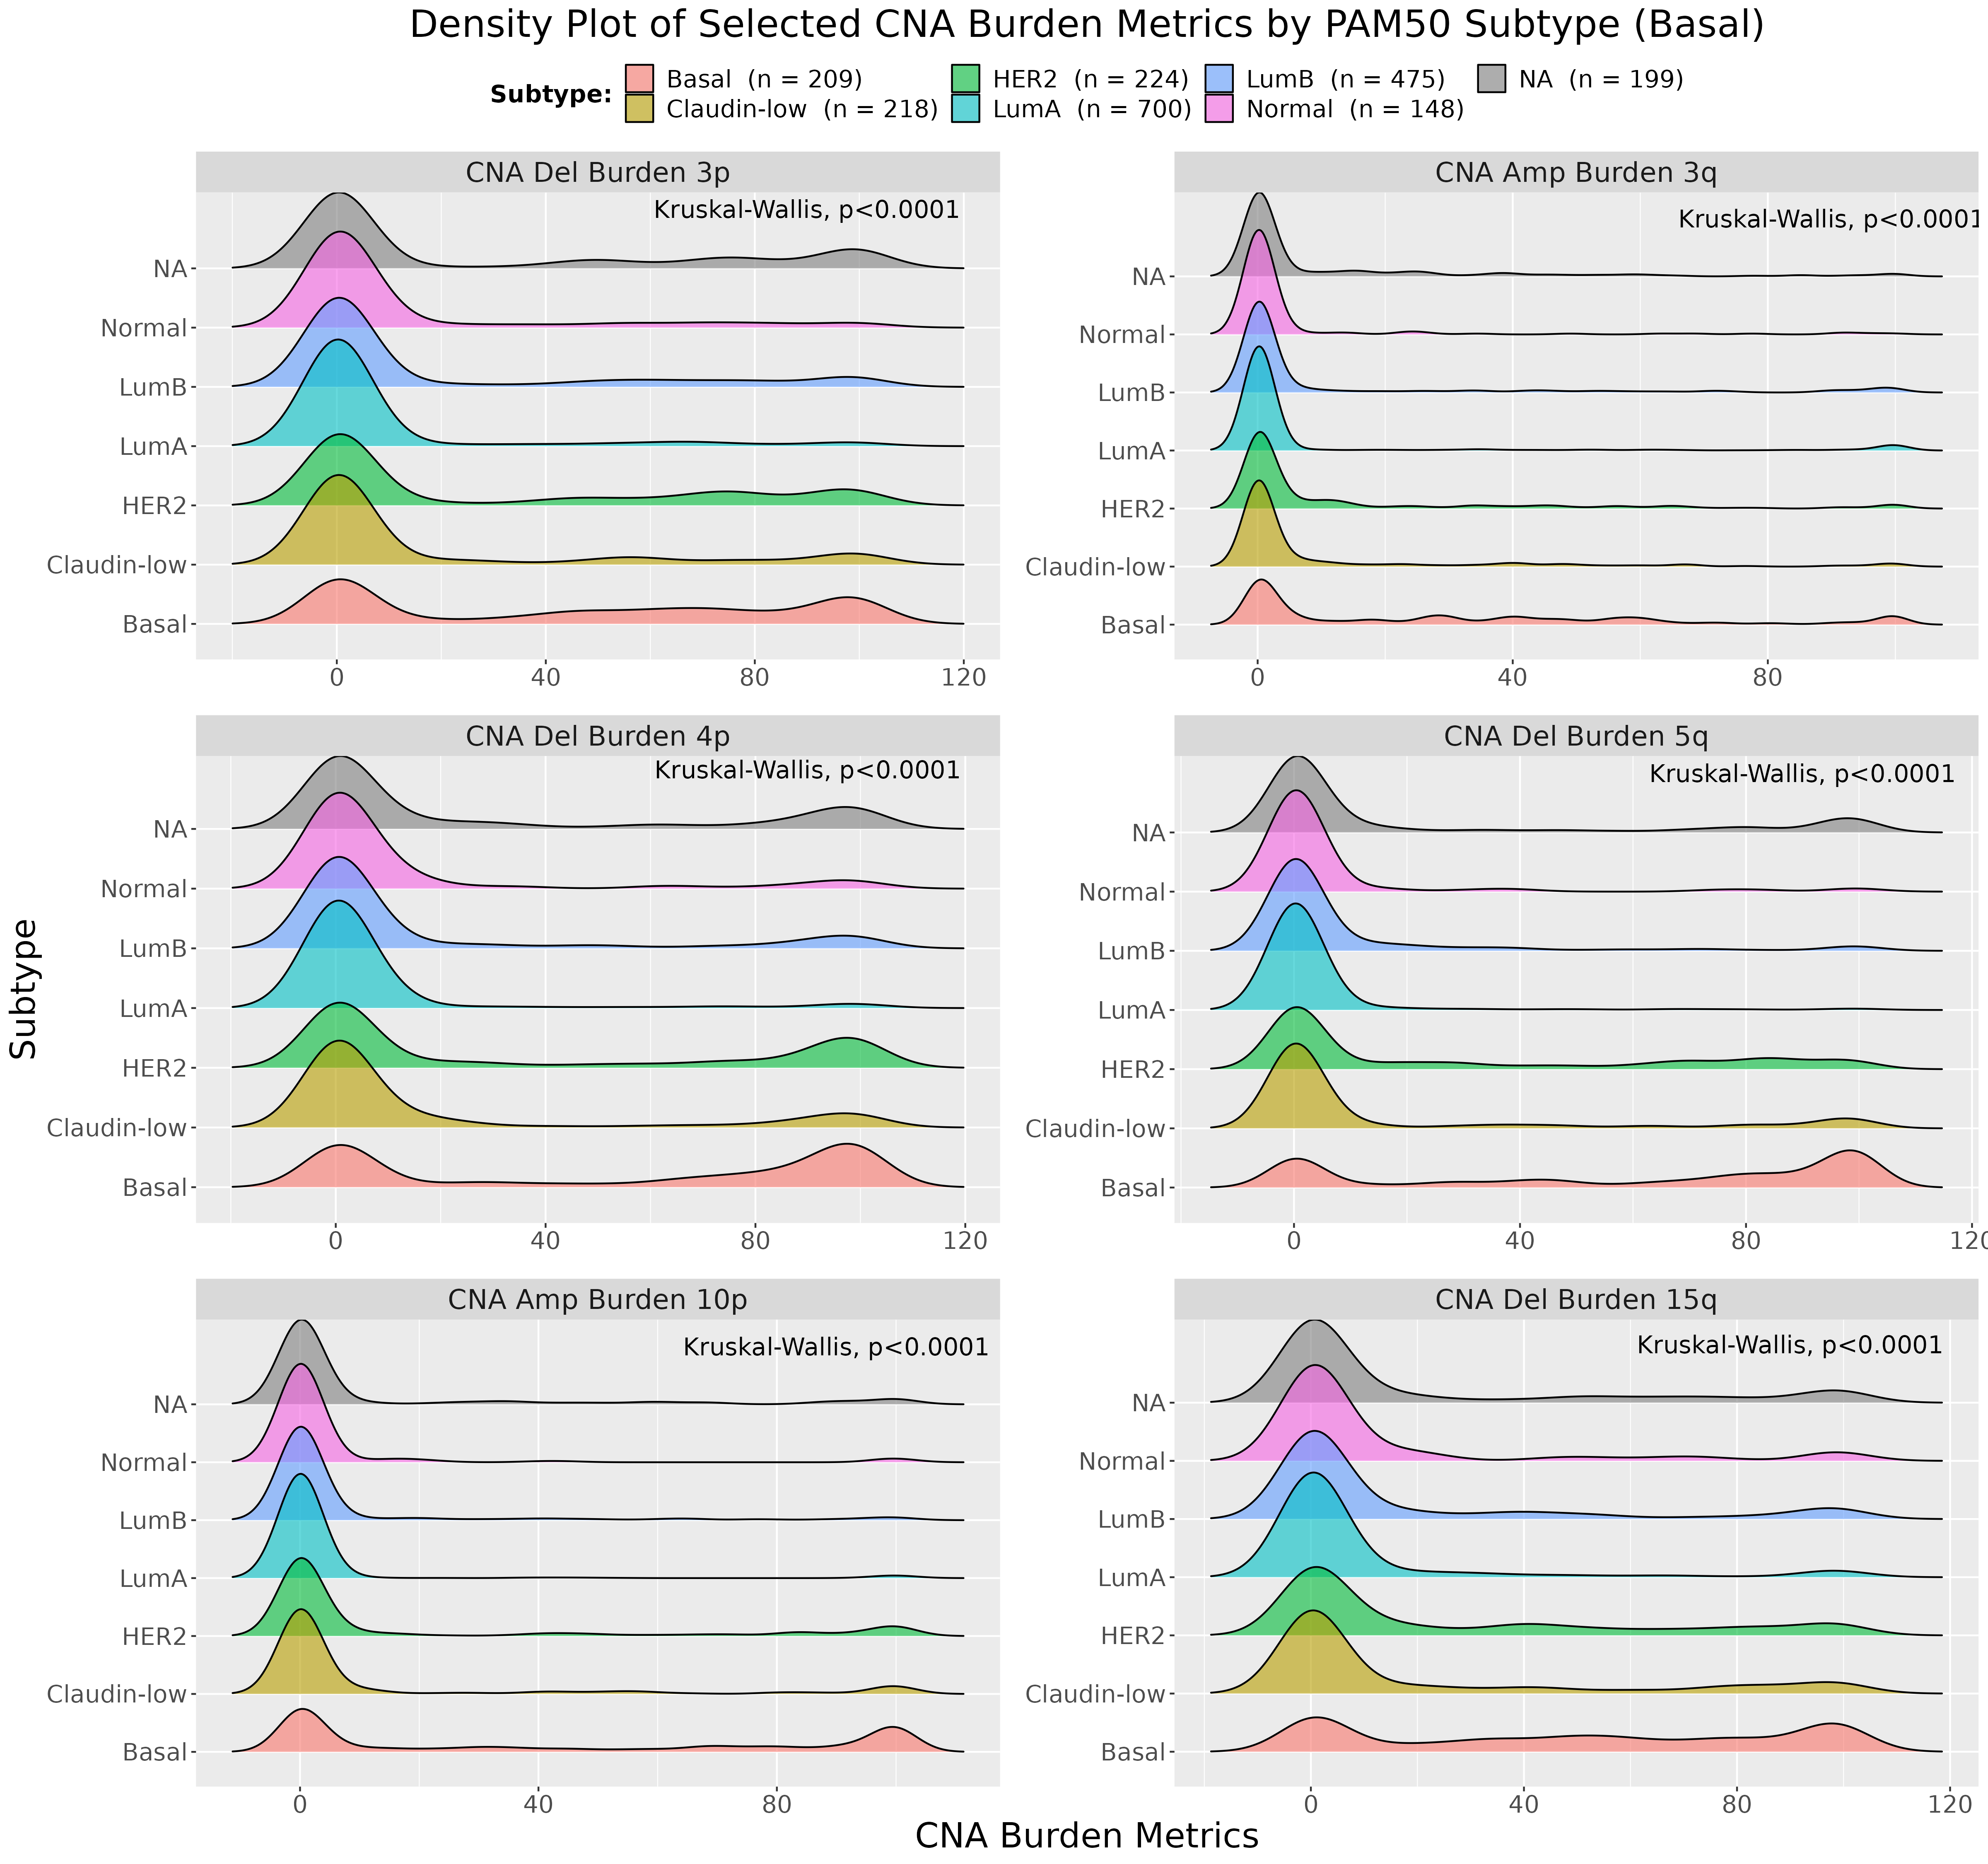
\includegraphics[width=1\textwidth]{../figures/Chapter_2/ChrArm_CNA_Burden_Metrics_Across_PAM50_Basal_Burden.png}
\caption[Density plots for each selected chromosome arm CNA Burden metric, with a focus on the Basal subtype.]{Density plots for each selected chromosome arm CNA Burden metric, with a focus on the Basal subtype. Chromosome arms where Basal patients display high GI are selected. Each facet contains boxplots for the chromosome arm CNA Burden metrics calculated using all available data and Benjamini-Hochberg adjusted Kruskal-Wallis p-values.}
\label{fig:PA-CNA-Score-Metric-Density-P50-5q}
\end{figure}
\vfill

\begin{table}[!htb]
\center
\caption[Comparisons of selected chromosome arm CNA Burden metric distributions by PAM50 subtype, with a focus on the Basal subtype.]{Comparisons of selected chromosome arm CNA Burden metric distributions by PAM50 subtype, with a focus on the Basal subtype. Chromosome arms where Basal patients display high GI are selected. Z statistics and Benjamini-Hochberg adjusted p-values are shown.}
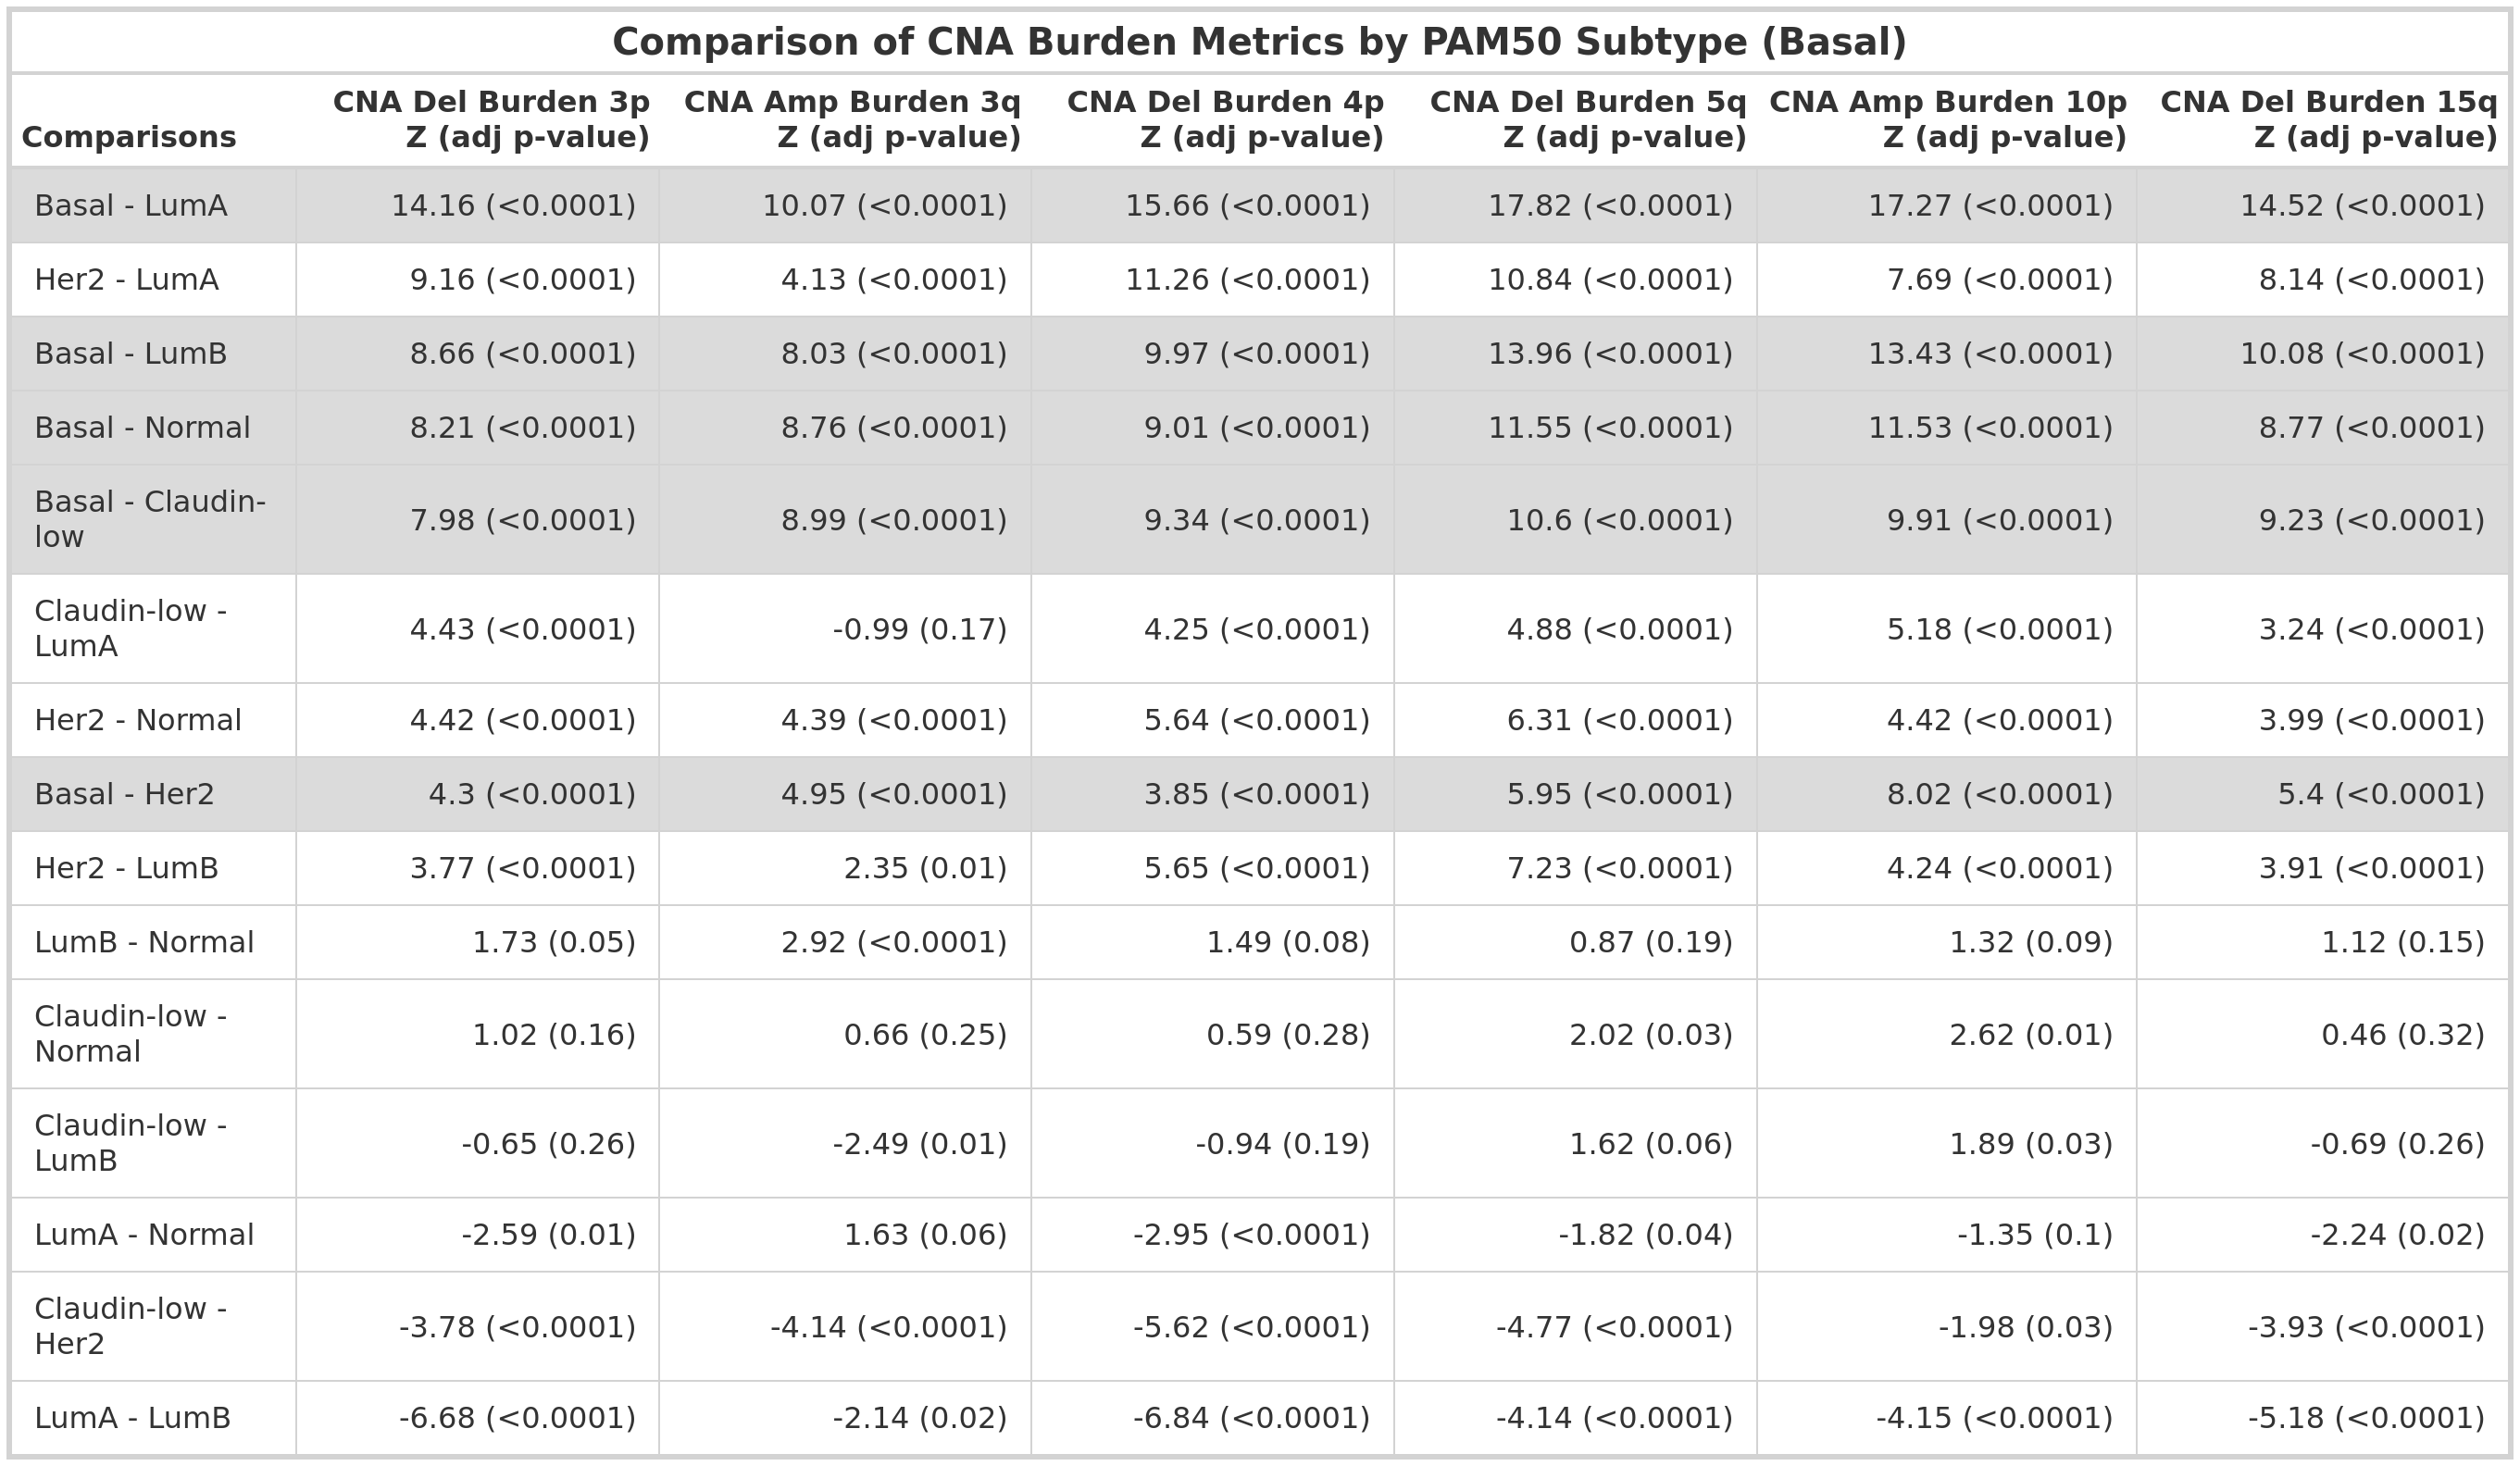
\includegraphics[width=1\textwidth]{../tables/Chapter_2/ChrArm_CNA_Burden_Metric_Comparisons_Basal.png}
\label{tab:PA-CNA-Score-Metric-Density-P50-5q}
\end{table}

\begin{figure}[!ht]
\center
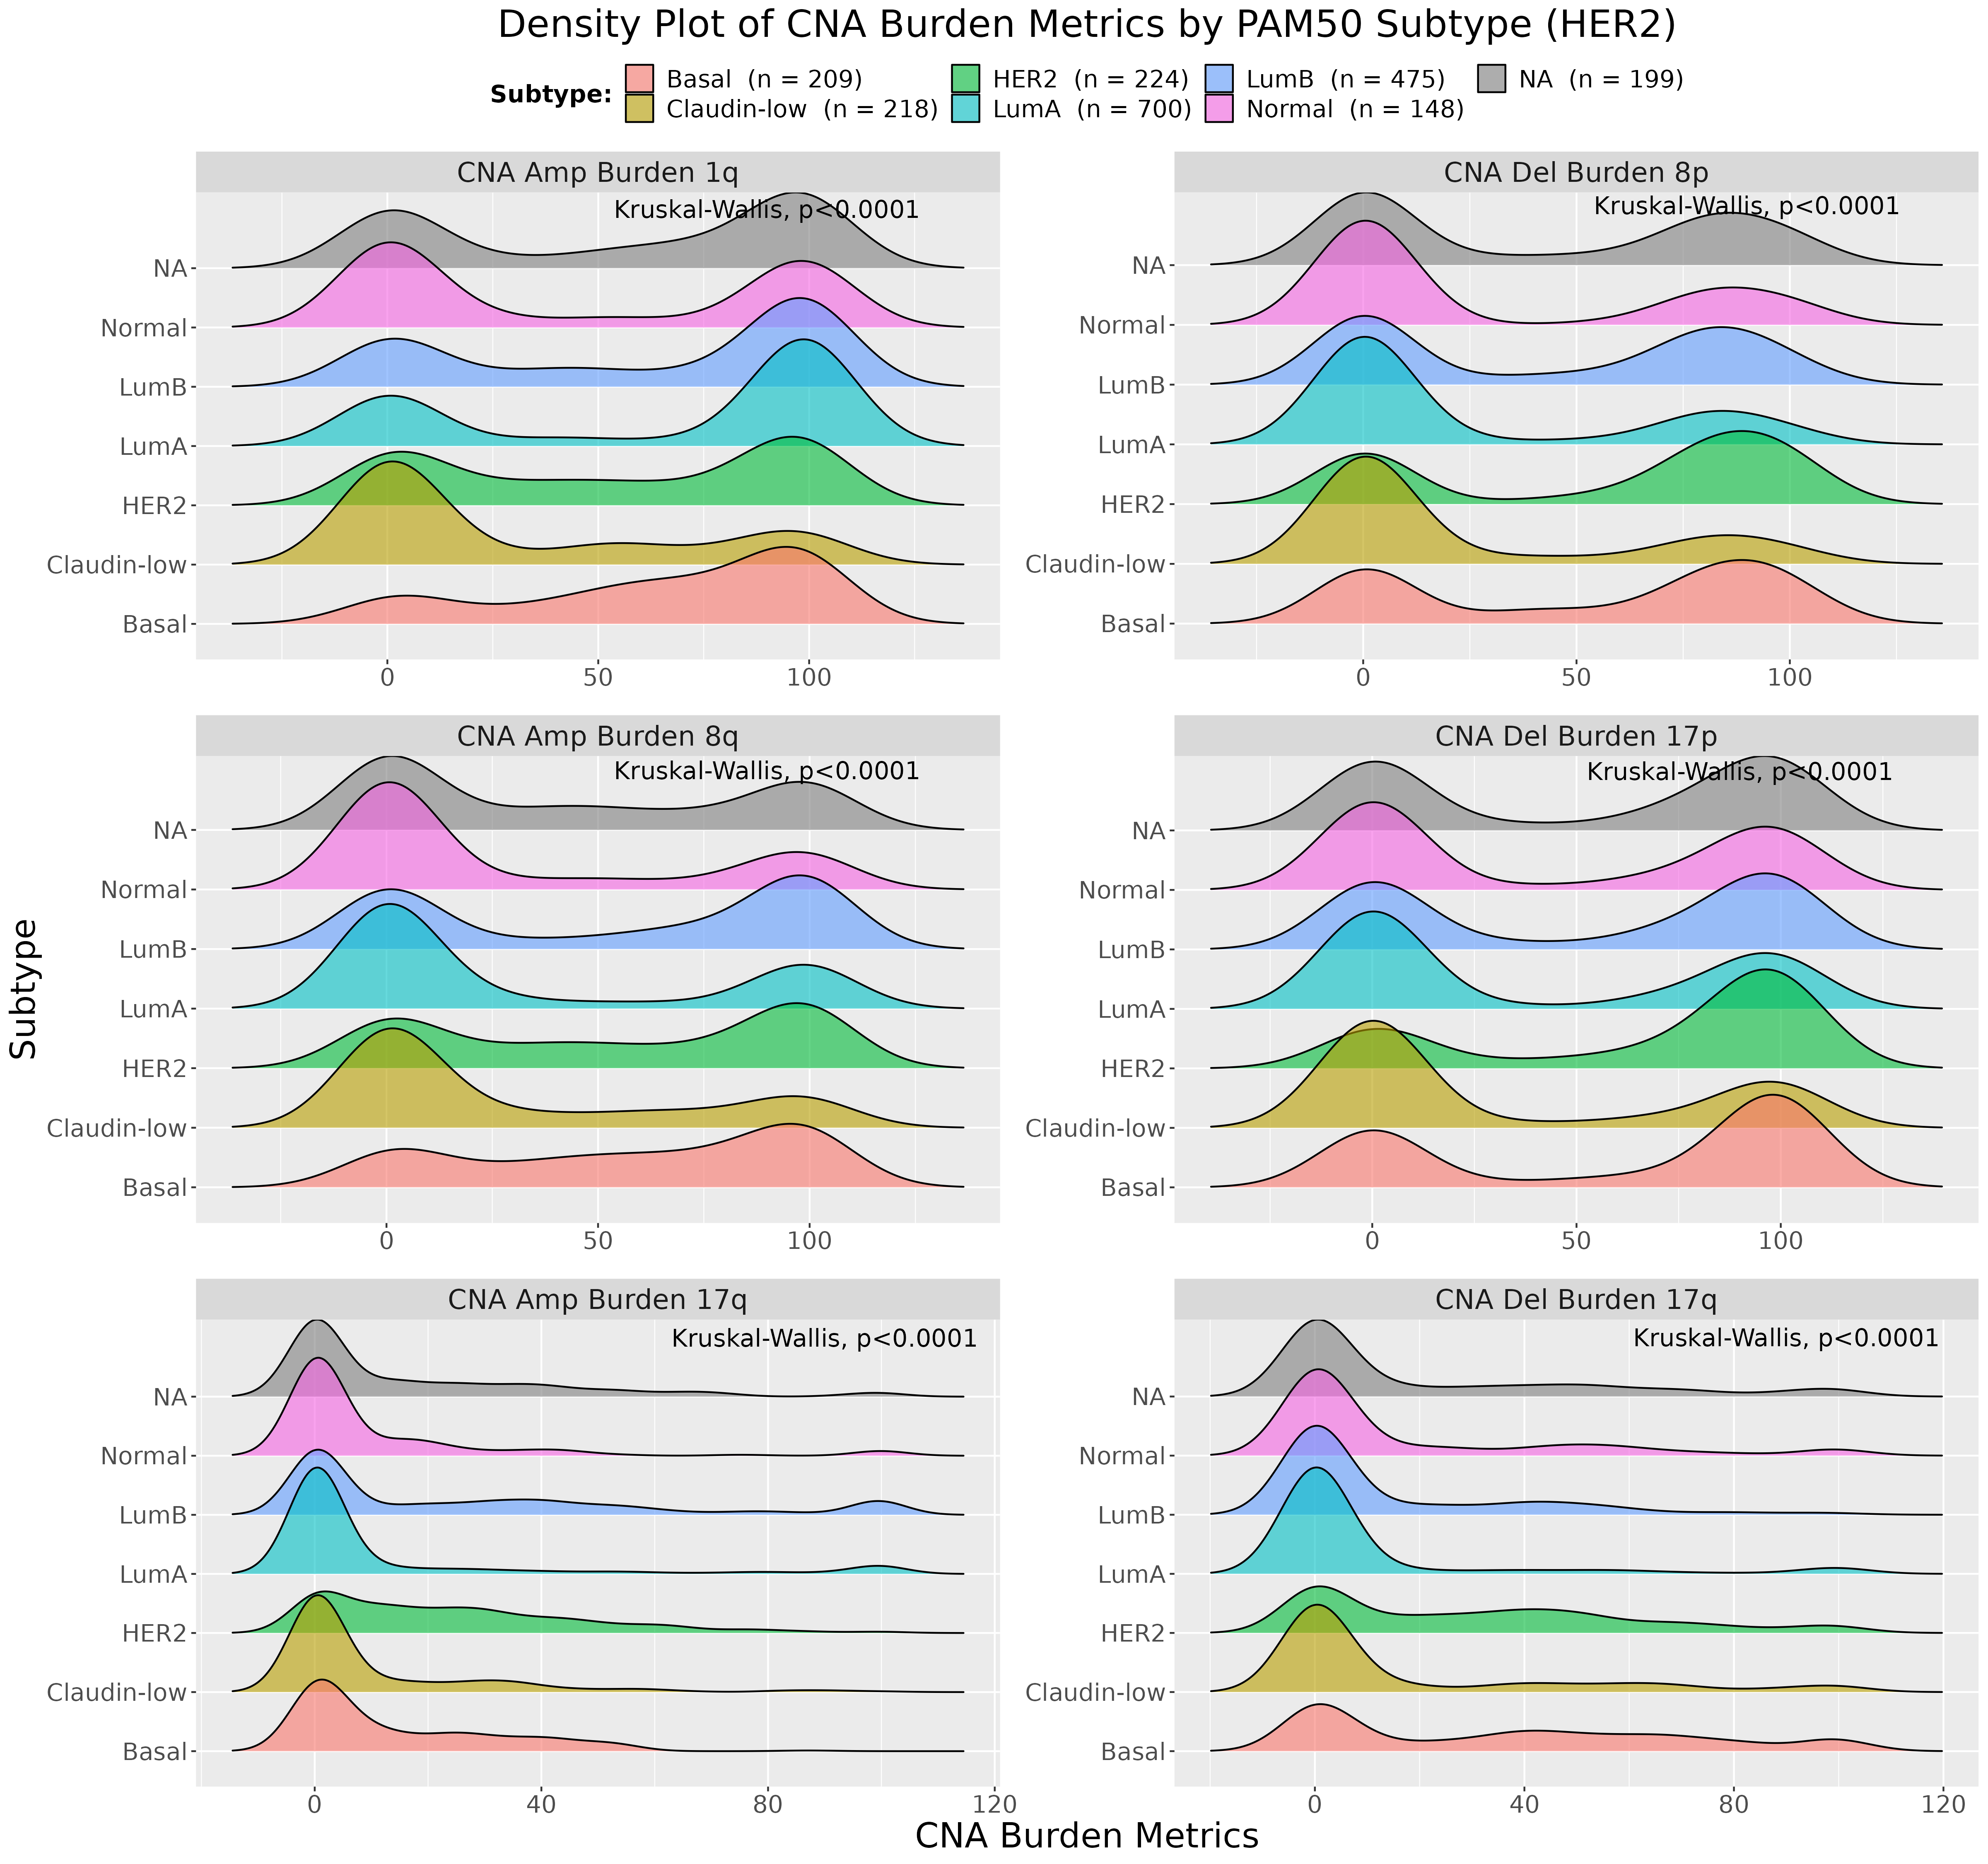
\includegraphics[width=1\textwidth]{../figures/Chapter_2/ChrArm_CNA_Burden_Metrics_Across_PAM50_HER2_Burden.png}
\caption[Density plots for each selected chromosome arm CNA Burden metric, with a focus on the HER2 subtype.]{Density plots for each selected chromosome arm CNA Burden metric, with a focus on the HER2 subtype. Chromosome arms where HER2 patients display high GI are selected. Each facet contains boxplots for the chromosome arm CNA Burden metrics calculated using all available data and Benjamini-Hochberg adjusted Kruskal-Wallis p-values.}

\label{fig:PA-CNA-Score-Metric-Density-P50-17q}
\end{figure}

\begin{figure}[!htb]
\center
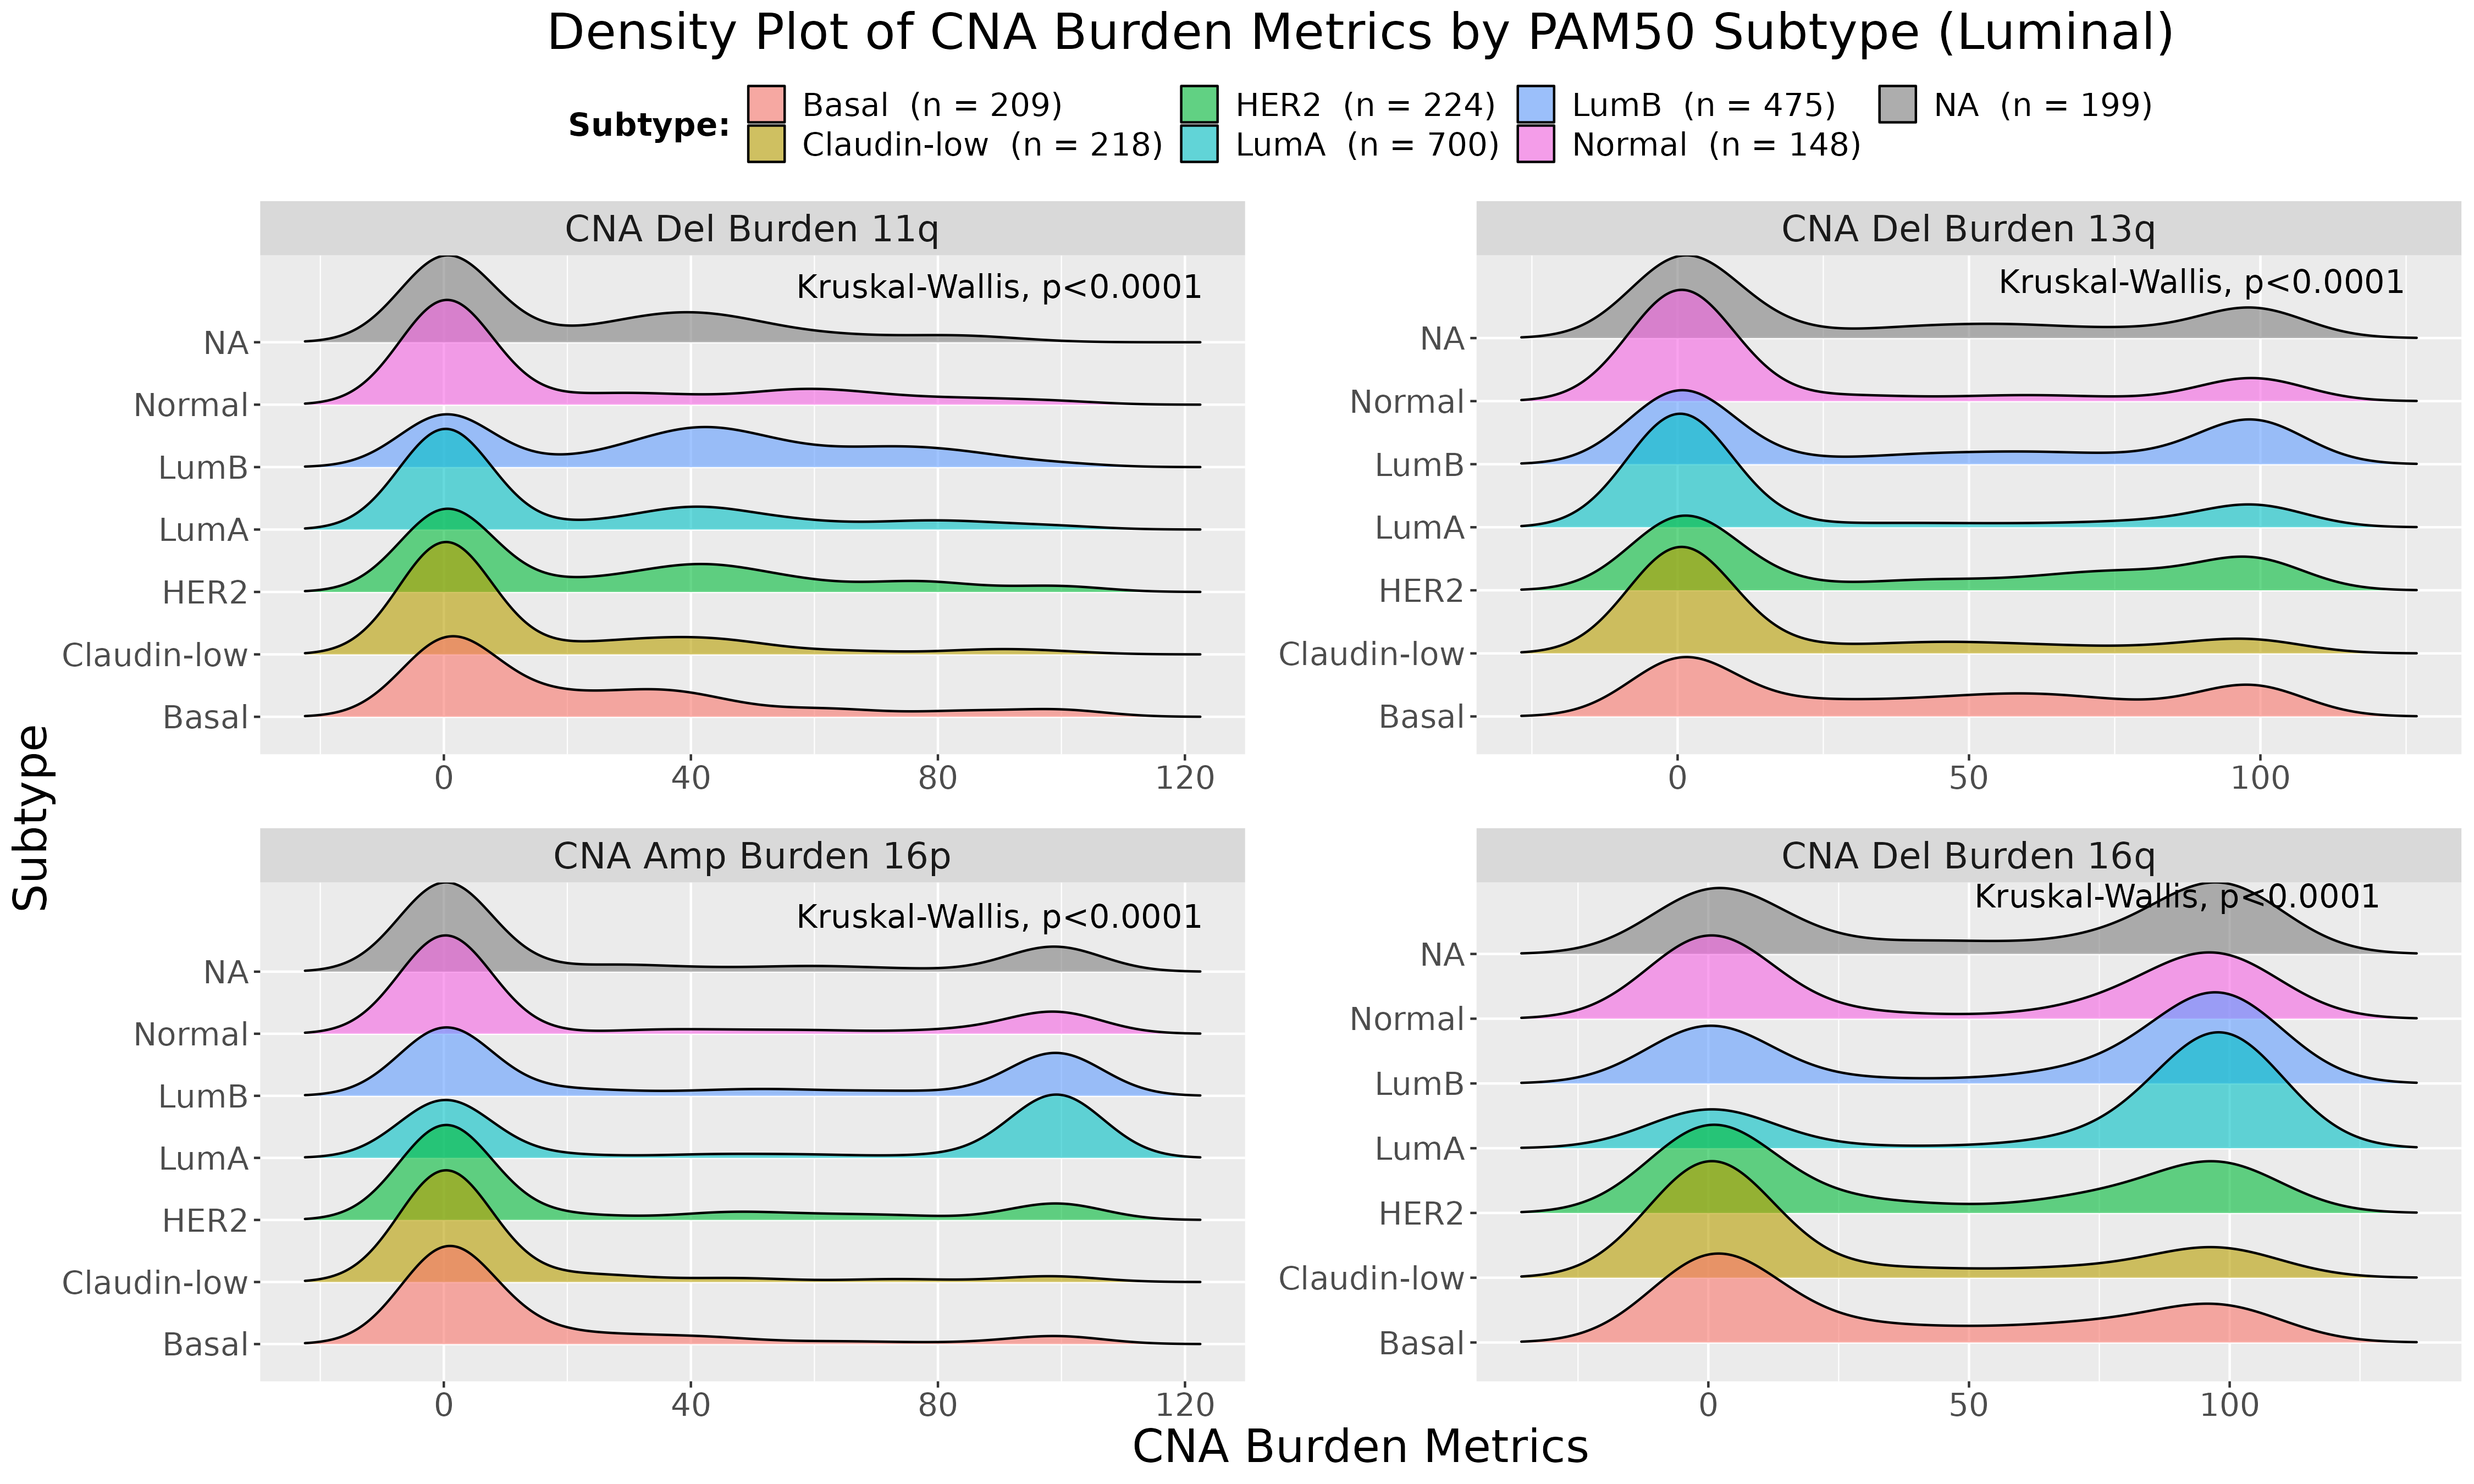
\includegraphics[width=1\textwidth]{../figures/Chapter_2/ChrArm_CNA_Burden_Metrics_Across_PAM50_Luminal_Burden.png}
\caption[Density plots for each selected chromosome arm CNA Burden metric, with a focus on the Luminal subtype.]{Density plots for each selected chromosome arm CNA Burden metric, with a focus on the Luminal subtype. Chromosome arms where Luminal patients display high GI are selected. Each facet contains boxplots for the chromosome arm CNA Burden metrics calculated using all available data and Benjamini-Hochberg adjusted Kruskal-Wallis p-values.}
\label{fig:PA-CNA-Score-Metric-Density-P50-16q}
\end{figure}

\begin{figure}[!htb]
\center
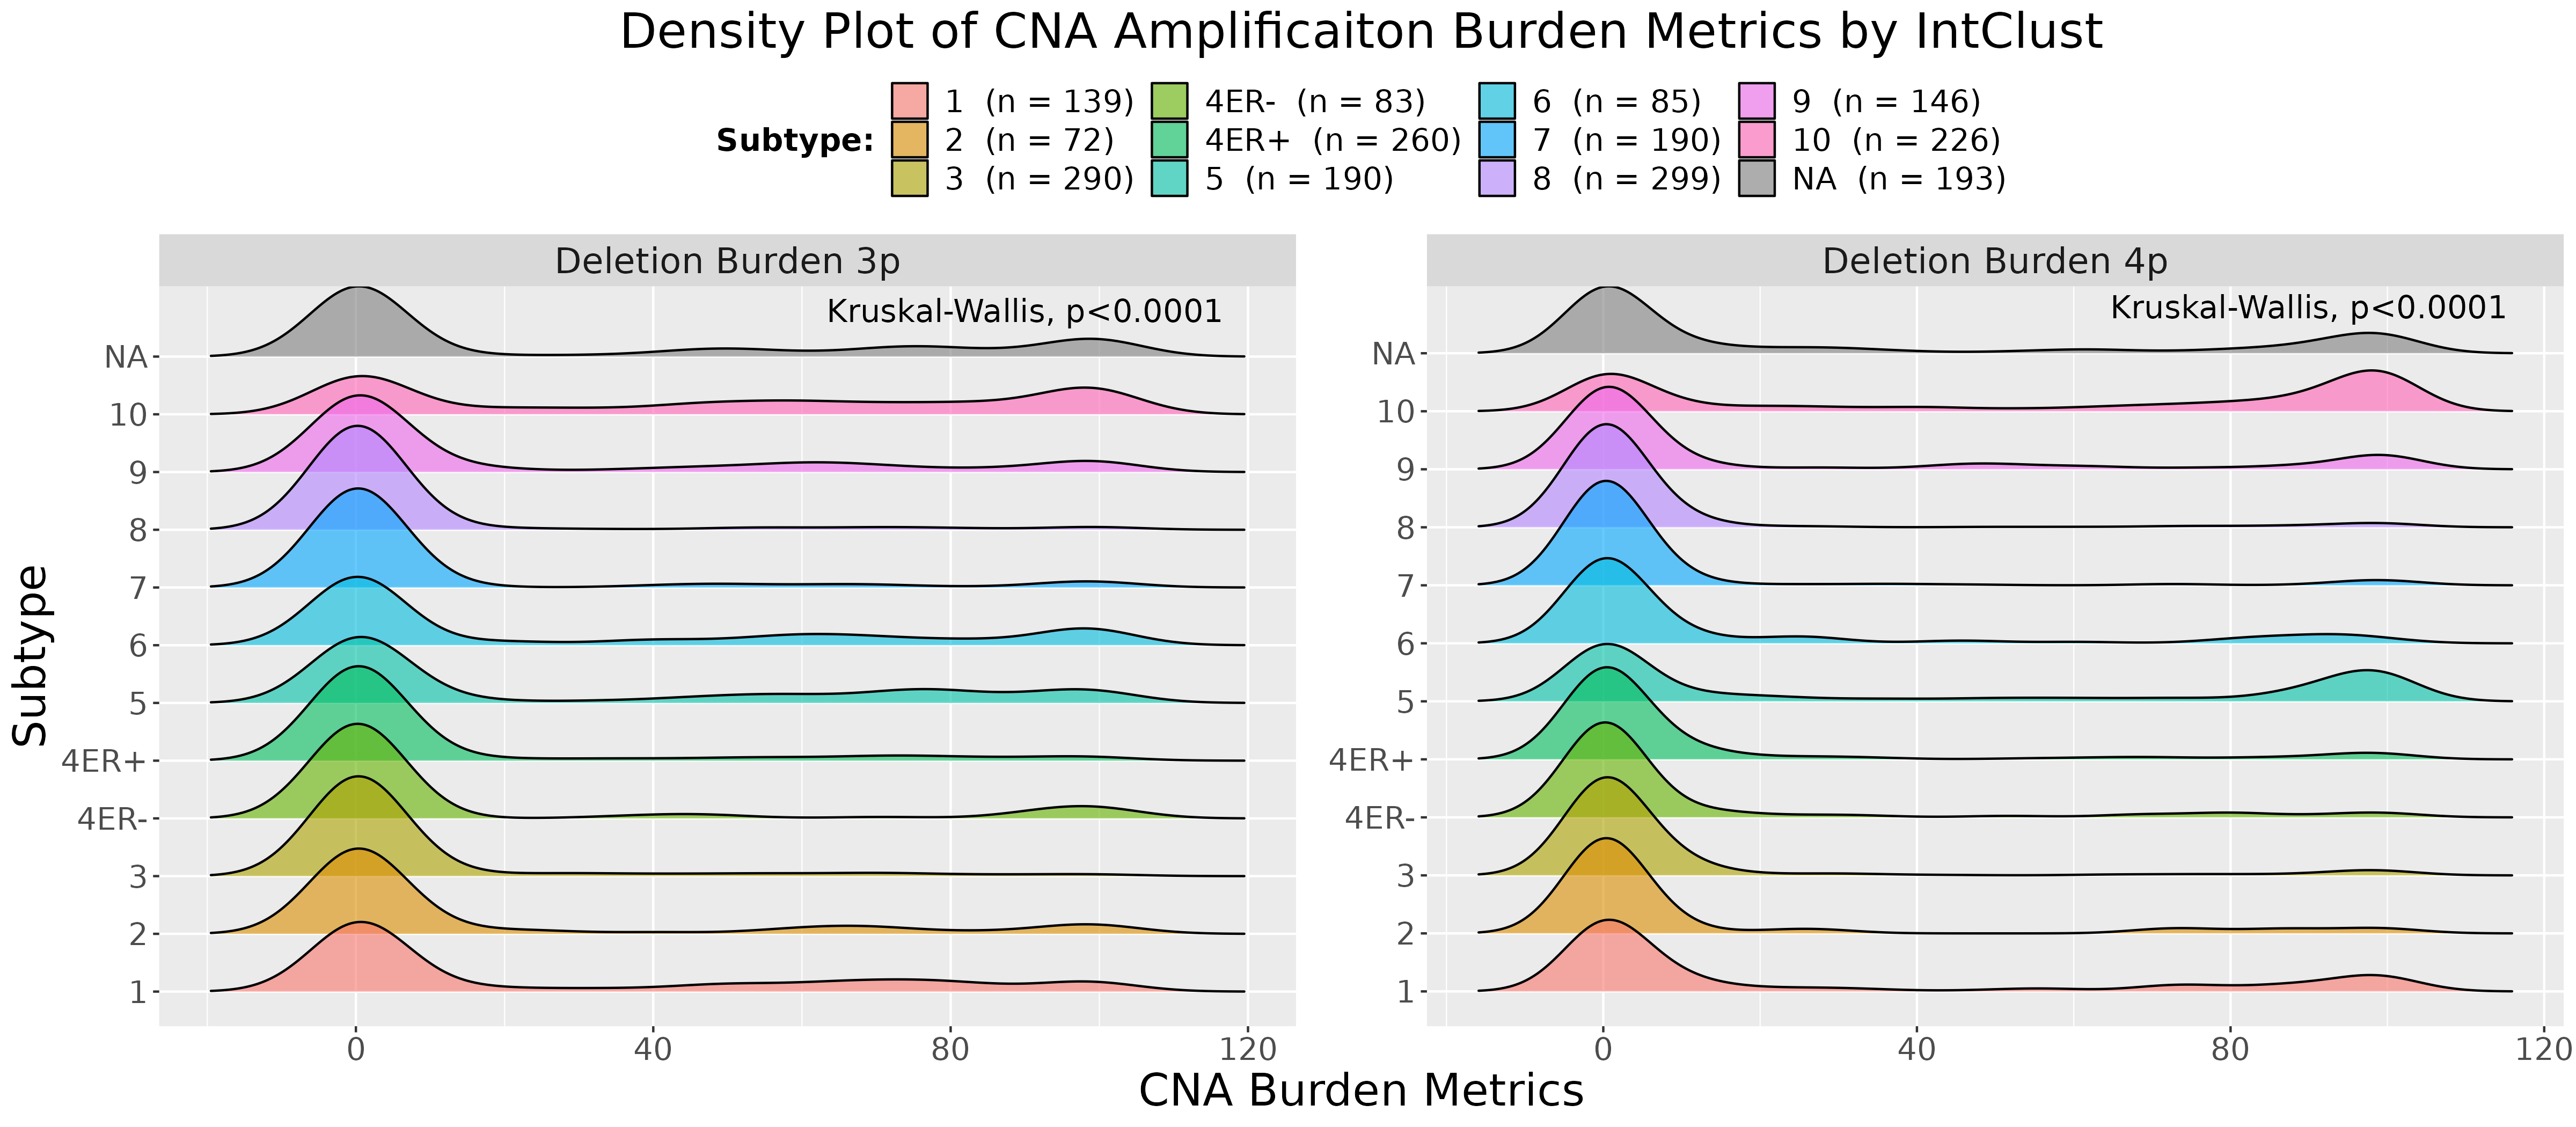
\includegraphics[width=1\textwidth]{../figures/Chapter_2/ChrArm_CNA_Burden_Metrics_Across_IC.png}
\caption[Density plots for each selected chromosome arm CNA Burden metric across Integrative Cluster.]{Density plots for each selected chromosome arm CNA Burden metric across Integrative Cluster. Each facet contains boxplots for the chromosome arm CNA Burden metrics calculated using all available data and Benjamini-Hochberg adjusted Kruskal-Wallis p-values.}
\label{fig:PA_IC}
\end{figure}

\begin{table}[!htb]
\center
\caption[Comparisons of selected chromosome arm CNA Burden metric distributions by PAM50 subtype, with a focus on the HER2 subtype.]{Comparisons of selected chromosome arm CNA Burden metric distributions by PAM50 subtype, with a focus on the HER2 subtype. Chromosome arms where HER2 patients display high GI are selected. Z statistics and Benjamini-Hochberg adjusted p-values are shown.}
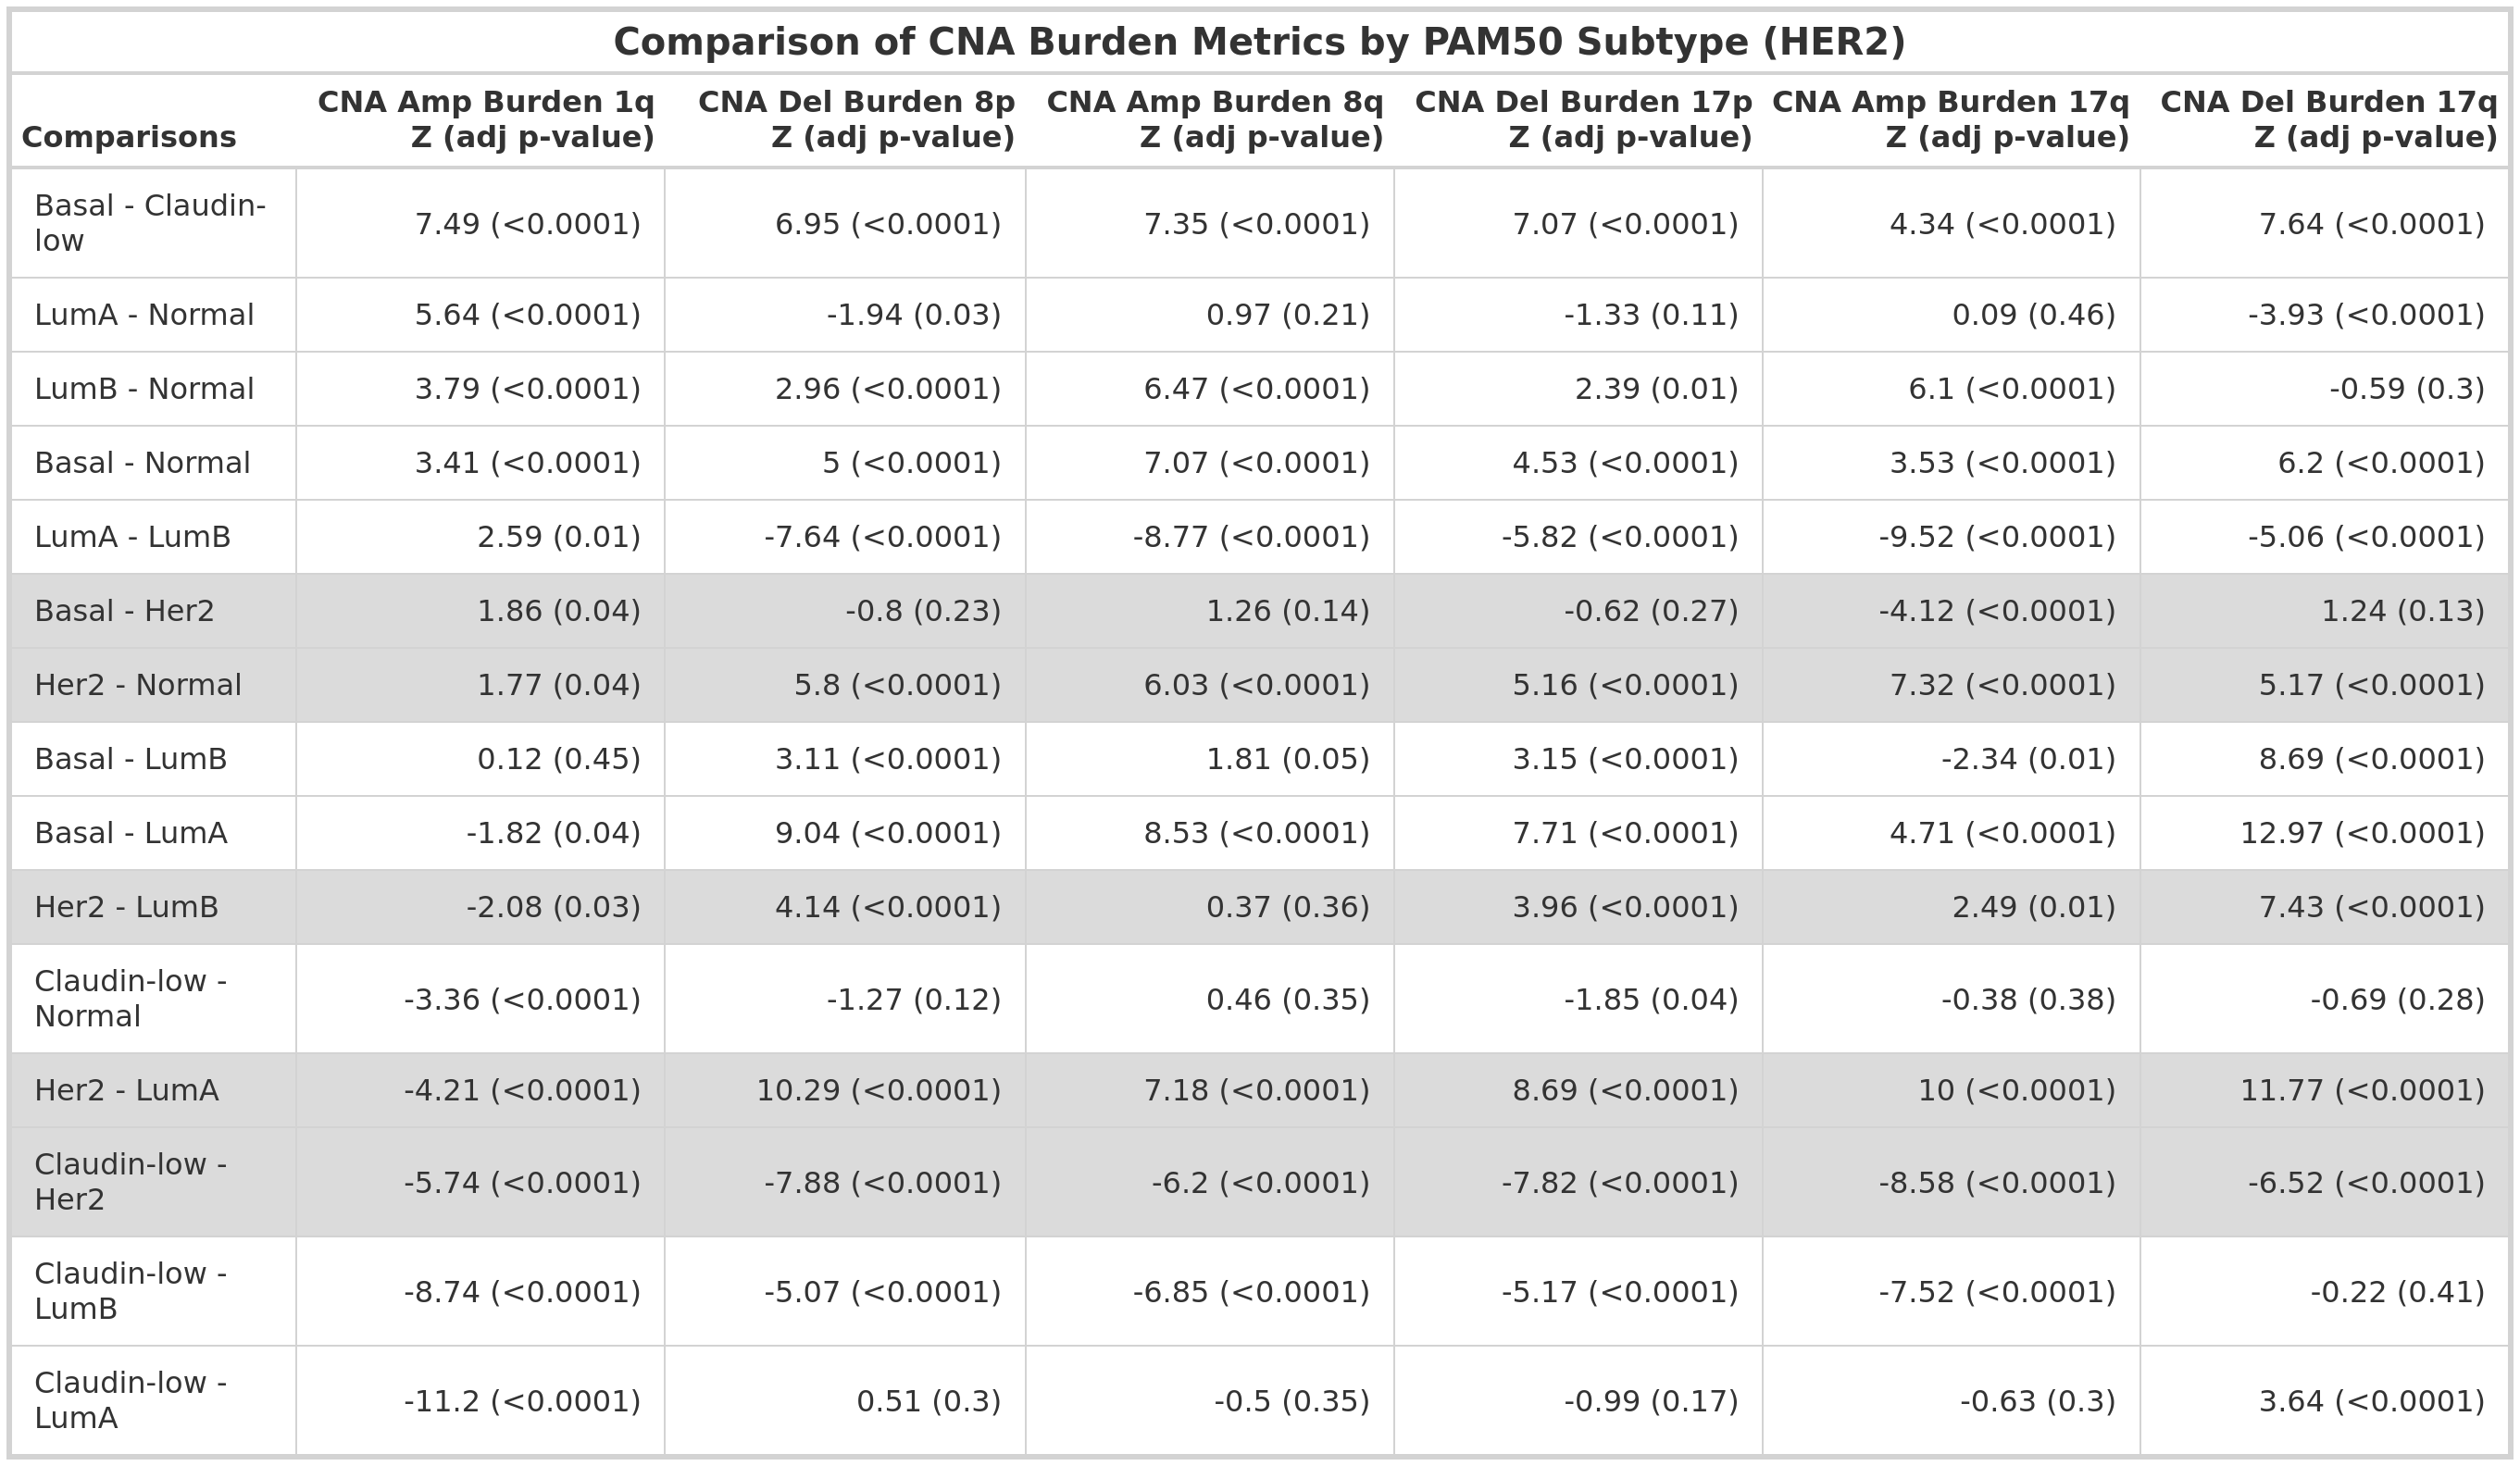
\includegraphics[width=0.9\textwidth]{../tables/Chapter_2/ChrArm_CNA_Burden_Metric_Comparisons_HER2.png}
\label{tab:PA-CNA-Score-Metric-Density-P50-17q}
\end{table}

\begin{table}[!htb]
\center
\caption[Comparisons of selected chromosome arm CNA Burden metric distributions by PAM50 subtype, with a focus on the Luminal subtype.]{Comparisons of selected chromosome arm CNA Burden metric distributions by PAM50 subtype, with a focus on the Luminal subtype. Chromosome arms where Luminal patients display high GI are selected. Z statistics and Benjamini-Hochberg adjusted p-values are shown.}
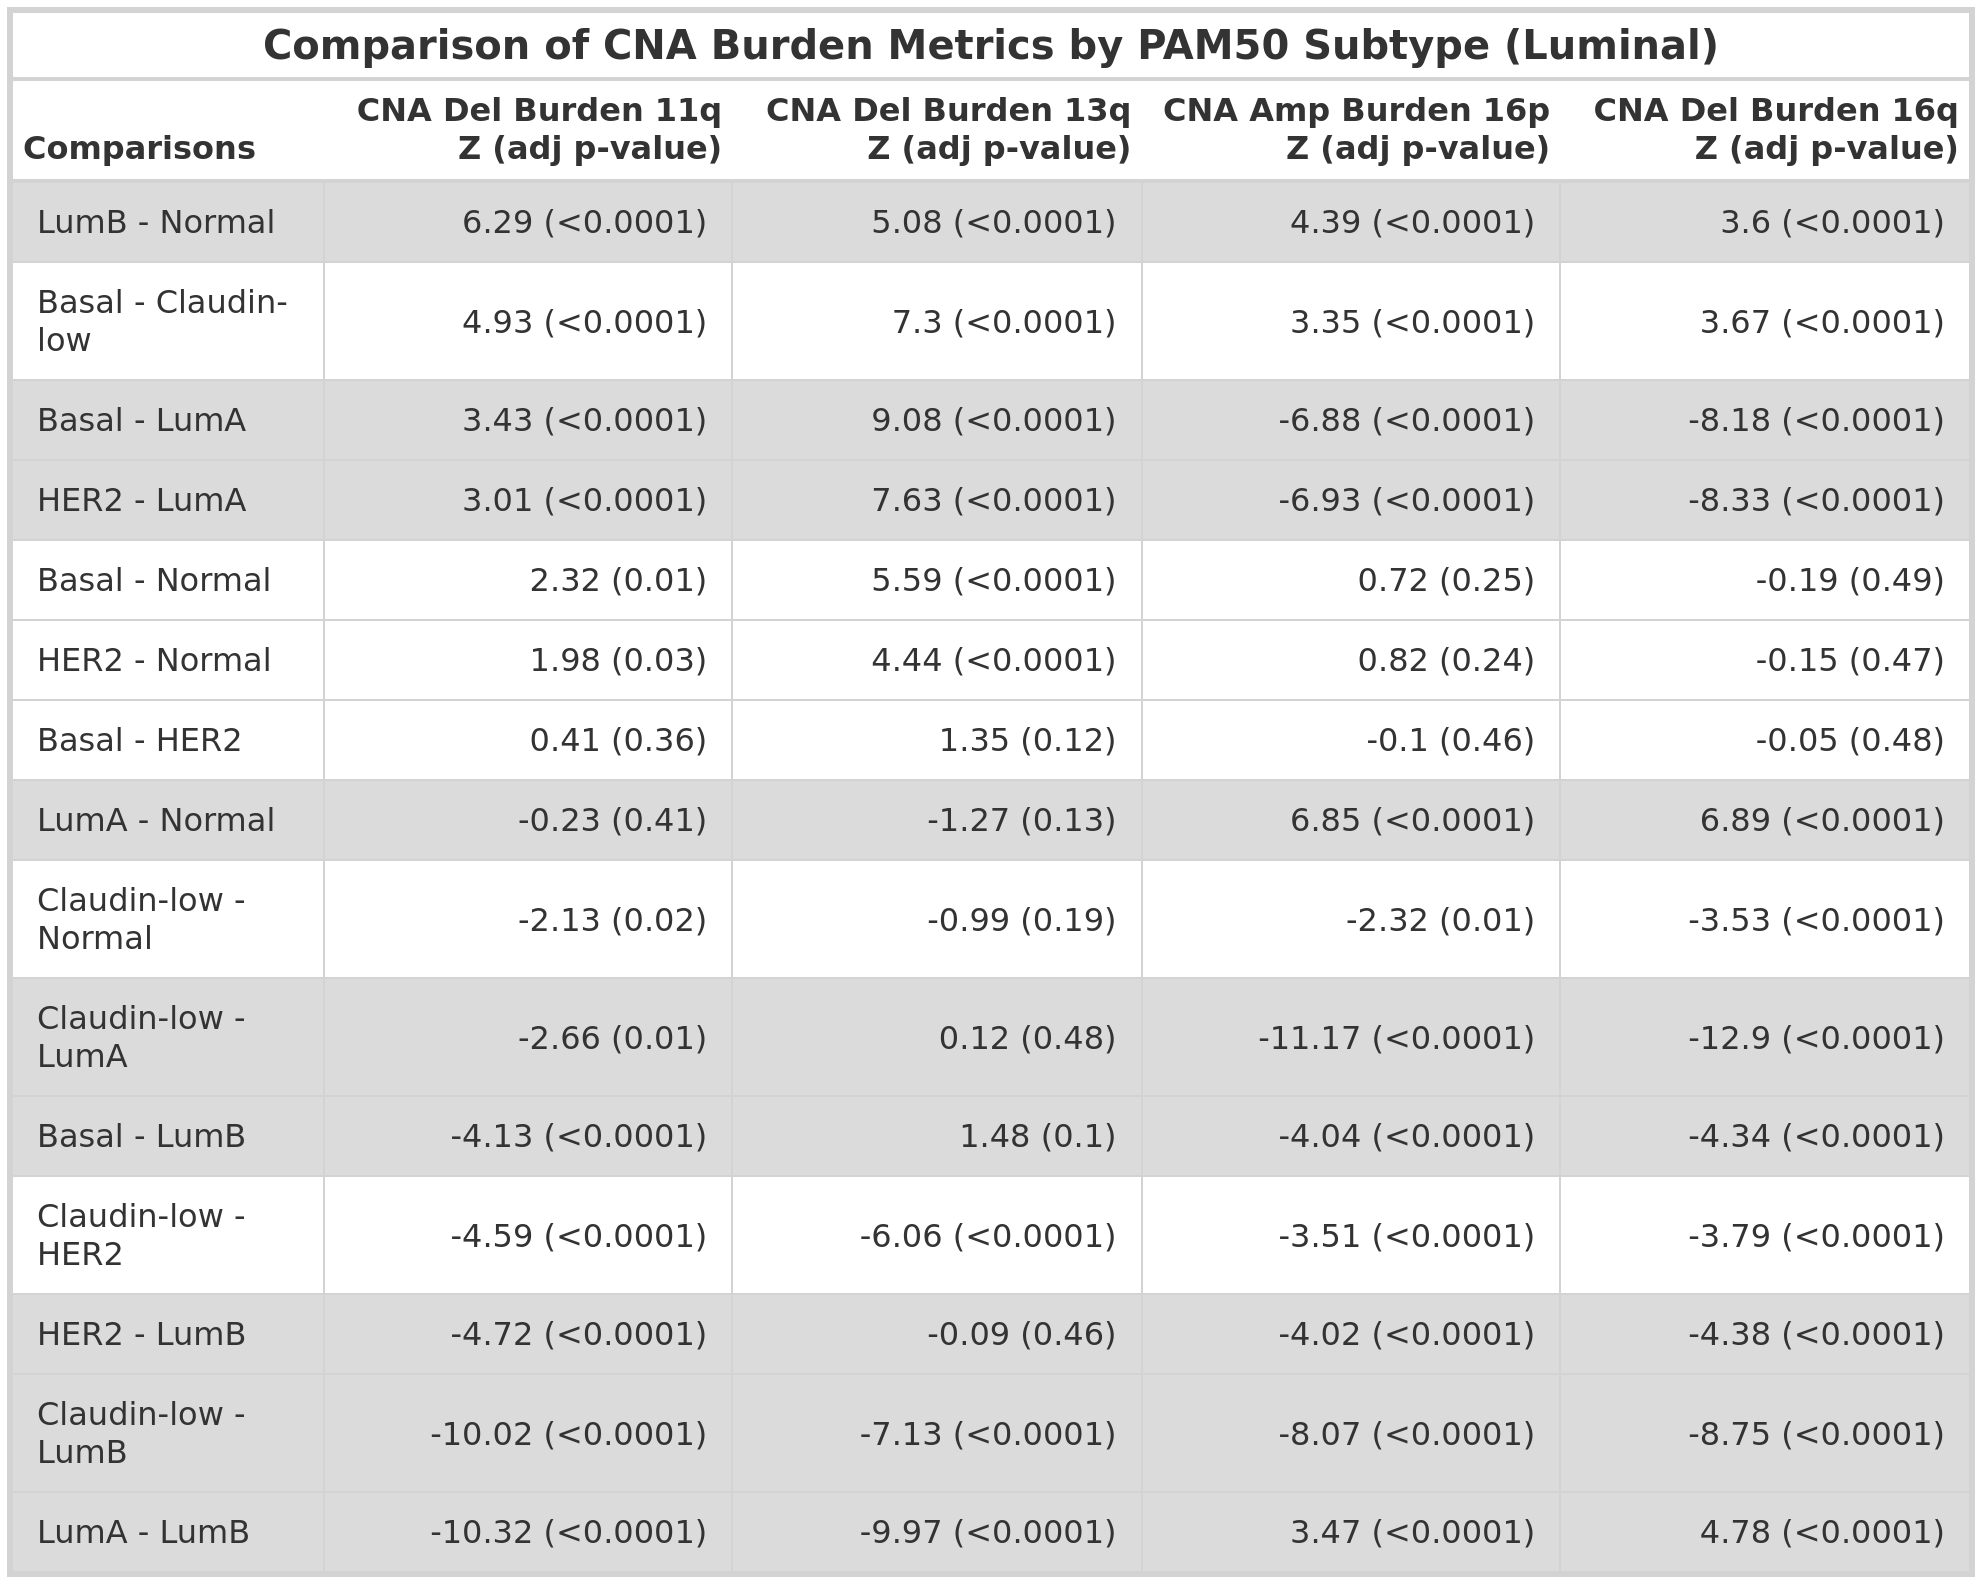
\includegraphics[width=0.9\textwidth]{../tables/Chapter_2/ChrArm_CNA_Burden_Metric_Comparisons_Luminal.png}
\label{tab:PA-CNA-Score-Metric-Density-P50-16q}
\end{table}

\begin{table}[!htb]
\caption[Comparisons of selected chromosome arm CNA Burden metric distributions by Integrative Cluster.]{Comparisons of selected chromosome arm CNA Burden metric distributions by Integrative Cluster. Z statistics and Benjamini-Hochberg adjusted p-values are shown.}
\begin{minipage}[c]{0.45\textwidth}
\centering
\begin{tabular}{ccc}
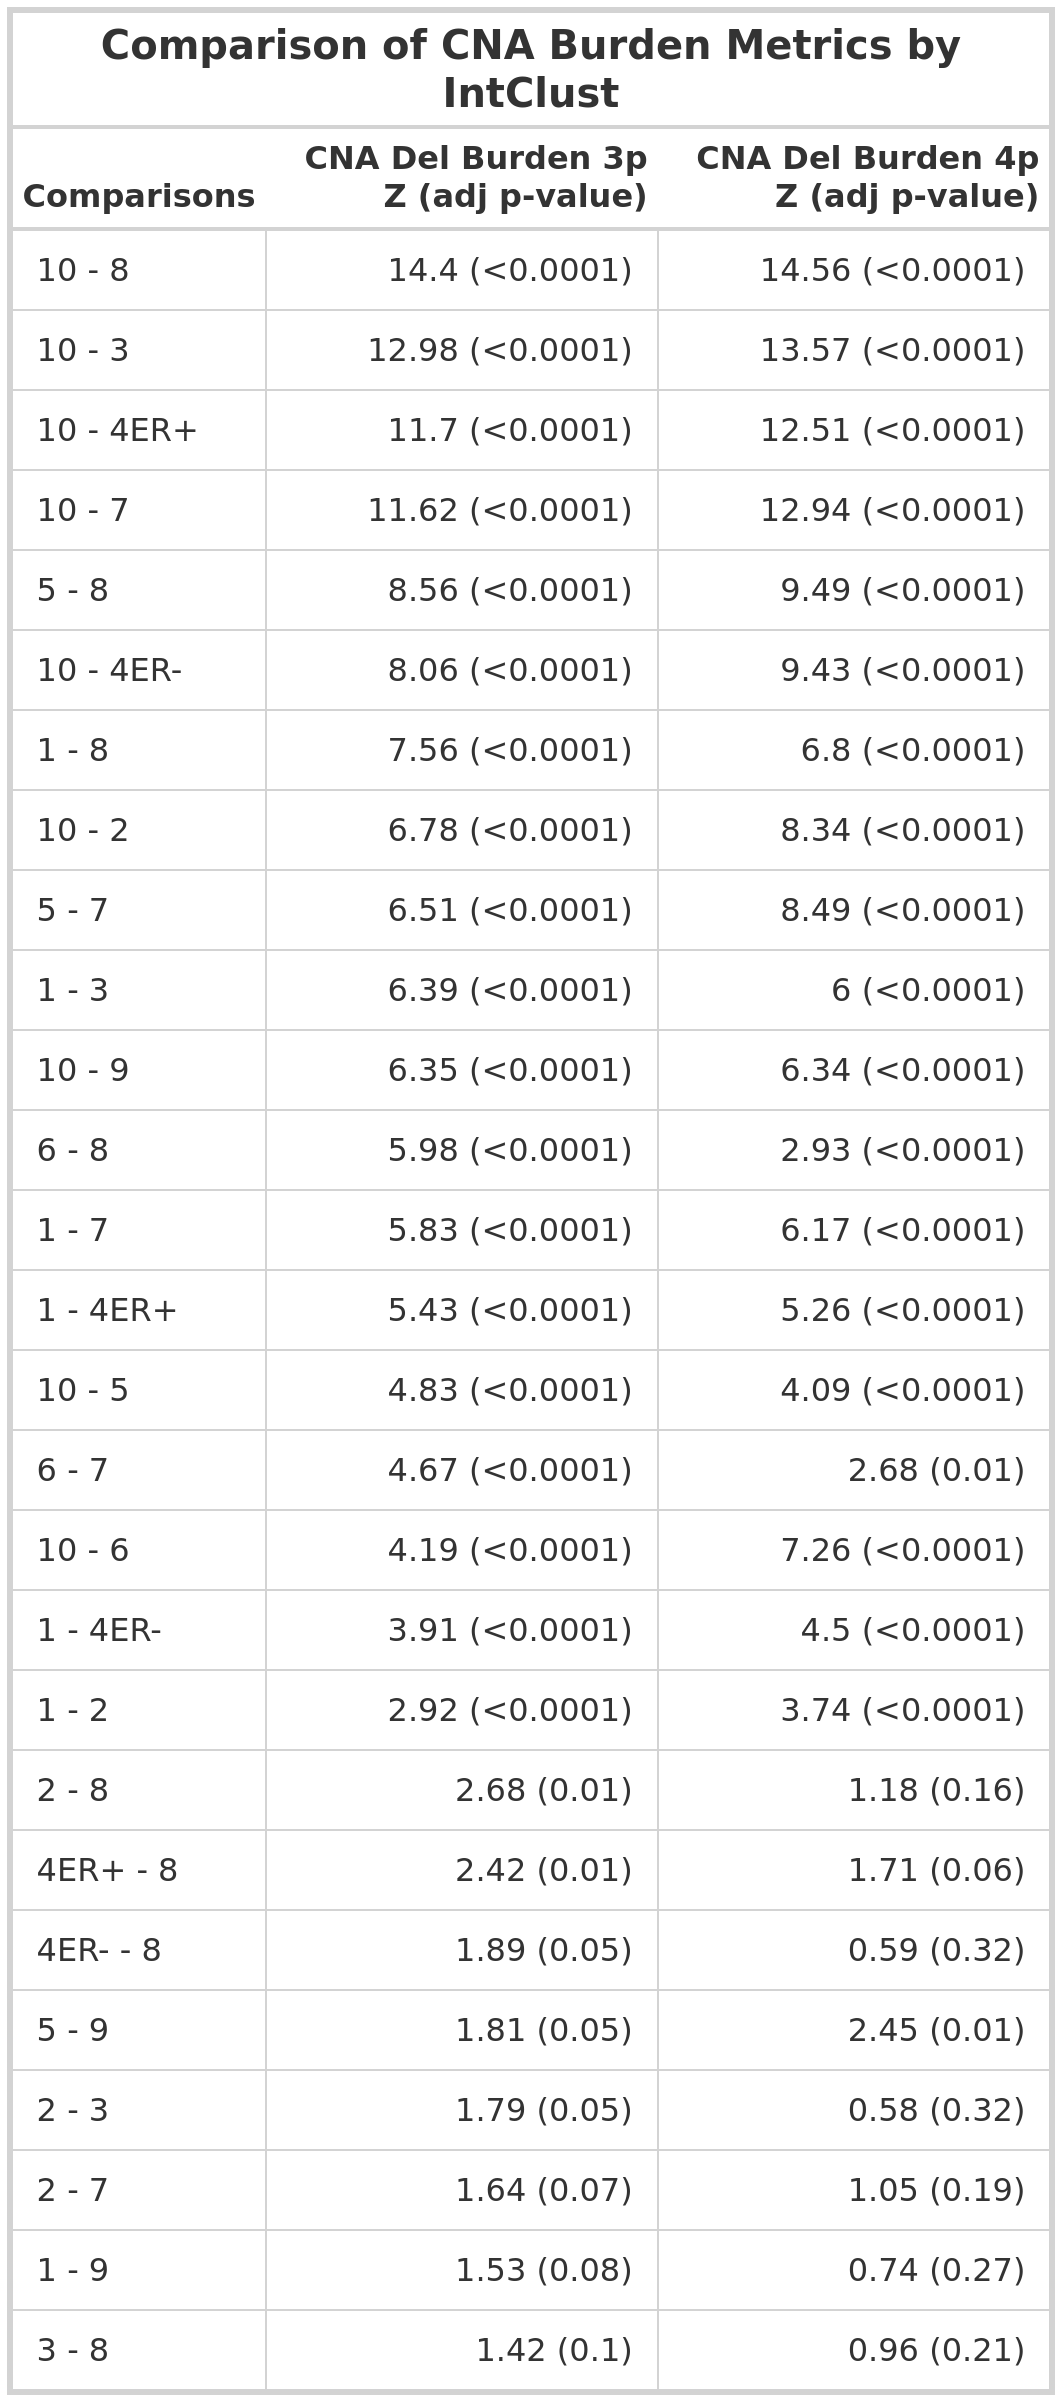
\includegraphics[width=0.98\textwidth]{../tables/Chapter_2/ChrArm_CNA_Burden_Metric_Comparisons_IC_1.png}
\end{tabular}
\end{minipage}
\hspace{0.8cm}
\begin{minipage}[c]{0.45\textwidth}
\centering
\begin{tabular}{ccc}
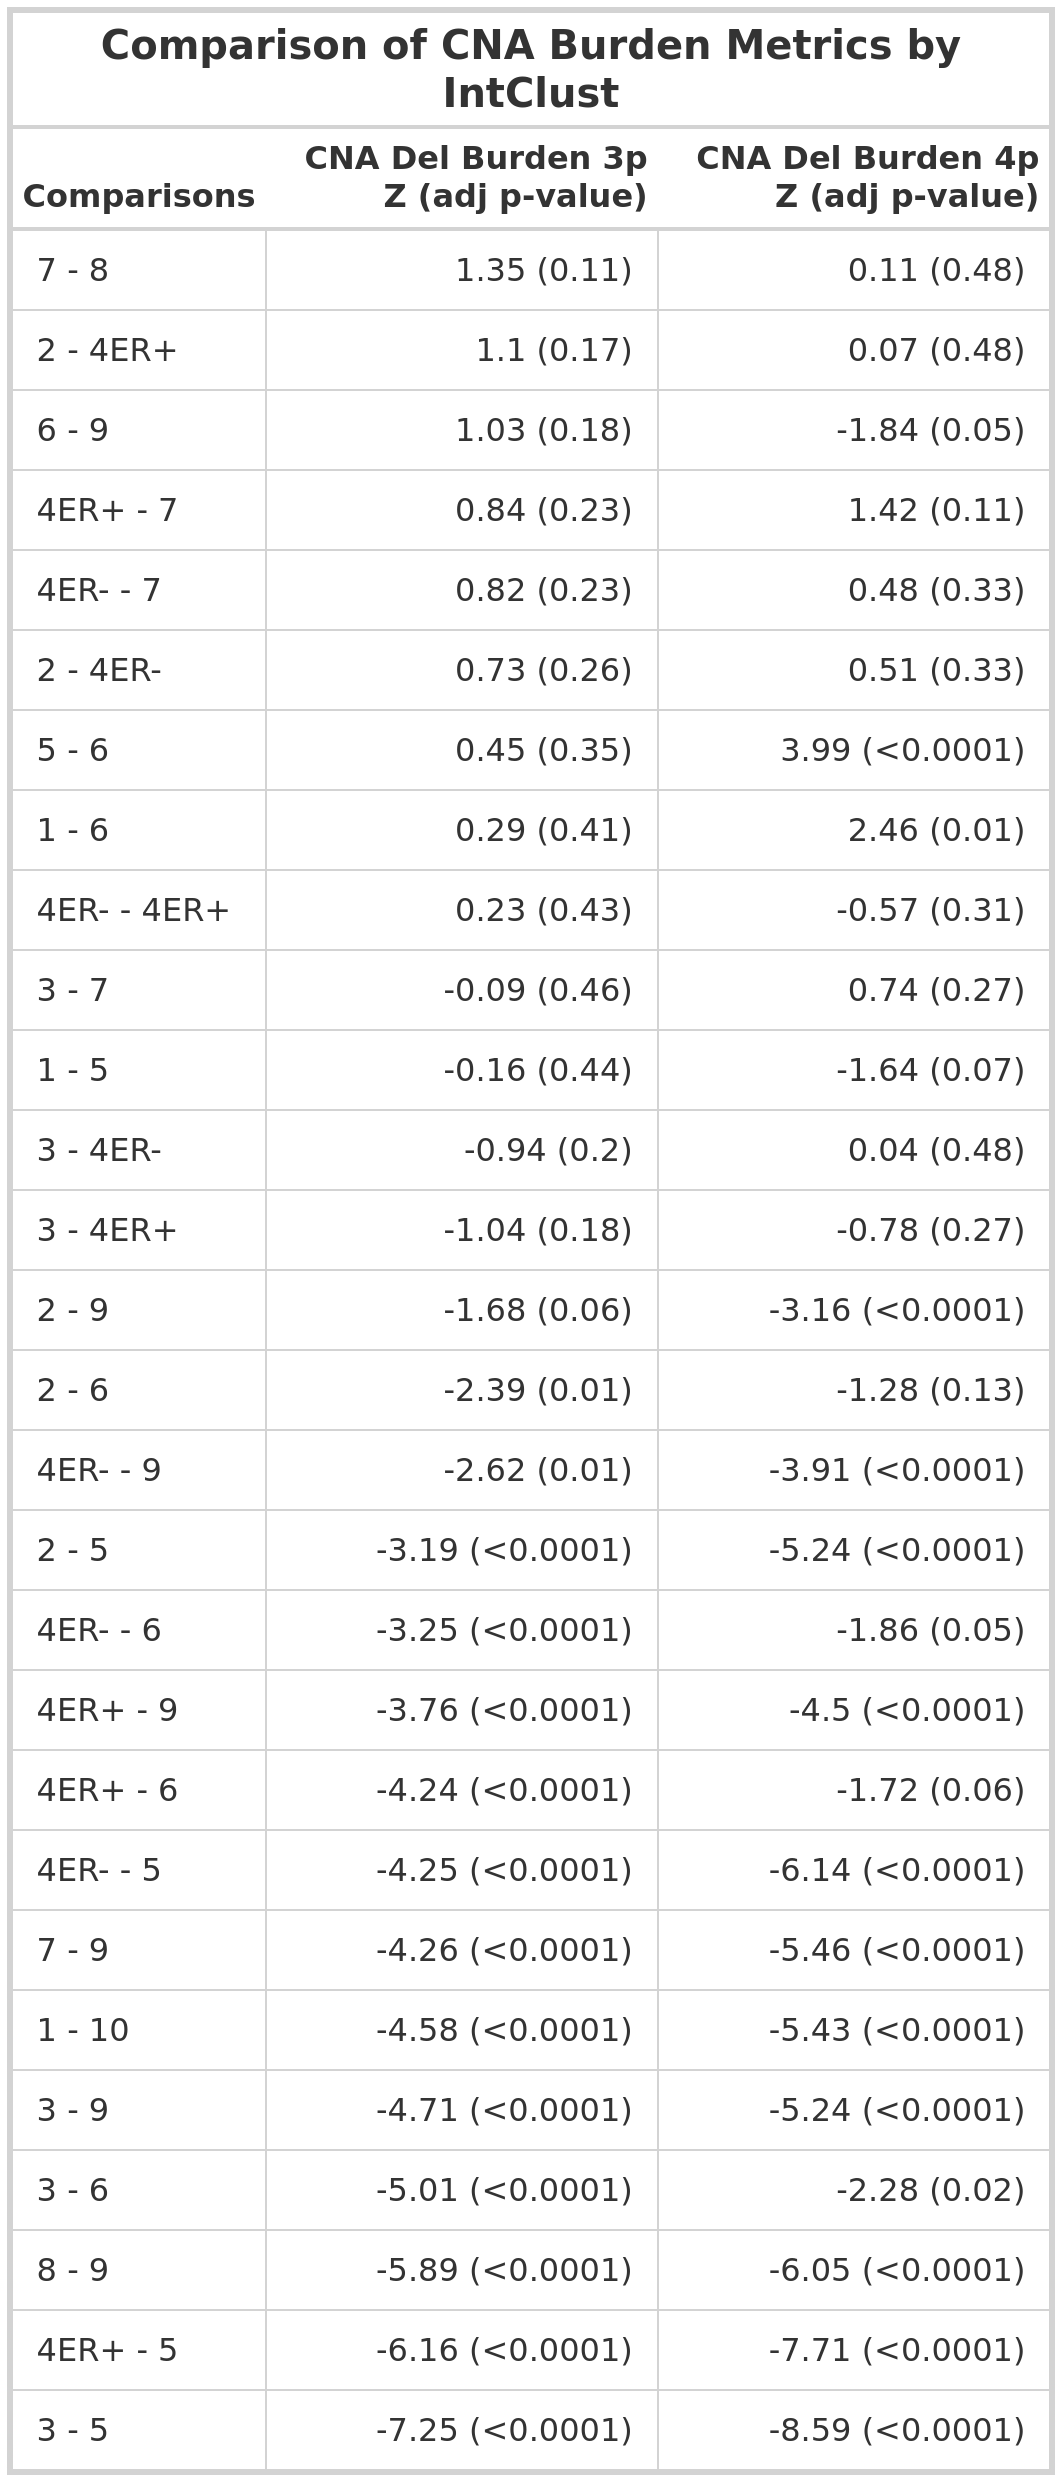
\includegraphics[width=0.96\textwidth]{../tables/Chapter_2/ChrArm_CNA_Burden_Metric_Comparisons_IC_2.png}
\end{tabular}
\end{minipage}
\label{tab:PA_IC}
\end{table}
\clearpage 

\subsection{Conclusions}
GI plays an important role in the initiation and progression of cancer and can influence patient prognosis. There are myriad ways to try to quantify the levels of GI within tumour samples, from both gene expression and CNA data, a number of these and their limitations have been discussed in this chapter.

We proposed a number of novel CNA Score and Burden metrics quantifying GI of a patient, calculated globally across the full genome and for each chromosome arm. These comprehensible metrics, applicable to publicly available data, quantify GI in totality for all aberration types, and also quantify GI attributed to amplifications and deletions.

It was observed that the presence of missing values, in existence for some patients, has a negligible effect on both the global and chromosome arm CNA metric distributions. As a result, the approach of using all of the available patient CNA Score and Burden data, as opposed to including only complete cases, is adopted in the downstream analysis. Analysing distributions of the CNA metrics comparing groups of patients stratified by molecular classifications PAM50 and IntClust offered interesting observations. We see concordance with characteristic genomic aberrations documented previously, such as high quantification of deletion burden on chromosome 5q within Basal tumours and high quantification of amplification on chromosome 17q within HER2 tumours. Focusing on the direct comparison of levels of amplification metrics to deletion metrics, we observe the subtypes associated with worse OS and DSS tend to have significantly higher quantified deletion burden. As the deletion landscape of breast cancer has been poorly characterised, our novel findings that PAM50 and IntClust classifications with poorer OS and DSS have higher levels of GI, in particular higher CNA deletion burden, encourage further investigation.

In the next chapter we investigate how the quantified levels of CNA Scores and Burden correlate with survival outcomes. 
